%%%%%%%%%%%%%%%%%%%%%%%%%%%%%%%%%%%%%%%%%%%%%%%%%%%%%%%%%%%%%%%%%%%%%%%%%%%%%%%%
%% Plantilla de memoria en LaTeX para la ETSIT - Universidad Rey Juan Carlos
%%
%% Por Gregorio Robles <grex arroba gsyc.urjc.es>
%%     Grupo de Sistemas y Comunicaciones
%%     Escuela T?cnica Superior de Ingenieros de Telecomunicaci?n
%%     Universidad Rey Juan Carlos
%% (muchas ideas tomadas de Internet, colegas del GSyC, antiguos alumnos...
%%  etc. Muchas gracias a todos)
%%
%% La ?ltima versi?n de esta plantilla est? siempre disponible en:
%%     https://github.com/gregoriorobles/plantilla-memoria
%%
%% Para obtener PDF, ejecuta en la shell:
%%   make
%% (las im?genes deben ir en PNG o JPG)

%%%%%%%%%%%%%%%%%%%%%%%%%%%%%%%%%%%%%%%%%%%%%%%%%%%%%%%%%%%%%%%%%%%%%%%%%%%%%%%%

\documentclass[a4paper, 12pt]{book}
%\usepackage[T1]{fontenc}

\usepackage[a4paper, left=2.7cm, right=2.7cm, top=3cm, bottom=3cm]{geometry}
\usepackage{times}
\usepackage[latin1]{inputenc}
%\usepackage[spanish]{babel} % Comenta esta l?nea si tu memoria es en ingl?s
\usepackage{url}
%\usepackage[dvipdfm]{graphicx}
\usepackage{graphicx}
\usepackage{float}  %% H para posicionar figuras
\usepackage[nottoc, notlot, notlof, notindex]{tocbibind} %% Opciones de ?ndice
\usepackage{latexsym}  %% Logo LaTeX

\usepackage{color}
\usepackage{xspace}
\usepackage{adjustbox}
\usepackage{multirow}
\usepackage{amsmath}
\usepackage{centernot}
\usepackage{tikz}


\usepackage{booktabs}
\usepackage{multirow}
%\newcommand{\gema}[1]{{\color{blue}\emph{Gema says: #1}\xspace}} %Comentarios del autor

\title{ Towards an Empirical Model to Identify When Bugs are Introduced}
\author{Gema Rodr\'iguez P\'erez}

\renewcommand{\baselinestretch}{1.5}  %% Interlineado

\newif\ifdraft
\drafttrue
\newcommand{\FFC}{\emph{FFC}\xspace}
\newcommand{\BIC}{\emph{BIC}\xspace}
\newcommand{\NoBIC}{\emph{BIC}\xspace}
\newcommand{\BFC}{\emph{BFC}\xspace}
\newcommand{\BFS}{\emph{BFS}\xspace}
\newcommand{\TSB}{\emph{TSB}\xspace}
\newcommand{\BIS}{\emph{BIS}\xspace}
\newcommand{\ACS}{\emph{ACS}\xspace}
\newcommand{\DCS}{\emph{DCS}\xspace}
\newcommand{\ac}{\emph{ac}\xspace}
\newcommand{\LC}[1]{\ensuremath{LC(#1)}\xspace}

\newcommand{\pc}{\emph{pc}\xspace}
\newcommand{\ipc}[2]{\ensuremath{pc(#1,#2)}\xspace}
\newcommand{\pcCBL}{\emph{CBL}\xspace}

\newcommand{\trueBIC}{\emph{trueBIC}\xspace}
\newcommand{\falseBIC}{\emph{falseBIC}\xspace}
\newcommand{\PC}[1]{\ensuremath{PCS(#1)}\xspace}
\newcommand{\ACSet}[1]{\ensuremath{ACS(#1)}\xspace}
\newcommand{\DCSet}[1]{\ensuremath{DCS(#1)}\xspace}


\newcommand{\setBFC}[1]{\ensuremath{BFC(#1)}}
\newcommand{\setBIC}[1]{\ensuremath{BIC(#1)}}
\newcommand{\setNoBIC}[1]{\ensuremath{NOBIC(#1)}}
\newcommand{\setSZZFound}[1]{\ensuremath{PCSZZ(#1)}}
\newcommand{\setSZZtoken}[1]{\ensuremath{PCtoken(#1)}}
\newcommand{\setSZZline}[1]{\ensuremath{PCline(#1)}}
\newcommand{\setTrueBIC}[1]{\ensuremath{TrueBIC(#1)}}
\newcommand{\setFalseBIC}[1]{\ensuremath{FalseBIC(#1)}}
\newcommand{\setTRUEPositives}[1]{\ensuremath{TruePos(#1)}}
\newcommand{\setFALSEPositives}[1]{\ensuremath{FalsePos(#1)}}



\newcommand{\rqPrevChanges}{When a line is changed to fix a bug, how frequently was this line the cause of a bug?}
 \newcommand{\rqPrevBIC}{When a line is changed to fix a bug, how frequently is its previous change the cause of a bug?\xspace}

 


\ifdraft
  \newcommand{\dmg}[1]{{\color{blue}\emph{Daniel says: #1}}\xspace}
  \newcommand{\gemaTODO}[1]{{\color{red}\emph{Gema MUST do: #1}}\xspace}
  \newcommand{\gema}[1]{{\color{green}\emph{Gema says: #1}}\xspace}
  \newcommand{\grex}[1]{{\color{orange}\emph{Gregorio says: #1}}\xspace}
  \newcommand{\jgb}[1]{{\color{red}\emph{Jesus says: #1}}\xspace}
\else
  \newcommand{\dmg}[1]{}
  \newcommand{\grex}[1]{}
  \newcommand{\gema}[1]{}
  \newcommand{\gemaTODO}[1]{}
  \newcommand{\jgb}[1]{}
\fi



%%% Local Variables:
%%% mode: latex
%%% TeX-master: "bugIntroChanges.tex"
%%% End:


\begin{document}

%\renewcommand{\refname}{Bibliograf?a}  %% Renombrando
%\renewcommand{\appendixname}{Ap?ndice}

%%%%%%%%%%%%%%%%%%%%%%%%%%%%%%%%%%%%%%%%%%%%%%%%%%%%%%%%%%%%%%%%%%%%%%%%%%%%%%%%
% PORTADA

\begin{titlepage}
\begin{center}


\includegraphics[scale=0.5]{img/logoURJC.jpeg}

\vspace{1.5cm}

\LARGE
TESIS DOCTORAL
\vspace{0.4cm}

\LARGE
\emph{Towards an Empirical Model to Identify When Bugs are Introduced}
\vspace{0.8cm}

\textbf{\Large
Author :\\
\underline{Gema Rodr\'iguez P\'erez}}

\textbf{\Large
Director:\\
\underline{Dr. Jes\'us M. Gonz\'alez Barahona}}

\textbf{\Large
Subdirector :\\
\underline{Dr. Gregorio Robles}}

\vspace{1.5cm}

\large
\textbf{Programa de Doctorado en Tecnolog\'ias de la Comunicaci\'on}\\

\textbf{Escuela Internacional de Doctorado}

\vspace{1cm}

\large
2018
\end{center}
\end{titlepage}

\newpage
\mbox{}
\thispagestyle{empty} % para que no se numere esta pagina


%%%%%%%%%%%%%%%%%%%%%%%%%%%%%%%%%%%%%%%%%%%%%%%%%%%%%%%%%%%%%%%%%%%%%%%%%%%%%%%%
%%%% Para firmar
\clearpage
\pagenumbering{gobble}
\chapter*{}

\vspace{-4cm}
\begin{center}
\LARGE
\textbf{Doctoral Thesis}

\vspace{1cm}
\large
Towards an Empirical Model to Identify When Bugs are Introduced

\textbf{Author :} Gema Rodr\'iguez P\'erez \\
\textbf{Director :} Dr. Jes\'us M. Gonz\'alez Barahona\\
\textbf{Subdirector :} Dr. Gregorio Robles

\end{center}

\vspace{1cm}
The committee named to evaluate the Thesis above indicated, made up of the following doctors

\vspace{0.5cm}
\textbf{President:}

\vspace{0.5cm}
\textbf{Member:}

\vspace{0.5cm}
\textbf{Member:}

\vspace{0.5cm}
\textbf{Member:}

\vspace{0.5cm}
\textbf{Secretary:}


\vspace{1.2cm}
has decided to grant the qualification of:



\vspace{1cm}
\begin{flushright}
Fuenlabrada,  \qquad$\;\,$  \qquad\qquad\qquad\qquad  2018\\
\vspace{0.5cm}
The secretary of the committee.
\end{flushright}


%%%%%%%%%%%%%%%%%%%%%%%%%%%%%%%%%%%%%%%%%%%%%%%%%%%%%%%%%%%%%%%%%%%%%%%%%%%%%%%%
%%%% Dedicatoria

\chapter*{}
\pagenumbering{Roman} % para comenzar la numeracion de paginas en numeros romanos
\begin{flushright}
\textit{To my family and friends \\
for their patience and support }
\end{flushright}

%%%%%%%%%%%%%%%%%%%%%%%%%%%%%%%%%%%%%%%%%%%%%%%%%%%%%%%%%%%%%%%%%%%%%%%%%%%%%%%%
%%%% Agradecimientos

\chapter*{Acknowledgements}
%\addcontentsline{toc}{chapter}{Agradecimientos} % si queremos que aparezca en el ?ndice
\markboth{ACKNOWLEDGEMENTS}{ACKNOWLEDGEMENTS} % encabezado

This thesis is the result of three years of work where I have met incredible people from all around the world who have inspired me. Thus, I apologize in advance if I forget to mention someone important; if we have met and talked, you are also a part of this. I do not even know how to start or how I should start, but let's try\ldots  

First of all, I would like to start by thanking my supervisors Jes\'us and Gregorio. They are great professors and great people who have provided me with a lot of guidance and knowledge, and I am very privileged to have been their Ph.D. student. They taught me what it means to be a researcher and I had the invaluable opportunity to learn from their passion, ideas, and professionalism. Their continuous support during my thesis has been a valuable part in my Ph.D., and their advice as well as their assistance in conferences has helped me to establish my own network. They have provided me with the means to continue growing, and I would like to once again express my gratitude. After two Summer stays in Canada and one year visiting the Netherlands, you will finally get rid of me :). 

I would like to give special mention to Alicia and Dorealda who have always been there to help. I would also like to give special mention to all the Bitergians; they have made my daily work more orange and funny, and in times of mining more easy with their marvelous tools (advertising!). 

From a more personal side, I would also like to say some words in Spanish; it will be easier to understand for my family. Me gustar\'ia das las gracias sobre todo a mis padres, su paciencia, entendimiento y apoyo constante siempre han sido incondicionales. Durante los \'ultimos a\~nos hemos aprendido a vivir separados, con las ventajas y desventajas que eso conlleva. Pero sin embargo, a pesar de la distancia, ellos siempre han sabido c\'omo demostrarme y hacerme llegar su apoyo, tanto en los mejores momentos como en los peores. Desde que me fui del pueblo, siempre han sabido estar cerca en los d\'ias m\'as difi\'ciles. �Gracias pap\'as! De la misma manera, me gustar\'ia dar las gracias a mis abuelos, a pesar de que los t\'erminos \emph{Doctorado} y \emph{Software} les suenen un poco abstractos, siempre han sabido defender (y en ciertas ocasiones inventarse\ldots) lo que hago. Durante un tiempo, mi abuela explicaba que mi trabajo consist\'ia en encontrar a la gente ``mala'' que estropeaba el Internet, incluso en ocasiones llegu\'e a ser \emph{hacker} profesional seg\'un sus explicaciones, jajaja. Tambi\'en quiero agradecer a mi hermano, y mis amigos, en especial a Maca y Sol, por todo su apoyo, entender la vida de una estudiante de doctorado no es nada f\'acil, �imag\'inate que incluso trabajamos los fines de semana! Por \'utimo, quiero dedicar una l\'inea a mi mejor entrenador, siempre ha sabido como motivarme, y si no es por su empuje inicial, quiz\'a no estar\'ia escribiendo esto ahora, as\'i que �gracias Casta! 

I also would like to thank Alexander Serebrenik and Andy Zaidman. They hosted me during my last year, giving me the opportunity to be part of their research group. My experience in TuDelft and TuE has been personally and professionally enriching. Along with Daniel M. German and Ali Mesbah, they have helped me in improving my language, my research and communication skills along with my knowledge and lessons I've learned from other cultures. I do not have any doubt that these periods have been the best part in my Ph.D. I would like to thank them for their patience in trying to understand what (sometimes) I wanted to express, and for their tips. During these periods out of my research lab, I had the opportunity to meet so many Ph.D. students and post-docs students. I would like to mention Wesley Torres, Mauricio Verano, Danna Zhang, Andrea Soto, Saba and Quinn Hanam who were my lab mates and with whom I had a lot of fun. 

This last paragraph is to summarize my experience. I do not have any clue what is going to happen after finishing my Ph.D, probably a would try to find a post-doc but who knows\ldots  However, one of the lessons that I learned is that academic life is very difficult, you have to be able to handle stress, deadlines, proposals, students, family, friends, and of course, never give up. It is also however both challenging and exciting where you start building an academic family to share ideas, research works, projects, travels and fun. In the academia, you are continuously learning and teaching others your work and this is the part I very much enjoy. I don't know if my future would be as a professor but, in this case, I will always remember the lessons and talks that Gregorio gave me, I've had the best role models to follow. 

%%%%%%%%%%%%%%%%%%%%%%%%%%%%%%%%%%%%%%%%%%%%%%%%%%%%%%%%%%%%%%%%%%%%%%%%%%%%%%%%
%%%% Resumen

\chapter*{Abstract}
%\addcontentsline{toc}{chapter}{Resumen} % si queremos que aparezca en el ?ndice
\markboth{ABSTRACT}{ABSTRACT} % encabezado

Finding when bugs are introduced into the source code is important, because it is the first step to understand how code becomes buggy. However, finding when bugs are introduced is a difficult and tedious process that requires a significant amount of time and effort, to the point that it is not even clear how to define \emph{``when''} a bug is introduced. 

Considering that fixed bugs do not always present similar properties, it might make sense to think that they are introduced and manifested in different forms. It is essential to distinguish between these moments; the instance when a bug is introduced in a system must be understood as the moment when buggy lines are introduced into the source code, and it must be distinguished from the moment when a system manifests the failure. In the sense that, whether we would test the code in the moment of its writing to search for the bug, the test will fail when the bug is inserted in this moment and the test will pass when the bug is not inserted. In the second case, other reasons different from an insertion of buggy code caused that the bug manifests itself in lines of the code that were clean in the moment of writing. For instance, when the source code is using, calling external APIs that can change without any previous notification, causing that some lines manifest the failure and need to be modified to fix it.

%while the bug introduction moment refers to the action of inserting buggy lines into the source code, the bug manifestation refers to the fact of displaying a bug in some lines of the source code without the necessity of containing buggy lines. For example, the lines changed to fix the failure could be correct when inserting them into the source code of the project, however, external factors such as changes in external code caused that these lines had to be changed to fix the bug. Furthermore, it is fundamental to understand that a fault might manifest itself without a bug introduction moment exiting. For instance, when the source code is using, calling external APIs that can change without any previous notification, causing that some lines manifest the failure and a developer has to modify these lines to fix it. However, in this scenario, the fault was not introduced, because the modified lines that fixed it were not buggy at the time of inserting them. Thus, the relevant factor to understand the precision of an algorithm that attempts to identify the origin and cause of a bug relies on the importance of distinguishing between the bug manifestation and the bug introduction moment.

To distinguish between these moments, this dissertation proposes a model to determine how bugs appear in software products. This model has been proven useful for clearly defining the code change that introduced a bug, when it exists, and to find the reasons that lead to the appearance of bugs. The model is based on the concept of when bugs manifest for the first time, and how that can be determined by running a test; it also proposes a specialized terminology which helps to analyze formally the process.
The validity of the model has been explored with a careful, manual analysis of a number of bugs in two different open source systems. The analysis starts with changes that fixed a bug, from which a test to determine whether or not the bug is present is defined. The results of the analysis have demonstrated that bugs are not always inserted in the source code, and this phenomenon should be further investigated to improve other disciplines of software engineering. Furthermore, the model has also been put in the context of current literature about the introduction of bugs in source code. An interesting specific result of the model is that it provides a clear condition to determine if a given algorithm for identifying the change introducing a bug is correct or not when performing the identification. This allows (i) to compute the \emph{``real''} performance of algorithms based on tracking back the modified lines that fixed a bug, and (ii) a sound evaluation of those algorithms.

%This dissertation deals with the identification of ``when" and ``how" software bugs were introduced in source code. %Beside this is a challenging task, it is also an interesting exercise to understand and learn how accidentally bugs were inserted into the source code, because we may use this information to identify different bug patterns and prevent future bugs by warning developers. 
%Finding the origin of a bug is a tedious process that requires a significant amount of time and effort. In fact, there is a  problem in the current bug seeding literature due to the lack of definition of what inserting an error in the source code means.

%The current state-of-the-art techniques are based on tracking back the modified lines that fixed a bug to find the suspicious change that introduced it. However, these techniques cannot be validated, mainly due to two reasons: The lack of a comparison model that can be used by developers to compute the precision and recall of these current techniques, and, the lack of definition in determining what ``to introduce a bug" means. These reasons cause that these techniques are not able to distinguish between the bug insertion moment and the bug manifestation moment. 

%In the end, the problem refers to how we define the introduction of a bug in the source code as well as how we define the moment when this bug was introduced. Because until now, the methods used to identify the bug introduction moment cannot compute what is a ``real" false/true positive or true/false negative.

%This thesis makes four main contributions. First of all, we carry out a Systematic Literature Review \emph{(SLR)} on the credibility and reproducibility of a well-known SZZ algorithm used to identify code changes that introduced a bug. The results of the SLR show the impact that this algorithm has in the current literature%, and also helps us to understand whether researchers are aware of the limitations of such algorithm and whether they attempt to mitigate them to improve the credibility and reproducibility of the results by using other techniques or improving the current ones. 

%The second contribution gives a solution to the principal problem that this dissertation addresses. This solution describes a model able to explain when a bug was introduced into the source code and how researchers can identify this moment. % By definition, this model contemplates different scenarios which are not considered in the traditional literature such as the addition of only new lines to fix a bug. 
%The principal aim of this model is to build a framework that will be used to validate the results obtained from the use of other techniques and to compute the precision of different algorithms. Because this model allows researchers to produce the `` gold standard"\gema{explicar mejor que es}. Furthermore, this solution not only defines the model of identifying the bug introduction moment, but it also details where it can be applied. 

%The third contribution of the thesis is the application of the proposed model into two cases of study, Nova and ElasticSearch. Both projects were chosen because of the high activity and number of developers that are contributing to them. Furthermore, both projects use control version systems that keep the evolution and history of the projects. Finally, the fact that both projects are written in different programming languages makes more interesting to study how different errors were inserted and manifested in the source code of a project

%Finally, the last contribution of this thesis is the quantification of the SZZ algorithm and some variants of it. After obtaining the ``gold standard" we can compute how many false/true positives and false/true negatives perform this algorithm. That means, researchers can ``really" measure the precision and recall of algorithms used to find the moment of bug introduction. Furthermore, a significant contribution to the current state-of-the-art is the proposed terminology used in this dissertation, since it is the first time that anyone attempt to define each element and each set of elements belonging to the bug seeding process.

%and it proposes a specialized terminology used in this dissertation, since it is the first time that anyone attempt to define each element and each set of elements belonging to the bug seeding process.

\chapter*{Resumen}
%\footnote{En el ap\'endice B se puede encontrar un resumen suficiente en castellano que cumple con los requisitos del art\'iculo 22 de la ``Normativa reguladora de los estudios de doctorado de la Universidad Rey Juan Carlos" para las tesis que sean presentadas en otros idiomas diferentes del castellano.}}
%\addcontentsline{toc}{chapter}{Summary} % si queremos que aparezca en el ?ndice
\markboth{RESUMEN}{RESUMEN} % encabezado

Es importante encontrar cu\'ando se introducen los errores en el c\'odigo fuente, porque \'este es el primer paso para comprender c\'omo el c\'odigo se vuelve defectuoso. Sin embargo, encontrar realmente cu\'ando se introducen los errores es un proceso dif\'icil y tedioso que requiere una gran cantidad de tiempo y esfuerzo, hasta el punto de que ni siquiera est\'a claro c\'omo definir \emph{``cu\'ando''}  se introduce un error en el sistema.

Teniendo en cuenta que los errores que se han arreglado no siempre presentan propiedades similares, puede tener sentido pensar que se introducen y se manifiestan en diferentes momentos y formas, y es esencial distinguir entre estos momentos. El momento de inserci\'on de un error en un sistema debe entenderse como el momento en que se introducen l\'ineas defectuosas en el c\'odigo fuente y debe diferenciarse del momento en el que un sistema manifiesta el error por primera vez a pesar de que en ocasiones ambos momentos pueden ser el mismo. Para diferenciar estos momentos podemos pensar que, si pudi\'eramos testear el c\'odigo que falla en el momento en el que fue escrito y el test falla, implica que en ese momento se insertaron las l\'ineas err\'oneas.  Por el contrario, si el test pasa significa que en ese momento las l\'ineas no eran err\'oneas, por lo que no se insert\'o un error en el sistema y debido a  otras razones diferentes, el error se manifiest\'o. Por ejemplo, cuando se utiliza el c\'odigo fuente o se llama a APIs externas que pueden cambiar sin notificaci\'on previa, puede provocar que algunas l\'ineas manifiesten el error sin necesidad de ser introducido previamente.

Para distinguir entre estos momentos, esta tesis propone un modelo para determinar c\'omo aparecen los errores en los productos software. Este modelo ha demostrado ser \'util para definir claramente el cambio de c\'odigo que introdujo un error, cuando \'este existe, y para descubrir otras razones que conducen a la aparici\'on de errores. El modelo se basa en el concepto de cu\'ando se manifiestan los errores por primera vez, y c\'omo se pueden determinar a trav\'es de ejecutar una prueba; tambi\'en propone una terminolog\'ia especializada que ayuda a analizar formalmente el proceso. La validez del modelo ha sido explorada mediante el cuidadoso an\'alisis manual de una serie de errores en dos sistemas de c\'odigo abierto. El an\'alisis comienza con cambios que corrigieron un error, a partir del cual se define una prueba para determinar si el error est\'a presente o no. Los resultados del an\'alisis han demostrado que los errores no siempre se insertan en el c\'odigo fuente y que hay diferentes motivos para ello, por lo que este fen\'omeno deber\'ia investigarse m\'as a fondo para mejorar otras disciplinas de ingenier\'ia de software. Adem\'as, el modelo tambi\'en se ha puesto en el contexto de la literatura actual sobre la introducci\'on de errores en el c\'odigo fuente. Un resultado interesante y expec\'ifico extra\'ido del modelo es que proporciona una condici\'on clara para determinar si dado un algoritmo para identificar el cambio que introduce un error es correcto o no en la identificaci\'on. Esto permite calcular (i) el rendimiento \emph{``real''} de los algoritmos basados en el seguimiento de las l\'ineas que han sido modificadas para corrigir un error, y (ii) evaluar esos algoritmos.

%Localizar el momento en el que un error, que ha sido arreglado, fue introducido en el c\'odigo fuente de un proyecto es una buena pr\'actica para entender y aprender c\'omo se introducen los errores no intencionados en el c\'odigo fuente. De este modo, podemos incluso tratar de prevenirlos cuando encontramos ciertos patrones que se repiten en el tiempo en diferentes proyectos. Tambi\'en, entender c\'omo se introducen los errores nos sirve para alertar a los desarrolladores cuando est\'an modificando el c\'odigo fuente, en caso de que errores similares a los cambios que est\'an haciendo hayan sido localizados y arreglados en el pasado. Sin embargo, encontrar el origen de un error no es una tarea f\'acil, requiere tiempo y esfuerzo poder entender el motivo que causa el arreglo de un error. De hecho, en el estado del arte actual sobre como se encuentran errores que han sido arreglados existe un problema que impide la correcta localizaci\'on del origen del error, este problema se basa en la falta de definici\'on de lo que significa un ``error" en el c\'odigo fuente.
%
%Para encontrar el supuesto cambio que introdujo el error en el c\'odigo fuente, las t\'ecnicas actuales se basan en rastrear de las l\'ineas que han sido modificadas para arreglar el error. Sin embargo, estas t\'ecnicas no se pueden validar, principalmente debido a dos razones: la falta de un modelo de comparaci\'on que pueda ser utilizado por los desarrolladores para calcular la precisi\'on y el recall de las t\'ecnicas actuales. Y, la falta de definici\'on para determinar qu\'e significa el hecho de ``introducir un error ''. Estas razones hacen que las t\'ecnicas actuales no puedan distinguir entre el momento de inserci\'on del error y el momento de manifestaci\'on del error.
%
%Teniendo en cuenta que los errores que han sido arreglados no siempre presentan propiedades similares, tiene sentido pensar que dichos errores se insertaron y manifestaron en diferentes formas. Es esencial entender que estos momentos son diferentes; mientras que el momento de introducci\'on de un error se refiere a la acci\'on de insertar l\'ineas de c\'odigo fuente defectuosas, el momento de manifestaci\'on de un error se refiere al hecho de que algunas l\'ineas del c\'odigo fuente manifiesten el error, incluso sin la necesidad de contener l\'ineas defectuosas. Por ejemplo, cuando las l\'ineas que manifiestan el error estaban limpias en el momento en que se insertaron en el c\'odigo fuente del proyecto, sin embargo, factores externos como cambios en el c\'odigo de APIs externas provocaron que esas l\'ineas manifestaran el error. Adem\'as, es fundamental comprender que un error puede manifestarse sin la necesidad de que exista un momento de insercci\'on. Por ejemplo, cuando el c\'odigo fuente consume artefactos externos que pueden cambiar su c\'odigo fuente sin notificaci\'on previa, provocando que algunas l\'ineas manifiesten el error y consecuentemente un desarrollador tenga que modificar esas l\'ineas para solucionarlo. Sin embargo, en este escenario no se introdujo el error, porque las l\'ineas que fueron modificadas para arreglarlo no conten\'ian errores en el momento de ser insertardas. Por lo tanto, el factor relevante para comprender la precisi\'on de un algoritmo que intenta identificar el origen y la causa de un error se basa en ser capaz de distinguir entre la manifestaci\'on del error y el momento de introducci\'on del error.
%
%Al final, el problema se resume a entender c\'omo los investigadores definen el hecho de introducir un error en el c\'odigo fuente y c\'omo definen el momento en el que se introdujo ese error. Porque hasta ahora, los m\'etodos utilizados para identificar el momento de introducci\'on del error no pueden calcular lo que es un true/false positivo o true/false negativo.
%
%Esta tesis hace la cuatro contribuciones principales. La primera, para profundizar sobre el  problema actual a la hora de encontrar el origen del los errores, se ha llevado a cabo un estudio sistem\'atico de la literatura basado en la credibilidad y reproducibilidad del (actualmente) algoritmo m\'as usado para identificar la(s) supuesta(s) linea(s) que introdujeron el error. El resultado del estudio sistem\'atico de la literatura nos aporta una visi\'on general sobre el impacto que tiene este algoritmo en el estado del arte. Ademas, nos ayuda a entender si los investigadores son conscientes, o no, de las limitaciones que presenta este algoritmo y si intentan, o no, poner soluci\'on y mitigar las para aumentar la credibilidad de sus resultados.
%
%La segunda contribuci\'on, es la soluci\'on propuesta al problema de encontrar inequ\'ivocamente el origen del error. Nuestra propuesta, se centra en definir un modelo que explique como se introducen los errores en el c\'odigo fuente. El principal prop\'osito de este modelo es crear un marco de comparaci\'on para validar los resultados obtenidos en otras t\'ecnicas. Con este modelo, podemos comparar diferentes algoritmos y ver como de efectivos son. Un valor importante de este modelo es que, por definici\'on, contempla diferentes escenarios que son realmente dif\'iciles de considerar en la literatura tradicional, como por ejemplo; cuando solamente se han introducido nuevas l\'ineas para arreglar un error o, cuando el momento de introducci\'on del error no puede ser rastreado en la historia de las l\'ineas que han sido modificadas para arreglar el error. En esta tesis, no solo definimos la teor\'ia del modelo de introducci\'on de errores, si no que tambi\'en detallamos d\'onde se puede aplicar y a\~nadimos el valor crear manualmente un conjunto de datos que sirve como el ``est\'andar de oro "
%
%La tercera contribuci\'on de la tesis, es la aplicaci\'on del modelo propuesto sobre dos casos de estudio, Nova y ElasticSearch. La elecci\'on de ambos proyectos se basa en que ambos son proyectos con un alto grado de actividad y un gran n\'umero de desarrolladores. Adem\'as, usan sistemas de version de control para guardar la evoluci\'on del proyecto.
%
%Finalmente, la \'ultima contribuci\'on de esta tesis es la cuantificaci\'on del algoritmo SZZ. Despu\'es de obtener el "est\'andar de oro", podemos calcular el n\'umero de true/false positivos y true/false negativos que obtiene este algoritmo. Esto significa que los investigadores pueden ``realmente" medir la precisi\'on y el recall de los algoritmos utilizados para encontrar el origen del error. Adem\'as, otra contribuci\'on significativa al estado del arte actual es la terminolog\'ia propuesta que ha sido utilizada en esta disertaci\'on, ya que es la primera vez que un art\'iculo intenta definir cada elemento y cada conjunto de elementos pertenecientes al proceso de siembra de errores.


%%%%%%%%%%%%%%%%%%%%%%%%%%%%%%%%%%%%%%%%%%%%%%%%%%%%%%%%%%%%%%%%%%%%%%%%%%%%%%%%
%%%% Resumen en ingles

%%%%%%%%%%%%%%%%%%%%%%%%%%%%%%%%%%%%%%%%%%%%%%%%%%%%%%%%%%%%%%%%%%%%%%%%%%%%%%%%
%%%%%%%%%%%%%%%%%%%%%%%%%%%%%%%%%%%%%%%%%%%%%%%%%%%%%%%%%%%%%%%%%%%%%%%%%%%%%%%%
% INDICES %
%%%%%%%%%%%%%%%%%%%%%%%%%%%%%%%%%%%%%%%%%%%%%%%%%%%%%%%%%%%%%%%%%%%%%%%%%%%%%%%%

% Las buenas noticias es que los ?ndices se generan autom?ticamente.
% Lo ?nico que tienes que hacer es elegir cu?les quieren que se generen,
% y comentar/descomentar esa instrucci?n de LaTeX.

%%%% ?ndice de contenidos
\tableofcontents
%%%% ?ndice de figuras
\cleardoublepage
%\addcontentsline{toc}{chapter}{Lista de figuras} % para que aparezca en el indice de contenidos
\listoffigures % indice de figuras
%%%% ?ndice de tablas
\cleardoublepage
%\addcontentsline{toc}{chapter}{Lista de tablas} % para que aparezca en el indice de contenidos
\listoftables % indice de tablas


%%%%%%%%%%%%%%%%%%%%%%%%%%%%%%%%%%%%%%%%%%%%%%%%%%%%%%%%%%%%%%%%%%%%%%%%%%%%%%%%
%%%%%%%%%%%%%%%%%%%%%%%%%%%%%%%%%%%%%%%%%%%%%%%%%%%%%%%%%%%%%%%%%%%%%%%%%%%%%%%%
% MOTIVATION %
%%%%%%%%%%%%%%%%%%%%%%%%%%%%%%%%%%%%%%%%%%%%%%%%%%%%%%%%%%%%%%%%%%%%%%%%%%%%%%%%

\cleardoublepage
\chapter{Introduction}
\label{chap:Introduction} % etiqueta para poder referenciar luego en el texto con ~\ref{sec:intro}
\pagenumbering{arabic} % para empezar la numeraci?n de p?gina con n?meros


%Establishing a research territory:
%	a) By showing that the general research area is important, central, interesting, problematic, or relevant in some way. (opcional)
%	b) By introducing and reviewing items of previous research in the are (obligatory)

Software evolution is a very active field of research in software engineering \cite{mens2008introduction}. The term \emph{software evolution} lacks a standard definition, and it is often used as synonym of the term \emph{software maintenance}. The basic operations of software maintenance are software modifications which include maintenance fixing bugs, adapting when external components change or adding features. These modifications make it necessary to adapt the software, Brooks states that ``over 90\% of the costs of a typical system arise in the maintenance phase, and that any successful piece of software will inevitably be maintained" \cite{brooks1974mythical}. It is believed that these modifications lead to failures.

Software systems have always contained bugs\footnote{Likewise Li \emph{et al.} \cite{li2006have}, we use the words ``bug" and ``error" interchangeably }, and finding these bugs have occupied and will occupy much of the daily development and maintenance tasks of software developers. Following some of the Lehman's laws formulated in \cite{lehman1979understanding} and \cite{lehman1998evidence},  software systems evolve. \textbf{Lehman's first law - continuing change:} ``a system must be continually adapted or it becomes progressively less satisfactory", \textbf{Lehman's second law - increasing complexity:} ``as a system evolves, its complexity increases unless work is done to maintain or reduce it", and \textbf{Lehman's sixth law - continuing growth:} `` the functional content of an system must be continually increased to maintain user satisfaction over its lifetime". As consequence, some researchers claim that \textit{``
it is necessary to develop new theories and mathematical models to increase understanding of software evolution, and to invest in research that tries to bridge the gap between the what (i.e., understanding) of software evolution and the how (i.e., control and support) of software evolution''} \cite{mens2005challenges}. 

The industry average defect rate when it comes to creating software is around 1 to 25 bugs for every 1,000 lines of code~\cite{mcconnell2004code}. Furthermore, according to the report form the National Institute of Standards and Technology in 2002, software bugs cost around \$59.5 billion to the U.S. economy annually \cite{planning2002economic}. Software bugs have an impact direct and indirect in the costs of a company such as the customer loyalty, brand reputation, wasted time in development and maintenance phases, etc. Despite the use of a handful of techniques to detect and prevent errors, they are inevitable during the development of software products. However, they can be identified, fixed, or even prevented before they reach a production environment, which reveals the necessity to understand how bugs are introduced into the source code to minimize the chance of defects being introduced
%Starting with the big picture, software failures cost the worldwide economy $1.1 trillion in 2016. These failures were found at 363 companies, affected 4.4 billion customers, and caused more than 315 years of lost time. . IBM estimates that if a bug costs $100 to fix in Gathering Requirements phase, it would be $1,500 in QA testing phase, and $10,000 once in Production. When a company announces a software failure, they lose an average of $2.3 B of shareholder value just on the first day.

%As a consequence, developing and testing software systems is currently a huge challenge for software engineers.such as changes in the environment or user needs

%% the industry needs to understand how they are introduced to minimize the chance of them being introduced. 
%Despite the use of a handful of techniques to detect and prevent defects, they are inevitable during the development of software products. However, they can be identified, fixed, or even prevented before they reach a production environment. The industry average defect rate when it comes to creating software is around 1 to 25 bugs for every 1,000 lines of code~\cite{mcconnell2004code}. That reveals the necessity to understand how bugs are introduced into the source code to minimize the chance of defects being introduced. 

% Establishing a niche ( a particular microenvironment where a particular piece of research makes particularly good sense)
%	a) By indicating a gap in the previous research, raising a question about it, or extending previously knowledge in some way (obligatory)
This makes it specially important to understand the processes which leads to bugs manifesting and causing programs to malfunction. The bugs have been studied since the early 70's in software reliability~\cite{jelinski1972software}, developing models for predicting software reliability which are based on the observation of software product failures. However these models ignore information regarding the developments of the software, the environmental factors or the method of failure detection \cite{pham2000software}. A common practise in Empirical Software Engineering~\emph{(ESE)} to know how bugs are inserted, is based on the study of their reports, causes, and fixes. Specifically, the study of the changes that fix a bug is an interesting exercise which allows researchers to understand its importance in different areas of SE and come up with new techniques that practitioners can used. For example, determining why and how a bug is introduced may help to identify other potential changes that introduce bugs~\cite{sliwerski2005changes,kim2006automatic,zimmermann2006mining,thung2013automatic,sinha2010buginnings}; it may help to discover patterns of bug introduction that could lead to the discovery of methods to avoid them~\cite{nagappan2006mining,zimmermann2007predicting,hassan2009predicting,hassan2005top,kim2007predicting}; it may help to identify who is responsible for inserting the bug, which has the potential to propagate self-learning and peer-assessment processes~\cite{izquierdo2011developers,da2014unveiling,ell2013identifying}; it may help to understand how long a bug is present in a code, thereby enabling researchers and developers quantify the software quality and avoiding the misleading~\cite{rodriguez2017much,chen2014empirical,weiss2007long}, and so forth. Due to these reasons, this field of study has long been active during the last decades. 
 
There is a lot of information in software maintenance activities on how failures are reported, discussed and managed in issue tracking systems, such as Bugzilla, Launchpad or Jira. Although useful information to understand the bug may be missed or not documented in these systems \cite{aranda2009secret}, Panichella \emph{et al} observed that very often in open source projects, developers tend to use these issue tracking systems and mailing list to discuss and communicate with each others \cite{panichella2014developers},\cite{panichella2014evolution}. Thus, this sources of informations should be enough to provide a textual description regarding the \emph{symptoms} of the bug. Then, this information can be linked to the source code system that provides the \emph{treatment} through changing the source code to fix the error. 

In ESE finding when bugs are introduced is still difficult, to the point that it is not even clear how to define \emph{``when''} a bug is introduced.  As the term \emph{``bug''} is not clearly defined, sometimes it is mixed up with the term \emph{``feature''}, Herzig \emph{et al.} studied how to distinguish between bugs and features \cite{herzig2013s}. The study of what line of the source code inserted the bug is still a challenge, the researchers are merely adopting current assumptions that are already clarified in the literature, where it is established that the modified lines to fix the failure are likely the cause of the bug. %Due to the general use of this assumption, many researchers have start with this premise to carry out studies on the cause of a bugs, to improve the heuristics under this assumption. %There is a lack of experience in understanding the context and dependences of the \emph{moment of writing} the lines that have been modified or deleted to fix the bug. As such, there is a lack of research on how a bug is introduced into the system, and how that moment is defined. 

Currently, many researchers in ESE start with this assumption to conduct studies on identifying the bug introduction change through navigating back the modified lines of the change that fixed the bug. This approach, however, is ineffective in answering the relevant questions, \emph{``what caused the bug?''} and \emph{``was this line buggy in the moment of its insertion?''}, because it does not provide any mean of validation which developers can use to be sure whether or not the line identified in the approach contained the bug when it was written into the source code.

% My contributions
%Occupying the niche
%	a) by outlining purposes oir stating the nature of the present research (obligatory)
%	b) By announcing principal findings (optional)
% 	c) By indicating the structure of the research paper (optional)

%

Without this understanding, it is difficult to develop a successful approach to identify exactly when a bug is inserted into the software. To investigate and better understand how bugs appear in software products, this thesis introduces a model that defines the code change that introduced a bug. It is particularly important to clarify that a bug is only introduced in a system when buggy lines are introduced into the source code. This model also establishes the distinction between the bug introduction moment and the first moment when the bug manifested itself in the system.  Although both moments can be the same, they must be distinguished. These moments not only focus on studying the \emph{treatment}, they also analyze the \emph{symptoms}. By navigating back to the lines that have been changed to fix the failure, the history of the bug can be easier understood, and thereby it is theoretically possible to discover whether the lines modified to fix the bug introduced the bug or to confirm that other reasons lead to its appearance. The knowledge of this information can be very useful in many fields of Software Engineering. For example, when computing various metrics, such as the time it takes to notify a bug~\cite{rodriguez2017much} or the experience of the committer and their activity in the project~\cite{izquierdo2011developers,izquierdo2012more}. It allows improving advanced techniques that harness such information to learn patterns of these changes, to motivate the design and development of better mechanisms~\cite{harris2010transactional}, or to help to automate bug predictors that can estimate the likelihood of fault introduction by a given commit~\cite{rao2011retrieval,thung2012extent,zimmermann2007predicting}.

%; the moment of bug introduction can be identified by using a hypothetical test that checks whether the code in the moment of its writing presents the \emph{symptoms} described in the bug report:
%\begin{itemize}
%  \item When the test fails, it means that the lines were buggy at this time, and we can be sure that the bug was inserted in this moment. 
%  \item When the test passes, it means that the lines were clean at this time and that there was not a bug introduction moment. This is because a system has different needs at different points over time and the requirements of the system change and they might not be managed properly; for instance, a clean line inserted at moment \emph{A} may not cause the failure of the system, but when the project reaches moment \emph{B}, the line might trigger the bug causing the failure of the system. This is possible because the system is using external dependencies that will have changed between moment \emph{A} and \emph{B}. Another explanation could be that some external library has a bug which was inserted in moment \emph{B}. A third explanation also could be due to the evolution of the system which will trigger changes in other parts of the code thereby only affecting the code in moment \emph{B}. 
%\end{itemize}

%Furthermore, other factors also complicate the development of a successful approach to identify the first moment of system failure. For instance, when several modifications over the same line might cover the true evolutionary lineage, and it might lead to hiding the cause of the bug~\cite{servant2017fuzzy} or when there are only new additions of lines to fix the bug~\cite{da2016framework}. Moreover, approaches may drop precision when changes or hunks\footnote{a set of consecutive lines or an area that has changed} in changes that fix a bug are non-essential modifications~\cite{herzig2013impact} or when a change unrelated to the lines of code that fixed the bug caused the failure~\cite{german2009change}.


%To investigate and better understand how bugs appear in software products, this thesis introduces a model that defines the code change that introduced a bug. This model also establishes the distinction between the bug introduction moment and the first moment that the bug manifested itself in the system. These moments not only focus on studying the \emph{treatment}, they also analyze the \emph{symptoms}. By navigating back to the lines that have been changed to fix the failure, the history of the bug can be easier understood, and thereby it is theoretically possible to discover whether the lines modified to fix the bug introduced the bug or to confirm that other reasons lead to its appearance. The knowledge of this information can be very useful in many fields of Software Engineering. For example, when computing various metrics, such as the time it takes to notify a bug~\cite{rodriguez2017much} or the experience of the committer and their activity in the project~\cite{izquierdo2011developers,izquierdo2012more}. It allows improving advanced techniques that harness such information to learn patterns of these changes, to motivate the design and development of better mechanisms~\cite{harris2010transactional}, or to help to automate bug predictors that can estimate the likelihood of fault introduction by a given commit~\cite{rao2011retrieval,thung2012extent,zimmermann2007predicting}.

%
% Mens et alit is necessary to develop new theories and mathematical models to increase understanding of software evolution, and to invest in research that tries to bridge the gap between the what (i.e., understanding) of software evolution and the how (i.e., control and support) of software evolution \cite{mens2005challenges}.

\section{Context}
\label{sec:context}

This section aims to contextualize the concepts and definitions used in this thesis. There are three subsections that describe the definitions used in this dissertation, the bug seeding a bug fixing process and the well-known SZZ algorithm used to identify the change that caused the bug. Then, the research goals are detailed, and the contributions are enumerated.

%  the previous introduction to bring in context with the concepts and definitions that are used through this thesis, all of them, are directly related to the study of bug origins in the system. Furthermore, a detailed description of the SE sub-discipline addressed in this thesis, and the best known algorithm used so far now are also provided. 

\subsection{Definitions}
\label{subsec:definitions}

This thesis is based on projects that make use of distributed Version Control Systems \emph{(VCS)}. Currently, there are no formal descriptions of a VCS-based software development process, even though some authors have attempted before \cite{rosso2016purposes,brun2013early}. Their articles do not cover all the elements or set of elements that are required to describe a VCS-based software development process. The difficulty in identifying the origins of the problem lies on the considerable number of individual elements and sets involved in the research. In this way, there is a necessity in formulating a set of appropriate terminology to avoid misunderstanding and confusion. Every element, and every set of element discovered in the analysis are appropriately defined. 

The projects analyzed in this thesis use git as their Source Code Management (SCM) system. A SCM records observable changes to a file or set of files. Observable changes are alterations of the file(s) caused by additions, deletions or modifications of one or more lines in the source code. This thesis is only focused on observable changes in the master branch of the project; thus, changes are preceded by other changes making up a lineal vision of precedence.This precedence is not set by dates, but by previous versions (changes) in the SCM. 

The following definitions are used throughout the thesis: 

\textbf{Bug:} ``Bug'' refers to a software component malfunctioning. In the literature, these causes are also referred to as ``defects'', or ``errors''. However, it is commonly understood that the developer unintentionally creates an error while describing the problem or developing software artifacts. This error may result in a fault, an unexpected state in the system. In the case that a fault arises, an unexpected state may result in a bug, a visible and non-desired event from the user's point of view. When a bug is discovered, it is documented and detailed in a bug report~\cite{antoniol2008bug}. 
%the cause of an incorrect result of a software component. In the literature, these causes are also referred to as ``defects", or ``errors". However, we understand that the developer is who unintentionally makes an error while describing the problem or developing software artifacts. Then, this error may or may not result in a fault, an unexpected state in the system. And finally, this unexpected state may or may not result in a bug, a visible and non-desired event from a user's point of view. When a bug is discovered, it manifests itself, it is documented and detailed~\cite{antoniol2008bug}.

\textbf{Atomic change:} An operation that applies a set of changes as a single operation. In this thesis, \emph{atomic change} is referred to as a one line minimum change.

\textbf{Commit\footnote{Notice that in this paper we use commit and change interchangeably}:} An observable change that records one or more atomic changes to the source code of a software system. These changes are generally summarized in a patch which is a set of lines that a developer adds, modifies or deletes in the source code. Commits update the current version of the tree directory.

\textbf{Previous Commit:} A commit immediately before that touched by last time a given line of a given commit. %A commit that immediately precedes the last line of a given commit. 

\textbf{Ancestor Commit:} Any commit before the previous commit that touched sometime a given line of a given commit. %Any commits that precedes a given line of a given commit. 

\textbf{Bug-Fixing Commit:} A special type of commit that fixes a bug which was reported by developers in the issue tracking system.

\textbf{Bug-Introducing Commit:} A special type of commit that unintentionally introduces a bug in the source code.

\textbf{First-Failing Commit:} is a special type of commit that manifests the failure in the source code given a specific bug for the first time. %A special type of commit that immediately manifests as a  failure in the source code in a specific ecosystem given a specific bug. 

\textbf{Bug-Introducing Moment:} The moment when a Bug-Introducing Commit is committed into the source code.

\textbf{Bug Manifestation Moment:} The moment when the First-Failing Commit manifests as a bug in the source code. 

\textbf{Discovery Moment:} The moment when a developer or user finds a bug and reports it in the issue tracking system. 

\textbf{Committer:} The person who has the rights to commit to the source code of a particular piece of open source software. The committer might not be the original author of the source code. The author is someone who writes the original code, whereas the committer commits the code on behalf of the original author. This is important in Git\footnote{To further information see https://git-scm.com/book/en/v2/Git-Basics-Viewing-the-Commit-History} it allows the possibility of rewriting history or apply patches on behalf of another person. 

\subsection{Bug Seeding and Bug Fixing}
\label{subsec:bugseeding}

Bug seeding activity encompasses the process of seeding a bug that will be later reported in an issue-tracking system and fixed in the software. The bug fixing process produces Bug-Fixing Commits which identification represents a convenient way to determine why a software component was behaving erroneously; the bug fixing process helps to identify the part of the component that caused that erroneous behavior. However, being able to identify the change in the code that first causes a bug is another story, which when analyzed in detail proves to be in many cases difficult to tell.

Researches have made a lot of effort to understand and locate the change that introduces the bug. This process is not easy because there are many factors that prevent the success of this process, for instance, software systems and their architecture are continuously evolving and becoming more complicated over time, leading to problems that creep into a system and manifesting themselves as bugs~\cite{le2016architectural}, it may also lead to the manifestation of failures in unchanged parts~\cite{german2009change}; the use of component-oriented development model leads to the implementation of software products that are an assemblage of small components from many different sources; this makes estimating the behavior of a complete system tedious when a component behaves erroneously~\cite{duraes2006emulation}; the accuracy of current approaches rely heavily on manual analysis, only experts can judge whether the identified changes are re responsible for inserting the bug when they were committed to the source code. In most of the cases, this analysis is impractical and there is no established way to know exactly which line introduced the bug~\cite{da2016framework}.

Thus, many studies in the area of software maintenance and evolution assume that ``modified lines in a Bug-Fixing Commit are likely the ones that introduced the bug''. Although this assumption is frequently found in the research literature, there is not enough empirical evidence supporting it. Recent studies have demonstrated that there are several limitations when flagging potential changes to be the bug introducing change~\cite{da2016framework,rodriguez2018reproducibility}.

Fortunately, in modern software development, many traces can be retrieved on how code changes, and how bugs are fixed. As a result, there are many information at our disposal that, when analyzed, allow us to understand the reasons why a change was required to fix a bug. Empowered with all these data, this thesis covers the process of finding out when a malfunction is occurring for the first time. This information can be used directly from the source code management system, the issue tracking system and the code review system to navigate back in the history of the software components. First, it will help us to understand what malfunction caused the change, then help identify what caused the problems in the source code, and finally how it was fixed. This way, the concept of ``first failing change'' (\FFC) is introduced to extend the notion of ``introducing'' (or ``seeding'') a bug when it does not exist. The concept of \FFC makes it easier to understand the moment in a software where a bug manifests itself by the first time, which theoretically can only be identified by navigating back the history of changes. 

The issue tracking system is used to record many different kinds of issues such as bug reports, feature requests, maintenance tickets and even design discussions. Therefore, when researchers want to conduct studies on bug seeding, they need to first identify the bug reports, since analyzing other kinds of issues lead to biased results \cite{bird2009fair}. A bug report stores all comments and actions on the issue tracking system, for example, discussions on a fix in the code review system, or in some cases, information regarding the final Bug-Fixing Commit submitted in the source code management system that closes the bug report. Depending on the policy of each project and the bug tracking system used in the project, developers can tag each issue with different labels in order to distinguish bug reports from other kinds of issues report. In this way, the researchers may conduct more reliable researches when identifying Bug-Fixing Commits, as they can use the expertise criteria of developers to distinguish bugs from other issues. For example, \emph{ElasticSearch} has the policy to label the reports describing a bug with the tag \emph{``Bug''}, this accelerates and ensures that the researcher's decision process is much more reliable. However, when projects do not use these tags or the bug tracking system does not allow them, researchers have to use regular expressions to locate the bug reports~\cite{sliwerski2005changes} or to use automatic classification systems~\cite{antoniol2008bug}. Nevertheless, the vocabulary that describes the cause of the reports varies from project to project making it difficult to establish an unequivocal method to distinguish them. In our previous work, we developed a tool that assists researchers in the manual process of distinguishing bug reports from other kinds of issues~\cite{rodriguez2016bugtracking}.

Figure~\ref{fig:bugreport} is a bug report of ElasticSearch that uses GitHub as Issue tracking system. On the left side, the image \emph{(a)} describes the bug, and researchers can be sure that this issue is a bug report because there is the label \emph{``Bug''}. On the right side, the image\emph{(b)} shows all the events that transpired between the time when the bug was reported and when the bug was closed. There is a comment explaining the root cause of the bug as well as the identifier of the commit that fixed the bug.

\begin{figure}[ht]
\centering
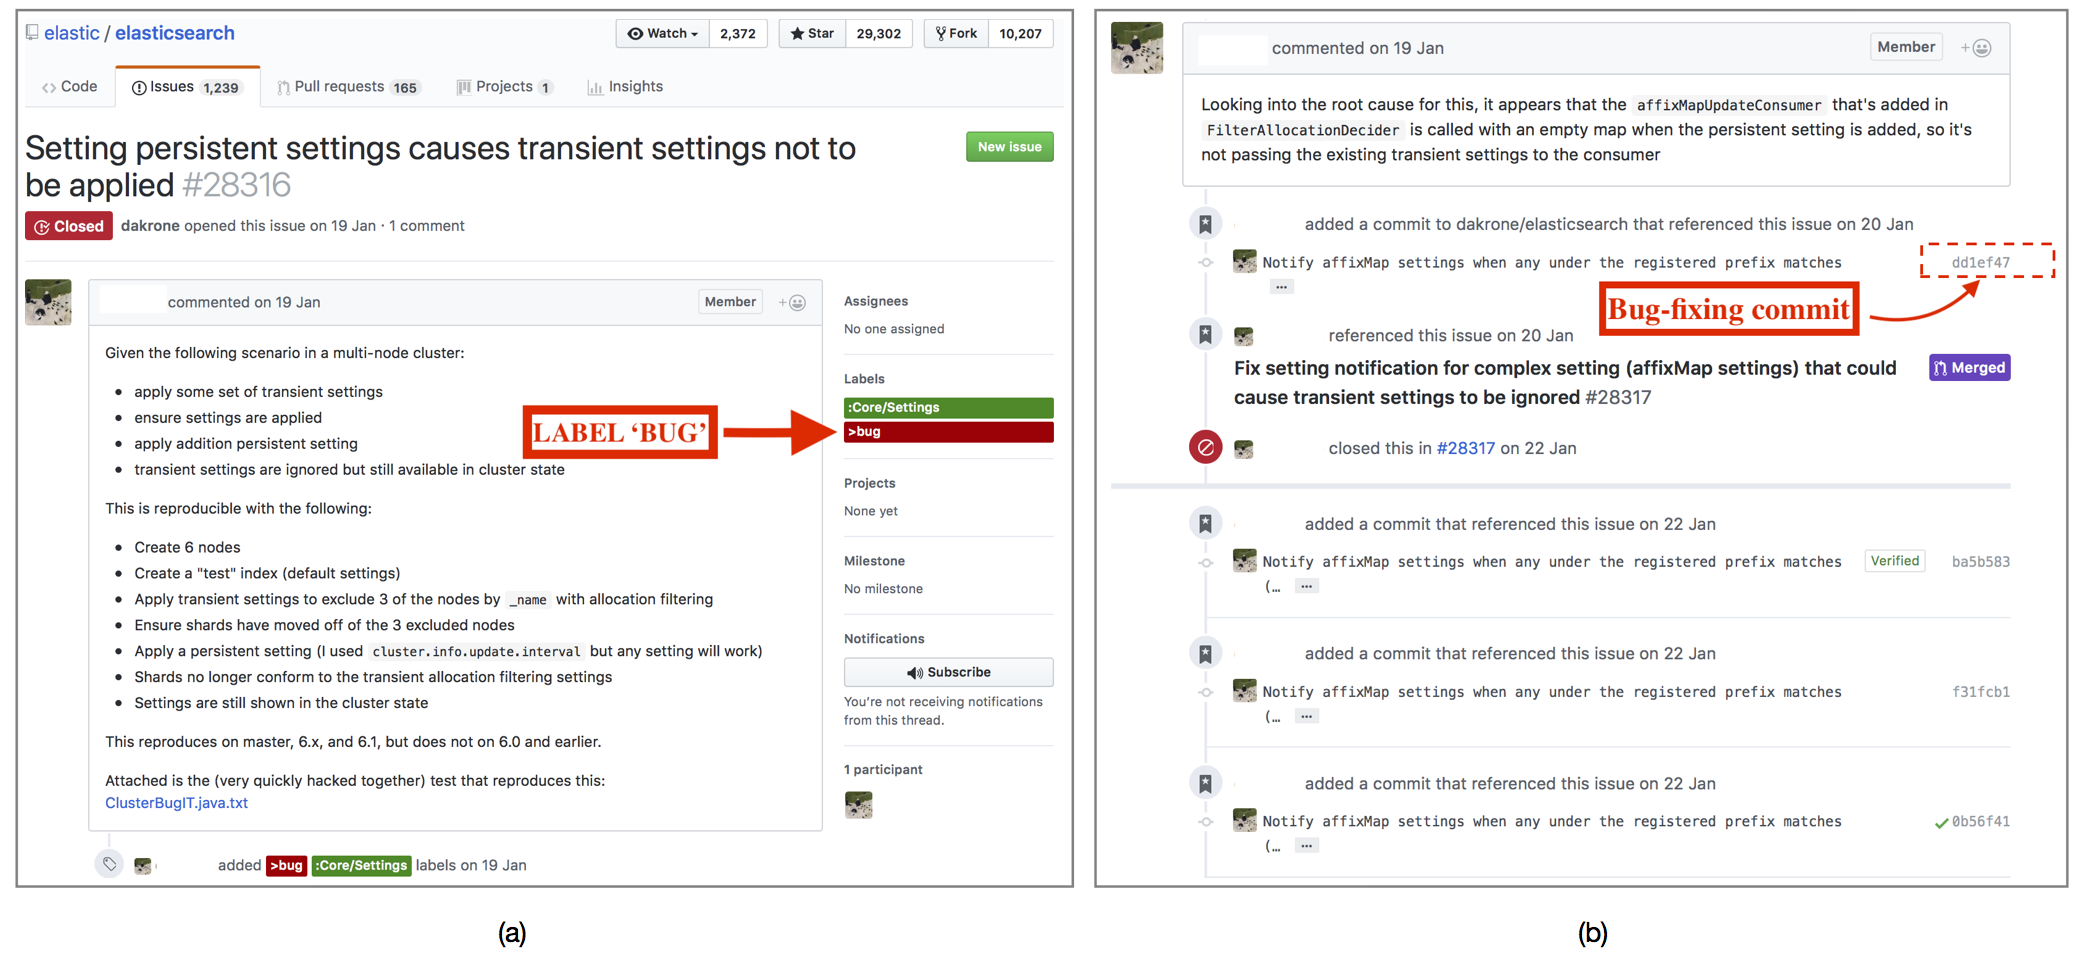
\includegraphics[width=\columnwidth]{img/bugreport.png}
\caption{Bug Report in ElasticSearch}
\label{fig:bugreport}       % Give a unique label
\end{figure}

Source code management systems also store the source code and their differences across different versions of the source code, they store metadata such as user-IDs, timestamps, and commit comments. This metadata explains who, how, when, and why the source code changed. Therefore by using this information and the information from the bug report, it is possible to understand which malfunction was caused by the bug, what problems in the source code were causing it, and how it was finally fixed.

Figure~\ref{fig:bugfix} \emph{(a)} shows the message of the commit that fixed the bug \emph{\#28316}\footnote{\url{https://github.com/elastic/elasticsearch/commit/ba5b5832039b591cfb00b8587966bd1f4ac28c40}}, this information is accompanied by the diff of the files that were modified to fix the bug in GitHub. Figure~\ref{fig:bugfix} \emph{(b)} shows the log entry of this Bug-Fixing Commit from the git repository of ElasticSearch project. This commit log can be obtained using the command \emph{git show} and the number of the commit. Git's log entry includes the author, date, and files involved in the change. Additionally, a text message describing the change is also recorded. This message is the same as the message on GitHub. 

\begin{figure}[ht]
\centering
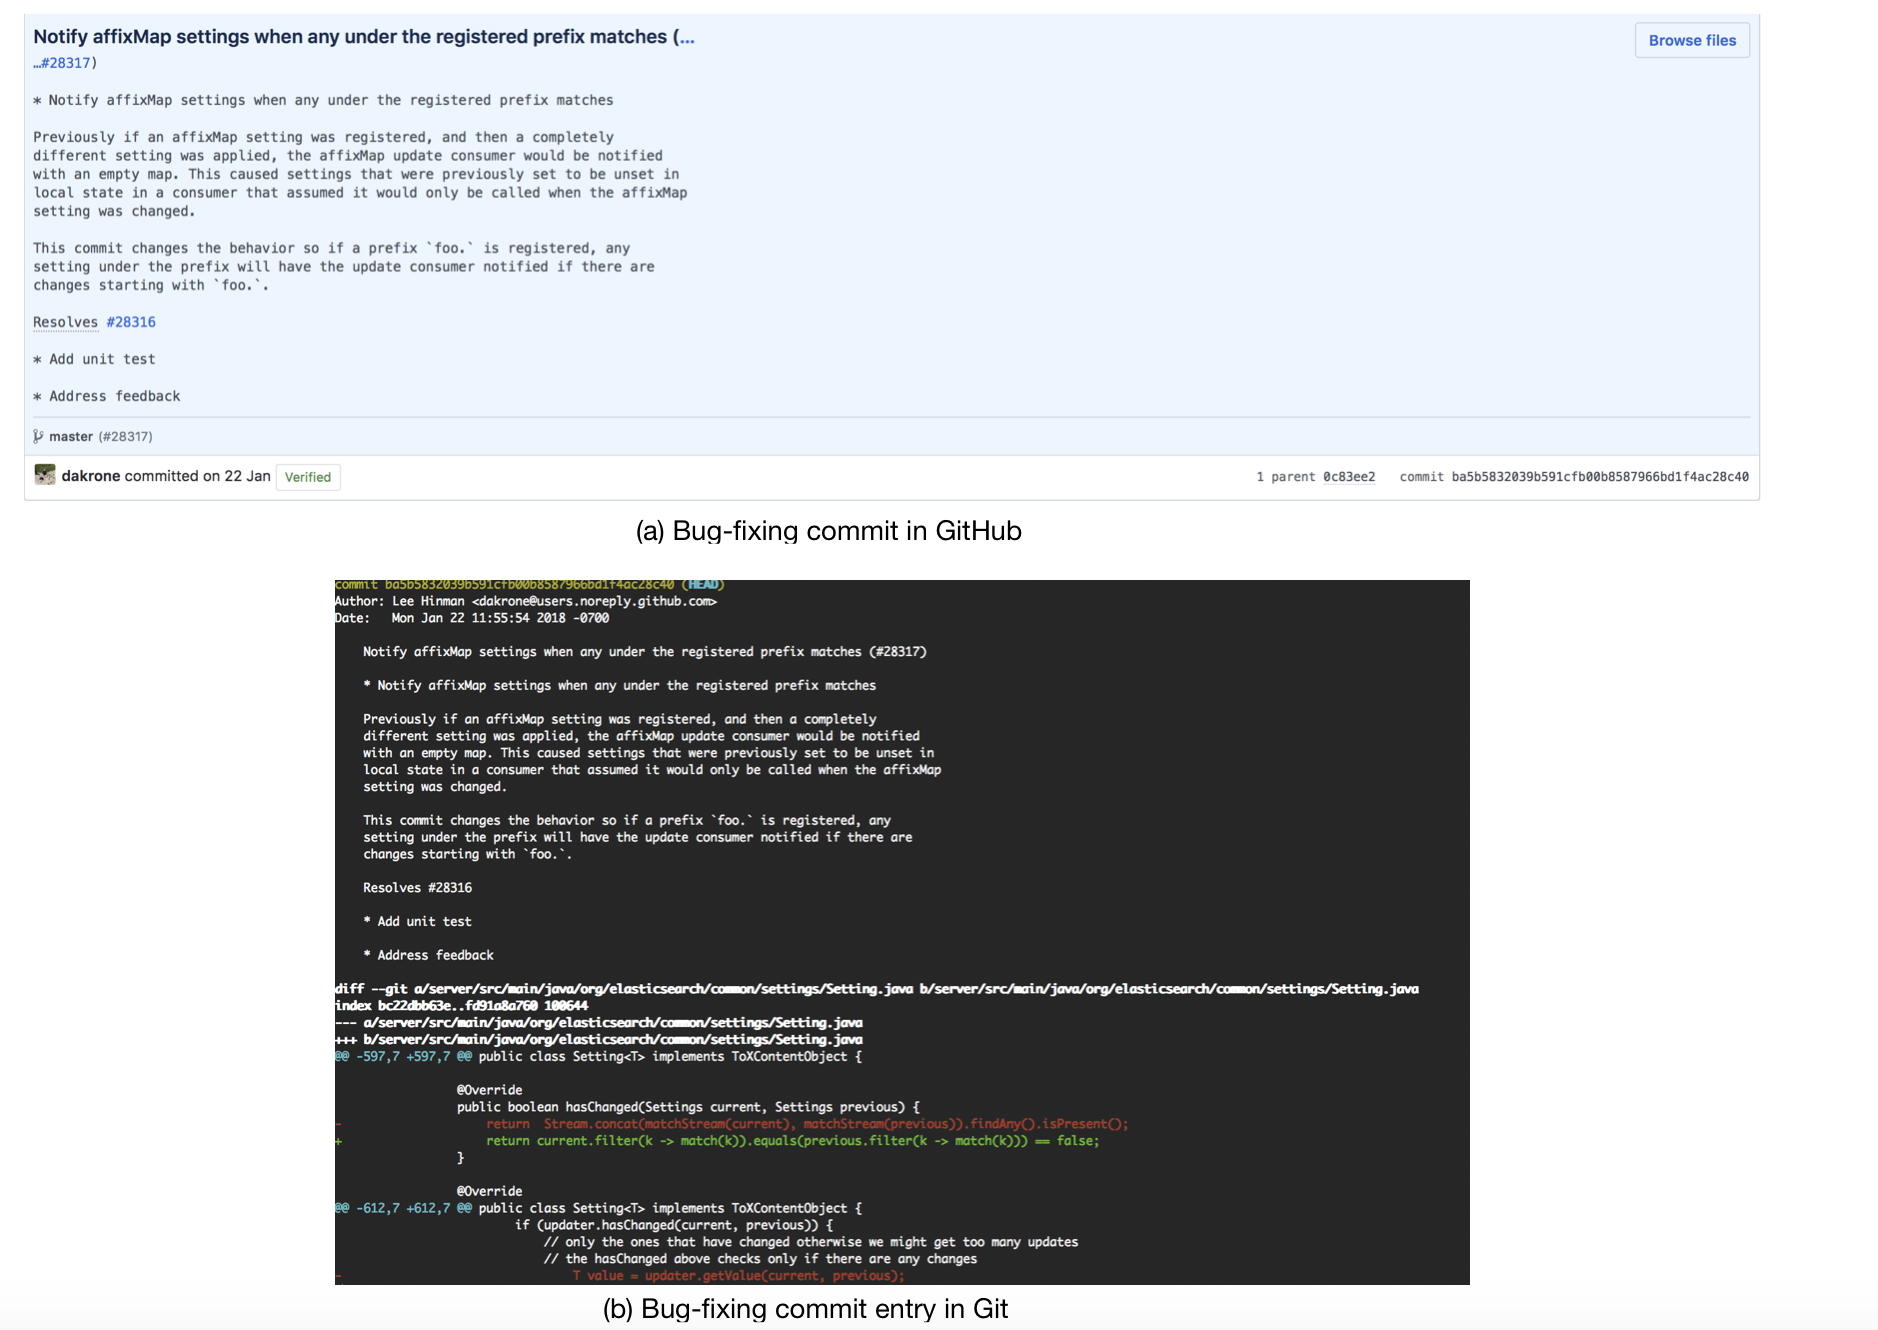
\includegraphics[width=\columnwidth]{img/bugfix.png}
\caption{Bug-Fixing Commit (\emph{ba5b5832039b591}) in ElasticSearch}
\label{fig:bugfix}       % Give a unique label
\end{figure}

With all these data, the history of a software component can be navigated to identify when a failure was occurring for the first time. Using the \FFC and \BIC, we might determine procedures to determine if given a bug reported and its corresponding fix which change was the first one to manifest the bug and which change inserted the buggy lines, and also whether both changes are the same or they differ.

%This way, we introduce the concept of ``first failing change" to extend the notion of ``introducing" (or ``seeding") a bu, as we commented before in the introduction. Using the \FFC, we might determine procedures to determine if given a bug reported and its corresponding fix, which change the first one to show a malfunction.

\subsection{SZZ algorithm}
\label{subsec:SZZintro}

In Software Engineering research, the SZZ algorithm~\cite{sliwerski2005changes} is a popular algorithm for identifying the origin of a bug~\cite{da2016framework,rodriguez2018reproducibility}. It was proposed by \'Sliwersky, Zimmermann, and Zeller in 2005 to identify the suspicious change to induce the later fix. The algorithm identifies the Bug-Fixing Commit, then uses a diff tool to compare the lines that differ between two revisions of the same file. In the SZZ, the authors assume that the lines that have been removed or modified in the Bug-Fixing Commit are the ones containing the bug. For this reason, SZZ traces back the lines through the code history (by means of the annotate/blame\footnote{Annotate is used in SVN and blame is used in Git} command), to find when the changed code was introduced.

Even though the algorithm addresses two different problems, it can be split into two main parts. The first part is related to the problem of linking to the VCS and the issue tracking system to identify the Bug-Fixing Commit. In this part, the algorithm identifies -by means of a set of heuristics- Bug-Fixing Commits through employing a technique that matches commits with bug reports labeled as fixed in the bug tracking system. Therefore, the algorithm uses regular expressions to identify bug numbers and keywords in the commit messages that are likely to point out a real bug fixing change.  The second part addresses the problem of identifying the Bug-Introducing Commit. In this part, the algorithm employs the diff functionality implemented in the source code management systems to determine the lines that have been changed (to fix the bug) between the fixed version and its previous version. Then, using annotate/blame functionality, SZZ is able to locate who modified or deleted those lines for the last time in previous commit(s), and, whether they were committed before. These change(s) are flagged as suspicious of being the Bug-Introducing Commit(s).

After the publication of this approach, two main areas in software engineering \emph{(SE)} were improved and deeply studied. The first area clearly includes studies related to the introduction of bugs~\cite{ pan2009toward,eyolfson2011time,asaduzzaman2012bug,bernardi2012developers,yangbug}. By studying Bug-Introducing Commits identified using the SZZ algorithm, researchers are able to correlate some characteristics of the software evolution of the project with time, such as the day that a change is recorded with the introduction of bugs~\cite{sliwerski2005changes}, the time between when a bug was reported and the moment it was inserted~\cite{rodriguez2017much} or even if developers are fixing their own bugs~\cite{izquierdo2011developers}. The second area includes studies that attempt to avoid the introduction of changes in the future based on the study of prior Bug-Introducing Commits. For example, avoiding bugs by using just-in-time (JIT) quality assurance practitioners and researchers build models that predict whether a change is likely to be a Bug-Introducing Commit before committing it into the source code~\cite{kim2008classifying,kamei2013large,kamei2010revisiting,nagappan2006mining}.

Despite being a fundamental algorithm in the community to locate the Bug-Introducing Commits, their results are limited. Firstly, there is not enough empirical evidence supporting the assumptions suggested by the SZZ, and the current evaluations are limited; Secondly, this algorithm fails in identifying the \BIC in some scenarios, i.e, when new lines in the Bug-Fixing Commits cannot be traced back, these types of commits are removed from the analysis. Thirdly, despite there are some studies facing challenges with this algorithm~\cite{kim2006automatic,williams2008szz,da2016framework}, all of them have the same assumption: `` The lines changed to fix a bug are the ones containing the malfunction''.

This thesis tries to shed some more light on how this algorithm performs in identifying the Bug-Introducing Commit through empirical evidence. Furthermore, the reason why algorithms such as the SZZ are failing to correctly identify which change caused the failure is studied further.

\section{Research goals}
\label{sec:goal}

Finding the cause of bugs has been an important topic during the last decades. The high importance and impact of this topic is an essential factor to understand and improve other areas related to bugs, such as bug detection, bug prevention, bug analysis and bug statistics. Many questions related to solving the problem of identifying the \BIC are proposed in this dissertation. All the bugs are not caused in the same way, and they do not present the same symptoms. Thus, they cannot be treated as equal when locating the cause of the bug.

\begin{figure}[ht]
\centering
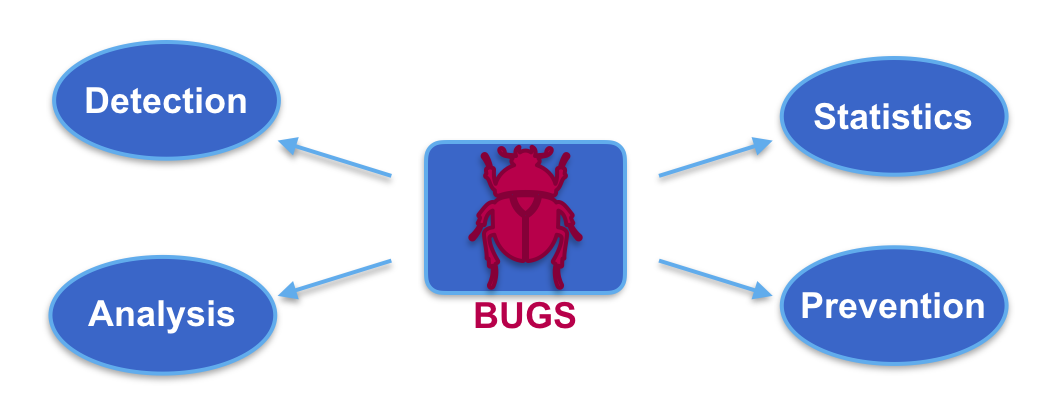
\includegraphics[width=\columnwidth]{img/SZZimportant.png}
\caption{Affected areas of studying the cause of a bug}
\label{fig:impact}       % Give a unique label
\end{figure}

There are many studies and approaches based on tracking back the lines of a Bug-Fixing Commit to locate the origin of bugs. Nevertheless, these approaches are not using any meaningful model that researchers might use to validate the ``real'' performance of the current state-of-the-art algorithms. These algorithms attempt to locate the line that ``contains the bug''. And researchers cannot be sure about the meaning of  ``injecting a bug'', because any previous study states the fact of introducing a bug, or the moment of when it was introduced. Consequently, researchers are not sure whether the bug was introduced in the moment of inserting the lines into the source code. For that reason, in this dissertation, we distinguish between bug manifestation moment (FFC) and the bug introduction moment (BIC). Because, it is possible that we have a \FFC without a BIC, for example, because of external resources. There is a moment when something has manifested itself but the reason is not related to the code, but it is related to a change in the environment.

To adress the lack of definitions and the need to validate the current algorithms. This thesis proposes a theoretical model to define which changes introduced bugs into the source code. This model assumes a perfect test which can be run indefinitely in the history of the project to find out when the failure was introduced and whether the change was responsible for the bug or it was something external. Furthermore, this model may be used as a framework to validate the performance of other approaches and researchers can compare the effectiveness of different algorithms. Setting this framework is one of the principal values of the thesis because the previous literature is not able to compute the ``real'' precision and recall of the current algorithms.

\section{Contributions}
\label{sec:contributions}

The main four contributions of this thesis are outlined below.
\begin{enumerate}
	\item\textbf{A Systematic Literature Review \emph{(SLR)} on the Use of the SZZ algorithm:} We have carried out a study to analyze reproducibility and credibility in Empirical Software Engineering~\emph{ESE} with the SZZ algorithm as case of study. The aim of the SLR is to obtain an overview of how authors have addressed the reproducibility and credibility in the studies where they have used the SZZ algorithm. This SLR has been published in the Information and Software Technology Journal in March, 2018 \cite{rodriguez2018reproducibility} and the goals of the study are described below:
	\begin{enumerate}
  		\item \textbf{An overview on the impact that the SZZ has had so far in ESE:} The SZZ algorithm has been shown to be a key factor to locate when a change introduced a bug. Furthermore, to provide insight of how widespread the use of SZZ is, we also addressed the maturity and diversity of the publications where SZZ has been used in order to understand its audience.
  		\item \textbf{An overview of how studies that use the SZZ algorithm address the reproducibility in their research work:} Reproducibility is a crucial aspect of a credible study in ESE~\cite{gonzalez2012reproducibility}. Piwowar et al. state that reproducibility improves the impact of research~\cite{piwowar2007sharing}. In addition, when a research work incorporates reproducibility, it is more likely to be replicated. However, there is evidence in the ESE literature that replicable studies are not common~\cite{robles2010replicating}. By providing a replication package, the authors facilitate others to replicate or to reproduce their experiment, which increases the credibility of their results~\cite{juristo2009using}.
 	 	\item \textbf{An analysis of how these studies manage the limitations of the SZZ algorithm:} Limitations of SZZ are well-known in the research literature, and we would like to analyze how many papers report any of the limitations or how they address them. Therefore, we study whether authors are aware of that and mention that some limitations of SZZ may affect their findings, be it in the description of the method, in the threats to validity or in the discussion.
	\end{enumerate}

	\item\textbf{A Theoretical Model to Unequivocally Identify the Bug-Introduction Changes:}
This dissertation describes a comprehensive model to identify how bugs are introduced into the source code. This model includes a set of definitions which formally helps to analyze the process. Furthermore, it also includes an exploratory taxonomy that helps in understanding how a bug is introduced and manifested into the source code. 

	The goals of the model are:
	\begin{enumerate}
 		 \item \textbf{A detailed definition of the Bug-Introducing Change and the First-Failing Change:} The model introduces a general method to determine, unequivocally and falsifiability, the first time that the software fails in relation with the bug-fixing change, identifying the \BIC when it exists.
 		 \item \textbf{The criterion to apply the model:} The model relies on the existence of a hypothetical test that can be run indefinitely in each past version of a project to check whether or not the code was buggy at this point. Since the hypothetical test is not automatized, the criterion describes how it should be run and the possible outcomes after applying it. 
 		% \item \textbf{The fundamentals to compute false/true positives and false/true negatives:}
	\end{enumerate}

	\item\textbf{Empirical Study on the Application of the Proposed Model:}
	This dissertation presents an empirical study of the proposed theoretical model. This study analyses the publicity of available data sources from two open source software projects, Nova and ElasticSearch and describes a model to identify unequivocally the bug introduction commit or to determine whether it exists given a Bug-Fixing Commit. 
	The goals of the empirical study are:
	
	\begin{enumerate}
		\item \textbf{The frequency of \BFC induced by \BIC in Nova and ElasticSearch:} The empirical study manually identifies whether a \BFC was induced by a \BIC, or whether other reasons may explain the cause of the failure. Thus, the frequency of a \BIC being induced by a \BIC in the two cases of study can be computed.
		
 		\item \textbf{The ``gold standard'' dataset:} The proposed model enables to define the ``gold standard'' to be defined where commits in the repositories are BIC. This dataset favors the comparison with the performance of some state-of-the-art approaches to computes the ``real''  false positives and false negatives.  
	\end{enumerate}

	\item\textbf{Quantification of the SZZ Algorithm:}
This thesis studies and contextualizes the current problem of identifying a Bug-Introducing Commit given a Bug-Fixing Commit using algorithms based on tracking back the lines that were modified to fix the bug. Furthermore, there is quantification of the possible sources of error when identifying the Bug-Introducing Commits using the SZZ algorithm or some variants of it. Since the thesis defines the ``gold standard'', we can compute the ``real'' performance of the SZZ algorithm when identifying the Bug-Introducing Commits because we are sure of the ``real'' true positives and true negatives in their results.
\end{enumerate}

\section{Structure}
\label{sec:structure}

The remainder of this thesis is organized as follows. %This chapter has depicted an overall idea of importance to distinguish the \BIC and the \FFC in the study of the bug seeding process. Specifically, it focuses on explaining the bug seeding activity, describing the version control system and detailing one of the most used algorithms for identifying the commit that introduced the bug.

Chapter~\ref{chap:stateoftheart} provides a detailed description of the current state of the art to the reader. Then, Section~\ref{sec:bugSeedingBG} mentions some studies in the filed of bug seeding and bug location. Finally, Section~\ref{sec:SZZuse} details some bibliography related to the SZZ algorithm.

Chapter~\ref{chap:context} addresses the current problem to identify the first moment when the system fails by providing motivating examples and explaining the reasons why algorithms sometimes fail when locating the Bug-Introducing Commits. Furthermore, this Chapter explains the role of the VCS in the bug seeding activity.

Chapter~\ref{chap:credibility} discusses the reproducibility and credibility of the studies that used the SZZ in the ESE. This Chapter draws an overview of the impact that this algorithm has in the ESE community and how researchers use it in different fields to identify the \BIC.

Chapter~\ref{chap:Theory} contains a detailed description of our proposed approach to deal with the inaccurate algorithms to locate the moment when the bug manifest the failure by the first time. This theoretical model allows for a better framing of the comparison of automatic methods to find Bug-Introducing Changes. This model may distinguish between the bug introduction moment and bug manifestation moment. 

Chapter~\ref{chap:application} applies the proposed theoretical model into two cases of study: ElasticSearch and Nova. Both projects are open source projects with many thousand of actives developers. Section~\ref{sec:methodology} describes the methodology used in the studies to explain how manually identify the bugs that were injected into the source code by navigating back into the lines of code that were modified in the Bug-Fixing Commit to fix the bug. Finally, Section~\ref{sec:results} presents the results of the empirical study after applying the theory of bug introduction. 

Chapter~\ref{chap:discussion} details the threats to validity of this dissertation in Section~\ref{sec:threats} and then it discusses each of the results obtained in this thesis in Section~\ref{sec:discussion}.

Finally, Chapter~\ref{chap:conclusions} draws some conclusions and concludes with the potential further work to be done.

%Moreover
%Pareto phenomenon
%Who should resolve the bugs?
% Someone who had similar bugs in the past!
%A bug you like: A framework for automated assignment of bugs
%Reducing the effort of bug report triage: Recommenders for development-oriented decisions
%Automatic bug triage using semi-supervised text classification
%An empirical study of the integration time of fixed issues

%Tangled commit also introduced more noise to locate the BIC, but with the \FFC we do not concerned about them, because we these modifications are not in the 'test' that we want to pass to previous versions "The Impact of Tangled Code Changes (paper to read)" %%%%%%%%%%%%%%%%%%%%%%%%%%%%%%%%%%%%%%%%%%%%%%%%%%%%%%%%%%%%%%%%%%%%%%%%%%%%%%%%
%%%%%%%%%%%%%%%%%%%%%%%%%%%%%%%%%%%%%%%%%%%%%%%%%%%%%%%%%%%%%%%%%%%%%%%%%%%%%%%%
% BACKGROUND %
%%%%%%%%%%%%%%%%%%%%%%%%%%%%%%%%%%%%%%%%%%%%%%%%%%%%%%%%%%%%%%%%%%%%%%%%%%%%%%%%

\cleardoublepage
\chapter{State of the art}
\label{chap:stateoftheart}

This chapter outlines an overall picture of the bug life cycle, bug seeding and bug location process in the Software Engineering~\emph{(SE)}. The information from the bug seeding process may be used in other areas of~\emph{SE} such as bug prediction,  bug triage or software evolution.  This chapter describes the related work necessary to understand how this thesis fits into the current literature. It explains the life cycle of a bug and the research works that other authors have carried out to locate the cause of bugs.

\section{Bug Life Cycle}
\label{sec:buglife}
In this section the mian focus is on understanding a the bug's life cycle. Sommerville ~\cite{sommerville2010software} claims that it is not possible to avoid the unintentional introduction of bugs in the source code because it is inherited in the process os software making. To help with this process, several tools and product quality have been developed in order to reduce the number of bugs and improve the software development process.

Generally, the open source projects leave the management of issues to specific tools such as the Bug Tracking System. The open source systems studied in this dissertation uses Launchpad and GitHub as their Bug Tracking System, although the best-known bug tracking system is Bugzilla\footnote{ww.bugzilla.org/}. For example, in Bugzilla the life of a bug starts when a developer or user detects a wrong behavior and reports it to the system. The initial status of the report is UNCONFIRMED. Developers legitimatize the status by reproducing the symptoms described in the report where it is confirmed, meaning that the bug is real. The status is changed to NEW, and the bug is considered open from here onwards. An open bug's status is changed to ASSIGNED once it is assigned to a developer for fixing. The status of a bug changes to RESOLVED when its resolution is either: FIXED, DUPLICATE, WONT-FIX, WORKSFORME, INVALID, REMIND, LATER. Next, a Quality Assurance (QA) person might verifies the resolution by either accepting it or rejecting it, turning the outcome to either VERIFIED or REOPEN. Finally, when a bug is labeled as VERIFIED it can be marked as CLOSED which concludes the bug resolution process. Although the steps above describe the common process of a bug, there are other possible paths in the life cycle of a bug.

During this cycle, the developers and users might discuss about the possible cause of the bug or the reason why the project manifests the failure. Thus, the greater the understanding of a bug's life cycle, the greater the explanation of the root cause.

\subsection{Characteristics of bugs}
\label{subsec:characteristics}
With this respect, previous works have studied bug characteristics in large software systems~\cite{chou2001empirical,gu2003characterization,ostrand1984collecting,ostrand2002distribution,podgurski2003automated, sullivan1992comparison,chen2014empirical,li2006have,beizer2003software,tan2014bug}. Recent papers  performed empirical studies to characterize and classify the bugs in open source software depending on the different challenges that arise in the bug finding process. Lu~\emph{et al,.} classified bugs in three categories depending on their root cause: Semantic, Concurrency, and Memory~\cite{lu2005bugbench}. Then, Li Tan~\emph{et al,.} extended the previous root cause classification by adding more cases, while also introducing two more dimensions, Impact and Software Component \cite{tan2014bug}. Table~\ref{tab:dimensions} shows how the root cause is related with the fault, the impact is related with the failure caused by the bug, and lastly, the component is related with the location of the bug~\cite{li2006have}. Finally, Chen~{et al.,} included additional sub-categories after manually studying how bugs  are introduced in a version of the software system, but they are not found until much later affects the quality of software systems ~\cite{chen2014empirical}. Assadollah~{et al.,} proposed a detailed classification of bugs depending of its root cause: memory related bugs, concurrent bugs and semantics bugs.

\begin{table*}
\centering
\newcommand{\specialcell}[2][l]{%
  \begin{tabular}[#1]{@{}l@{}}#2\end{tabular}}
% increase table row spacing, adjust to taste
\renewcommand{\arraystretch}{1.3}
\caption{Bug categories of the three dimensions: Root Cause, Impact, and Component}
\label{tab:dimensions}

\begin{tabular}{lll}
\toprule
\textbf{Dimension}& \textbf{Subcategory}& \textbf{Description} \\
\midrule
\multirow{3}{*}{Root Cause}&Memory & Improper handling of memory objects. \\
&Concurrency & Synchronization problems\\
& Semantic & \specialcell{Inconsistencies with requirements or \\programmers' intention}\\
 \hline
 \multirow{6}{*}{Impact}& Hang & Program keeps running but does not respond.\\
    & Crash&Program halts abnormally.\\
    & Data Corruption&Mistakenly change user data.\\
    & Perfor. Degradation& Functions correctly but runs/responds slowly.\\
    & Incorrect functionality&Not behaving as expected.\\
    &Other&other impacts.\\
 \hline
 \multirow{4}{*}{Software Component}& Core& Related to core functionality implementations.\\
 &GUI &  Related to graphical user inter- faces.\\
 &Network&Related to network environment and communication.\\ 
 &I/O& Related to I/O handling.\\
 \bottomrule
\end{tabular}
\end{table*}


\begin{table*}
\centering
\newcommand{\specialcell}[2][l]{%
  \begin{tabular}[#1]{@{}l@{}}#2\end{tabular}}
% increase table row spacing, adjust to taste
\renewcommand{\arraystretch}{1.3}
\caption{Categories of root causes of bugs found in \cite{asadollah2015towards,chen2014empirical,lu2005bugbench}}
\label{tab:rootcause}

\begin{tabular}{lll}
\toprule
\textbf{Category}& \textbf{Subcategory} & \textbf{Description} \\
\midrule
\multirow{7}{*}{Concurrency}&Data race&Two or more threats access to write the same data\\
&Atomicity-related& A concurrent overlapping execution between two sequences\\
& Deadlock & A process depend by another process to proceed\\
& Order Violation&Violation of the desired order\\
& Livelock& A thread is waiting for an unavailable resource\\
& Starvation& A process indefinitely delayed \\
&Suspension&A calling thread waits for a long time\\
 \hline
 \multirow{6}{*}{Memory}& NULL Pointer Dereference & Dereference of a null pointer\\
    & Memory leak &Failures to release unused memory \\
    &Uninitialised Memory Read & Read memory data before it is initialized\\
    &Dangling Pointer & Pointers still keep freed memory addresses\\
    &Overflow & Illegal access beyond the buffer boundary\\
    &Double Free & One memory location is freed twice\\
 \hline
 \multirow{10}{*}{Semantic}& Missing Cases&A case in a functionality that is not implemented\\
 &Missing Features&A feature that is not implemented\\
 &Corner cases&Incorrect or ignored boundary cases\\ 
 &Wrong control flow&Incorrect implementation of sequences of function calls\\
 &Exception handling & Do not have proper exception handling\\
 &Processing &Incorrect Evaluation of expressions/equations \\
 &Typo & Typographical mistakes \\
 &Design Issue & Incorrect Design or API/function\\
 &Incorrect Documentation & \specialcell{Incorrect/inconsistent documentation of \\software and source code}\\
 &Other & Any other semantic bug\\
\bottomrule
\end{tabular}
\end{table*}

Many authors have used this classification to deal with different purposes regarding automatic approaches for software bug classification, as well as empirical and methodological studies on the case of software errors, taxonomic studies for software bugs and the study of bug characteristics in the OSS. Vahabzadeh~\emph{et al,.} attempts to understand the characteristics of bugs in test code. In this study the authors also insert  the \emph{Environment} category when referring to tests that pass or fail depending on the operating system and the incompatibilities between different versions of JDK. They discovered that incorrect and missing assertions are the main root cause of dormant bugs\cite{vahabzadeh2015empirical}. Jeffrey~\emph{et al,.} developed a technique to automatically isolate the root cause of memory-related bugs; their approach is effective in finding root causes when memory corruption propagates during execution until a failure crash occurs\cite{jeffrey2008identifying}. Wan~\emph{et al,.} studied 1,108 bug reports in order to understand the nature of the bug, they also introduced other categories such as \emph{Security}, \emph{Environment and Configuration}, \emph{Build}, \emph{Compatibility} and \emph{Hard Fork}. Their findings indicate that security bugs take the longest median time to be fixed, and also that the environment and configuration bugs are one of the major types of bugs along with the semantic bugs \cite{wan2017bug}. 

%\gema{quiza hablar un poco mas de este estudio}
%\gema{anadi andy works abou enviromental CI ms paper 2017}

On the other hand, some authors have also considered using other characteristics to classify bugs. Sahoo~\emph{et al,.} used the reproducibility of a bug, the observed symptoms and the number of inputs needed to trigger the symptom to distinguish between deterministic, time dependent or non-deterministic bugs \cite{sahoo2010empirical}. Chandra and Chen distinguished environment-dependent  from environment-independent bugs in the Apache, GNOME, and MySQL \cite{chandra2000whither}. Zhang~\emph{et al,.} computed the bug fixing time and identified factors that influence it on three open source software applications. They found the assigned severity, the bug description, and the number of methods and changes in the code as impacting factors.

\section{Bug Seeding and Bug Location}
\label{sec:bugSeedingBG}

To locate the origin of bugs, researchers have proposed two different procedures. Some researchers use techniques starting with a Bug-Fixing Commit in order to identify the most recent commit(s) that was changed to fix the bug. Other researchers use techniques to locate root causes of software failures by analyzing program traces. These approaches do not rely on identifying the Bug-Fixing Commit, instead they attempt to find an association between program failures and the execution of program elements.

In this section, the state of the art processes for identifying the Bug-Fixing Commits as well as Bug-Introducing Commits are discussed. Although this thesis is mainly motivated in the techniques that uses the Bug-Fixing Commit to identify the commit that caused the bug, other existing and popular techniques are also discussed.

\subsection{Identifying the Bug-Fixing Commit}
\label{subsec:identifyBFC}

Previous works have attempted to identify Bug-Fixing Commits in version archives. Mockus and Votta performed an analysis to identify the reasons for software changes using historic databases; they used the textual description in the log of a commit to understand why the change was performed~\cite{mockus2000identifying}. Cubrani\'c and Murphy recommended a practice that uses a bug report number in the comment when the practitioners fix a bug report, thereby linking the changes with the bugs~\cite{vcubranic2003hipikat}. Finally, \'Sliwersky~\emph{et al.} proposed the~\emph{SZZ} algorithm that links a version archive to a bug database in order to automatically identify and analyze fix-inducing changes~\cite{sliwerski2005changes}; the authors made use of the previous work mentioned before, and also benefited from Fischer's~\emph{et al.} work in which they proposed a technique to identify references to bug databases in log messages, then used these references to infer links from VCS archives to BUGZILLA databases~\cite{fischer2003analyzing,fischer2003populating}. In summary, the SZZ automatically links change logs and bug reports using some heuristics which search for specific keywords (such a `` Fixed'' or ``Bug'') and bug IDs (such a ``\#1234'') in change logs \cite{bachmann2009software,mockus2000identifying,schroter2006if,zimmermann2007predicting}. This heuristic relies on `` developers leaving hints or links regarding bug fixes in the change logs''~\cite{wu2011relink}. 

However, the quality of the change logs are not ensured as they may incorrectly link with the Bug-Fixing Commit from the version archives with issue reports that are not bug reports from the issue tracking system. Bird~\emph{et al.} discovered that the absence of bug references in change logs affected the number of missing links leading to biased defect information, thereby affecting defect prediction performance \cite{bird2009fair}. Researchers have further investigated this misclassification during the past years as the heuristics might yield biased data, Bird and Bachmann et al. confirmed this problem and reported that 54\% of bug reports are not linked to Bug-Fixing Commits \cite{bachmann2010missing,bird2009fair}. Bettenburg~\emph{et al.}  noticed that the issue reports often present incomplete and incorrect information \cite{bettenburg2008makes}. Antoniol~\emph{et al.} noticed that many of the issues in issues tracking systems did not describe bug reports \cite{antoniol2008bug}. Herzig~\emph{et al.} found that around one third of the bug reports that they manually analyzed were not describing a bug \cite{herzig2013s}. Nguyen~\emph{et al.} showed that even in a near-ideal dataset, the biases exists \cite{nguyen2010case}.

On the other hand, some researchers have attempted to mitigate the limitations and shortcomings of linking bug reports with Bug-Fixing Commits \cite{herzig2013s,rodriguez2016bugtracking,tan2015online}. Thus,  practice, tools and algorithms have been developed in order to mitigate this problem. For instance, GitHub supports linkage by automatically closing issues whether the commit message contains the \emph{\#numberOfIssue}, many Free/Open Source Software projects have adopted as a good practice to use keywords in their commit comments such as ``\# fix-bug -'' when they are fixing a bug, as it has been reported for the Apache HTTP web server7 in \cite{bachmann2010missing}, and for VTK8, and ITK9 in \cite{mcintosh2016empirical}. In addition, several authors have suggested the used of semantic heuristics \cite{schroter2006if,vcubranic2003hipikat,zimmermann2007predicting}, while others have proposed solutions that rely on feature extraction from bugs and issue tracking system metadata. For Instance, Wu~\emph{et al.} developed ReLink to automatically link bugs reports and commits based on the similarity between the texts in both \cite{wu2011relink}. Bird~\emph{et al.} suggested manual inspections by developers in order to identify missing links. They proposed the tool LINKSTER that helps developer to locate possible links by providing query interfaces to the data \cite{bird2010linkster}. Nguyen~\emph{et al.} proposed the Mlink tool to mitigate some of the problems found in ReLink, for instance some code changes in the commit are excluded and both issue reports and commit are used as plain texts \cite{nguyen2012multi}. Le~\emph{et al.} continued working on the shortcomings of the previous tools and develop RCLinker, which enriches commit logs. This approach extracts textual and metadata features from issues and commits \cite{le2015rclinker}. As a consequence of these efforts, the linkage problem has been addressed and its accuracy has drastically increased. For example, FRlink, an existing state-of-the-art bug linking approach, has improved the performance of missing link recovery compared to existing approaches, and it outperforms the previous one by 40.75\% (in F-Measure) when achieving the highest recall \cite{sun2017frlink}.

\subsection{Identifying the Bug-Introducing Commit}
\label{subsec:identifyBIC}

Failure-inducing\footnote{Notice that some authors use failure-inducing as the concept for bug-introducing} changes were first addressed by Ness and Ngo in 1997~\cite{ness1997regression}. They described how to identify a single failure-inducing change using simple linear and binary search. Their goal lies in isolating failure-inducing changes by applying chronological changes to a program until the fixed version presents the same wrong behavior as the next version of the program. Despite this, the technique is able to reduced the computational cost of testing each combination of changes introduced in the faulty version to locate the failure-inducing changes. However, this technique fails when instead of one change, a set of changes cause the failure. To deal with the issue, Zeller proposed the automated delta debugging technique, which can determine the minimal set of failure-inducing changes by gradually increasing granularity to identify the differences (that is, the deltas) between a passing and a failing subset~\cite{zeller1999yesterday}.

Purushothaman and Perry~\emph{et al.} measured the likelihood for small changes, particularly one-line changes, to introduce errors. They refer to fix-inducing changes as~\emph{dependencies} which are changes to lines of code that were changed by an earlier commit. They assume that if the latter change was a bug fix, the original change was erroneous. The study concludes that the probability of a one-line causing a bug to be less than 4\%~\cite{purushothaman2004towards}. Baker and Eick also used a similar concept when referring to fix-inducing changes,\emph{fix-on-fix changes}. However, this concept requires both changes to be fixes. The paper describes a graphical technique for displaying large volumes of software where directories and subdirectories with high fix-on-fix rates were identified~\cite{baker1994visualizing}.

\paragraph{When a Bug-Fixing Commit exists:}

As previously mentioned, \'Sliwersky~\emph{et al.} proposed by first time an algorithm, the SZZ, that locates fix-inducing changes in version archives~\cite{sliwerski2005changes}. Although the SZZ algorithm provides a technique to identify possible  Bug-Introducing Commits, it has to deal with the incorrect identification of bug-inducing changes. For this reason, many efforts have been made to suggest improvements to the SZZ algorithm. First, Kim~\textit{et al.} developed an algorithm that automatically identifies  Bug-Introducing Commits; the algorithm is based on improvements of the SZZ algorithm that remove false positives and negatives by using the \textit{annotation graph} technique instead of using VCS \textit{annotate} to locate the lines changed in the bug-fixes. With this modification, the SZZ may avoid some false positives by not considering 
non-semantic source code changes, (i.e. blank spaces, changes in the format or changes in the comments) and by ignoring outlier fixes. After a manual validation, the new version of SZZ can remove about 38\%-51\% of false positives and 14\%-15\% of false negatives~\cite{kim2006automatic}. Secondly, Williams and Spacco proposed another enhancement of the SZZ algorithm. The authors suggested to use a mapping algorithm instead of the annotation graphs because they are more precise when facing larger blocks of modified code in bug fixes; this new approach uses weights to map the evolution of a unique source line and ignores comments and formatting changes in the source code with the help of \texttt{DiffJ}, a Java-specific tool. The authors also verified how often the  Bug-Introducing Commits were the true source of a bug in a small sample size, where 33 of 43 lines mapped to a bug fix showed evidence of a bug being introduced~\cite{williams2008szz}. Then, Da Costa~\textit{et al.} realized that during the last ten years there was not much research conducted to evaluate the results of the SZZ, they proposed a framework that evaluates the results of the different SZZ implementations based on a set of criteria such as the earliest bug appearance, the future impact of changes, and the realism of bug introduction. Their findings suggest that the previous SZZ enhancements tend to inflate the number of incorrectly identified  Bug-Introducing Commits, and by using this framework, the practitioners can evaluate the data generated by a given SZZ implementation and they might eliminate unlikely  Bug-Introducing Commits from their outcome~\cite{da2016framework}. Campos Neto~\textit{et al.} worked on improving the SZZ algorithm by disregarding refactoring changes as the  Bug-Introducing Commits because they do not change the system behavior. The authors empirically investigated the impact of such refactoring in both changes, bug-fixing and bug-introducing. Their results indicate that their approach can reduce 20.8\% of the incorrect  Bug-Introducing Commits when compared to the first SZZ approach \cite{neto2018impact}.

Other authors have created new approaches based on the same concept as SZZ algorithm, by attempting to mitigate the incorrect identification of  Bug-Introducing Commits. Kawrykow and Robillard developed \emph{DiffCat}, a tool-supported technique to detect and remove non-essential changes in the revision histories of projects. Their findings showed that up to 15.5\% of system's method updates consisted entirely of non-essential modifications, \cite{kawrykow2011non}. Ferdian~\textit{et al.} looked at the root cause of the bugs by applying a combination of machine learning and code analysis techniques, then verifying their approach through comparing the results with their manual analysis of 200 bug reports. This approach identifies the erroneous lines of code that cause a chain of erroneous behavior in the program leading to the failure; it has a precision of 76.42\%, and a recall of 71.88\% \cite{thung2013automatic}. Servant and Jones introduced the fuzzy history graph; this technique helps to represent the code lineage as a continuous metric providing a balance of precision and recall. This technique performs better over the evolution of the code when compared to other models \cite{servant2017fuzzy}.  

Other techniques are related to dependence techniques. These approaches also attempt to locate the Bug-Introducing Commit; they address some of the shortcomings in the text-based approaches by examining the behavior of the changes by using a program dependence graph (PDG). Dependence-based techniques compare the PDG for the bug-fixing change to the PDG for the previous version. First, PDG only identifies removed dependencies, it only examines added dependencies when no dependencies were removed and returns only the most recent version involved. Sinha~\textit{et al.} introduced this technique in order to identify the Bug-Introducing Commit by analyzing the effects of Bug-Fixing Commit on program dependencies. This is a significant improvement over the text approach used by the SZZ algorithm, as this approach takes into account semantics of code changes, similar to previous work \cite{horwitz1990identifying, binkley1992using}. This make the approach to be more accurate and applicable to a wider class of bug-fixing changes (i.e., changes that involve addition of statements). Their results increased the precision and the recall of the fixes by 19\% and 15\% when compared to the text approach~\cite{sinha2010buginnings}.  After this technique was introduced, many additions and refinements were made. Davies ~\textit{et al.} compared text-based and dependence-based techniques for identifying bug origins. The authors suggested detailed improvements to identify bug origins by combining both techniques \cite{davies2014comparing}. 

\paragraph{When a Bug-Fixing Commit do not exist:}

Contrary to the previous authors, some authors have studied the origin of bugs  without identifying the Bug-Fixing Commit;  and they have developed different methods such as Delta Debugging \cite{misherghi2006hdd,zeller2002simplifying,cleve2005locating,zeller2002isolating}, Spectrum Based Fault Location \cite{reps,janssen2009zoltar,harrold2000empirical,tiwari2011spectrum,abreu2007accuracy,jones2002visualization}, Nearest Neighbor \cite{renieres2003fault,jones2002visualization,abreu2007accuracy}, set union and set intersection \cite{}.A brief description of each method is given as follows. 

\emph{Delta Debugging} Zeller and Hildebrandt described the Delta Debugging algorithm for the first time in ~\cite{zeller2002simplifying}. This algorithm compares the program states of a failing and passing run, while using binary search with iterative runs. The iterations stop when the smallest state change that caused the original failure is identified.  In other words, this technique defines a method to automatize the process of making different hypotheses about how changes affect output to locate failure causes.  Gupta~\textit{et al.} used Delta Debugging combined with dynamic slicing to identify the set of statements that is likely to contain a faulty code~\cite{gupta2005locating}. Cleve and Zeller~\cite{cleve2005locating} presented the Cause Transitions technique and compared it to the Nearest-Neighbour technique. Their results suggest that, on the same set of subjects, Cause Transitions technique performs better than Nearest Neighbour.

\emph{Spectrum Based Fault Location}: A method used to locate faults from the identification of the statements involved in failures was first introduced in~\cite{reps}. This technique usually takes as inputs two sets of spectra, one for successful executions and the other for failed executions. It reports candidate locations where causes of program failures occur (e.g., lines, blocks, methods, etc.), which may be presented to debuggers. There are many spectra such as node spectra, edge-pair spectra, edge spectra and block spectra. Jones~\textit{et al.} developed the Tarantula system which provides a way to rank statements in terms of their likelihood of being faulty. Furthermore, it has a graphical user interface that specifies a color for each statement in the program depending on the suspiciousness of being buggy\cite{jones2002visualization}. Abreu~\textit{et al.} investigate the diagnostic accuracy of the spectrum-based fault localization as a function of several parameters using the Siemens Set benchmark. Their results indicate that the superior performance of a particular coefficient is largely independent on test case design~\cite{abreu2007accuracy}.

\emph{Nearest Neighbour}. Renieres and Reiss used Nearest Neighbour queries to locate the fault~\cite{renieres2003fault}. This technique contrasts a failed test with a successful test which in terms of distance, is more similar to the failed test. It uses these two test cases to remove the set of statements executed by the passed test case from ones executed by the failed test case. A bug is then located whether it is in the difference set between the failed run, and its most similar successful run. In case the bug is not contained in the difference set, this technique continues constructing a program dependence graph, while adding and checking adjacent un-checked nodes in the graph until the bug is located. This method is easily applicable since it only requires a classification of the runs as either incorrect or faulty from the users.

\emph{Set union and Set intersection}
The set union computes the union of all statements executed by passing test cases and taking these from the set of statements executed by a failing test case. The suspicious statements are contained in the resulting subset of all coverage entities that the user must explore. While this is happening, the set intersection computes
the set difference between the set of statements that are executed by every passed test case and the set of statements that are executed by a single failing test case. A set of statements is obtained by intersecting the set of statements executed by all passed test cases and removing the set of statements executed by the failed test case. %\gema{rephrase it} 


%- Micro interaction metrics (MIMs) that leverage developers' interaction information (Micro Interaction Metrics for Defect Prediction)

\paragraph{Tools for locating bugs:}

A lot of effort have been made to develop practical tools that assist in locating and detecting the bugs. Without trying to be exhaustive, a brief description of some tools that have been used to find bugs in the source code is given.

FindBugs\footnote{http://findbugs.sourceforge.net} is an automatic detector for bugs with the same pattern in Java source code.  The user experience of this tool showed that it was helpful and most of the warnings fixed in a specific organization were ``hashcode/equals problems, serialization issues, unchecked method return values, unused fields and constants, mutable static data, and null pointer dereferences''~\cite{hovemeyer2004finding}. HATARI is a plugin for Eclipse that determines how risky is a change depending on the area of source code\cite{sliwerski2005hatari}.   PMD\footnote{http://pmd.sourceforge.net/snapshot/} tool is a static code analyzer that checks the source code of a project in order to find possible bugs, dead code, suboptimal code or overcomplicated expressions. It checks for patterns in the abstract syntax tree of parsed sources files~\cite{copeland2005pmd}. Jlint\footnote{http://jlint.sourceforge.net/} is a tool that checks for bugs, inconsistencies and synchronization problems in Java code~\cite{artho2001finding}.FixCache has a similar purpose, files and methods are saved and maintained in the cache; when a bug is fixed, these elements are updated and the cause of the bug is identified. The cache can be used to predict how likely a change in an area might cause another bug~\cite{kim2007predicting}. BugMem identifies project-specific bugs and suggest corresponding fixes, it uses a learning process of bug patterns of project-specific bugs~\cite{kim2006memories}.  OpenJML\footnote{http://jmlspecs.sourceforge.net/} is a compile-time checker tool that warns against potential runtime errors and inconsistencies between the design decision recorded and the actual code. It is the successor of ESC/Java. The feedback of users using this tool supports that it can detect real software defects~\cite{flanagan2013pldi}. BugLocalizer\footnote{https://github.com/SoftwareEngineeringToolDemos/FSE-2014-BugLocalizer} is implemented as a Bugzilla extension, and it uses information retrieval (IR) based bug localization that computes similarities of the bug report with source code files with the aim of locating the buggy files~\cite{thung2014buglocalizer}. Commit Guru\footnote{http://commit.guru} is a tool that identifies and predicts suspicious buggy commits. The tool also provides downloadable analytics to users on the likelihood of a recent commit to introduce a bug in the future, the percentage of possible commits that may have introduced buggy code in their projects, among others~\cite{rosen2015commit}. 


\subsection{Software Testing to Locate Faults}
Software testing is conducted to provide information about the quality of the software or service under test~\cite{kaner2006exploratory}. The test techniques include the process of executing an application with the purpose of finding software bugs before the software product is released.

Much work on software testing seeks to ensure the minimum human intervention by automatizing as much as possible the process, to make testing faster cheaper and more reliable. Without trying to be exhaustive, this work can be understood in the following categories:

%The currently software testing focuses on:
\textbf{Automatic software repair:} It is challenging because of its difficulty. It is focused on two main fields, behavioral repair, and state repair. Behavioral repair address the issue of test-suite based repair that states `` given a program and its test suite with at least one failing test case, create a patch that makes the whole test suite passing''~\cite{monperrus2014critical} and which has been explored by the Genprog. Genprog is a seminal and archetypal test-suite based repair system developed at the University of Virginia~\cite{weimer2009automatically,forrest2009genetic} whose evaluation in a later study claims that 55 out of 105 bugs can be fixed by Genprog~\cite{le2012systematic}. Currently, people are still working on improving the core repair operators. On the other hand, the large research field of state repair address the issue of \emph{recovery} that focuses on ``a system state that contains one or more errors and (possibly) faults into a state without detected errors~\cite{laprie1985dependable}.

\textbf{Emulation of software faults:} It is used to evaluate fault tolerance procedures, and to assess the impact that a bug will have in the system. Dur\~aes~\emph{et al.} created a new fault injection technique (G-SWFIT) after observing that a large percentage of faults can be characterized with high accuracy, and that allows to use a small set of emulation operators instead emulate the software faults with a big set, allowing accurate emulation of software faults through a small set of emulation operators~\cite{duraes2006emulation}.

%\textbf{Fault localization methods:} It is based on the spectrum-based fault localization~\cite{abreu2009practical,jones2002visualization,jones2005empirical,liu2006statistical} that helps practitioners to locate faults by checking a small portion of source code. This techniques usually compute and rank the fault suspiciousness of single elements of a program by contrasting the program spectra information between passed and failed executions. Jones \emph{et al.} developed the \emph{tarantula tool} which is a visualization technique that uses color to visually map the results of executing a program with an entire test suite in which each program statement passes or fails, allowing to developers inspect the statements in the program and identify potential buggy statements~\cite{jones2002visualization}. And then, they present the first empirical study that compares a set of four existing automatic fault localization techniques with tarantula, in which tarantula pinpoint the fault three times more often than the best technique in the set~\cite{jones2005empirical}.

%Nevertheless, when researchers use software testing to locate faults, they are not looking for the origins of the faults by understanding their reasons and their dependencies that may cause the problem that a clean line can become to be buggy. They usually are focus on minimize the cost that a fault may cause in the system by guiding developers to the faulty location, and they do not try to rebuild the complete history of the system in each moment to know what was happening in that moment. Thus, to our knowledge, it is the first time that a paper presents an idea in which the software testing can be used to find the first time that a bug manifests itself in the software by locating the origin of the bug.
%\gema{poner algo sobre git bistec??}


\section{Studies on Identifying the Origin of a Bug}
\label{sec:SZZuse}

The foundational role of locating a bug origin in Software Engineering resides in its transversality. Once the origin of a bug is located, many different areas in Software Engineering can benefit from the knowledge. They can deliver different studies with different outcomes where practitioners can better learn practices to continue improving the current state of the art about bug seeding and software engineering. Without attempting to be exhaustive in the description, we offer several examples where authors have analyzed the origins of bugs with different general purposes. Five different categories were selected based on the origin of a bug performing an important role: bug prediction, bug location, bug classification, bug fix and software evolution.

\paragraph{Bug prediction:} Bug prediction is aimed at supporting developers to identify whether a change will be buggy or not. This area studies bug seeding and bug fixing activity as a potential source of prediction for further issues. For instance, Feng~\textit{et al.} collected the defect data and attempted to build a universal defect prediction model for a large set of projects from various contexts~\cite{zhang2014towards}. Jiang~\textit{et al.} proposed a novel technique that produces a personalized model for each developer; this model is used to predict bugs on future data~\cite{jiang2013personalized}. Hata~\textit{et al.} developed a fine-grained version control system for Java in order to conduct fine-grained prediction~\cite{hata2012bug}. Kim~\textit{et al.} analyzed the version history of 7 projects to predict the most fault prone entities and files; they identified the  Bug-Introducing Commits at the file and entity level~\cite{kim2007predicting}. Zimmermann~\emph{et al.} predicted bugs in large software systems such as Eclipse~\cite{zimmermann2007predicting}. Nagapan \emph{et al.} associated metrics with post-release defects to build a regression model that predicts the likelihood of post-release defects for new entities~\cite{nagappan2006mining}. Yang~\textit{et al.} studied what kind of  Bug-Introducing Commits are likely to become a great threat after being marked as bug-fixing changes~\cite{yang2014bug}. Rosen~\textit{et al.} developed a prediction tool base that identifies and predicts risky software commits~\cite{rosen2015commit}. Kamei \emph{et al.} used just-in-time \emph{(JIT)} quality assurance concept to build a model that predicts whether a change is likely to be a bug-introducing~\cite{kamei2013large}. Fukushima \emph{et al.} empirically evaluated the performance of defect prediction models based on Just-In-Time cross-project~\cite{fukushima2014empirical}.

%Copiado de buginnings
%There exists an extensive body of research on predicting the fault-proneness of code components. These techniques use the history of bug fixes made to a code component as one of the indicators of fault-proneness of the component (e.g., [4, 10, 19, 22]). Mockus and Weiss [18] proposed the use of change properties, such as size, diffusion, and change type (bug fix or new feature), as predictors of faults. Their approach computes these properties for those past changes that led to subsequent failures, and builds a predictive model to estimate the likelihood that a new change many have introduced faults. For the subject, the scenario, and the modification-tracking system that they studied, the iden- tification of maintenance requests that subsequently led to failures could be performed easily. However, in general, link- ing code changes to subsequent bug fixes is not a trivial task; an automated technique for accurately identifying bug- introducing changes is essential for a wider and practical use of change properties as indicators of fault-proneness.

\paragraph{Bug Classification:} Bug classification is aimed at supporting developers in classifying whether a change is buggy or not. For example, Pan~\textit{et al.} described a program slicing metrics to classify changes as buggy or bug-free. They use SZZ to mark files that have  Bug-Introducing Commits~\cite{pan2006bug}. Kim~\textit{et al.} showed how to classify file changes as buggy or clean using change information features and source code terms~\cite{kim2008classifying}. Thomas~\textit{et al.} introduced a framework for combining multiple classifier configurations that improves the performance of the best classifier~\cite{thomas2013impact}. Ferzund~\textit{et al.} presented a technique to classify software changes as buggy or buggy-free based on hunk metrics~\cite{ferzund2009software}. Kim and Ernst proposed a history-based warning prioritization algorithm that helps to improve the prioritization of bug-finding tools~\cite{kim2007warnings}. Nguyen and Fabio Massacci conducted an empirical study to validate the reliability of the NVD vulnerable version data~\cite{nguyen2013reliability}.

\paragraph{Bug Location:} Bug location is aimed at supporting developers in identifying where a bug resides.
Asaduzzaman~\emph{et al.} applied the SZZ algorithm on Android to identify the changes that introduced the bugs, they then used this information to look for problems during the maintenance upkeep of the project~\cite{asaduzzaman2012bug}. Schr{\"o}ter~\emph{et al.} built a data set that contains the mapping between the bug reports and their Bug-Introducing Commits in the Eclipse project~\cite{schroter2006if}. Kim~\emph{et al.} developed a tool to find bugs using the bug fix memories, which also focused on the knowledge of changes that fix bugs. The tool uses statistical-analysis to learn project-specific bug patterns by analyzing the history of the project and then suggest corrections~\cite{kim2006memories}. Wen~\textit{et al.} proposed the use of LOCUS, an IR-based bug localization tool based on the analysis of software changes and contextual clues for bug-fixing. The performance of LOCUS at source file level have  significantly improved, on average around 20.1\% and 20.5\%, as demonstrated in the results of MAP and MRR techniques~\cite{wen2016locus}. Youm~\textit{et al.} developed BLIA, a statically integrated analysis tool of IR-based bug localization that uses information from bug reports, source files and source code changes histories. The authors claimed that this tool achieves better results than BugLocator, BLUiR, BRTracer and AmaLgam~\cite{youm2015bug}.

\paragraph{Bug Fix:} Bug fix is aimed at supporting developers in improving the bug fixing process.
Researchers have studied who should fix a certain bug report~\cite{kagdi2008can,anvik2006should} based on previous changes of the same file. Another approach used by Guo \emph{et al.,} predicts whether a bug report will be fixed. This approach is based on the study of different characteristics and factors that affect the fix of bug reports in Windows Vista and Windows 7. This study found that bugs were more likely fixed when they were reported by people with higher reputation, or when they were handled by people on the same team~\cite{guo2010characterizing}. Cincarini and Sillitti extended the previous study in an open source environment and confirmed the results found by Guo \emph{et al.}~\cite{ciancarini2016model}. Other authors have dealt with assigning bug reports to individual developers, Baysal \emph{et al.,} developed an approach that uses developer's expertise, current workload and preferences to assign the appropriate developer to fix a bug~\cite{baysal2009bug}. Another common practice during the bug fixing process is to compute the time required to fix a bug after it was introduced into the source code. Kim and Whitehead computed the time to fix a bug in files of ArgoUML and PostgreSQL project. Their results indicated that the median was about 200 days~\cite{kim2006long}. Zang \emph{et al.} developed a Markov-based method for predicting how many bugs will be fixed in the future and the time required to fix them~\cite{zhang2013predicting}. Some authors have conducted empirical studies to understand the usefulness of social platforms such as Twitter in the bug fixing process~\cite{el2017tweets}. Finally, other authors, have studied the bug fixing patterns by using the SCM systems, they focused on the semantics of the source code~\cite{pan2009toward}.

\paragraph{Software Evolution:} Software evolution is aimed at supporting developers in understanding how a software evolves and which characteristics (authorship, time of commit, developers' interaction\ldots) or patterns are implicated in the bug proneness.
Kim and Whitehead computed the time to fix a bug after it was introduced into the source code in ArgoUML and PostgreSQL~\cite{kim2006long}. Kim~\textit{et al.} also studied the properties and evolution patterns of signature changes in seven software systems written in C, using SZZ to identify the  Bug-Introducing Commits~\cite{kim2006properties}. Eyolfson studied whether the time of the day and developer experience affects the probability of a commit to introduce a bug~\cite{kamei2010revisiting}. Izquierdo~\textit{et al.} researched whether developers fixed their own bugs~\cite{izquierdo2011developers}; they also studied the relationships between experience and the bug introduction ratio using the Mozilla community as case of study~\cite{izquierdo2012more}. Rahman and Devanbu attempted to understand some factors that have a big impact on software quality such as ownership, experience, organizational structure, and geographic distribution~\cite{rahman2011ownership}. Posnett~\textit{et al.} studied the effect of artifact ownership and developer focus on software quality. They discovered that more focused developers introduce fewer defects than defocused developers~\cite{posnett2013dual}.  Bavota~\textit{et al.,} carried out an empirical study in three Java systems to investigate the extent of refactoring activities in introducing a bug~\cite{bavota2012does}. 

%%%%%%%%%%%%%%%%%%%%%%%%%%%%%%%%%%%%%%%%%%%%%%%%%%%%%%%%%%%%%%%%%%%%%%%%%%%%%%%%
%%%%%%%%%%%%%%%%%%%%%%%%%%%%%%%%%%%%%%%%%%%%%%%%%%%%%%%%%%%%%%%%%%%%%%%%%%%%%%%%
% CONTEXT OF THE PROBLEM %
%%%%%%%%%%%%%%%%%%%%%%%%%%%%%%%%%%%%%%%%%%%%%%%%%%%%%%%%%%%%%%%%%%%%%%%%%%%%%%%%

\cleardoublepage
\chapter{Context of the problem}
\label{chap:context}

This chapter attempts to explain in detail the whole context of the current problem with identifying the precise moment when a bug was inserted into the source code of a software system. It then describes the many reasons why the current state-of-art approaches are not successful in correctly identifying Bug-Introducing Commits. Finally, this chapter gives motivating examples to demonstrate the necessity for practitioners and researchers to search for other more accurate methods to identify the moment when a bug is inserted into the source code.

In the previous chapters of this thesis we have described the important role of correctly identifying  Bug-Introducing Commit. There are many reasons for the explanation of this special interest. From the economic point of view, software bugs are costly to fix~\cite{lerner1994software} and they are highly time-consuming~\cite{latoza2006maintaining}. In 2009, the US National Institute of Standards and Technology (NIST) estimated that the US economy earmarks \$59.5 billion annually to fix software defects and to reinstall systems that have been infected. It is calculated that software developers use approximately 80\% of the total 59.5 billion to identify and correct defects~\cite{zhivich2009real}. From the research point of view, the knowledge of where the bug has been introduced by first time has important implications in software engineering disciplines as we have explained in~\ref{chap:Introduction}. However, specific characteristics of software evolution and maintenance complicate the correct identification process of the Bug-Introducing Changes. For example, the complexity: software systems and their architecture are continuously evolving and becoming more complicated over time; this may lead to problems  that creeps into the system and manifesting as bugs~\cite{le2016architectural}. It may also lead to the manifestation of failures in unchanged parts~\cite{german2009change}.  The dependency of the source code with external artifacts: the component-oriented development model leads to the development of software products that are an assemblage of small components from many different sources. In this scenario, it will be tedious to estimate the behavior of the whole system when one of its components behaves erroneously~\cite{duraes2006emulation}; Lastly, the accuracy: The current approaches rely heavily on manual analysis to evaluate the results with the restriction that only the experts can judge if the changes identified using such methods are the real causes of the bugs. Unfortunately, this analysis will be impractical in most of the cases and there is not existing framework to correctly evaluate the results obtained after using different approaches to locate the bug-introduction moment~\cite{da2016framework}.

Thus, without a clear methodology to know exactly what line or lines created a bug, many studies in the area of software maintenance and evolution start with the implicit assumption that the line (or lines) that is being replaced in a bug fix is likely the cause for introducing the bug. This assumption can be frequently found in the research literature, for instance in:

\begin{itemize}
  \item ``We assume that the last change before the fixing change was the change that introduced the defect''~\cite{cao2015investigating}.
  \item ``A fix-inducing is a change that later gets undone by a fix''~\cite{shippey2015exploiting}.
  \item ``The SZZ observes each hunk in the bug-fix and assumes that the deleted or modified lines are the cause''~\cite{shivaji2013efficient}.
  \item ``The defect was caused in one of the artifacts that was later edited to correct the defect''~\cite{vanhilst2011process}. 
  \item ``The lines that have been removed of modified in the Bug-Fixing Commit are the ones where the bug was located''~\cite{izquierdo2011developers}
  \item ``We assume that the person who injected defects into a file is the person who changed it''~\cite{ando2015does}.
  \item ``We assume that faults are reported just after they are injected in the software''~\cite{yamada2014text}.
  \item ``To trace backwards through the version history to identify for each of these lines the last commit that has changed the line''~\cite{prechelt2014software}.
  \item ``[The] [b]lame feature of Git is used to identify the file revision where the last change to that line occurred''~\cite{bavota2015four}.
  \item ``We determine the defect-inducing change as the change that is closest and before''~\cite{wehaibi2016examining}.
  \item ``A line that is deleted or changed by a bug-fixing change is a faulty line''~\cite{tan2015online}.
  \item ``We mark those hunks as bug introducing in which we find the source code involved''~\cite{ferzund2009software}.
\end{itemize}

One of the key problems with the approaches when identifying the \BIC is the assumption that ``the modified line in a Bug-Fixing Commit is likely the one that introduced the bug''. Although this assumption may appear reasonable at first glance given its frequent presence in the research literature, there is not enough empirical evidence supporting it. Furthermore, recent studies have demonstrated the many limitations of this assumption~\cite{da2016framework, rodriguez2018reproducibility} when flagging potential changes as Bug-Introducing Commits. In addition, in a previous research work~\cite{rodriguez2018reproducibility}, it was discovered that even when the researchers were aware of using this assumption and knowing full well of its limitations, they still use it in their studies. For example, some research studies have commented on the threat when a fixing commit only adds new lines, or when the line has been modified several times since its introduction, or when some lines that fix the bug are not related with it:

\begin{itemize}
  \item ``It is possible that previously in the history of the inspected line a large addition of lines has introduced this error, thus confusing the history of the line.''~\cite{williams2008szz}.
  \item ``There are some bugs introduced in one place, but fixed in another place''~\cite{yuan2013predicting}.
  \item ``Fix locations may inflate the warning false positive rate. Additionally, adding new code may fix an existing warning''~\cite{kim2007warnings}.
  \item ``The SZZ algorithm used to identify  Bug-Introducing Commits has limitations: it cannot find  Bug-Introducing Commit for bug fixes that only involve addition of source code. It also cannot identify  Bug-Introducing Commits caused by a change made to a file different from the one being analyzed.''~\cite{shivaji2013reducing}.
  \item ``It is extremely hard to automatically understand the root of vulnerabilities.''~\cite{nguyen2013reliability}.
  \item ``In a fix of a crash-related bug, not all of the changes are aimed to address defects. Some lines may be added because of a refactoring or an addition of a new feature. These changes are hard to identify with an automatic approach.''~\cite{jongyindee2011good}.
  \item ``Additionally, it is not necessary that a bug may have been introduced in the most recent CVS transaction that changed the relevant lines in the file.''~\cite{abreu2009developer}.
\end{itemize}

However, researchers cannot be sure whether a Bug-Introducing Commit is the actual moment when a bug is been introduced in the system, as the term bug is undefined, thereby making it impossible to understand what it means to introduce a bug. When the approaches place blame on a line that is suspicious to contain the bug, this line should not be isolated from the whole context of when it was inserted by first time. This is because based on this context, researchers can understand whether the line that introduced the bug occurred at that particular moment, or rather on the contrary, the line was correct in that moment of time but defected later due to changes in other parts of the code causing it to manifest in that specific line. For example, when a source code is using a third-party code, and it changes something in the API without a previous notification, it could be possible that at some point the lines of the source code manifests a bug. This however does not mean that the lines of the source are responsible for inserting the bug, as they could be perfectly clean when they were first written into the source code. As such, in this example, the bug has not been introduced in the previous lines blamed for some approaches such as the SZZ, the bug has been caused by the evolution of a third-party code.

The main problem lies in the current literature and how the act of introducing a bug is defined as well as how the moment of its introduction is defined. It is possible that both moments are the same, but it is also equally possible that they are different. The latter case has not been addressed in the actual state-of-the-art literature. Thus, the current heuristics and approaches need to be extended;  there is the necessity to build a model that contemplates all the different scenarios in order to re-define the theory of bug introduction. Fortunately, in modern software development many traces can be retrieved on how code changes, and how bugs are fixed. Thanks to that, many information are at disposal where when analyzed, provides the means to understand the reasons why a change was required to fix a bug. Thus, before building a model, we can use information from the source code management system, the issue tracking system and the code review system to first understand the malfunction that instigated change, then identify what problems in the source code were causing it, and finally how it was fixed.

\section{The Effectiveness of Current Approaches}
 \label{sec:Effectiveness}
 
From a general point of view, until now, approaches based on tracking back the lines of a Bug-Fixing Commit are not using any meaningful model that researchers or practitioners can employ to validate the algorithms. The lack of definition on what should be validated makes it difficult for researchers to describe what a false positive, true positive, false negative and true negative is. These algorithms attempt to find which commit inserted the ``seed'' of the bug, but there is no differentiation between which commits inserted the bug and which commit did not inserted the bug. The current algorithms also do not distinguish between the moment of introduction and the moment of manifestation. For these reasons, researchers cannot be sure about what it means to introduce a bug. To measure the recall and precision of their approaches, many of the researchers use the concepts of false/true positives and false/true negatives without taking into account the real meaning of these concepts. Nowadays, the approaches compute the precision and the recall using the following definitions:

\begin{itemize}
  \item \textbf{\emph{True positive}}: Given a commit identified by applying one of the approaches in a Bug-Fixing Commit, a true positive is when this commit modified by last time the suspicious buggy line changed in the \BFC. This definition of true positive means that this commit is likely to be the cause of the failure, but researchers cannot be sure whether or not it inserted the bug into the system when the suspicious buggy line was submitted. 
  \item \textbf{\emph{False positive}}: Given a commit identified by applying one of the approaches in a Bug-Fixing Commit, a false positive is when this commit modified the lines changed in the \BFC by last time, but it is likely that the change did not insert a bug, although the algorithm flags it as a Bug-Introducing Commit. For example, if the commit inserted blank lines that changed the format of a function by moving a bracket or adding a tabulation, added or modified comment lines, or when it renamed a variable. This definition of false positive implies that the commit is not the cause of a bug.
  \item \textbf{\emph{False negative}}: Researchers have different perceptions of what a false negative is; Da Costa \emph{et al.} defined it as ``a Bug-Introducing Commit that is not flagged as such by SZZ''~\cite{da2016framework}. Kim \emph{et al.} assumed that their improved version of SZZ is more accurate than the original, and computed the false negatives as ($ |K-S|/K $), where \emph{``K''} is the set of Bug-Introducing Commit detected by their algorithm, and \emph{``S''} as the set of Bug-Introducing Commit detected by
SZZ~\cite{kim2006automatic}. Davies \emph{et al.} defined it as ``commits that introduced bugs but which are not identified by the approaches'', and surprisingly, they did not find any false negative in their study~\cite{davies2014comparing}. 
  \item \textbf{\emph{True negative}}: Any commit that was not identified by the approaches and is not responsible for introducing the bug.
\end{itemize}

However, as mentioned earlier, these definitions of true and false positive are not completely correct, because they are not based on understanding whether or not the identified lines inserted the bug at the time of their writing. Thus, it is imperative to establish proper definitions for the concepts regarding false positive, false negative, true positive and true negative, as can be seen below:

\begin{itemize}
  \item \textbf{\emph{True positive}}: Given a commit identified by applying one of the approaches in a Bug-Fixing Commit, a true positive is when this commit modified the source code of a project and inserted the buggy lines at this moment which induced the later \BFC. 
 
  \item \textbf{\emph{False positive}}:  Given a commit identified by applying one of the approaches in a Bug-Fixing Commit, a false positive is when this commit modified the source code of a project but it did not insert any buggy lines at this moment. This means that in this moment, the lines were clean and as a consequence, the \BFC was not induce by this commit.  Some examples of false positives are described through the next paragraphs of  this section.
   
   \item \textbf{\emph{False negative}}:  A false negative is when a commit that inserted the bug in the source code of a system and it induced the later \BFC but the current algorithms cannot  identify it by means of their heuristics.
   
     \item \textbf{\emph{True negative}} A true negative is when a commit that did not insert the bug in the source code of a system and it did not induce the later \BFC is not identify by the current algorithms.

\end{itemize}

Nevertheless, the approaches built on back tracking the lines of a Bug-Fixing Commit searches for the last commit that touched the line(s) that was modified to fix a bug, the \emph{previous commit(s)}. After applying this approaches to a Bug-Fixing Commit, there is a set of previous commits that can contain only one or more than one different previous commits. Thus, researchers have to decide which previous commit from the previous commit set is causing the bug. It however can be possible that the Bug-Introducing Commit is one or none of the previous commit. It can be none because a bug could have been either introduced in new lines in other parts of the code, or a bug could have been introduced by an external artifact or because a change in the environment of the project.

The Systematic Literature Review described in Chapter~\ref{chap:credibility} quantifies the limitations of the current approached to identify unequivocally the \BIC. These enumerate reasons are the following: 
\begin{enumerate}
 \item \textbf{Identification of more than one previous commit:} A Bug-Fixing Commit may have more than one line edited (deleted, modified or added), and in cases where a developer changed more than one line to fix a bug, it is possible that the previous commit of these lines were different. Thus, when the approaches to find the suspicious Bug-Introducing Commit are applied, there may be different previous commits to blame for the cause of the bug. The main problem in this case is that the current state-of-the-art approaches do not provide any guidelines on how practitioners or researchers should behave in these situations. Moreover, the researchers in the articles do not explain clearly the heuristics that they have used in the instance that the scenarios come up. This might be a big source of false positives.

\item \textbf{When only new lines are used to fix the bug:} There are some bugs that are fixed by simply adding new lines to the source code. This may occur when some ancestor commit forgets to add lines to the source code. As a result, when the system fails, the developers need to fix the bug by adding new lines to the source code. For example, a commit may forget to add a null-pointer dereference. The fix adds a null-check line, while the lines of the commit that have forgotten to add the code are not changed. However, the current approaches removed these cases from their analysis because the new lines cannot be tracked back. As a consequence, these approaches are not able to identify the Bug-Introducing Commit which causes the presence of false negatives in these scenarios.

\item \textbf{Changes in the environment or configuration:} There are some bugs that manifest itself before a change in the environment or during the configuration. These kinds of defects correspond to the bugs that lie in third-party libraries, underlying operating systems, or non-code parts (e.g. configuration files). Thus, when one of the part changes without any previous notification to the developers, the system experiments with the failure, and the developers are required to change the lines that are affected by the ecosystem or the configuration of the project to fix the project. The issue here is that when the current approaches are applied, the previous commits are identified as the Bug-Introducing Commit when in fact, they did not introduce the bug. This is because when the lines are inserted by first time, they were initially correct for the ecosystem at that point in the time. In these cases, the approaches are introducing false positives.

\item \textbf{Multiple modifications of a line:} The evolution of the source code of a project affects the identification of  Bug-Introducing Commits due to the necessity for the implementation of new requirements. When the source code of a new requirement is committed, the code might alter the identity of the previous commit in a line. For instance, when the commit \emph{123aa} is inserted into the function \emph{func}, and later the commit \emph{456bb} inserts a new functionality into the project that modifies the function \emph{func} by adding a new argument to it. In these cases, the last commit that touched the line of the function \emph{func} is the commit \emph{456bb}, and it may recur for a long time in a line. The problem lies in whether the commit \emph{123aa} was responsible for inserting the bug. In this case scenario, the current approaches cannot identify it, while pushing the blame to the false positives commits as the Bug-Introduction Commits, because they were the last commits that modified the line that is failing.

\item \textbf{Weak semantic level:}  A key factor in the correct identification of  Bug-Introducing Commits is the comprehension of the changes made in each commit. The modifications of lines are addressed for different purposes; some modifications are made to optimize the code while the same behavior remains in the code, other modifications are made to rename variables or functions or to remove dead code, while other modifications simply copy and paste lines from other commits. All of these modifications are semantic, which causes the approaches to identify false positives Bug-Introducing Commit. On the one hand, the false positive may occur because the real change that introduced the buggy behavior to the source code was before the modifications, and that the semantic changes are hinting towards the real cause. On the other hand, the false positive may occur because the approaches might identify numerous, suspicious commits, when in fact they are simply semantic changes and should instead be removed from the analysis.

\item \textbf{A Bug-Fixing Commit that fixed more than one bug:} Although it is not common for a Bug-Fixing Commit to fix more than one bug, sometimes due to the close relationship between the bugs or the dependency between them, researchers can find that a Bug-Fixing Commit closed more than one bug report. This causes the approaches used to identify the Bug-Introducing Commit to identify false positive commits even though the two bugs addressed in the same Bug-Fixing Commit have been introduced in different commits. 

\item \textbf{Compatibility:} These kinds of cases correspond to the bugs that make a system fail or pass depending on the particular CPU architecture, operating system, or Web browser used. For example, user \emph{A} never experimented a bug when using the project under macOS, but user \emph{B} who is using Windows had experimented the bug due to the failure of the project using this OS. Thus, with these kind of bugs it will not be fair to lie the blame on a previous change or an ancestor change as the Bug-Introducing Commit, because the developers' intentions and the circumstances of the moment cannot be known for certain whether it will later fail when they submit the source code. In these cases, the current approaches also identify false positives Bug-Introducing Commits.

\item \textbf{Dormant bugs:} Tse-Hsun \emph{et al.} have investigated in depth this type of bugs. The characteristics of the bugs is that when they are introduced in an earlier version of the system, they are not reported until much later. Thus, when the current approaches are applied to the bugs to find the Bug-Introducing Commit, the result are false positive. Sometimes, lines fixed in the Bug-Fixing Commit are not responsible for introducing the bug. This could be due to the natural evolution of the source code where other developers may have modified some parts of the dormant buggy code. The approaches identified as a result identifies the modifications as the  Bug-Introducing Commit.

\end{enumerate}

It is clear that the effectiveness of the current approaches is not up to standard for practitioners and researchers. This problem lies mainly on how these approaches work. The approaches identifies the chronologically last modification of a fixed line as the bug-introducing version, but it is now apparent in may scenarios that these approaches fail because of this reason. This thesis explores a new concept of the first failing commit, based on the hypothetical idea that there is a perfect test and it can be run forever in the past. Let's take \emph{Vn} as a version and \emph{t} as the perfect test with a coverage of 100\%. A fault can be revealed given a fixed version \emph{Vn+1}. Assuming that \emph{t} is an oracle that tests how the behavior of the fixed lines should be in \emph{Vn} and previous versions of \emph{Vn}, it is possible to identify the buggy version regardless of  whether the test fails. For instance, as the test knows what the bug is and what should be the correct behavior of the source code at that point, if the test passes, it means that this version did not introduce the bug, and it continues to backtrack the version history of the source code. The approach starts with the version \emph{Vn-1}, where it executes the test in each version to identify the version that fails. This version will be the First-Failing Commit and also the Bug-Introducing Commit depending on other factors. More details are found in Chapter \ref{chap:Theory}.


\section{Motivating Examples}
\label{sec:motivatingexamples}

In this section we present real motivating examples found in the projects that were analyzed. These examples clearly describe the necessity to distinguish the difference between the Bug-Introducing Commit and the First-Failing Commit. There are different kind of bugs, some of them were directly introduced but others have manifested themselves in the system without the necessity of being introduced. Thus, the nature of bugs provide a guide to find other approaches to identify the first change that manifested the malfunction, enabling the understanding of whether the change also introduced the bug. The next examples support this urgent necessity by explaining what caused the bug when the bug manifests and how other approaches fail to identify the Bug-Introducing Commit. It is important to keep in mind that the logic of the most famous approaches to identify  Bug-Introducing Commit is through looking at the previous changes that touched the fixed lines in the Bug-Fixing Commit. In case there are more than one change, these approaches use heuristics to determine which lines contain the fix that caused the bug. It may be one, or a combination of many. It could also be none of the previous changes or none of the ancestral changes. In fact, the bug cannot be caused by any previous commit or any ancestor commit because the bug was caused by a change in an external artifact that the project uses.

%Ejemplo de los subdirectorios
The first example is the bug \#3820\footnote{https://github.com/elastic/elasticsearch/issues/3820} from ElasticSearch. Figure~\ref{fig:subdirectories} is shown on the left which is the bug report description. On the right is the description of its Bug-Fixing Commit  \emph{565c21273}\footnote{https://github.com/elastic/elasticsearch/commit/565c21273}. The bug report describes a bug when setting permissions are under subdirectories in Debian. According to the description, the cause of the bug is due to a wrong configuration in a new scenario where subdirectories exist. For a period of time in ElasticSearch, there was not possibility of create subdirectories in \emph{/etc/elastcisearch}. As a result the files under \emph{/etc/elastcisearch} can be set with permission 0644, but at some point in the history of the project, this changed and it was possible have subdirectories under \emph{/etc/elastcisearch}. For this new configuration, it is not reasonable to have the setting with permission 0644, which case the bug manifested itself in the system. When looking at Figure~\ref{fig:subdirectoriesfix}, it is clear that to fix the bug, the developer modified line \emph{37} and also added a new line. However, the modification of line \emph{37} does not mean that the line was buggy at the moment of its insertion, but rather due to other factors (i.e., a new configuration); this line merely manifested the failure. When the current approaches are applied to the bug in order to find the Bug-Introduction Commit, all of them will fail because they will blame the previous commit \emph{bccf0b1} as the \BIC when in fact it did not introduce a bug. Hence, in this case it is impossible to pinpoint a concrete change as the \BIC, because the bug depends on the moment when the developers decided to allow subdirectories under \emph{/etc/elastcisearch}.  For this reason it is only possible to identify the First-Failing Commit. 

\begin{figure}[ht]
\centering
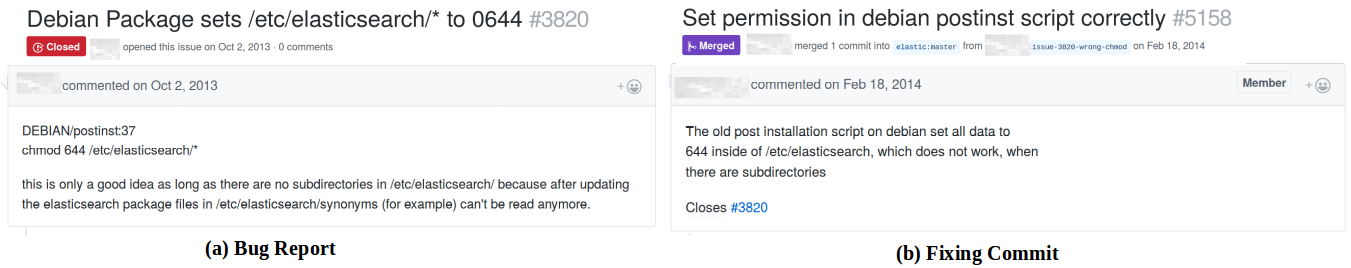
\includegraphics[width=\columnwidth,height=150pt]{img/subdirectories.png}
\caption{Bug caused after changing the version of the software.}
\label{fig:subdirectories}       % Give a unique label
\end{figure}

\begin{figure}[ht]
\centering
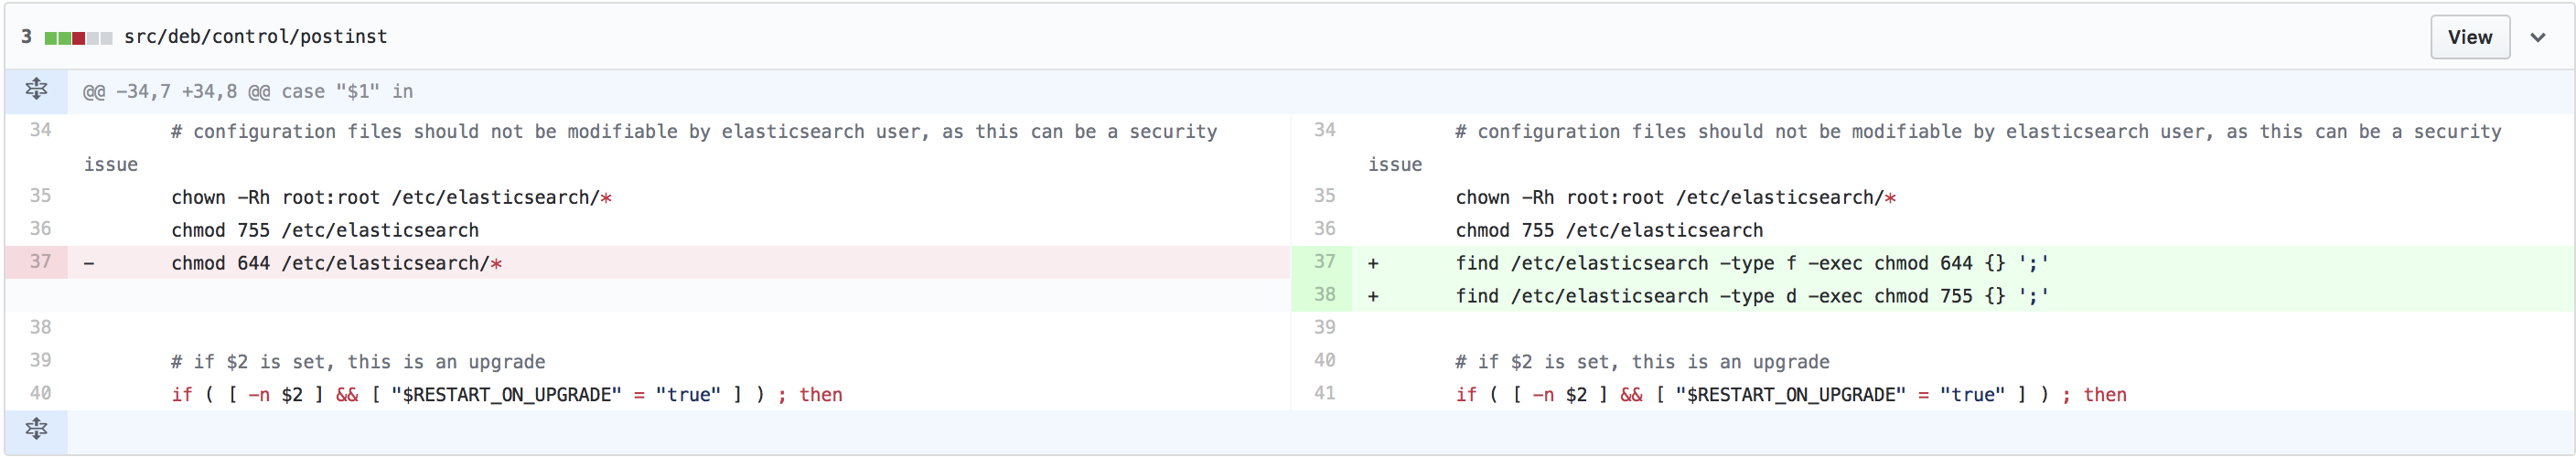
\includegraphics[width=\columnwidth,height=150pt]{img/subdirectoriesfix.png}
\caption{diff of the Bug-Fixing Commit}
\label{fig:subdirectoriesfix}       % Give a unique label
\end{figure}


%Ejemplo de las APIs
The second example is bug \#3551\footnote{https://github.com/elastic/elasticsearch/issues/3551} which is also from ElasticSearch. On the left of Figure~\ref{fig:java} the bug report description is shown and on the right there is the message description of its Bug-Fixing Commit. Below, Figure~\ref{fig:javafix} shows the code in the Bug-Fixing Commit \emph{8668479b9}\footnote{https://github.com/elastic/elasticsearch/commit/8668479b9}. The bug report describes a bug when downloading a site plugin from GitHub. In this case, the dependency of the source code of ElasticSearch on a third-party as GitHub it is what caused the bug. At some point the API of GitHub changed and, as a consequence, the plugin to download \emph{URL} from master zip file does not work, as a result the Bug-Fixing Commit will have to pass the path of GitHub in order to fix the bug. In Figure~\ref{fig:javafix}, it can be observed that to fix the bug, the developer modified two lines \emph{182 and 196}. These modifications however do not mean that the lines were inserting a bug at the moment of the change, but  these lines manifested the failure due to other factors (i.e., a change in a third-party). Thus, as in the above example, none of the previous commits were inserting the bug, so it can be only identified after the change when the bug starts to manifest, meaning it is only possible to identify the First-Failing Commit.
%and the description of its Bug-Fixing Commit \#18140
\begin{figure}[ht]
\centering
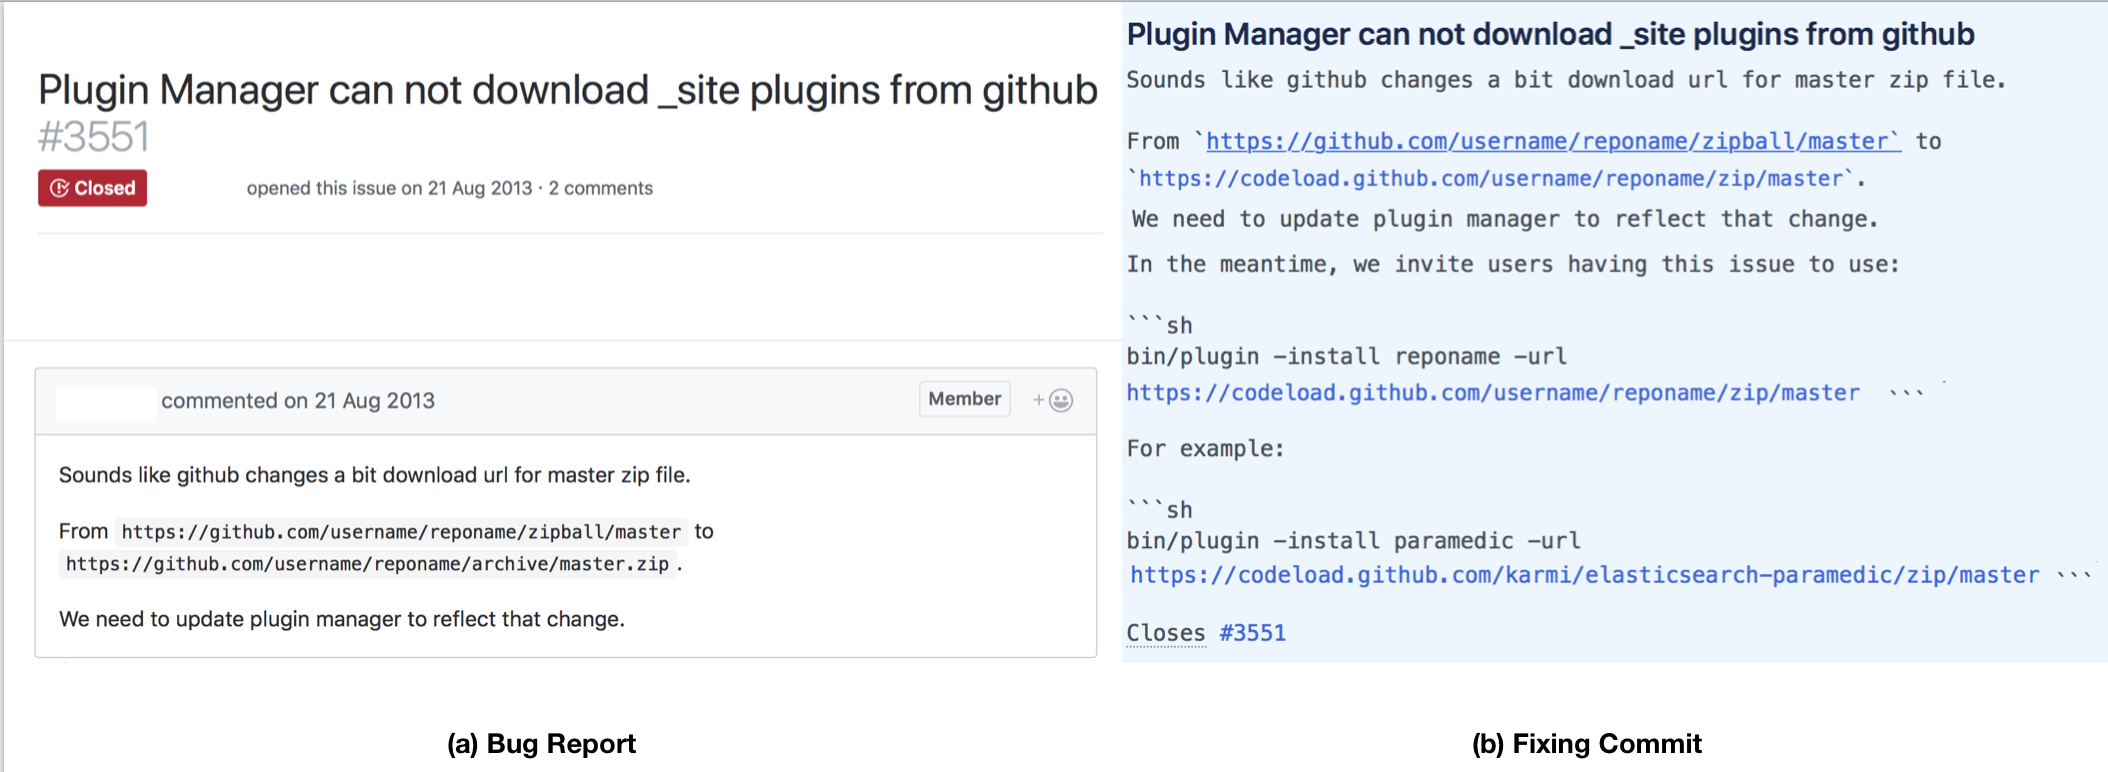
\includegraphics[width=\columnwidth]{img/github.png}
\caption{Bug caused by an external artifact.}
\label{fig:java}       % Give a unique label
\end{figure}

\begin{figure}[ht]
\centering
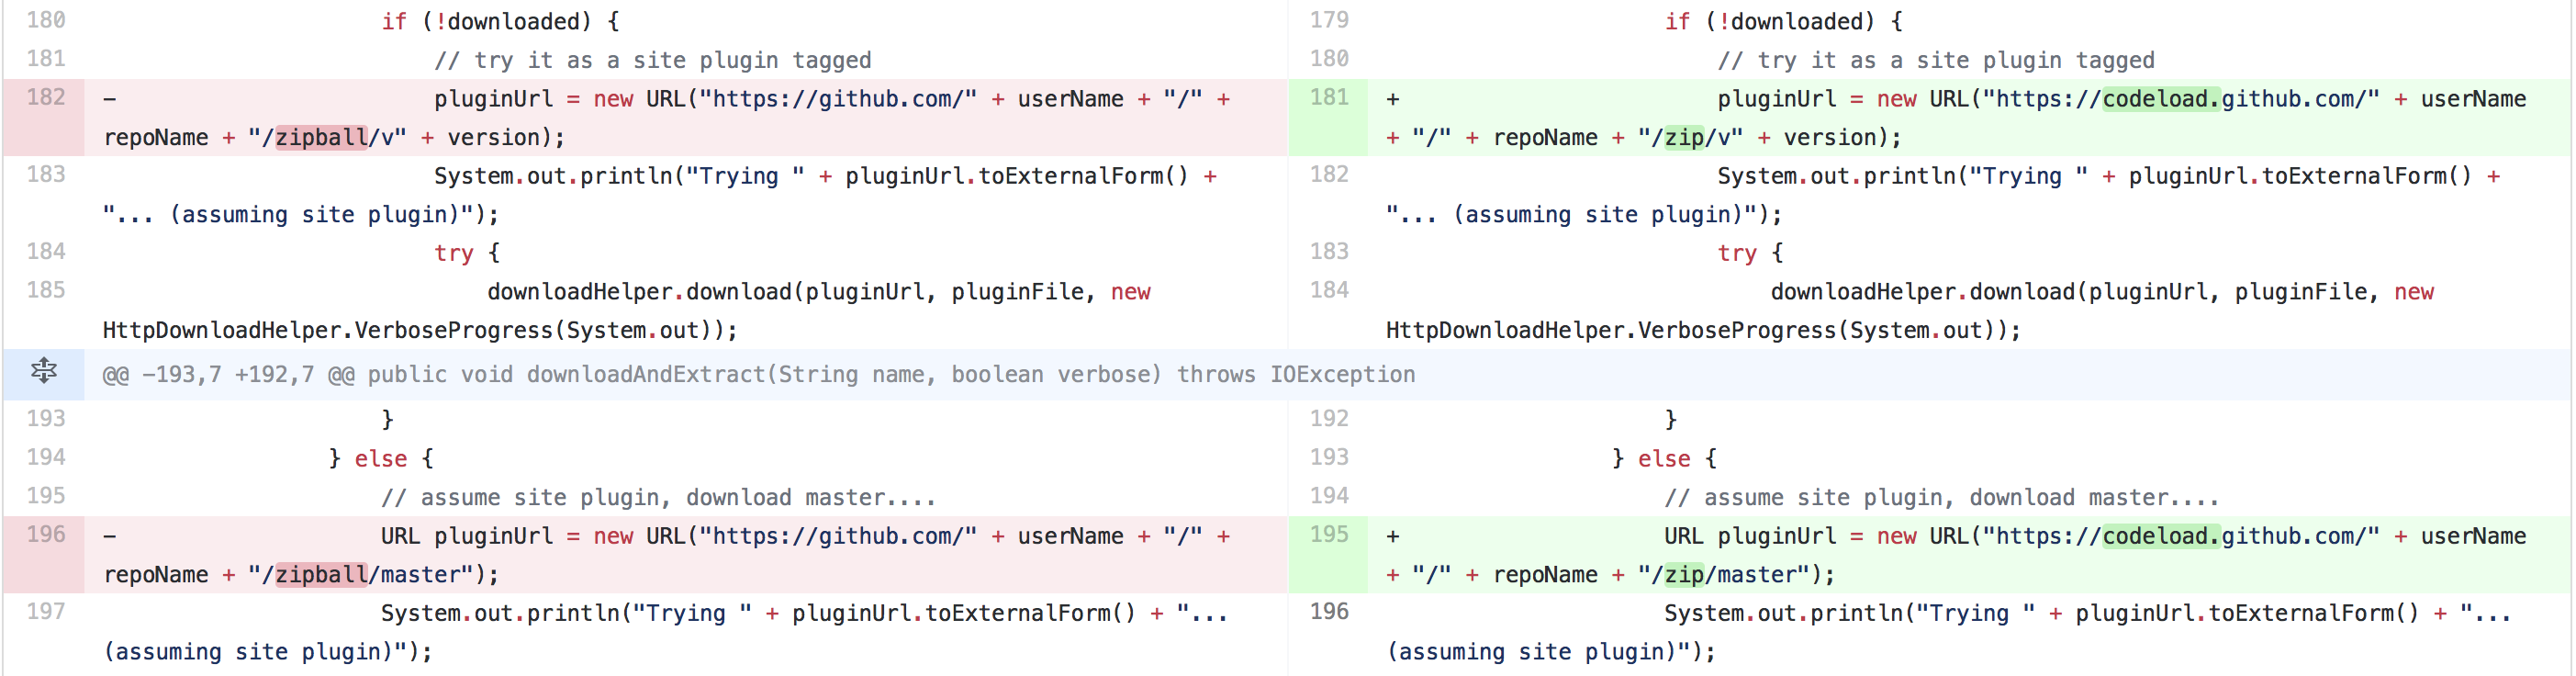
\includegraphics[width=\columnwidth,height=180pt]{img/githubfix.png}
\caption{diff of the Bug-Fixing Commit.}
\label{fig:javafix}       % Give a unique label
\end{figure}

%Ejemplo de windows
Finally, the last example is the bug \#1305897\footnote{https://bugs.launchpad.net/nova/+bug/1305897} from Nova. Figure~\ref{fig:windowsissue} shows the description of the bug report in Launchpad. According to it, the bug was caused by an incompatibility between the software and hardware used. The bug appeared when an option is enabled by default in the VMs;  this option depends on the underlying hardware. Thus, when a user has Windows Server 2012, this option is enabled and it causes the Hyper-V driver to be not aware of the constraint, therefore it becomes not possible to boot new VMs. Figure~\ref{fig:windowsissuefix} shows the Bug-Fixing Commit that modified line \emph{92} and inserted two new lines into the source code. The modification added a new argument into a function. This argument is used in the added lines to check the constrain that caused the bug. Thus, the change that introduced the modified line in the Bug-Fixing Commit cannot be labeled as the Bug-Introduction-Commit. This is because the bug manifests depending on the environment. In this example, the current approaches also identify a false positive Bug-Introduction Commit, because it was correct in the moment of their insertion, while assuming that the developers were not aware of this issue and their intentions were not to make the software compatible in all the possible scenarios.
\begin{figure}[ht]
\centering
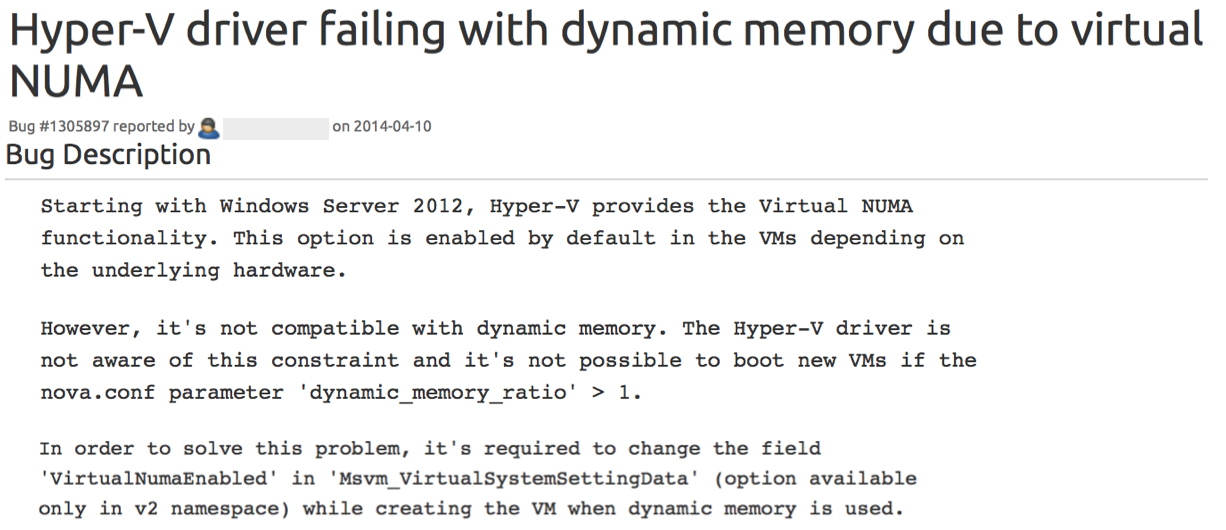
\includegraphics[width=\columnwidth]{img/windowsIssue.png}
\caption{Bug caused by the operating system where the code is being used.}
\label{fig:windowsissue}       % Give a unique label
\end{figure}

\begin{figure}[ht]
\centering
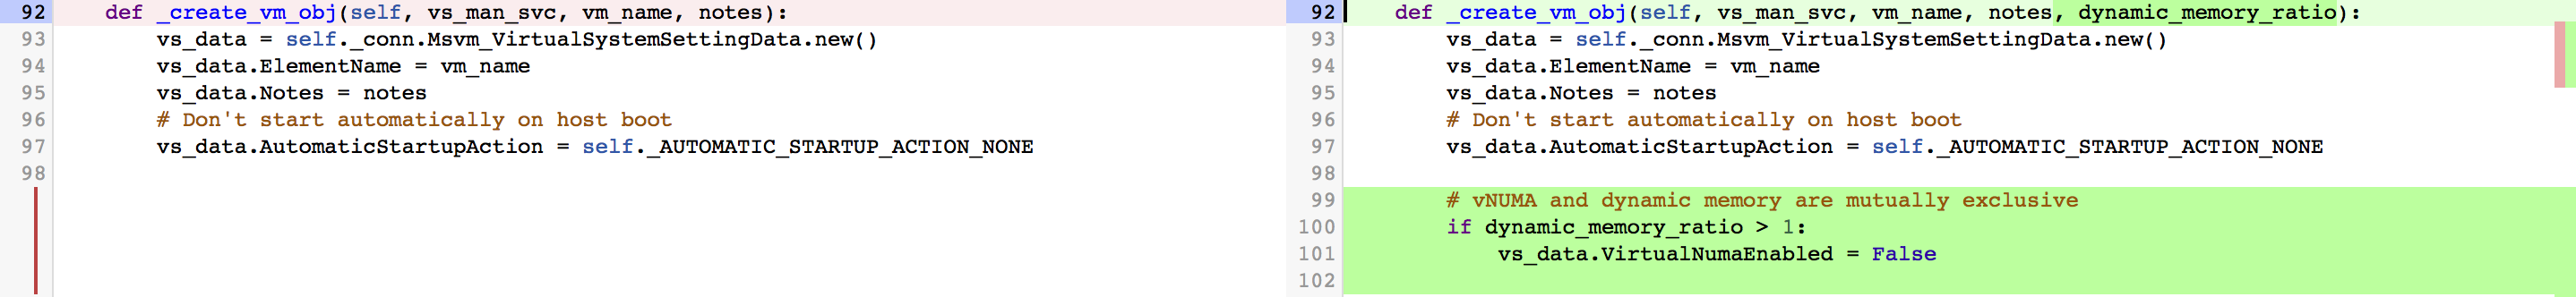
\includegraphics[width=500pt,height=139pt]{img/windowsIssuefix.png}
\caption{Bug caused by an operating system where the code is being used.}
\label{fig:windowsissuefix}       % Give a unique label
\end{figure}

From the demonstration of the real real examples from ElasticSearch and Nova, it is clear that there are cases where  the effect of the external changes, the new requirements and incompatibilities are what caused the failure. These bugs self-manifest without the necessity of having any previous or ancestral changes to introduce the bug into the source code. Hence, in order to find the origin of a bug, not only the fixed lines in the Bug-Fixing Commit  have to be taken into account, the dependencies or ecosystem of such lines must also be considered. It is important to also note that there is no sense to lie a blame on a change as the cause of the bug, because they did not inserted them. However, only the fist change that manifest the bug may be defined within the context of a concrete test system that contains all the dependencies.

\section{The Role of Version Control Systems in the Identification of BIC}
\label{sec:VCS}

This thesis has considerable interest in version control systems \emph{VCS}, since it provides researchers with all the necessary data to analyze and understand the moment when a bug is introduced by first time. It is also the moment when a bug manifests in the project by first time. Thus, it is important to understand how they work and how developers and practitioners have been used them over the last decades. Furthermore, there is special interest for these systems because the selected projects to be analyzed in this thesis use a VCS. It is also because the vast majority of approaches for finding the Bug-Introducing Commit and for predict future bugs use them. 

VCS were developed to coordinate the shared access between many developers to the documents and files. These systems allow for simultaneous development of many branches and can detect any change committed in the source code. Then, these changes are saved along with the information of the timestamp and the identifier of the developer that make them. The VCS of a project keeps track of every modification to the source code and allow developers to turn back to any previous moment and compare earlier versions of the code. They can also revert to the last modification or return to a specific version of the project.

The most common use of these systems is to develop software, but they are also used in content management systems. The best-known VCS are Apache \emph{Subversion (SVN)} and \emph{Git}. The web-based hosting service for Git is GitHub\footnote{https://github.com/}, whereas RiouxSVN\footnote{https://riouxsvn.com/} hosts SVN. Although, Mercurial\footnote{https://www.mercurial-scm.org}, Bazaar\footnote{http://bazaar.canonical.com/en/} and CVS\footnote{https://www.nongnu.org/cvs/} are also well known. These VCS can be classified into two classes; \emph{Centralized VCS} that keep the history of changes on a central server where everyone requests the latest version and pushes the latest changes to.  \emph{Distributed VCS} in when everyone has a local copy of the entire repository. Thus, it is not necessary to push changes to the work all time, it allows for anyone to sync with any other team member.

SVN is a centralized VCS with a unique central repository which hosts all the data for the users. This disables two users from being unable to edit a file at the same time, and that every single change has to be pushed forward immediately.  Figure~\ref{fig:subversion} shows how a SVN project works, in the picture there are three developers with access to modify the files; when Developer \emph{A} modifies a file she has to push the changes to the central repository. Developer \emph{B} and \emph{C} only have the new state of the project after pulling the central repository, furthermore they cannot make any changes to the same file as Developer \emph{A}. While Developer \emph{A} is making changes to a file, other developers are unable to make any modification until Developer \emph{A} finishes and pushes the changes. 

\begin{figure}[ht]
\centering
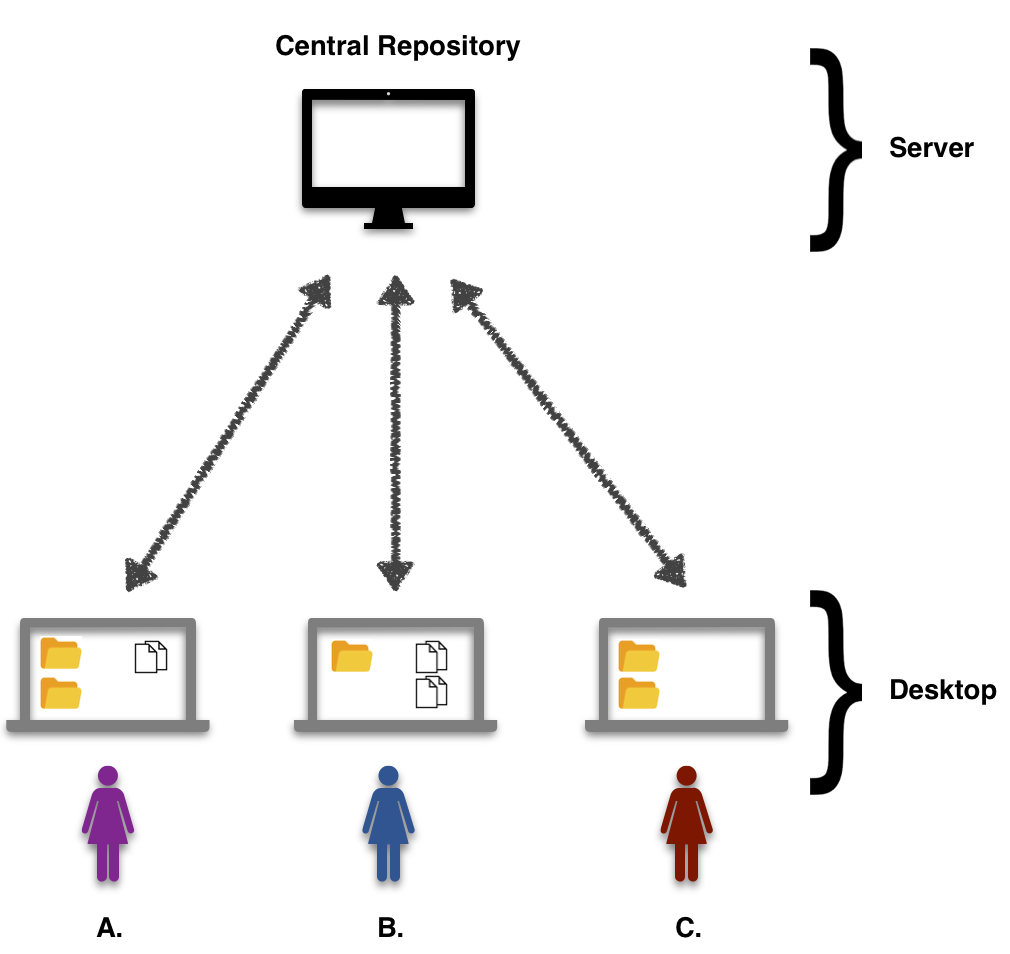
\includegraphics[height= 6cm]{img/subversion.png}
\caption{subversion}
\label{fig:subversion}       % Give a unique label
\end{figure}

On the contrary, Git is a decentralized VCS, it has a unique central repository but each developer has their own local repository. Thus, developers can push their code to their private repository, while getting all the benefit of VCS. They can make their code better after some changes, before pushing the changes from their repository to the central repository and letting other people use their new code. Figure~\ref{fig:git-mercurial} presents how a Git project works, in the picture there are three developers with access to modify the files, each developer has a local copy of the central repository in their computer. Thus, Developer \emph{A}, \emph{B} and \emph{C} can modify the files as many times as they want before pushing the changes to the central repository. This may cause the developers to be in different states of the same project in their local repository because they have not pushed or pulled frequently. In Git, same files can be modified at the same time, however if the developers have changed the same line, the system enters into a conflict that has to be solved before developers can continue committing changes.

\begin{figure}[ht]
\centering
\includegraphics[height= 6cm]{img/git-mercurial.png}
\caption{git-mercurial}
\label{fig:git-mercurial}       % Give a unique label
\end{figure}


Unfortunately, the current approaches used to identify the Bug-Introduction Commits are not understood for the \emph{real} moment of inserting a buggy line in the source code, the cause of the bug, and it force practitioners to apply these approaches to all the projects without regarding the nature of the bug, the dependencies of the bug or even whether they use SVN or Git. It is important to understand why the VCS are relevant when using the approaches to find the \BIC, specifically, because some of the approaches were developed to be used in SVN and they understand the branches in a different way than Git. For example, a branch in Git is only a pointer to some commit which can move and it causes the complete loss of the previous states where this is impossible in SVN. In other words, git does not keep a relationship of the changes setting in time, thus the approaches that use temporally windows to remove false positives or have faith that the precedence between commits is set by dates are not suitable in Git. Furthermore, another characteristic of Git is also the wide variety of commands at our disposal such as \emph{git diff, git remote, git bisect or git blame}. However, some of these options such as \emph{git merge, git rebase or git squash} can alter the natural order of the commits, in the sense that when the history of the commits are viewed using \emph{git log}, it may occur that the commits are not sorted by dates as presumed from the beginning. Hence, the use of Git also can affect the correct identification of Bug-Introducing Commits, and since the project analyzed in this thesis use Git as VCS, how these command affect the identification of the origin of a bug is described in detail. %This happens because of some commands such as \emph{git merge, git rebase or git squash} that might alter the natural order of the commits
%Moreover, as we have explained before, it is not fair to blame changes as the \BIC when in fact they are not the real cause of the bug, so to be more accurate in the results and can learn from the history of the projects taking into account all the factors around, we have proposed to find the \FFC instead of the BIC and, furthermore we must understand that this \FFC has dependencies which help to comprehend the origin of the bug

%The projects that we have studied use Git as control version system. One of the characteristics of Git is also the wide variety of commands at our disposal such as git diff, git remote, git bisect or git blame. However, some options can alter the normal order of the commits, in the sense that when you look at the history of the commits using \emph{git log}, it may happen that the commits are not sorted by dates as we would think in the beginning. This happens because of some commands such as \emph{git merge, git rebase or git squash} that might alter the natural order of the commits.

To better understand how Git might affect the identification of \BIC, this thesis explains three common scenarios with different commands available in Git. All of the scenarios use the same simple example. In the example, the repository only has two diverging branches, the master branch and the feature branch. The commit hashes\footnote{a unique 40 character string generated by the SHA-1 algorithm which takes some data as input and generates the hash} are represented with integers, and in addition, these integers also represent timestamps, where a smaller number means an earlier commit.

\paragraph{Git Merge:} The first scenario is when a developer uses Git Merge. This command is used to create a new commit. This new commit has two different parents and it is the only commit with this characteristic. The only time that Git Merge does not create a new commit is when the developer use the \emph{fast-forward merge} command. This situation occurs when there are no commits in another branch. Figure~\ref{fig:gitmerge} shows the repository before and after the merge. In this case, to see the precedence between commits, \emph{git log} can be typed after merging the branch and the result is a lineal log sorted by date: 7,6,5,4,3,2,1.

\begin{figure}[ht]
\centering
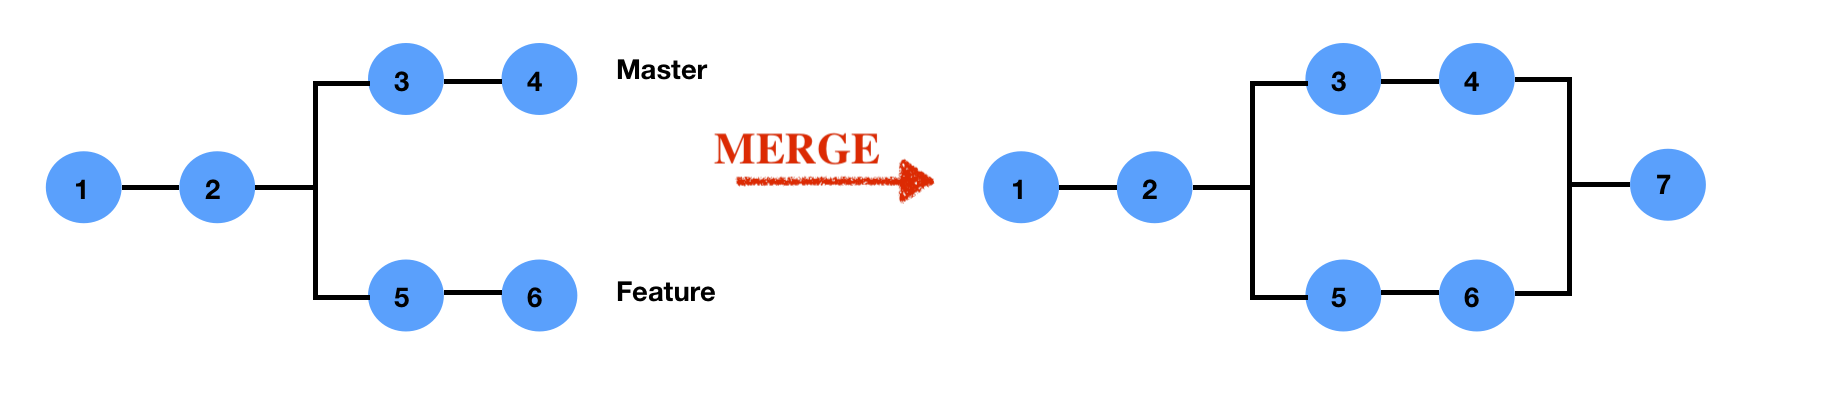
\includegraphics[width=\columnwidth]{img/gitmerge.png}
\caption{git-merge}
\label{fig:gitmerge}       % Give a unique label
\end{figure}

\paragraph{Git Rebase:} The second scenario is when a developer uses Git Rebase. This command recreates the work made from one branch onto another. For example, if a developer wants to rebase the master branch in the feature branch, for every commit that the master branch has that is not in feature branch, a new commit will be created on top of the feature branch. The Figure~\ref{fig:gitrebase} shows the output before and after the rebase from master branch onto feature. In this case, git rebase has moved changes 3 and 4 to the master branch, and it has changed the hash in order to add a new one. In this case, to see the precedence between commits, \emph{git log} can be typed after rebasing, the result is a lineal log that is not sorted by date: 8, 7, 6, 5, 2, 1.
\begin{figure}[ht]
\centering
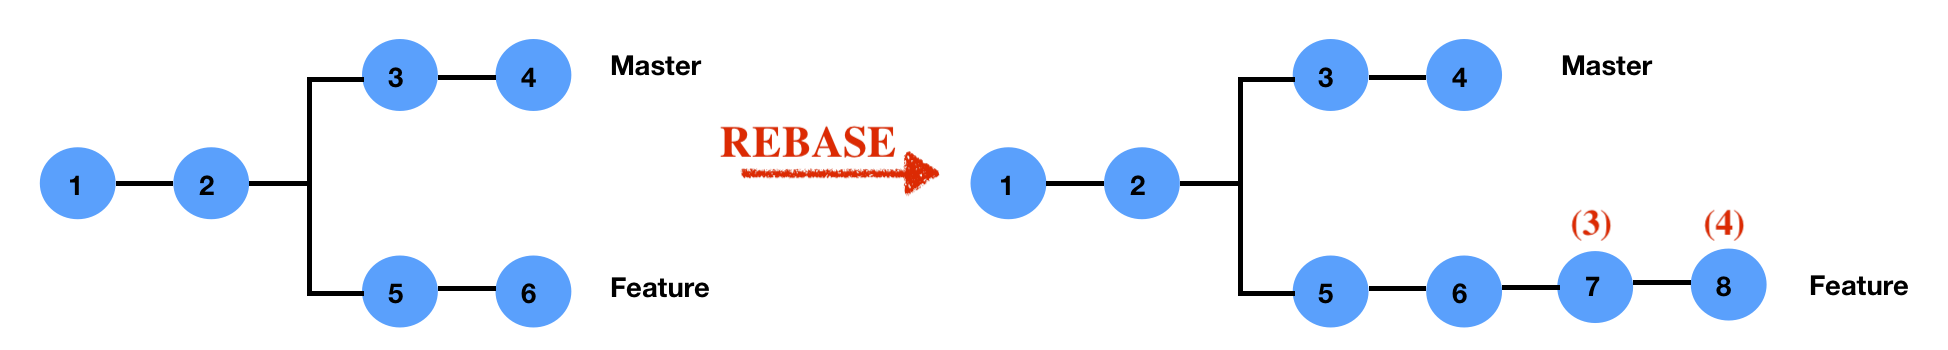
\includegraphics[width=\columnwidth]{img/gitrebase.png}
\caption{git-rebase}
\label{fig:gitrebase}       % Give a unique label
\end{figure}

\paragraph{Git Squash}  The third scenario is when a developer uses Git Squash. This command takes a series of commits and squash them down into a single commit. The main problem of this option is that the authorship of each commit squashed is lost, because these commits disappear from the history. Figure~\ref{fig:gitsquash} shows the output before and after squashing commits 5 and 6 from feature branch onto master. In this case, Git Squash has combined changes 5 and 6 to create a new commit 7,  this commit is then merged with the master branch. In this case, to see the precedence between commits we can type \emph{git log} after squashing, the result is a lineal log  that is sorted by date:  7, 4, 3, 2, 1.
\begin{figure}[ht]
\centering
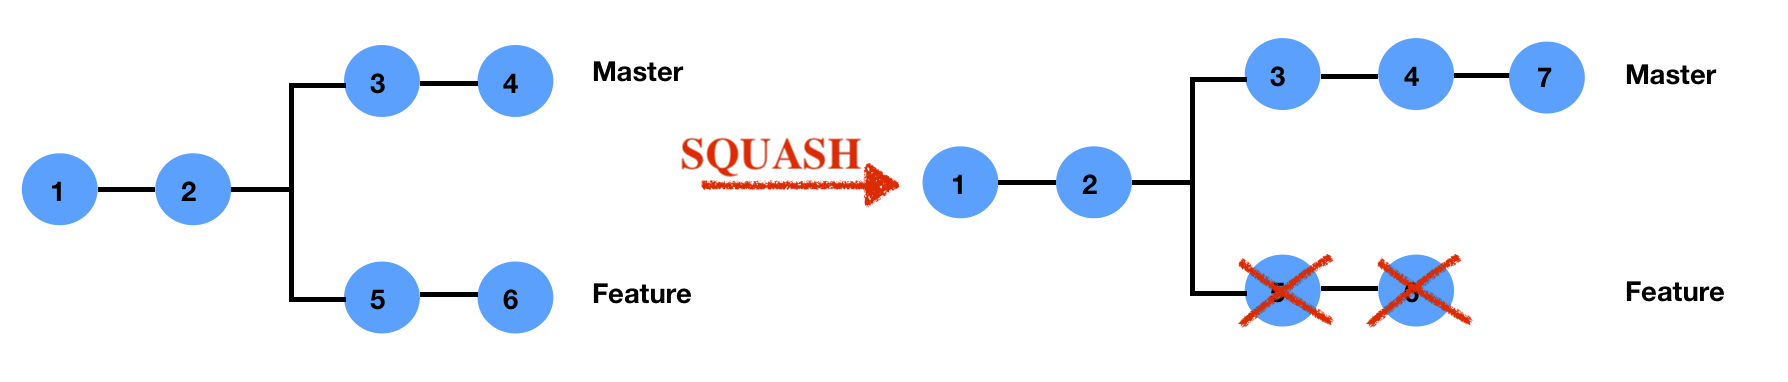
\includegraphics[width=\columnwidth]{img/gitsquash.png}
\caption{git-squash}
\label{fig:gitsquash}       % Give a unique label
\end{figure}

At the end, these types of tool facilitate the interaction between developers when a large number of them work in the same project. They are even more useful when the developers are distributed around the world working in different time zones. However, in order to find the Bug-Introduction Commit, it must be kept in mind that some available options in Git might hint the \emph{real} moment of bug introduction because some commands such as \emph{git merge, git rebase or git squash} that might alter the natural order of the commits and its origin. %Moreover, as we have explained before, it is not accurate to blame changes as the \BIC when in fact they are not the cause of the bug, to be more accurate in the results and can learn from the history of the projects taking into account all the factors around, we have proposed to find the \FFC instead of the BIC and, furthermore we must understand that this \FFC has dependencies which help to comprehend the origin of the bug


%%%%%%%%%%%%%%%%%%%%%%%%%%%%%%%%%%%%%%%%%%%%%%%%%%%%%%%%%%%%%%%%%%%%%%%%%%%%%%%%
%%%%%%%%%%%%%%%%%%%%%%%%%%%%%%%%%%%%%%%%%%%%%%%%%%%%%%%%%%%%%%%%%%%%%%%%%%%%%%%%
% CREDIBILITY IN THE SZZ %
%%%%%%%%%%%%%%%%%%%%%%%%%%%%%%%%%%%%%%%%%%%%%%%%%%%%%%%%%%%%%%%%%%%%%%%%%%%%%%%%

\cleardoublepage
\chapter{Reproducibility and Credibility of the SZZ}
\label{chap:credibility}

Reproducibility of Empirical Software Engineering (ESE) studies is an essential part for improving their credibility, as it offers the opportunity for the research community to verify, evaluate and improve their research outcomes where concerns related to the reliability of the results may arise. Furthermore, it is one of the fundamental characteristics of the scientific method~\cite{gonzalez2012reproducibility}. Juristo and Vegas state that reproducibility ``is important to increase and consolidate the body of empirical knowledge''~\cite{juristo2009using}, and Robles shows that reproducibility may be hindered by many factors~\cite{robles2010replicating}. 

Through this thesis, we adopt the definition of reproducibility by Madeyski and Kitchenham~\cite{madeyski2017would} which claims that ``reproducible research is the extent to which the report of a specific scientific  study can be reproduced (in  effect, compiled) from a reported text, data and analysis procedures, and thus can be validated by other researchers''. Although there are differences between reproducibility and replication, we assume that a research work is more likely to be replicated when it incorporates means of reproducibility. However, reproducibility  (and by extension credibility, since multiple replications of an experiment increase it~\cite{juristo2009using}) may be a challenging work, as access to data sources, use of specific tools, availability of detailed documentation has to be handled. Thus, detecting elements that my hinder reproducibility should help strengthen the credibility of the empirical studies~\cite{perry2000empirical}. 

This chapter addresses how the scientific practice of the ESE research community affects the reproducibility and credibility of the results of studies that use the SZZ algorithm, published in 2005 by {\'S}liwerski, Zimmermann and Zeller~\cite{sliwerski2005changes}  to detect the origin of a bug. The goal is to give a detailed description of the algorithm and explain its limitations and enhancements; then we detail the Systematic Literature Review \emph{(SLR)} in the credibility and reproducibility of the SZZ. Notice that this section is based on the manuscript ``Reproducibility and credibility in empirical software engineering: A case study based on a Systematic Literature Review of the use of the SZZ algorithm'' published in the \emph{Information and Software Technology} Journal. Regarding further details about this section, please refer to the paper.


\section{Description of the SZZ algorithm.}
\label{sec:SZZalgorithm}
%Description of SZZ
In software engineering research, the SZZ algorithm is a popular algorithm for identifying  Bug-Introducing Commits~\cite{da2016framework}. SZZ relies on historical data from version control systems and bug tracking systems to identify change sets in the source code that introduce bugs. The algorithm addresses two different problems. The first problem is related to the linkage between the VCS and the issue tracking system in order to identify the Bug-Fixing Commit; the second problem is related to the identification of the Bug-Introducing Commit.

In the first part, the algorithm identifies, by means of a set of heuristics, Bug-Fixing Commits through using a technique that matches commits with bug reports labeled as \emph{fixed} in the bug tracking system. Therefore it uses regular expressions to identify bug numbers and keywords in the commit messages that are likely to point out a real bug fixing change. This is possible since many projects have adopted the policy of recording the bug report number in the message of the commit that fixed the bug. Thus, the algorithm splits every log message into a stream of tokens to find the potential \emph{bug number} with the use of regular expressions. For instance, the algorithm looks for keywords such as \emph{fix(e[ed]), bugs, defects, patch} followed by a number.

The second part of the algorithm is concerned with the identification of the Bug-Introducing Commit(s). The algorithm employs the \textit{diff} functionality implemented in source code management systems to determine the lines that have been changed (to fix the bug) between the fix commit version and its previous version. Then, using the \textit{annotate/blame} functionality, SZZ is able to locate who modified or deleted those lines for the last time in previous commit(s), and, whether they were committed before the bug was reported; those change(s) are flagged as suspicious of being the Bug-Introducing Commit(s).

As an example, Figure~\ref{fig:code} shows three different snapshots o at different times  and Figure~\ref{fig:history-log} shows when and who changed the code in each commit. The first change is made by Alice on the 1\textsuperscript{st} of June where \textit{12cf3s}, is the Bug-Introducing Commit; the bug is introduced in line 21 because the condition for the \emph{if} statement is used incorrectly. The bug was then reported on the 2\textsuperscript{nd} of June. After that, Becky made the second change on the 3\textsuperscript{rd} of June, \textit{4asd23f}, which added code to the \emph{foo()} function in lines 24, 25 and 26. Finally, the third change, \textit{21esd33} is made by Cloe on the 5\textsuperscript{th} of June. The change fixed the bug by modifying two lines: the buggy line 21 and the clean line 25. In the Bug-Fixing Commit, the modification of line 25 was purely semantic because the line retains with the same behavior from before its modification, in both cases the variable \emph{bar} is incremented by one.

Figure~\ref{fig:SZZalgorithm} shows how the algorithm works. First, after the report of the bug notification \emph{\#159} in the issue tracking system, the algorithm identifies the Bug-Fixing Commit \textit{21esd33} by looking in the logs for a commit with the commit message containing bug number \emph{\#159}. After that, the second part of the algorithm searches for the Bug-Introducing Commit by using the \emph{diff} tool and \emph{annotate/blame} tool in each of the lines modified in the Bug-Fixing Commit. In this example, lines 21 and 25 have been changed in the Bug-Fixing Commit in order to fix the bug, thus both lines are marked for suspicion of being the ones where the bug was introduced. These lines have been inserted in two different commits, however, as line 25 was introduced in a commit after the bug was reported, the algorithm removed it from the list of suspicious Bug-Introducing Commits. Consequently, only the commit that last modified line 21 can be blamed as the Bug-Introducing Commit. Thus, in this case, the SZZ algorithm correctly points out that \textit{12cf3s} is the bug introducing change.

Unfortunately, the algorithm does not always behave as demonstrated in the above example. In some scenarios, the practitioners can notify some of the shortcomings which may cause the malfunction. These shortcomings, as well as some examples of the malfunction of the SZZ are detailed in the next section.

\begin{figure}
\centering
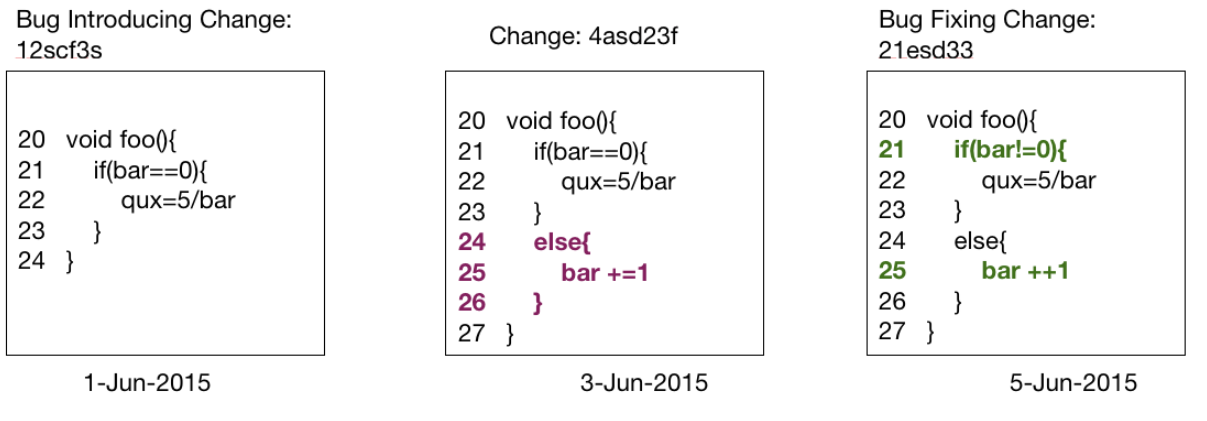
\includegraphics[width=\columnwidth]{img/code.png}
\caption{Example of changes committed in a file, the first change is the bug introducing change and the third change is the bug fixing change. }
\label{fig:code}       % Give a unique label
\end{figure}

\begin{figure}
\centering
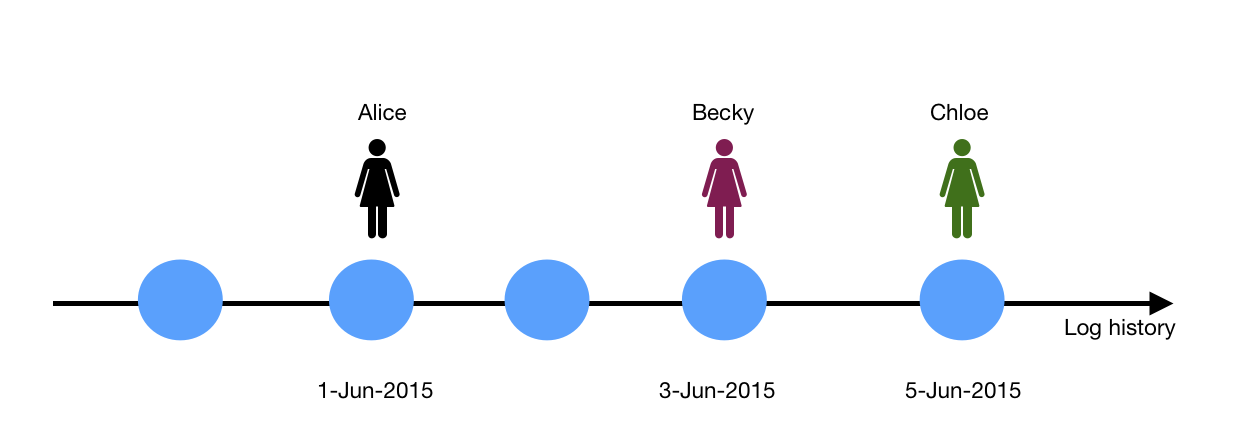
\includegraphics[width=\columnwidth]{img/history-log.png}
\caption{The changes were committed by Alice, Becky and Chloe in different days. }
\label{fig:history-log}       % Give a unique label
\end{figure}

\begin{figure}
\centering
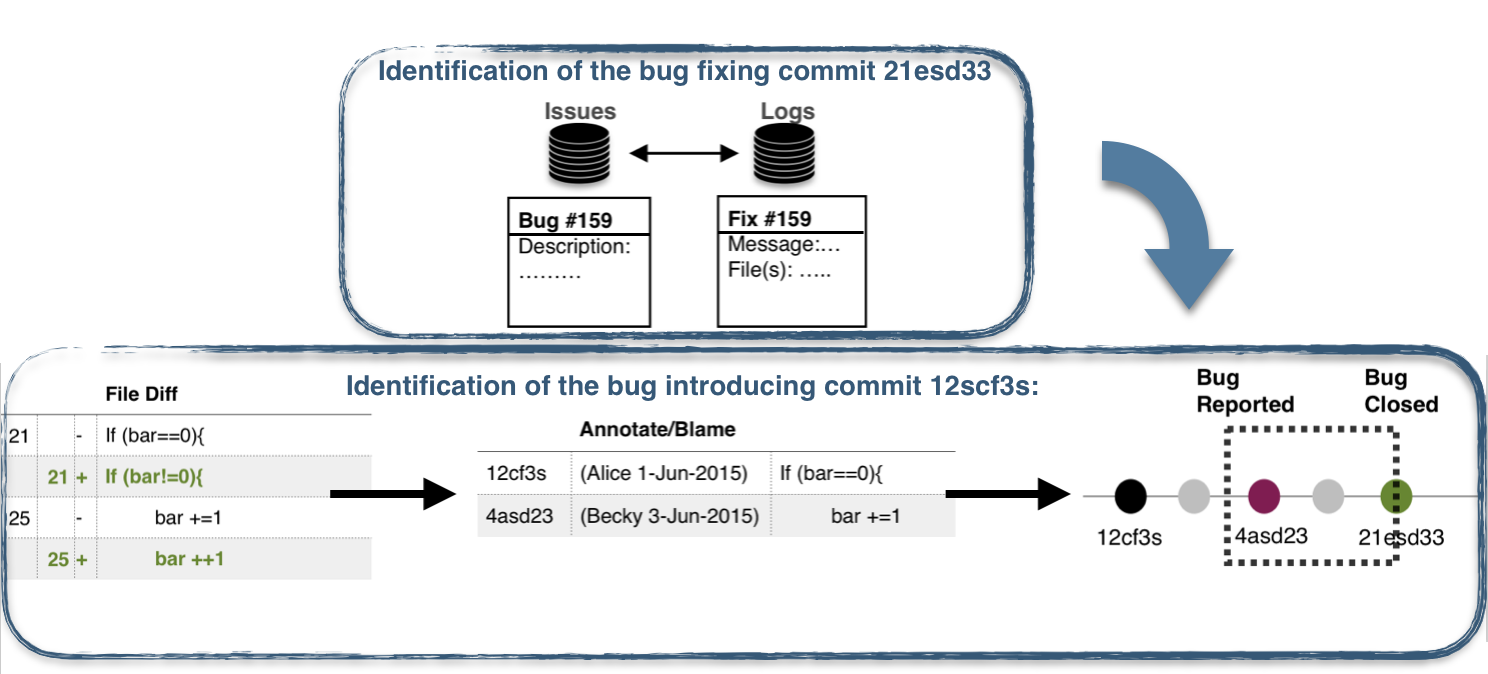
\includegraphics[width=\columnwidth]{img/SZZalgorithm.png}
\caption{First and Second part of the SZZ algorithm}
\label{fig:SZZalgorithm}       % Give a unique label
\end{figure}


\section{Shortcomings of the SZZ Algorithm}
\label{sec:limitations}

Despite SZZ being largely used in ESE to locate bug origins, it presents some shortcomings which makes it error prone. Table~\ref{shortcomingsSZZ} offers a detailed overview of the shortcomings in SZZ as reported in the literature. Some of them have been previously explained in the Chapter \ref{chap:context}, however, in this section they are described with examples based on the illustrative Figure~\ref{fig:code}.

In the first part of the algorithm the limitation lies in how bug reports are linked to commits. If the fixing commit (in the versioning system) does not contain a reference to the bug (usually the reference is the unique id assigned by the bug tracking system, but it could be certain keywords as well), it is very difficult to link both data sources. Sometimes this linking is incorrect as the Bug-Fixing Commit do not correspond to the bug report. If the fixing commit is not identified, the Bug-Introducing Commit cannot be determined and this causes a \emph{false negative}\footnote{The definition of false negative has been addressed in the previous Chapter \ref{chap:context}}. Studies have demonstrated that 33.8\%~\cite{herzig2013s} to 40\%~\cite{rodriguez2016bugtracking} of the bugs in the issue tracker are misclassified, i.e., issues categorized as bugs are actually functionality requests or refactoring suggestions. A false positive\footnote{The definition of false positive has been addressed in the previous Chapter \ref{chap:context}} occurs when a bug report does not describe a real bug, but a fixing commit is still linked to it. Herzig et al. pointed out that 39\% of files marked as defective have never had a bug~\cite{herzig2013s}.

%Furthermore, another issue to take into account is systematic bias: some studies have demonstrated that two out of five issues are misclassified~\cite{herzig2013s},\cite{rodriguez2016bugtracking}. Thus, we have a \emph{false positive} when a bug report does not describe a \emph{real} bug, but a fixing commit is linked to it.

In the second part of the algorithm, lines might be incorrectly identified by SZZ as the place for where the bug was introduced, causing a \emph{false positive}. It may also be that the buggy line was not analyzed by SZZ, producing a \emph{false negative}. In some cases, the bug had been introduced before the last change to the line; then, the history of the line has to be traced back until the \emph{true} source of the bug is found~\cite{williams2008szz}. An example of this can be found when SZZ flags changes to \emph{style} (i.e., non-semantic/syntactic changes such as changes to white spaces, indentation, comments, and some changes that split or merge lines of code) as Bug-Introducing Commits~\cite{da2016framework}, or when a project allows \emph{commit squashing}, since this option removes authorship information resulting in more \emph{false positives}. It may also happen that the bug may have been caused by a change in another part of the system~\cite{german2009change}. A final possibility is that the bug fix modified the surrounding context rather than the problematic lines, thereby misleading the algorithm~\cite{davies2014comparing}.

%\gema{Explain what a false positive, false negative true positive and true negative means here.}
\begin{table}[!t]
% increase table row spacing, adjust to taste
\newcommand{\specialcell}[2][l]{%
  \begin{tabular}[#1]{@{}l@{}}#2\end{tabular}}
\renewcommand{\arraystretch}{0.8}
% if using array.sty, it might be a good idea to tweak the value of
%\extrarowheight as needed to properly center the text within the cells
\caption{Shortcomings that can lead to false negatives when using SZZ.}
\label{shortcomingsSZZ}
\centering
% Some packages, such as MDW tools, offer better commands for making tables
%% than the plain LaTeX2e tabular which is used here.
\begin{adjustbox}{max width=\textwidth}
\begin{tabular}{|l|l|l|}
\hline
Part & Type & Description    \\
\hline
\hline
\multirow{3}*{First part} & Incomplete mapping~\cite{bird2009fair}. & The fixing commit cannot be linked to the bug report. \\  \cline{2-3}
 & Inaccurate mapping~\cite{bissyande2013empirical}.& \specialcell{The fixing commit has been linked to a wrong bug report,\\ they don't correspond each other.} \\ \cline{2-3}
 & Systematic bias~\cite{bird2009fair}.& Linking fixing commits with no \emph{real} bug reports.\\ \hline
\multirow{6}*{Second part} &  Cosmetic changes, comments, etc~\cite{kim2006automatic}.& Variable renaming, indentation, split lines, etc.  \\  \cline{2-3}
 &  Added lines in fixing commits~\cite{da2016framework}.& The new lines cannot be tracked back.  \\  \cline{2-3}
 &  Long fixing commits~\cite{da2016framework}. & The larger the fix the more false positives. \\  \cline{2-3}
 &  Semantic level is weak~\cite{williams2008szz} & Changes with the same behavior are being blamed. \\  \cline{2-3}
 &  Clean changes~\cite{da2016framework}.& \specialcell{This changes start leading to bugs due to external changes \\or artifacts are being blamed.} \\  \cline{2-3}
 & Commit Squashing~\cite{gousios2013ghtorent}.&  \specialcell{This practice might hide the real Bug-Introducing Commit,\\ it combine/merge multiple commits into a single commit loosing authorship information.} \\  \hline
\hline
\end{tabular}
\end{adjustbox}
\end{table}

%\gema{More limitations:Many bug fixes involve touching hundreds or even thousands of lines of code, c.f., many of these lines are changed not because they are root causes but because they need to be modified to facilitate the treatment of the bug. }

\subsection{Some Examples}
\label{subsec:examples}
To provide more insights on the reasons why SZZ identifies false positive commits, we explain three possible scenarios based on the example shown in Figure~\ref{fig:code} in where the algorithm identifies false Bug-Introducing Commits. However, in these scenarios the day of the bug report has changed from the 2\textsuperscript{nd} of June to the 4\textsuperscript{th} of June. Thus, the bug was not reported after the second change was committed, and after applying the heuristics, the SZZ is unable to remove the commit made by Becky from the list of suspicious Bug-Introducing Commits.

The first scenario is represented in the code of Figure~\ref{fig:code} and is related with the problem of identifying more than one Bug-Introducing Commit, and how practitioners should behave. This example shows how after applying the algorithm, it identifies two commits as being the possible Bug-Introducing commits. While the commit made by Alice is correctly identified as a Bug-Introducing commit, the change made by Becky is a false positive because of two main reasons; i) she did not introduce any bug when the lines were committed and, ii) she modified the code but it maintained the same logic of its previous state where line 25 still increments one unit on the variable \emph{``bar''}.

The second scenario is represented in the code of Figure~\ref{fig:code2}. In this scenario, the semantic changes made by Becky are hiding the real Bug-Introduction Commit because she decided to replace the name of the variable \emph{``bar''}  for \emph{``people''}. Even though this change may appear to be inoffensive, it modified the variable name in the buggy line 21 hinting the true Bug-Introducing Commit. Thus, when applying the SZZ algorithm, the outcome is that the last commit which touched buggy line 21 is the commit made by Becky, when in fact, the bug was already in the line when Becky decided to change the name of the variable. In this case, the SZZ identifies a commit but it is not the Bug-Introducing Commit.

Finally, the third scenario is represented in the Figure~\ref{fig:code3}. It shows an example where unchanged lines introduced the bug. In this example, Alice wrote the function \emph{foo()}, but she forgot to add the \emph{if} condition which checks whether the variable \emph{``bar''} is not equal to 0, otherwise the logic in line 22 will fail because it is not allow to divide a variable between 0. Thus, in order to fix the bug Chloe added the \emph{if} condition in the Bug-Fixing Commit. Therefore when the SZZ algorithm is applied, the outcome blames a wrong change as the Bug-Introducing Commit because the bug was fixed by adding a new line, and the SZZ algorithm cannot track back the line.

\begin{figure}
\centering
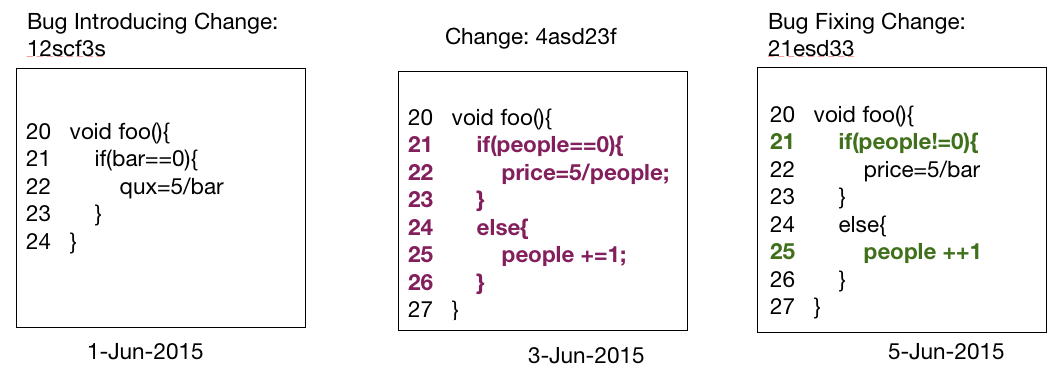
\includegraphics[width=\columnwidth]{img/code2.png}
\caption{Example where semantic changes in the buggy line hide the bug introducing change and the SZZ cannot identify it. }
\label{fig:code2}       % Give a unique label
\end{figure}

\begin{figure}
\centering
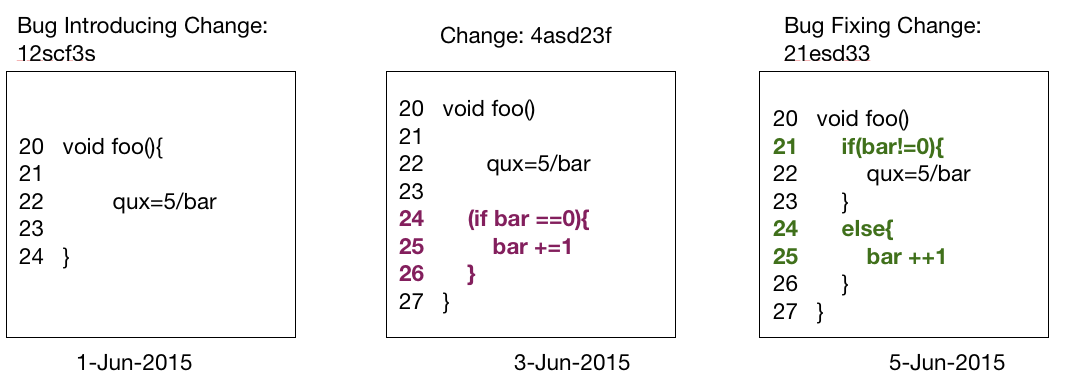
\includegraphics[width=\columnwidth]{img/code3.png}
\caption{Example where unchanged lines introduced the bug, and SZZ cannot identify the Bug-Introducing Commit.}
\label{fig:code3}       % Give a unique label
\end{figure}


\subsection{Enhancements of SZZ}
\label{subsec:Enhancements}
After describing the shortcomings of the SZZ found in the literature, the focus is now on how researchers have addressed them over time and in how far the enhancements have mitigate the problems.

The misclassification problem has been further investigated by researchers, aiming at mitigating the limitations found in the first part of SZZ~\cite{herzig2013s,tan2015online,rodriguez2016bugtracking}. Tools and algorithms have been created based on the information from version control systems and issue tracking systems to map bug reports to fixing commits~\cite{wu2011relink,nguyen2012multi,le2015rclinker,sun2017frlink}. As a result of these efforts, the first part of SZZ has seen how its accuracy has significantly increased. 

Related to the second part of SZZ, two main improvements have been proposed in the literature; they are referred to as SZZ-1 and SZZ-2:
\begin{itemize}
	\item \emph{SZZ-1}) Kim~\textit{et al.} suggest an SZZ implementation that excludes cosmetic changes, and propose the use of an \textit{annotation graph} instead of using \textit{annotate\footnote{Notice that annotate is used in SVN and blame is used in git.}}~\cite{kim2006automatic}.
	\item \emph{SZZ-2}) Williams and Spacco propose to use a mapping algorithm instead of annotation graphs; this approach uses weights to map the evolution of a source code line and ignores comments and formatting changes in the source code with the help of \texttt{DiffJ}, a Java-specific tool~\cite{williams2008szz}.
\end{itemize}

The second part of the algorithm however still has room for further improvements such as the work from Da Costa~\textit{et al.} who have created a framework to eliminate unlikely  Bug-Introducing Commit from the outcome of SZZ. Their framework is based on a set of requirements that consider the dates of the suspicious commit and of the bug report~\cite{da2016framework}. By removing the commits that do not fulfill these requirements, the number of false positives provided by SZZ is lowered significantly.
. As can be seen, addressing the limitations of the SZZ often requires a manual, tedious validation process which can be impractical at times.

\section{Systematic Literature Review on the use of SZZ algorithm}
\label{sec:SLR}

Through this subsection we present the Systematic Literature Review (SLR) on the use of the SZZ algorithm in 187 academic publications in order to address how the scientific practice of the ESE research community affects the reproducibility and credibility of the results. In particular, we want to address studies that use the SZZ algorithm, published in 2005 in ``When do changes induce fixes?'' by {\'S}liwerski, Zimmermann and Zeller~\cite{sliwerski2005changes} at the MSR workshop\footnote{MSR is today a working conference, but at that time it was a co-located workshop with ICSE in its second edition.}.  SZZ has been largely used in academia, counting, as of May 2018, with more than 610 citations in Google Scholar\footnote{https://scholar.google.es/scholar?cites=3875838236578562833}.

The purpose of a SLR is to identify, evaluate and interpret all available studies relevant to a particular topic, research question, or effect of interest~\cite{Kitchenham07guidelinesfor}. A SLR provides major information about the effects of a particular topic across a wide range of previous studies and empirical methods. As a result, a SLR should offer evidence with consistent results and suggest areas for further investigation. To address the SLR, we followed the approach proposed by Kitchenham and Charters~\cite{Kitchenham07guidelinesfor} in order to analyze the credibility and reproducibility of the SZZ algorithm. Therefore, we address the following  questions:
\begin{enumerate}
	\item \textbf{What is the impact of the SZZ algorithm in academia?} The SZZ algorithm has been shown to be a key factor in locating when a change introduced fixing commits. However, many papers use only the first part of the algorithm to link bug fix reports to commits. As the second part of SZZ is shown to encompass significant threats, we identify only those publications that use both parts, or at least the second part, of the SZZ algorithm. In addition to this, we offer other metrics on the publications, such as the number of authors and the geographic diversity of the institutions they work for, in order to provide insight of how widespread the use of SZZ is.
	Furthermore, one of our goals addresses the maturity and diversity of the publications where SZZ has been used in order to understand its audience. We address the \emph{maturity} of a publication by analyzing whether it has been accepted in a workshop, a conference, a journal, or a top journal. Diversity is given by the number of distinct venues where publications using SZZ can be found.
	\item \textbf{Are studies that use SZZ reproducible?}  Reproducibility is a crucial aspect of a credible study in ESE~\cite{gonzalez2012reproducibility}. Piwowar~\emph{et al.} state that reproducibility improves the impact of research~\cite{piwowar2007sharing}. In addition, when a research work incorporates reproducibility, it is more likely to be replicated. However, there is evidence in the ESE literature that replicable studies are not common~\cite{robles2010replicating}. By providing a replication package (or a detailed description of the analysis and the environment and data used), the authors facilitate others to replicate or to reproduce their experiment, which increases the credibility of their results~\cite{juristo2009using}. In addition, replication packages help in the training of novice researchers~\cite{madeyski2017would}. To provide trustworthy results in ESE research, authors should offer a replication package and/or a detailed description of the research steps, and the environment and data used. This would allow others to reproduce or replicate their studies~\cite{gonzalez2012reproducibility}.
	\item \textbf{Do the publications mention the limitations of SZZ?} It has already been shown that limitations of SZZ are well-known in the research literature but there is still the question of how many papers report any of these. Therefore, this chapter also studies whether authors mention the limitations of SZZ that may affect their findings, be it in the \emph{description of the method}, in the \emph{threats to validity} or in the \emph{discussion}.
	\item \textbf{Are the improvements to SZZ (SZZ-1 and SZZ-2) used?} The improved versions of the original SZZ algorithm address some of its limitations. We analyze whether any of the improvements to the SZZ algorithm can be found in the primary studies included in the SLR. Thus, we search for any mention of their use, be it in the \emph{description of the method} or in the \emph{threats to validity}. Answering this research question enables further understanding on how authors who use SZZ behave given the limitations of SZZ.

\end{enumerate}

\subsection{Inclusion Criteria}
\label{subsec:Inclusion}

After enumerating the questions, we present the inclusion and exclusion criteria for the SLR. In addition, we describe the search strategy used for primary studies, the search sources and the reasons for removing papers from the list.
The inclusion criteria address all published studies written in English that cite either:
\begin{enumerate}
  \item The publication where SZZ was originally described,``When do changes induce fixes?''~\cite{sliwerski2005changes}, or
  \item (at least) one of the two publications with improved versions of the algorithm, ``Automatic Identification of Bug-Introducing Changes''~\cite{kim2006automatic} and ``SZZ Revisited: Verifying When Changes Induce Fixes''~\cite{williams2008szz}.  \end{enumerate}
 
There was no need to further investigate the references to the resulting set of publications (a process known as \emph{snowballing}): if one of these papers contained as well a reference to the papers that fit the inclusion criteria, it is assumed to be already in our sample. 

Before accepting a paper into the SLR, we excluded publications that are duplicates, i.e., a \emph{matured} version (usually a journal publication) of a \emph{less matured} version (conference, workshop, PhD thesis\ldots). In those cases, we only considered the \emph{matured} version. When we found a short and a long version of the same publication, we have chosen the longer version.  However, in those cases where the publication is a PhD thesis and a related (peer-reviewed) publication exists in a workshop, conference or journal, the thesis is discarded in favor of the latter, because conference and journal publications are peer-reviewed whereas a PhD theses are not. Documents that are a \emph{false alarm} (i.e., not a \emph{real}, scientific publication) have also been excluded.

\subsection{Search Strategy used for Primary Studies}
\label{subsec:strategy}

The studies were identified using Google Scholar and Semantic Scholar as of November 8\textsuperscript{th} 2016. We have searched exclusively in Google Scholar and Semantic Scholar because of i) their high accuracy in locating citations, providing more results than other databases (from Table~\ref{tableSearch} it can be seen that they contain three times more citations than other platforms, such as the ACM Digital Library), and ii) because it was observed that they offer a superset of the other databases, i.e., it was checked checked that no publication in the other sources is missing from the list provided by Google Scholar and Semantic Scholar. However, Google Scholar gives many \emph{false alarms}, in the sense that they are not publications but slide sets, notes, etc. Examples of those \emph{false alarms} are ``Strathprints Institutional Repository''\footnote{\url{https://core.ac.uk/download/pdf/9032200.pdf}} or ``Home Research''\footnote{\url{http://ieeexplore.ieee.org/document/1382266/\#full-text-section}}), which was removed manually from our set. Some academic databases which are commonly used for SLRs, such as Scopus, could not be employed to gather citations, because SZZ was published at a time when MSR was a workshop, and thus the original publication~\cite{sliwerski2005changes} is not included in those databases.

\begin{table}[!t]
% increase table row spacing, adjust to taste
\renewcommand{\arraystretch}{0.8}
% if using array.sty, it might be a good idea to tweak the value of
%\extrarowheight as needed to properly center the text within the cells
\caption{Number of citations of the SZZ, SZZ-1 and SZZ-2 publications by research databases.}
\label{tableSearch}
\centering
% Some packages, such as MDW tools, offer better commands for making tables
%% than the plain LaTeX2e tabular which is used here.
\begin{adjustbox}{max width=\textwidth}
\begin{tabular}{|l|c|c|c|c|}
\hline
& Google Scholar & Semantic Scholar & ACM Digital Library & CiteSeerX \\
\hline
\hline
\# SZZ & 493 & 295 & 166 & 26 \\
\hline
\# SZZ-1 & 141 & 100 & 60 & 18 \\
\hline
\# SZZ-2 & 26 & 15 & 8 & 0 \\
\hline
\end{tabular}
\end{adjustbox}
\end{table}

\subsection{Study Selection Criteria and Procedures for Including and Excluding Primary Studies}
\label{subsec:selection}
Table~\ref{tableSelectedPapers} shows that our searches elicited 1,070 citation entries. After applying the inclusion criteria described above, a list of 458 papers was obtained. This process was performed by the first author. The process is objective, as it involves discarding false alarms, duplicates, and papers not written in English. 

Then, the first author analyzed the remaining 458 papers looking for the use of SZZ, SZZ-1 and SZZ-2 in the studies. This resulted in 193 papers being removed because of three main reasons: i) they only cited the algorithm as part of the introduction or related work but never used it, ii) they only cited the algorithm to support a claim during their results or the discussion, and iii) the papers were essays, systematic literature reviews or surveys. This process was discussed in advance by all the authors. The second author partially validated the process by analyzing a random subset comprising 10\% of the papers. The agreement between both authors was measured using Cohen's Kappa coefficient, resulting in a value of 1 (perfect agreement). These papers were removed on the basis that they do not answer our research questions. After this process 273 papers were included in this SLR.

\begin{table}[!t]
% increase table row spacing, adjust to taste
\renewcommand{\arraystretch}{0.8}
% if using array.sty, it might be a good idea to tweak the value of
%\extrarowheight as needed to properly center the text within the cells
\caption{Number of papers that have cited the SZZ, SZZ-1 and SZZ-2 publications by joining the research databases Google Scholar and Semantic Scholar during each stage of the selection process.}
\label{tableSelectedPapers}
\centering
% Some packages, such as MDW tools, offer better commands for making tables
%% than the plain LaTeX2e tabular which is used here.
\begin{adjustbox}{max width=\textwidth}
\begin{tabular}{|l|c|c|c|}
\hline
Selection Process & \#SZZ & \#SZZ-1 & \#SZZ-2 \\
\hline
\hline
Papers extracted from the databases & 788 & 241 & 41  \\
\hline
Sift based on false alarms & 29 removed & 10 removed & 2 removed  \\
\hline
Sift based on not available/English writing & 40 removed & 4 removed & 0 removed  \\
\hline
Sift based on duplicates & 308 removed & 187 removed & 32 removed \\
\hline
Full papers considered for review & 411 & 40 & 7 \\
\hline
Removed after reading & 149 removed & 32 removed & 4 removed \\
\hline
Papers accepted to the review & 262 & 8 & 3 \\
\hline
\end{tabular}
\end{adjustbox}
\end{table}

\subsection{Quality Assessment Criteria}
\label{subsec:quality}

The approach employed to study the quality assessment is based on Kitchenham and Charter's~\cite{Kitchenham07guidelinesfor} concept of quality. 
Thus, the assessment is focused on identifying only papers that report factors related with the credibility and reproducibility of the studies using SZZ.
%\alex{rephrase(This is vague, what does it mean?): enough information to allow an overview across studies.}
%We have applied the criteria to ensure that we analyze those papers that fulfill \alex{rephrase(This is vague and doesn't seem to add anything):a basic set of information}. 
The specific criteria are described in the next phase.
%\gema{I propose: Thus, our assessment is focused on identifying only those papers that report different factors related with the credibility and reproducibility of the studies using the SZZ approach. }

\subsubsection{Phase 1: Establishing that the study uses the complete SZZ algorithm}

In this SLR we only consider studies that use the complete algorithm, or at least its second part. Even though shortcomings have been reported in both parts of the SZZ algorithm (see Section~\ref{sec:SZZalgorithm}), most of the shortcomings present in the first part have been successfully addressed in the last years.%\alex{The following sentences are repetition} The second part of the algorithm still presents the major threats in the reliability of SZZ, and as such we will focus on those papers using it.

To analyze the ease of reproducibility of each study, we looked for (1) a replication package provided by the authors or (2) a detailed description. A detailed description must have: (a) precise dates when the data were retrieved from the projects under analysis, (b) the versions of the software and systems used in the analysis, (c) a detailed description of the methods used in each phase of the study, and (d) enumerate the research tools used. It should be noted whether the that we did not inspect whether the replication package is still available, or whether elements in the package make the study reproducible.

It is also important to point out that during this SLR an assumption was made on the availability of the replication package and that it was available at the time when the articles were submitted. And we do not claim the availability of these packages in the long term, because it is possible that some factors such as a change in the author's affiliation, an inaccessible URL or other reasons might cause the package to not be available anymore. For instance, the reproduction package from the original SZZ paper~\cite{sliwerski2005changes} is no longer available.

Applying our criteria to the set of 273 papers, we obtain 187 papers that fulfill this criterion.

\subsection{Extracting Data from Papers}
\label{subsec:extractingdata}

We have read and analyzed the 187 papers, and extracted the following data information to answer the questions:
\begin{enumerate} 
  \item Title, 
  \item Authors,
  \item Countries of the authors' institutions,
  \item Purpose of the study,
  \item Outcome of the study, and
  \item Venue and class of publication (journal, conference, workshop or university thesis). 
\end{enumerate}

%\alex{The next paragraph should be a new section} \gema{I'm not sure if the next paragraph should be a new section....}
Then, in a second phase, we have carefully analyzed each publication looking:
\begin{enumerate} 
  \item For a replication package (as in~\cite{robles2010replicating}).
%  \alex{ How do you assess ease? Did you just check whether a replication package was present? How did you determine whether a description is detailed enough?}
  \item For a detailed description of the methods and data used (as in~\cite{robles2010replicating}).
  \item Whether shortcomings are mentioned.
  \item Whether a manual inspection to verify the results has been done, to answer.
%  \item The type of limitation that has been reported, to answer RQ3.
  \item Whether authors use an improved version of SZZ (differentiating between a version found in the research literature and \emph{ad-hoc} improvements implemented by the authors).
\end{enumerate}

\subsection{Overview across Studies}
\label{subsec:overview}

Cruzes and Dyb\aa\ reported that synthesizing findings across studies is specially difficult, and that some SLRs in software engineering do not offer this synthesis~\cite{cruzes2011research}. For this SLR we have extracted and analyzed both quantitative and qualitative data from the studies, but we have not synthesized the studies, as they are too diverse. Doing a meta-analysis would offer limited and unstructured insight~\cite{clarke2000cochrane} and results would suffer from some of the limitations in SLRs published in other disciplines~\cite{rosenthal2001meta}. Thus, we combined both our quantitative and qualitative data to generate an overview of how authors have addressed the reproducibility and credibility of the studies. The results are presented in Subsection~\ref{subsec:results}. 
In addition, we have constructed a quality measure\footnote{The main goal of this quality measure is to determine the reproducibility and credibility of the studies in the moment in which the study was submitted.} that assesses the ease of reproducibility of a study. This measure is based on the score of five characteristics of the papers that was looked for in the second reviewing phase. If the questions were answered positively, the paper was marked with a positive score, otherwise with a 0:

\begin{enumerate}
 \item Does the study report limitations of using SZZ? (score = 1 point)
 \item Do the authors carry out a manual inspection of their results? (score = 1 point)
 \item Does the study point to a reproducibility package? (score = 2 point)
 \item Does the study provide detailed description of the methods and data used? (score = 1 point)
 \item Does the study use an improved version of SZZ? (score = 2 point)
\end{enumerate}

%\gema{Look at the next paragraph has been changed}\\
We believe that elements with a higher impact on ease reproducibility of the studies should be scored with 2 points. Partial scores are summed up to obtain an overall score. Table~\ref{tableScore} offers a mapping of this overall measure with the ease of reproducibility of a study.
%\alex {Are reprod and credibility the same?if yes, why would you use 2 terms, if not, what is the difference?}\gema{Done!}
\begin{table}[!t]
% increase table row spacing, adjust to taste
\renewcommand{\arraystretch}{0.8}
% if using array.sty, it might be a good idea to tweak the value of
%\extrarowheight as needed to properly center the text within the cells
\caption{Mapping of overall score and the quality measure on ease of reproducibility of a study.}
\label{tableScore}
\centering
% Some packages, such as MDW tools, offer better commands for making tables
%% than the plain LaTeX2e tabular which is used here.
\begin{tabular}{|c|c|}
\hline
Score & Quality Measure \\
\hline
\hline
 0 -- 1 & \emph{Poor} to be reproducible and to have credible results  \\
\hline
 2 -- 4 & \emph{Fair} to be reproducible and to have credible results  \\
\hline
 5 -- 6 & \emph{Good} to be reproducible and to have credible results  \\
\hline
 7 & \emph{Excellent} to be reproducible and to have credible results \\
\hline
\end{tabular}
\end{table}


\subsection{Results of Questions}
\label{subsec:results}

\subsubsection{Data analysis}

%\alex{All these tables all well but should be somehow discussed. What conclusion can one derive form  looking at the data?}\gema{Done, please see the results again in order to find the discussion of the tables.} 

Here, we present our quantitative and qualitative data analysis extracted from the 187 studies analyzed during the SLR. Table~\ref{tablequantitative} summarizes the frequency of the different outcomes, purposes, versioning systems and  metrics in the studies. 
The most common purpose is \emph{bug prediction} followed by \emph{bug proneness}. %\gema{Notice that it is necessary to provide credible results when using SZZ because the most used purpose is bug prediction, and to be accurate predicting bugs we need to be sure which was the bug introduction commit.}
The most common outcomes are the \emph{development of a new method/approach} and the \emph{evidence of empirical results}. %\gema{However, it seems that the researchers does not use the original SZZ, because new methods/approaches represent 41\% of the outcomes}. 

The qualitative data, summarized in Table~\ref{tablequalitative}, consists in the number of papers that belong to each quality measure levels. It can be observed that 67\% of the papers present a fair reproducibility measure, and only 2\% of them provide excellent means to be reproducible. 
%\gema{Thus, these percentages indicate that we still need to work in providing reproducibility.  Most of the studies are fairly reproducibles which means that the results might not be verified, evaluated or improved and this has a negative impact in the reliability of the study.}


\begin{table}[!t]
\newcommand{\specialcell}[2][c]{%
  \begin{tabular}[#1]{@{}c@{}}#2\end{tabular}}
% increase table row spacing, adjust to taste
\renewcommand{\arraystretch}{0.8}
% if using array.sty, it might be a good idea to tweak the value of
%\extrarowheight as needed to properly center the text within the cells
\caption{Quantitative results from the 187 studies.}
\label{tablequantitative}
\centering
\begin{adjustbox}{max width=\textwidth}
 \begin{tabular}{*{4}{|c}|}%%{|c|c|c|c|}
\hline
Purpose: & Outcome: & Common Metrics: & Versioning:  \\
\hline
\hline
\specialcell{Bug Prediction (BP) (32\%)\\Bug Proneness (BProne) (27\%)\\Bug Detection (BD) (22\%)\\Bug Location(BL) (19\%)} & \specialcell{New Method/Approach (NM) (41\%)\\Empirical Study (ES) (37\%)\\New Tool (NT) (8\%)\\Human Factors (HF) (8\%)\\ Replication (R) (3\%)\\Create a Dataset (D) (2\%)} & \specialcell{Commits (26\%)\\Bug Reports (16\%)\\LOC (15\%)\\Changes (12\%)\\Files (8\%)\\Faults (8\%)\\Revisions (6\%)\\Modules (4\%)} & \specialcell{CVS (50\%)\\Git (28\%)\\SVN (25\%)\\Mercurial (6\%)}\\
\hline
\end{tabular}
\end{adjustbox}
\end{table}

 \begin{table}[!t]
\renewcommand{\arraystretch}{0.8}
% if using array.sty, it might be a good idea to tweak the value of
%\extrarowheight as needed to properly center the text within the cells
\caption{Results of the calculating the quality measure of reproducibility and credibility.}
\label{tablequalitative}
\centering
% Some packages, such as MDW tools, offer better commands for making tables
%% than the plain LaTeX2e tabular which is used here.

\begin{tabular}{|l|c|}
\hline
Quality Measure & \#papers \\
\hline
\hline
Poor to be reproducible and to have credible results &  34 (18\%)\\
\hline
Fair to be reproducible and to have credible results & 126 (67\%)\\
\hline
Good to be reproducible and to have credible results & 24 (13\%)\\
\hline
Excellent to be reproducible and to have credible results & 3 (2\%)\\
\hline
\end{tabular}
\end{table}

The combination of quantitative and qualitative data is addressed in Table~\ref{tablequalitative&quantitative}, where the purpose and outcome of each individual study is grouped according to our quality measure.
It can be observed that the distribution by purpose or outcome does not differ much from the global distribution, although studies offering new tools (NT) and replications (R) offer slightly better results than the rest.

\begin{table}[h!]
\caption{Distribution of the ease of reproducibility quality measure of studies depending on purpose and outcome. Acronyms are defined in Table~\ref{tablequantitative}.}
\label{tablequalitative&quantitative}
  \centering
  \begin{adjustbox}{max width=\textwidth}
  \begin{tabular}{|c|c|c|c|c||c|c|c|c|c|c|c|c|c|}
  \hline
\multicolumn{1}{|c|}{\bfseries Quality} & \multicolumn{4}{|c||}{\bfseries Purpose} & \multicolumn{6}{|c|}{\bfseries Outcome} \\
&\multicolumn{1}{|c|}{\bfseries BP}&\multicolumn{1}{|c|}{\bfseries BProne}&\multicolumn{1}{|c|}{\bfseries BD}&\multicolumn{1}{|c||}{\bfseries BL}&\multicolumn{1}{|c|}{\bfseries ES}&\multicolumn{1}{|c|}{\bfseries HF}&\multicolumn{1}{|c|}{\bfseries NM}&\multicolumn{1}{|c|}{\bfseries NT}&\multicolumn{1}{|c|}{\bfseries R}&\multicolumn{1}{|c|}{\bfseries D}\\
%& BP & BProne & BD & BL & \multicolumn{6}{|c|}{\bfseries Outcome}\\  &&&&& ES & HF & NM & NT & R & D\\
  \hline
  \hline
  Poor & 15 (25\%)&10 (19\%)&6 (15\%)&3 (9\%)&14 (20\%)&2 (13\%)&17 (22\%)&1 (7\%)&0 (0\%)&0 (0\%)\\
\hline
Fair &38 (64\%)&32 (62\%)&29 (72\%)&27 (77\%)&49 (70\%)&13 (81\%)&50 (65\%)&8 (53\%)&3 (60\%)&3 (75\%)\\
\hline
Good &6 (10\%)&9 (17\%)&5 (13\%)&4 (11\%)&5 (7\%)&1 (10\%)&10 (13\%)&5 (33\%)&2 (40\%)&1 (25\%)\\
\hline
Excellent &1 (1\%)&1 (2\%)&0 (0\%)&1 (3\%)&2 (3\%)&0 (0\%)&0 (0\%)&1 (7\%)&0 (0\%)&0 (0\%)\\
\hline
\end{tabular}
\end{adjustbox}
\end{table}

The type of paper (journal, conference, workshop and university thesis) as well as the size (short, medium, long) of the paper might be a restriction to provide means of reproducibility. 
We have labeled paper size to be less than 8 pages for short, from 9 to 50\footnote{We argue that master and PhD theses should be categorized as long publications. We have chosen 50 as limit between medium and long papers because in our data we have observed that all master theses have more than 50 pages whereas none of the journals articles have more than 50 pages.} pages for medium, and more than 50 pages for long publications. Table~\ref{tableTypeSize} reports the type and the size of each individual study grouped according to our quality measure of reproducibility and credibility.
Again, the results do not differ much from the global distribution. 
However, it can be seen that (a) workshop papers perform worse than the rest, and (b) reproducibility increases slightly with the size of the publication.
 
%most of the papers have a \emph{fair} reproducibility, which means that they might be independent of the type and size of the paper.

\begin{table}[h!]
\caption{Results to measure the ease of reproducibility and credibility of the studies depending on the type of paper and their size.}
\label{tableTypeSize}
  \centering
  \begin{adjustbox}{max width=\textwidth}
  \begin{tabular}{|c|c|c|c|c||c|c|c|c|c|c|}
  \hline
\multicolumn{1}{|c|}{\bfseries Quality} & \multicolumn{4}{|c||}{\bfseries Venue} & \multicolumn{3}{|c|}{\bfseries Size} \\
&\multicolumn{1}{|c|}{\bfseries Journal}&\multicolumn{1}{|c|}{\bfseries Conference}&\multicolumn{1}{|c|}{\bfseries Workshop}&\multicolumn{1}{|c||}{\bfseries University}&\multicolumn{1}{|c|}{\bfseries Short}&\multicolumn{1}{|c|}{\bfseries Medium}&\multicolumn{1}{|c|}{\bfseries Long}\\
%& BP & BProne & BD & BL & \multicolumn{6}{|c|}{\bfseries Outcome}\\  &&&&& ES & HF & NM & NT & R & D\\
  \hline
  \hline
  Poor & 5 (12\%)&20 (20\%)&5 (38\%)&4 (13\%)&10 (26\%) &21 (17\%)&3 (13\%)\\
\hline
Fair &32 (76\%)&65 (63\%)&7 (54\%)&22 (74\%)&25 (64\%) &85 (68\%)&16 (70\%)\\
\hline
Good &4 (10\%)&15 (15\%)&1 (8\%)&4 (13\%)&4 (10\%)&16 (13\%)&4 (17\%)\\
\hline
Excellent &1 (2\%)&2 (2\%)&0 (0\%)&0 (0\%)&0 (0\%)&3 (2\%)&0 (0\%)\\
\hline
\end{tabular}
\end{adjustbox}
\end{table}


\subsubsection{What is the impact of the SZZ algorithm in academia?}

Figure~\ref{fig:evolveSZZ} shows the evolution of the number of publications that have cited and used SZZ, SZZ-1 or SZZ-2 up to November 2016. The SZZ algorithm was published in 2005 and afterwards 178 studies have cited it. SZZ-1 was published in 2006 and its number of citations is 53. Finally, SZZ-2 was published in 2008 and counts with 16 publications\footnote{Note that a paper can cite more than one version of SZZ.}.

The number of studies per year peaked in 2013, with 30 papers using an SZZ version. In general since 2012, the number of studies using this algorithm seems to have stabilized with over 15 citations/year for the use of the complete algorithm.

\begin{figure}
\centering
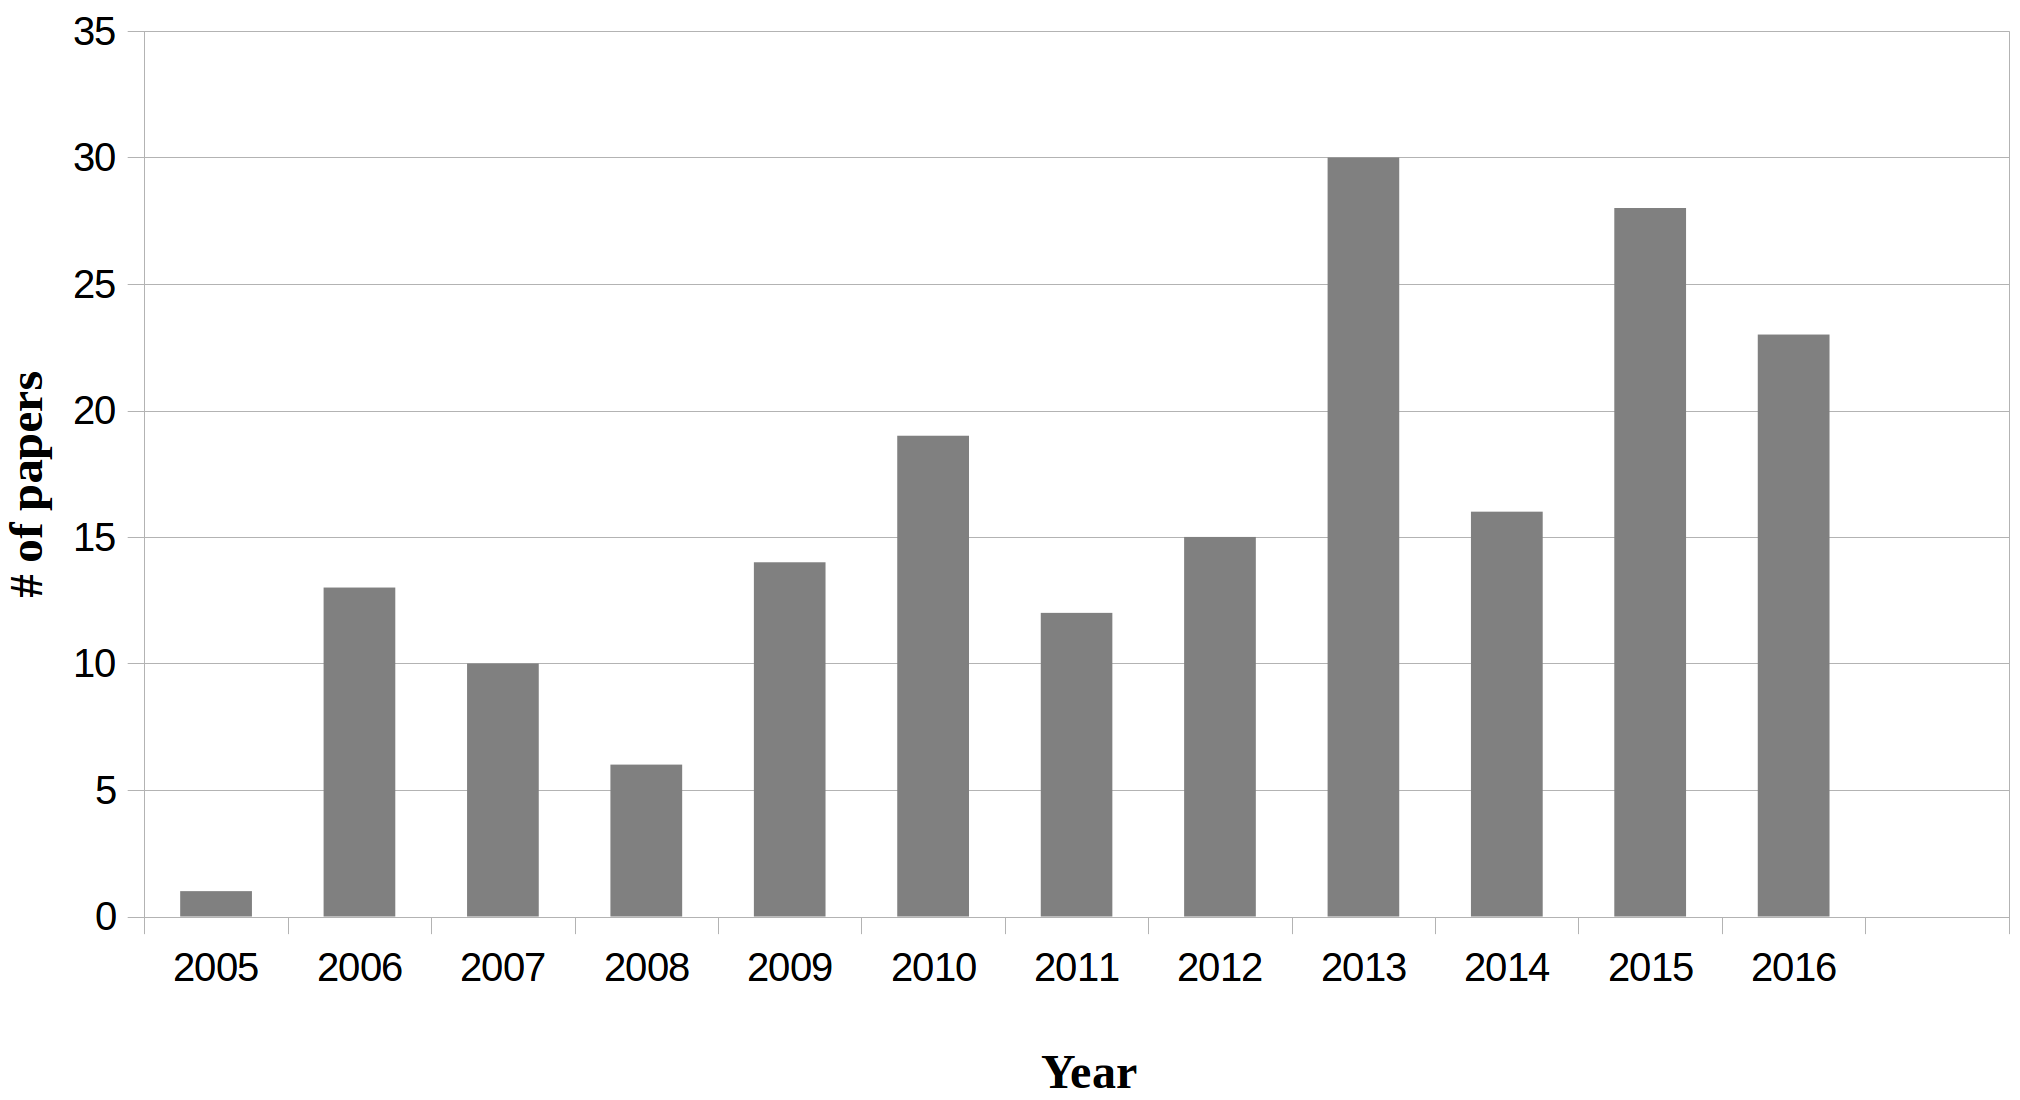
\includegraphics[width=\columnwidth]{img/evolveSZZ.png}
\caption{Sum of the number of publications using the (complete) SZZ, SZZ-1 or SZZ-2 by year of publication (N=187).}
\label{fig:evolveSZZ}       % Give a unique label
\end{figure}

Table~\ref{tableMedia} shows the different types of venues with publications where SZZ has been used. We have classified the venues in four different categories: university theses, workshop papers, conference and symposium publications, and journal articles.
Master theses, student research competitions and technical reports have been grouped under \emph{university theses}.
Diversity and maturity can be found in the sample, as it can be seen from the number of different venues (second column in Table~\ref{tableMedia}) and the considerable number of journal publications (third column in Table~\ref{tableMedia}).

%\alex{Refer to core rankings to justify why you believe MSR, ICSE, ICSME etc to be good conferences. At the same time you can argue.... the impact of SZZ is limited to people conducting empirical studies....... }\gema{Almost done}
\begin{table}
% increase table row spacing, adjust to taste
\renewcommand{\arraystretch}{0.8}
% if using array.sty, it might be a good idea to tweak the value of
%\extrarowheight as needed to properly center the text within the cells
\caption{ Most frequent types of publications using (the complete) SZZ (N=187). \emph{\# different} counts the different venues, \emph{\# publications} counts the total number of publications in that type of venues.}
\label{tableMedia}
\centering
% Some packages, such as MDW tools, offer better commands for making tables
%% than the plain LaTeX2e tabular which is used here.
\begin{adjustbox}{max width=\textwidth}
\begin{tabular}{|l|r|r|}
\hline
Type & \# different & \# publications  \\
\hline
\hline
 Journals & 21 & 42\\
\hline
 Conferences \& Symposiums & 40 & 102\\
\hline
Workshops & 13 & 13\\
\hline
University theses & 20 & 30 \\
\hline
\end{tabular}
\end{adjustbox}
\end{table}

Table~\ref{tableConferences} offers further insight into venues that have published more studies that use SZZ. The most frequent is the conference where SZZ itself was presented, the Working Conference on Mining Software Repositories (MSR). Two top conferences, such as the International Conference on Software Maintenance and Evolution (ICSME) and the International Conference of Software Engineering (ICSE), are second and third. SZZ can also been frequently found in high quality journals, such as Empirical Software Engineering (EmSE) and Transactions on Software Engineering (TSE).
The quality rating of conferences given in Table~\ref{tableConferences} has been obtained from the GII-GRIN-SCIE (GGS) Conference Rating\footnote{http://gii-grin-scie-rating.scie.es/}; Class 1 (CORE A*) conferences are considered \emph{excellent, top notch events} (top 2\% of all events), while Class 2 (CORE A) are \emph{very good events} (given by the next top 5\%). For journals, we offer the quartile as given by the well-known Journal Citation Reports (JCR) by Clarivate Analytics (previously Thomson Reuters).

\begin{table}[!t]
% increase table row spacing, adjust to taste
\renewcommand{\arraystretch}{0.8}
% if using array.sty, it might be a good idea to tweak the value of
%\extrarowheight as needed to properly center the text within the cells
\caption{Most popular media with publications using SZZ, SZZ-1 and SZZ-2 (N=187). ``J'' stands for journal and ``C'' for conference/symposium.}
\label{tableConferences}
\centering
% Some packages, such as MDW tools, offer better commands for making tables
%% than the plain LaTeX2e tabular which is used here.
\begin{adjustbox}{max width=\textwidth}
\begin{tabular}{|c|p{7.6cm}|c|c|}
\hline
Type & Name & Rating & \# papers)  \\
\hline
\hline
C & Conf Mining Softw Repositories (MSR) & Class 2 - CORE A & 15 (8\%) \\
\hline
C & Intl Conf Software Eng (ICSE)& Class 1 - CORE A* & 12 (6\%) \\
\hline
C & Intl Conf Soft Maintenance (ICSME) & Class 2 - CORE A & 10 (5\%) \\
\hline
J& Empirical Software Eng (EmSE) & JCR Q1 & 9 (5\%) \\
\hline
J & Transactions on Software Eng (TSE) & JCR Q1 & 9 (5\%) \\
\hline
C & Intl Symp Emp Soft Eng \& Measurement (ESEM) & Class 2 - CORE A & 8 (4\%)\\
\hline
C & Intl Conf Automated Softw Eng (ASE)& Class 2 - CORE A& 7 (4\%) \\
\hline
C &  Symp Foundations of Software Eng (FSE) & Class 1 - CORE A* & 6 (3\%) \\
\hline
\end{tabular}
\end{adjustbox}
\end{table}

The impact of the SZZ algorithm is significant: 458 publications cite SZZ, SZZ-1 or SZZ-2; 187 of these use the complete algorithm. The popularity and use of SZZ has risen quickly from its publication in 2005 and it can be found in all types of venues (high \emph{diversity}), ranging from top journals to workshops and PhD theses; SZZ related publications have often been published in high quality conferences and top journals (high \emph{maturity}).

\subsubsection{Are studies that use SZZ reproducible?:}
Table~\ref{tableReplication} shows the number of analyzed studies that a) offer a replication package or b) have carefully detailed the methodology and the data used to allow the reproducibility of their studies. We have classified the publications in four groups: i) publications that offer a replication package (\emph{Package}), ii) publications that detail the methodology and data used (\emph{Environment}), iii) publications that have both (\emph{Both}), and iv) none (\emph{None}).

From the 187 analyzed publications, 43 offer a replication package, and 96 carefully detail the steps followed and the data used. Furthermore, only 24 provide both the replication package and the detailed methodology and data. 72 of the papers do not offer a replication package or a detailed description of the methodology and data.

\begin{table}[!t]
% increase table row spacing, adjust to taste
\renewcommand{\arraystretch}{0.8}
% if using array.sty, it might be a good idea to tweak the value of
%\extrarowheight as needed to properly center the text within the cells
\caption{Publications by their reproducibility: Rows: \emph{Yes} means the number of papers that fulfill each column, whereas the complement is \emph{No}. Columns: \emph{Package} is when they offer a replication package, \emph{Environment} when they provide a detailed methodology and dataset. Note that \emph{Both} is the intersection of \emph{Package} and \emph{Environment}. (N=187)}
\label{tableReplication}
\centering
% Some packages, such as MDW tools, offer better commands for making tables
%% than the plain LaTeX2e tabular which is used here.
\begin{tabular}{|c|c|c|c|c|}
\hline
    & Package Only & Environment Only & Both & None \\
\hline
\hline
Yes & 19 & 72 & 24 & 72 \\
\hline
No & 168 & 96 & 163 & 115 \\
\hline
\end{tabular}
\end{table}

Only 13\% of the publications using any of the variants of SZZ provide a replication package and carefully describe each step to make reproduction feasible. 39\% of the papers do not provide replication package or a detailed description of each step, making their reproduction very unlikely.

%%%%%Results of Question 3 %%%%%%%%
\subsubsection{Do the publications mention the limitations of SZZ?:}
We have classified publications into four groups, depending on how they address limitations in SZZ as a threat to validity (\emph{TTV}). Thus, we have publications that i) mention limitations of the complete algorithm (\emph{Complete-TTV}), ii) mention only limitations in the first part (\emph{TTV-1\textsuperscript{st}}), ii) mention only limitations in the second part (\emph{TTV-2\textsuperscript{nd}}), and iv) do not mention limitations at all (\emph{No-TTV}).

Table~\ref{tableTTV} offers the results of the analysis. From the 187 publications, only 39 mention limitations of the complete SZZ as a threat to validity, whereas 83 refer to limitations in the first part, and 49 only mention it for the second part. The rest, 94 studies, do not mention any limitation.

In a more profound review, we found 82 publications where a manual inspection had been done to assess these limitations: 33 of them referred to issues related to the first part of the SZZ algorithm, while 30 analyzed aspects from the second part (i.e., the  Bug-Introducing Commit).
In the remaining 19 papers, the manual validation of results did not focus on outputs of the SZZ algorithm.

\begin{table}[!t]
% increase table row spacing, adjust to taste
\renewcommand{\arraystretch}{0.8}
% if using array.sty, it might be a good idea to tweak the value of
%\extrarowheight as needed to properly center the text within the cells
\caption{Number of publications that mention limitations of SZZ in their Threats To Validity (TTV). Mentions can be to the first (TTV-1\textsuperscript{st}), second (TTV-2\textsuperscript{nd}) or both parts (Complete-TTV). The absence of mentions is classified as No-TTV. Note that \emph{Complete-TTV} is the intersection of \emph{TTV-1} and \emph{TTV-2}.}
\label{tableTTV}
\centering
% Some packages, such as MDW tools, offer better commands for making tables
%% than the plain LaTeX2e tabular which is used here.
\begin{tabular}{|c|c|c|c|c|}
\hline
& No-TTV & TTV-1\textsuperscript{st} only & TTV-2\textsuperscript{nd} only & Complete-TTV \\
\hline
\hline
Yes & 94 & 44 & 10 & 39 \\
\hline
No & 93 & 143 & 177 & 148 \\
\hline
\end{tabular}
\end{table}

 Almost half (49.7\%) of the analyzed publications mention limitations in the first or second part of SZZ as a threat to validity. Limitations to the first part are reported more often than to the second part.

%%%%%Results of Question 4 %%%%%%%%
\subsubsection{Do the publications mention the limitations of SZZ?:}

It is difficult to determine which improvement has been used when the authors do not mention it in the publication. Thus, if the authors do not explicitly specify of having used an improvement, we assume that they use the \emph{original} version of SZZ. The publications are classified into one of the following groups, depending on the kind of improvement they used:

\begin{itemize}
	\item \emph{original SZZ}: Those only citing the original version and not mentioning improvements. 
	\item \emph{SZZ-1}: Those citing the improved version of Kim~\textit{et al.}~\cite{kim2006automatic}. 
	\item \emph{SZZ-2}: Those citing the improved version of Williams and Spacco~\cite{williams2008szz}.
	\item \emph{SZZ-mod}: Those citing the original SZZ with some (own) modification (by the authors). Publications in this group contain statements like ``we adapt SZZ'', ``the approach is similar to SZZ' or ``the approach is based on SZZ'', but do not refer explicitly to SZZ-1 or SZZ-2.
\end{itemize}


Table~\ref{tableSZZimproved} shows how many publications have used improvements to SZZ to mitigate the limitations of the original SZZ. The largest groups correspond to publications where authors use their own enhancements/adaptations (40\%) and the original SZZ algorithm (38\%). This suggests that researchers prefer to address the limitations of SZZ themselves instead of using enhancements proposed by others. Notice that the ``Mixed'' column in Table~\ref{tableSZZimproved} refers to papers that have used either the original version, the improved versions or some adaptations of SZZ in the same study (e.g., to compare their performance in the same case study).
\begin{table}[!t]
% increase table row spacing, adjust to taste
\renewcommand{\arraystretch}{0.8}
\begin{minipage}{\textwidth} 

% if using array.sty, it might be a good idea to tweak the value of
%\extrarowheight as needed to properly center the text within the cells
\caption{Number of papers that have used the original SZZ, the improved versions of SZZ or some adaptations to mitigate the threat.}
\label{tableSZZimproved}
\centering
% Some packages, such as MDW tools, offer better commands for making tables
%% than the plain LaTeX2e tabular which is used here.
\begin{tabular}{|c|c|c|c|c|}
\hline
  & Original SZZ only & SZZ-improved only & SZZ-mod only & Mixed  \\
\hline
\hline
\# publications &  71 (38\%) & 26 (14\%)~\footnote{22 (12\%) of the papers use SZZ-1 and only 4 (2\%) of the papers use SZZ-2.} &  75 (40\%)  & 15 (8\%) \\
\hline
\end{tabular}
\end{minipage}
\end{table}

%%%%%%%%%%%%%%%%%%%%%%%%%%%%%%%%%%%%%%%%%%%%%%%%%%%%%%%%%%%%%%%%%%%%%%%%%%%%%%%%
%%%%%%%%%%%%%%%%%%%%%%%%%%%%%%%%%%%%%%%%%%%%%%%%%%%%%%%%%%%%%%%%%%%%%%%%%%%%%%%%
% THEORY %
%%%%%%%%%%%%%%%%%%%%%%%%%%%%%%%%%%%%%%%%%%%%%%%%%%%%%%%%%%%%%%%%%%%%%%%%%%%%%%%%

\cleardoublepage
\chapter{The Theory of Bug Introduction}
\label{chap:Theory}

The proper understanding of the bug introduction process is an essential part of any research work related to the identification of the seed of a bug. The study of the changes in a Bug-Fixing Commit to locate the origin of a bug is the foundation for researchers to carry out research studies in other disciplines of Software Engineering. For example, researchers need to identify where previous bugs were inserted and obtain their characteristics in order to build models that can predict future bugs. They should define and understand what a bug is and how it was introduced into the source code before building classification models. To detect bugs, researchers should develop algorithms based on the learning from previous bugs patterns. However, to identify the  Bug-Introducing Commit researchers rely on a common practice that only analyzes static metadata retrieved from previous changes to the modified lines in a Bug-Fixing Commit (i.e, developer experience, lines of code inserted, type of changes, etc.). When in fact, it is necessary to keep in mind that the software evolves. It is continuously evolving thereby, a clean code today may start to become buggy tomorrow due to changes in the dependencies and requirements of the software. There could be instances where other changes in the code or third-parties are affecting the lines, thus understanding the introduction of bugs from a static point of view may lead to problems in the results. It is therefore logical to think that a more in-depth knowledge of when and how a bug is inserted will make the state-of-the-art techniques vary in accuracy accurate. %many approaches are built upon the assumption that ``a given bug was introduced by the lines of code that were modified to fix it", or variations of it. 

There are two primary moments that should be understood and distinguished when analyzing the origin of a bug. The bug manifestation moment and the bug introduction moment; they are different, however, currently there is no clear distinction between them in the software research literature on bugs. The limited knowledge of when a bug is inserted into the source code makes it difficult to distinguish between these moments, and as a consequence, researchers cannot be sure whether the line(s) identified after applying these approaches inserted the bug in the same moment of inserting the lines, or if the line only manifested the bug because of other reasons. Furthermore, the lack of a meaningful model to validate these algorithms as well as the lack of definition of what needs to validated prevents researchers from calculating what a false positive or true positive is as they unsure if the line was buggy or clean at the moment of their insertion.

With the intention of better understanding the complex phenomenon of bug introduction and bug fixing, this chapter carefully explains the necessity of distinguishing how bugs are introduced and how they manifest in software projects. Furthermore, we include the definitions and a taxonomy which help to analyze formally the process. The taxonomy helps to understand the many different ways in which a bug is introduced, and why some of the methods proposed in the literature might fail to find many of them. Finally, we define a model for what are Bug-Introducing Commits, and how they are related to Bug-Fixing Commits in order to show how state-of-the-art algorithms can be evaluated in a comprehensive and unequivocally way, something that is missing in the current literature.


\section{Towards a Theoretical Model}
\label{sec:TheoreticalModel}

This section introduces the definition of a model to unequivocally identify Bug-Introducing Commits. This model identifies a set of  Bug-Introducing Commits that corresponds to a set of Bug-Fixing Commits. This model includes precise definitions of \BFC and \BIC based on the assumption that there is a hypothetical test with the perfect test coverage that could be run indefinitely across the history of the source code. This model returns as true or false depending on whether or not the bug was present at a given specific moment. For the first time, this model contemplates different scenarios that have been largely excluded in the current literature, such as Bug-Fixing Commits with only new additions, and the distinction between the moment of insertion and the moment of manifestation of a bug. 

The main aim of describing this model is to extend the current state-of-the-art approaches in order to ensure that the commits identified inserted the bug into the source code at some point in the project history. This model will be used as a framework to evaluate in a comprehensive way the performance of other approaches as well as to compare the effectiveness between different algorithms since the proposed model defines the \emph{``gold standard''} of which commits in a project are \BIC.  Before explaining in detail the theory of the model, some important concepts used to better understand the model are described below.%Despite of the large theoretical description of the model, we define in next sections \gema{Add reference to the sections}, in which aspects we are doing an abstraction in order to understand whether they might be mapped into something practical later.

\subsection{Definitions}
\label{subsec:definitionmodel}

Looking for the origin of the bug is a complex task that involves a huge variety of individual elements and sets in the search. In this way, we found the necessity of formulating a terminology which is one of the valuables parts in this paper, this terminology can be applied to the modern source code management systems. The terminology defines every element and every set of elements that take place during the analysis from the fixed code to the identification of the bug introducing change or the first failing change. To avoid confusion, next we define the concepts we are going to work with:
% \gema{Does it can be extender to all the SOurce code management systems? In the sense that, if we assume that we are ables to identify the atomic changes done by the same commiter around the same time is what we refer by commit in our terminology}

\paragraph{\textbf{Atomic Change \emph{(at)}:}} An operation that applies a set of distinct changes as a single operation. In this thesis, atomic change is referred to as a one line minimum change.
\paragraph{\textbf{Previous Atomic Change:}} Given an atomic change $at$, we refer to $at'$ as the last modification which changed the line $l$ of a file $f$. Thus, the precedence relation between an atomic change and its previous atomic change is as follow:
\[ at' \rightarrow at\] 
\paragraph{\textbf{Commit \emph{(c)}:}} An observable change that records one or more atomic changes to the source code of a software system. These changes are generally summarized in a patch which is a set of lines that a developer adds, modifies or deletes in the source code. Commits update the current version of the tree directory.  
\paragraph{\textbf{Lines Changed:}} By definition, a commit may change zero\footnote{When only new lines are added in a commit, zero lines are changed.} or more lines of code; we call these \emph{lines changed} of a commit and denote them as \LC{c}.
\paragraph{\textbf{Precedence between commits:}} Relation between the \emph{atomic changes} of a commit with their \emph{previous atomic changes} in the file $f$, where the previous commit of a commit is the unique previous atomic changes of an atomic changes set. We will refer to this precedence between commits as the \emph{previous commit (\pc)} of a commit in $f$ and denote it as:
\[ pc'(c) \rightarrow pc(c)\] 

\paragraph{\textbf{Previous Commit Set:}} Set that includes the different previous commits of a commit, we refer to it as \PC{c}. Formally:% Also, can be described as the first generation of commits in ancestor change set (\ACS) of the genealogy tree for a given \BFC. We denote it as \PC{c_l}. Formally; 
\[ \PC{c} =  \bigcup pc'(c)\]

\paragraph{\textbf{Descendant Commit:}} Given a commit $c$ and a file $f$, a descendant commit of $c$ is any of the commits that belongs to the precedence commit chain of $c$ in $f$, we will refer it as $dc$.
\paragraph{\textbf{Descendant Commit Set:}} Set of descendant commits for a given commit; we refer to it as \DCSet{c}. Note that the \emph{previous commit set} contains only the previous commit to a commit, whereas the \emph{descendant commit set} contains all the commits that have modified, in somehow, the lines changed in $c$ during all the history of $f$.
\paragraph{\textbf{Ancestor  Commit:}} Is any of the commits before of a given commit, we will refer it as $ac$.
\paragraph{\textbf{Ancestor Commit Set:}} Set of the ancestor commits of a given commit; we refer to it as \ACSet{c}. Note that from a specific commit of the repository, the \emph{ancestor commit set} contains all the commits of that repository. 
\paragraph{\textbf{Immediately Ancestor  Commit:}} Is the commit immediately before to a given commit in the ancestor commit set, we will refer it as $iac$.
\paragraph{\textbf{Snapshot:}} It represents the entire state of the project at some point in the history. Using git as example, given a commit $c$, the corresponding snapshot would be the state of the repository after typing ``git checkout c''. The evolution of the software can be understood as a sequence of snapshots, each corresponding to a commit, in the order shown by ``git log'' (order of commits in the considered branch). 
\paragraph{\textbf{Bug-Fixing Commit (\BFC):}} Commit where a bug is fixed. As a fixed bug $b$ might require one or more commits to be fixed, we define the set of Fixing Commits (\BFC) of a bug $b$ as following set: \setBFC{b}. In general, we expect this set to be a singleton, i.e., a bug is fixed in a single commit, although several commits may be needed to fix a bug. Furthermore, a commit fixing some bug only exists whether it is really a bug at the moment of fixing, because to find out which commit introduced the bug, and it is necessary that it really being a bug.
\paragraph{\textbf{Bug-Fixing Snapshot (\BFS):}} snapshot of the code corresponding to the \BFC.
\paragraph{\textbf{Test Signaling a Bug (\TSB):}} A test used to signal that a bug is present. It is defined as an hypothetical test, that could be run on any snapshot of the code, returning \emph{True} whether the test is passed, meaning that the snapshot does not contain the bug. And \emph{False} whether the test is not passed, meaning that the snapshot contains the bug. The test is known to pass in the 
\paragraph{\textbf{Test failing snapshot \emph{(T-S)}:}}  snapshot for which \TSB fails.
\paragraph{\textbf{Test passing snapshot \emph{(T+S)}:}}  snapshot for which \TSB passes.
\paragraph{\textbf{Bug-introducing snapshot (\BIS):}}  First snapshot in the longest continuous sequence of T-S, which finishes right before the \BFS. That is, there is a continuous sequence of snapshots for which the test fails, starting in the \BIS, and finishing right before the \BFS. Since the test is failing all the way from this snapshot up to the fix, we can know that the test was failing all the way in that sequence, and since this is the first snapshot with the test failing, we can say that this is the first snapshot ``with the bug present''.
\paragraph{\textbf{Bug-introducing commit (\BIC):}} A specific commit corresponding to the \BIS that introduced the buggy line(s) at the moment of their insertion, and the bug propagated through each following commit until the \BFC fixed the line(s).
\paragraph{\textbf{First Failing commit (\FFC):}} The first commit corresponding to the \BIS that manifest the bug but it did not introduce the buggy line(s) at the moment of their insertion.

It is to be noted that some of these terms have been used for different concepts in the literature; and from it, it can be understood why we argue that a common terminology when investigating bug fixing activity is needed. Table~\ref{tab:tableComparison} offers a comparison of the terminology proposed in this paper and how these concepts have been referred in previous works through a diverse terminology. To our knowledge, no previous research has presented a comprehensive list of all concepts needed to have a clear and complete vision of the problem. 

\begin{table*}
\centering
\newcommand{\specialcell}[2][l]{%
  \begin{tabular}[#1]{@{}l@{}}#2\end{tabular}}
% increase table row spacing, adjust to taste
\renewcommand{\arraystretch}{1.3}
\caption{Comparison of our terminology with the one found in the bug seeding field.}%\gema{Add the descendent commit}}
\label{tab:tableComparison}

\begin{tabular}{lll}
\toprule
\textbf{Proposed Terminology} & \textbf{Found as..} & \textbf{References} \\
\midrule
 \multirow{4}{*}{Commit} &Change & \cite{da2016framework}\cite{kim2006automatic}\\
 &Commit& \cite{izquierdo2011developers}\\
 &Revision& \cite{kim2008classifying}\\
 &Transaction & \cite{sliwerski2005changes}\cite{bettenburg2013studying}\\
\hline
\multirow{6}{*}{Previous Change} &Earlier change & \cite{sliwerski2005changes}\\
 &Change immediately prior& \cite{williams2008szz}\\
 &Ancestor commit & \cite{blondeau2017testing}\\
 &Previous commit & \cite{izquierdo2011developers}\\
 &Recent version & \cite{kim2008classifying}\\
 &Preceding version & \cite{hata2010fault}\\
 \hline
\multirow{2}{*}{Ancestor Change} &Revision & \cite{sliwerski2005changes,da2016framework,kim2006automatic}\\
 &Changes& \cite{kim2008classifying}\\
 &Ancestor& \cite{bird2009promises}\\
\hline
\multirow{3}{*}{Bug Fixing Change} &Fix for a bug & \cite{sliwerski2005changes}\\
 &Bug -fixing change& \cite{da2016framework,kim2006automatic,williams2008szz,izquierdo2011developers,kim2008classifying}\\
 &Fixed revision& \cite{hata2010fault}\\
 \hline
\multirow{2}{*}{Bug Introducing Change} &Fix-inducing Change & \cite{sliwerski2005changes,williams2008szz}\\
 &Bug Introducing Change& \cite{da2016framework}\cite{kim2006automatic}\cite{kim2008classifying}\\
\bottomrule
\end{tabular}
\end{table*}

%\paragraph{\textbf{Axiom 1}}: Assuming that our model present a 100\% test coverage, that we are aware of the correct behavior of the project in each moment and, that we have a perfect test that can be run forever in the past. We always are able to: (i) identify the \FFC whether it belongs to the \ACS of a bug, in the worst case, we restrige the \FFC to be in a temporary window and, (ii) identify unequivocally the \BIC (whether it exists).
%\paragraph{\textbf{Axiom 2}}:
%\paragraph{\textbf{Axiom 3}}:

\subsection{Explanation of the Model}
\label{subsec:explanationmodel}

All too often when analyzing projects, researchers use \texttt{git} as their \textit{Source Code Management (SCM)} system. The SCM records \emph{observable changes} to a file or set of files. Observable changes are alterations of the file(s) caused by additions, deletions or modifications of one or more lines in the source code. Thanks to the SCM, researchers are able to manually or automatically track back deletion and modification of lines from a specific moment up until its origin, they are also able to identify which lines are new additions in each commit. Navigating back into the relationship between the altered lines of each observable change and its previous one, a \emph{precedence observable change tree} or \emph{genealogy tree} can be built. Figure~\ref{fig:genealogytree} shows an example of the observable change $i$ made in a file $f$ that fixed the bug $b$. Tracking back each line modified or removed from $f$, we can draw the genealogy tree of the lines involved in $i$. It is important to notice that the new addition lines cannot be tracked, but they still remain in the model. The black boxes represent the different commits, the dots represent hunks of only new lines, the arrows show the precedence between commits, and the color of the lines depend on whether they are removed (red), added (green) or modified (black). 

Using the defined terminology, we will refer to the observable change $i$ as the \BFC. From the lines changed in the \BFC, \LC{\BFC}, we might draw its genealogy tree in which, thanks to the precedence between commits, there is a genealogical relationship. Visually from this relationship, we distinguish between commits of the first generation \emph{(i-1a,i-1b,i-1c)}, second generation \emph{(i-2a, i-2b, i-2c, i-2d)}, and third generation \emph{(i-3a)} of the \BFC. By extension, the Previous Commit Set of the \BFC, are the first generation commits and the Descendant Commit Set are the first, second and third generation of commits. 
\[ \PC{\BFC} =  {(i-1a,i-1b,i-1c)}\]
\[ \DCSet{\BFC} =  {(i-1a,i-1b,i-1c),(i-2a, i-2b, i-2c, i-2d),(i-3a)}\]

\begin{figure}[ht]
\centering
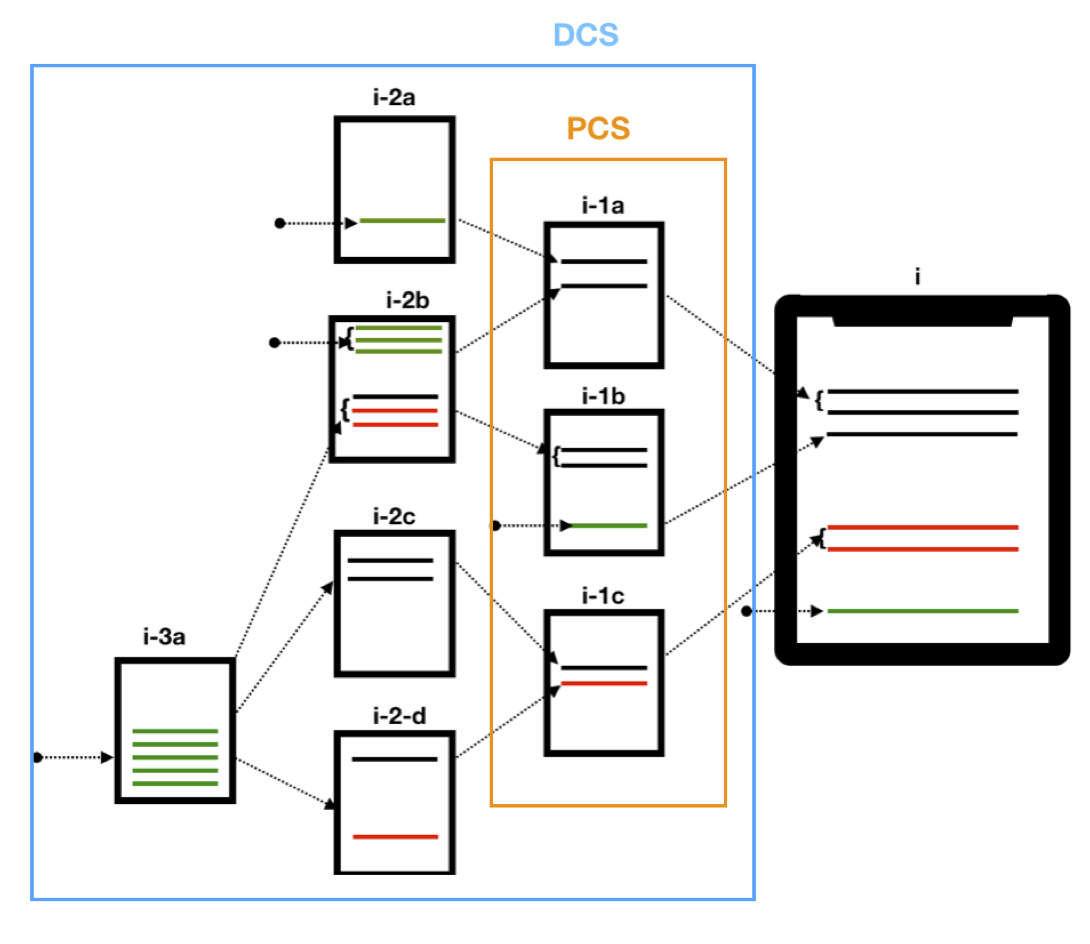
\includegraphics[width=300pt,height=300pt]{img/visiontree.png}
\caption{Genealogy tree of the observable change $i$, each commit shows a precedence relationship its descendant commits.}
\label{fig:genealogytree}       % Give a unique label
\end{figure}


When focusing on commits in the \emph{master} branch of a project repository we do not have a clear visual access to the genealogy tree of a given commit, but we have a flatten version of all the ancestor commits of a given commit. In this flattened version, the commits are preceded by other changes making up a lineal vision of precedence, where the commits of the genealogy can be found. An important concept is that this precedence is not set by dates, but by previous versions in the SCM. This occurs due to the way in which a decentralized source code management (DSCM) system works. Bird \emph{et al.} explained how the local repositories of two collaborating developers working with git might diverge, which causes that each repository to contain new commits that are not present in the other. Thus, in the moment of combining both local repositories, the user can select between many options regarding the sequence of commits such as to rebase, merge, remove, squash, etc. These actions may alter the natural order of commits, which inhibits them from being sorted in time~\cite{bird2009promises}. Continuing with the above example, Figure~\ref{fig:precedence} demonstrates the lineal vision of precedence of the change $i$ in the \emph{master} branch of a project repository. The commits are represented by circles, and the changes belonging to the genealogy tree of $i$ can be found in orange, based on whether they are a $pc$ in blue, or whether they are a $dc$; the remaining commits are the $ac$ where the commit before a $is$ is the immediately ancestor commit $iac$. The \ACSet{i} were committed to the project; however, they do not have a precedence relationship with the lines modified in $i$.    

For those who are familiarized with \texttt{git}, we can compare the Figure~\ref{fig:genealogytree} with the \texttt{git blame} of the modified lines in a bug-fixing change and Figure~\ref{fig:precedence} with the \texttt{git log} of a given commit in the master branch of a project repository. 

\begin{figure}[ht]
\centering
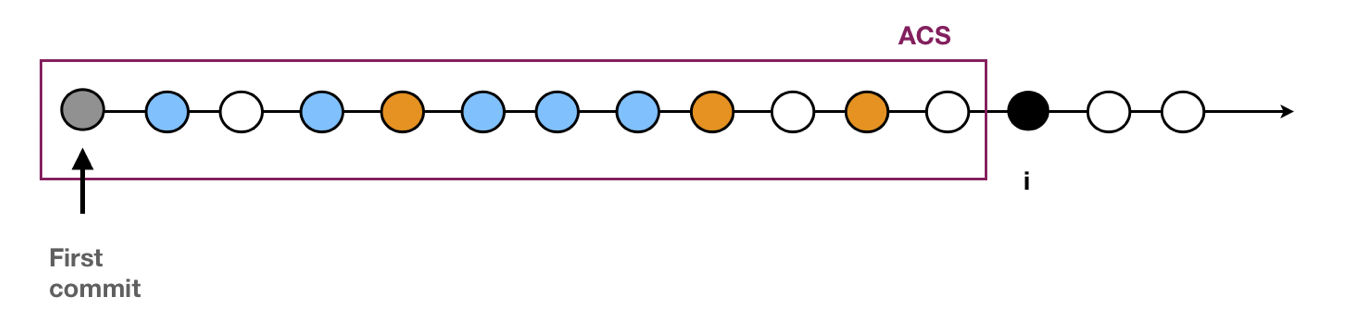
\includegraphics[width=\columnwidth]{img/visionlog.png}
\caption{Lineal vision precedence in the master branch of the bug-fixing change $i$. The colored commits belongs to the \PC{i} (orange) and \DCSet{i} (blue), the black commit is the \BFC and the gray commit is the initial commit of the project. Notice that the commits are not sort in time because we are not assuming a precedence set by dates.}
\label{fig:precedence}       % Give a unique label
\end{figure}

From an objective point of view, it is not important \emph{WHEN} the bug was inserted in time but, \emph{WHAT} commit inserted it. This is because after inserting the erroneous lines in a previous commit or an ancestor commit of a \BFC, the bug is in the system and furthermore, it propagates through each new change in the file. Hence, determining the first failing change that manifests the bug implies to navigate back into the genealogy tree. Thus, from a theoretical point of view, there will be one change in the lineal vision precedence that manifest the malfunction by first time. This change will be the first failing change, and will be referred as \FFC. Furthermore, the \FFC may be the bug introduction change based on whether it inserted the buggy line(s) and whether it belongs to the \ACSet{\BFC}; when there is no change that inserted the wrong line(s) the \BIC in the \ACSet{\BFC} cannot be found, as a result the \FFC is used to explain that in this precise commit, other (external/internal) changes that do not belong to the \ACSet{\BFC}, affected in somehow a line(s) of the source code caused the failure of the system and the bug manifestation.


\section{How to Find the Bug Introducing Change and the First Failing Change:}
\label{sec:findFFCBIC}

In order to discover the Bug-Introducing Change with the maximum accuracy, it is recommended to do it manually by tracking back each line of the source code of all changes of a \BFC until find the \emph{moment} where the bug was inserted by first time. To ensure that it is the moment when the bug was inserted, it is necessary to use information from the code review system and version control system. If according to this information, the commit inserted the line(s) contains the bug at this moment, the change is regarded as \BIC. On the contrary, if the information gathered from these systems explains that there was a change in the \emph{environment or context} that caused the failure, it is not a \BIC, and in this case the change is the First-Failing Change. 

Theoretically and under optimal conditions, this process can be fully automatic relying on the Test Signaling a Bug (\TSB) which flags as \emph{True} when the test is passed and \emph{False} when the test fails in the analyzed snapshots of the project. Despite the high complexity of automating, there is an easy way to find the \BIC or \FFC in this model, which can be achieved through looking manually for the first snapshot in the lineal vision precedence when the \TSB fails. This snapshot submitted the commit that is the perfect candidate to be the \BIC or the \FFC. 

This model focuses on the cases when a \BIC for a \BFC can be found or the cases when it is sure that a \BIC for a \BFC does not exist. To simplify, we assume that there is only the master branch in the repository of a project. To show how the model works, the definitions of \BIC and \BFC based on the existence of a \TSB are applied. The \TSB is applied in all the snapshots of the lineal vision precedence of a \BFC to identify whether there is a Bug-Introducing Commit. Considering that the \TSB  has a coverage of 100\% and that it can run indefinitely across the history of the source code, the proposed model is able to find out the \BIC or the \FFC of a bug report by analyzing the changes that fixed the bug. This \TSB will be passed into all the ancestor commit set of the Bug-Fixing Commit. Thus, when the \TSB test is passed to all the snapshots, it looks for the snapshot that fails; if found, the model will consider it as a candidate for the \BIC. 

To be noted, in previous studies the researchers used software testing to locate faults, however, they were not looking at the origins of the faults by understanding their reasons and their dependencies that may cause the problem that a clean line can become to be buggy in the future. They usually are focused on minimize the cost that a fault may cause in the system by guiding developers to the faulty location, and they do not try to rebuild the complete history of the system in each moment to know what was happening at that moment as our model proposes. Thus, to our knowledge, this is the first time that this idea is presented, where the software testing can be used to find the \BIC and the \FFC using the \TSB.

\subsection{Outcome of the Test Signaling a Bug}
\label{subsec:outcomeTSB}

As mention earlier, the Test Signaling a Bug (\TSB) checks for the functionalities and features of a project with coverage of the 100\%.  Currently,  a common practice in the bug fixing process is to add a test case that checks the behavior of the bug fixed when submitting the \BFC. Thus, the proposed model may use this information from the test case to build the Test Signaling a Bug.

The outcome of the \TSB varies depending on each snapshot, there are three different outcomes:
\begin{enumerate}
	\item {\textbf{Pass}}: The function or feature tested is present in the snapshot and it works as the test anticipated according to the \BFC. The snapshot do not present a \BIC.
	\item {\textbf{Fail}}: The function or feature tested is present in the snapshot but it does not work as the test anticipated according to the BFC. This snapshot is considered as candidate to be the \BIC.
	\item {\textbf{Not-Runnable}}: The function or feature tested is not present in the snapshot, thereby the test cannot run in this snapshot. 
\end{enumerate}

There are three different scenarios to illustrate how to apply the hypothetical test into a lineal vision of precedence for the \setBFC{i} in order to identify whether the Bug-Introducing Commit exists. In these scenarios it is considered that the \TSB have 100\% of coverage and that it can run indefinitely across the history of the source code. Thus, the \TSB is passed to all the snapshots (ancestral commit set) in search for the one that fails; if found, it will be consider it as a candidate for the \BIC. %Furthermore, we will be sure if this snapshot is the \BIC by using some heuristics that check that the line(s) inserted by this commit was (were) buggy, otherwise it cannot be considered as the $BIC$.

Figure~\ref{fig:example1} shows how to apply the hypothetical test to the lineal vision precedence when there is a \BIC and the \TSB can be run in all the snapshots. To locate the \BIC, the \TSB is passed into all the snapshots of the predecessor commit set, and the \BIS will be the first that fails (i-1b). It can be known that the \BIS is a \BIC because the snapshot before (i-2c) passes. 

\begin{figure}[ht]
\centering
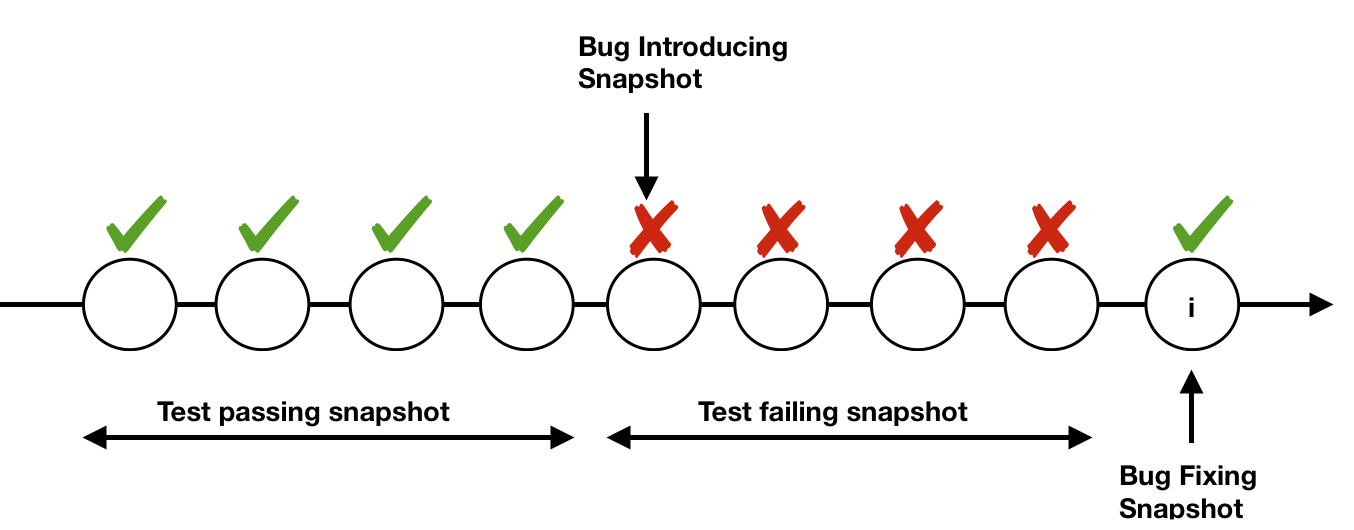
\includegraphics[width=\columnwidth]{img/snapshot1.png}
\caption{The Bug Introducing Snapshot is the \BIC}
\label{fig:example1}       % Give a unique label
\end{figure}

Figure~\ref{fig:example2} shows how  the hypothetical test is applied to the lineal vision precedence when there is a \BIC but the \TSB test cannot be run after a snapshot. This is because the tested function or feature is not present in that moment. Here, the first \BIS identified is the \BIC because when it introduced the function or feature tested, it was buggy.

\begin{figure}[ht]
\centering
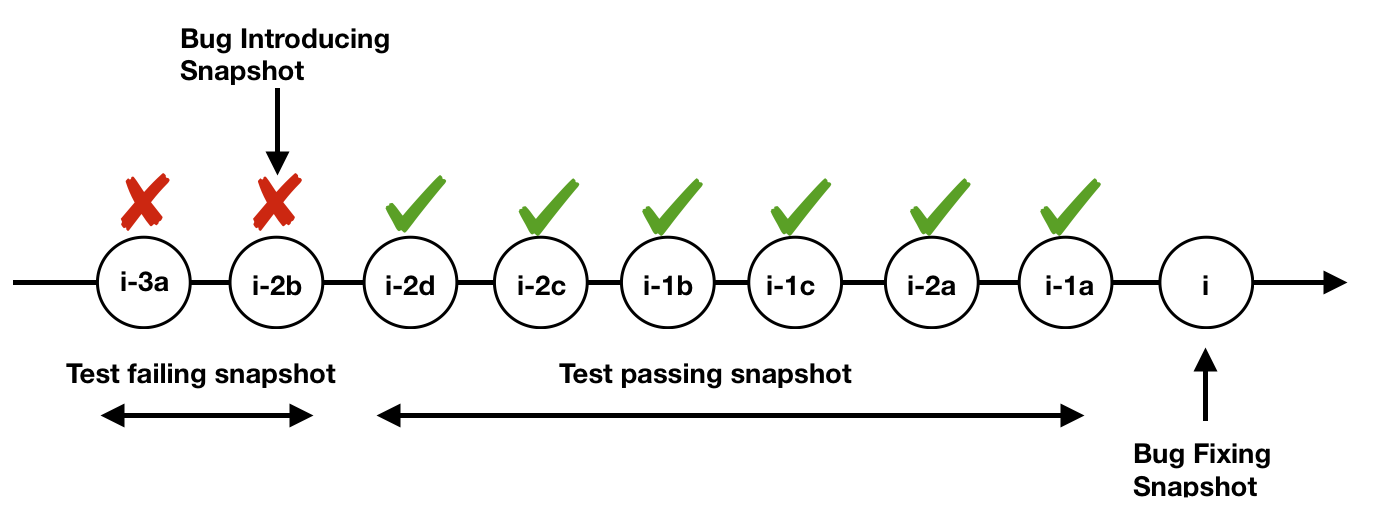
\includegraphics[width=\columnwidth]{img/snapshot2.png}
\caption{The Bug Introducing Snapshot is the the \FFC }
\label{fig:example2}       % Give a unique label
\end{figure}

Figure~\ref{fig:example3} shows how the hypothetical test is applied to the lineal vision precedence when there is not \BIC and the \TSB can be run indefinitely across the history of the source code. The \TSB always fails with the \BFS environment the snapshots, but if the older environment is set, it will pass in the descendant snapshot. Thus, the first \BIS before the \BFC will be the \FFC, there was not \BIC in the predecessor commit set.
\begin{figure}[ht]
\centering
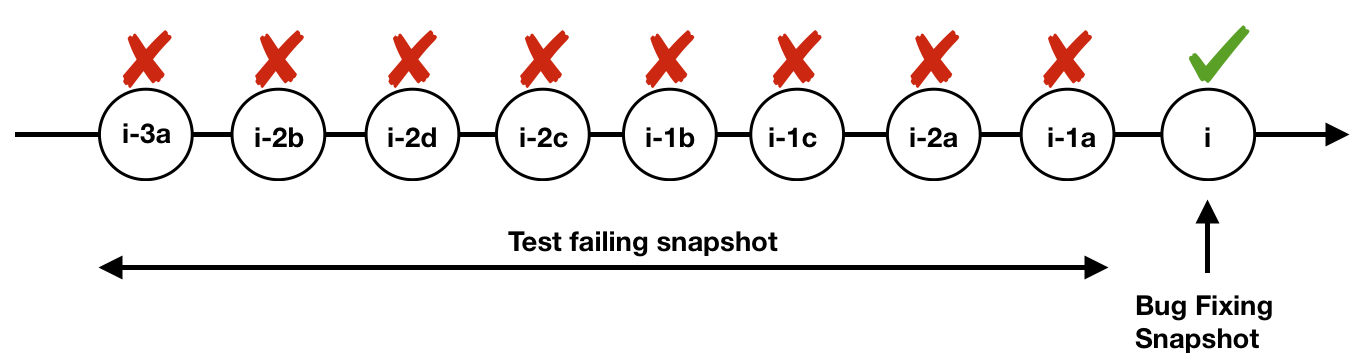
\includegraphics[width=\columnwidth]{img/snapshot3.png}
\caption{The Bug Introducing Snapshot is the the \FFC}
\label{fig:example3}       % Give a unique label
\end{figure}


\subsection{Criterion to apply to the Test Signaling a Bug}
\label{subsec:criterion}

As mention earlier, when the history of a project is linear, researchers can test the \ACSet{i} one by one and run the \TSB.  On the opposite, when the history of the project is not linear, it may have multiple branches to be tested. Furthermore, as the failure might be present in some simultaneously existing branches and absent from other branches the concept of the First-Failing Commit may be uncertain. However, at first glance, and assuming that theoretically the test can be run for all snapshots in the \ACSet{i}, the outcomes of the \TSB still find sections in one or more branches where the test would fail. Thus, the model is still able to find suspicious snapshots to be the \FFC and \BIC. 

It may be possible that in some scenarios, the proposed model should define the \BIC as the one which is topological ``the first one'' in the faction of continuously failing snapshots. It also may occur that, the presence of multiple parallel branches cause two or more commits in parallel start to fail until the \BFC. However, it may be an indication that the bug was introduced into the source code, independently, in several branches or it was copied (or written equally by chance) in several branches. Our hypothesis is that these scenarios are not common, however, we need to include them in the theoretical model.

Thus, to accommodate this case, we could extend the notion of \BIC to ``the set of \BIC'', which would be those ``commits corresponding to the first snapshot to fail, continuously until the \BFC, in several branches that lead to the \BFC''.

Furthermore, depending how the \TSB fails there may be different situations, the researchers should decide whether the \BIS is a \BIC, a \FFC, both, or undecided.

 \begin{enumerate}
	\item \textbf{Undecidable}: When we cannot be sure to find the \FFC or the \BIC. In this class, we may not find the \FFC between all the \ACSet{b} using the hypothetical test because the lack of information.
	\item \textbf{The \FFC is the \BIC}: When we can find the \FFC between all the \ACSet{i} using the hypothetical test and furthermore, this \FFC is the cause of the bug because it inserted the buggy lines to the source code.
	\item \textbf{There is only \FFC}: When the bug was not caused by a change belonging to  the \ACSet{i} but, another external factors cause the failure such as: (1) There is a change in the dependencies of the project; (2) There is a change in the requirements of the project; (3) There is a bug in APIs used in the project. In this class, we will find the \FFC using the hypothetical test and it will be the first time that the malfunction manifests in the project.
	
\end{enumerate}

Nevertheless, it would appear that automatizing this process is tedious and complex, because all the external dependencies used in the project makes it more complicated to build an isolated test to run in each previous change. However, we still rely this can be possible thanks to studies such as the one performed by Bowes~\emph{et al.}, which provides a core list of testing principles that focuses on different quality aspects other than effectiveness or coverage. For our research, the most interesting principle is the test (in)dependency which describes that a test should be able to run in any order and in isolation. In addition, the test should  not  rely  on other tests in anyway. Allowing practitioners to add new tests without keeping in mind dependencies or effects they might have on existing tests~\cite{bowes2017good}.

\section{Algorithm to Find the BIC and the FFC}
\label{sec:algorithmFFCBIC}

Figure~\ref{fig:algoritmo} presents the decision tree in order find the \BIC, whether it exists, and the \FFC. This decision tree is implemented in our model and includes the current shortcomings in the state-of-the-art approaches based on tracking back the lines that have been modified in the \BFC in order to find the \BIC.

 \begin{enumerate}
	\item {\textbf{Lack of guidelines when SZZ identifies more than one pc}}: The decision tree can distinguish when there are more than one previous commit and what needs to be done to identify the \BIC or the \FFC.
	\item {\textbf{Only new added lines in the BFC}}: The decision tree can distinguish when there are only new lines added in the \BFC. In this case, the PC Set is computed by identifying the pc of the lines surrounding the new additions. 
	\item {\textbf{Modifications are not related with the root cause of the bug}}: The \TSB does not test the functions or features that are not related with the root cause of the bug.
	\item{\textbf{ More than one issue are addressed by the BFC}}: The \TSB only implement the test for the functions or features that caused the bug.
	\item {\textbf{Lines correct at the time of their insertion}}: The \TSB always fails with the BFS environment in the snapshots, identifying the \FFC.
	\item {\textbf{Dormant Bugs}}: The \TSB will identify the first snapshot in which the test fails, identifying the \BIC.

\end{enumerate}

\begin{figure}[ht]
\centering
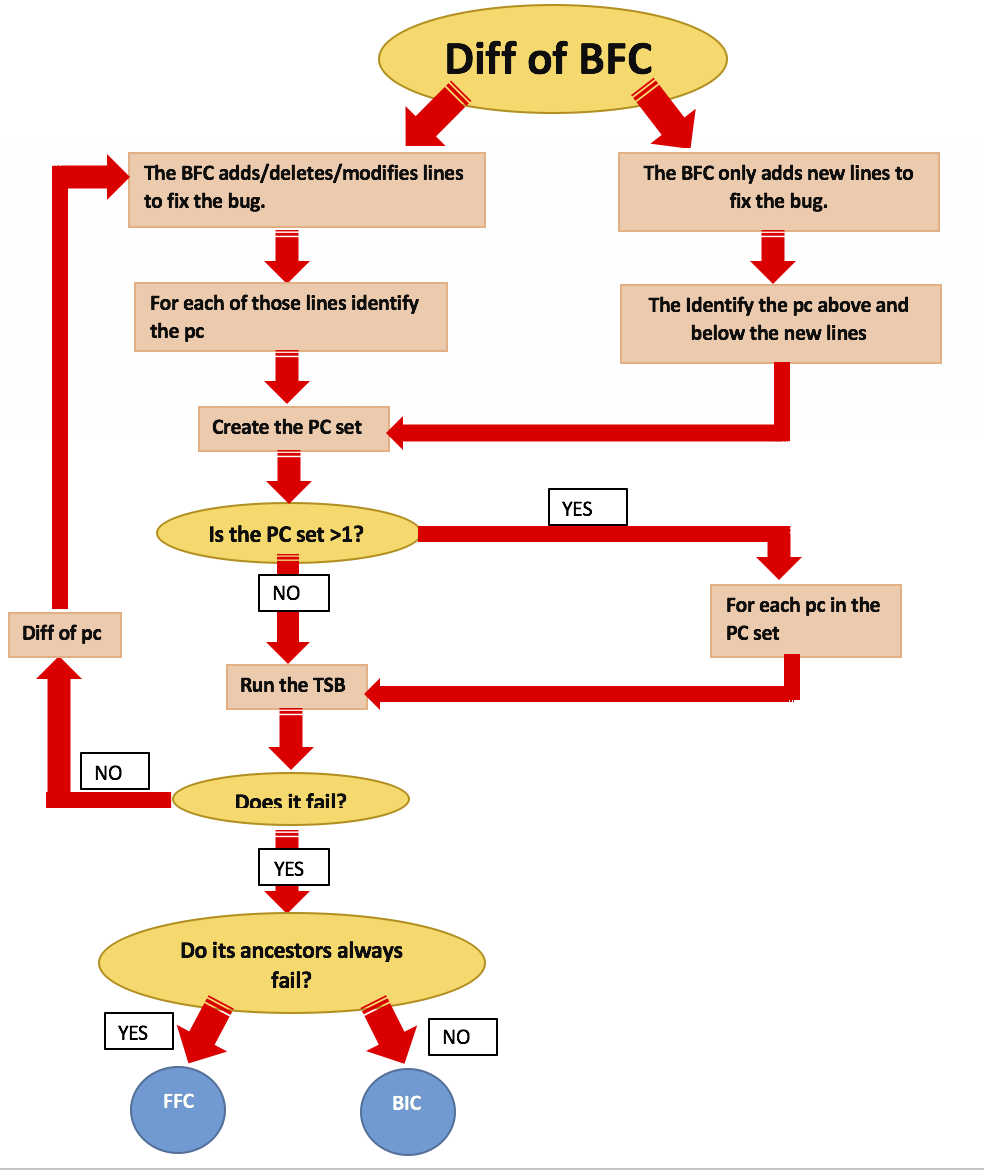
\includegraphics[width=\columnwidth]{img/algoritmo.png}
\caption{Decision tree to identify the BIC and the FFC }
\label{fig:algoritmo}       % Give a unique label
\end{figure}

%%%%%%%%%%%%%%%%%%%%%%%%%%%%%%%%%%%%%%%%%%%%%%%%%%%%%%%%%%%%%%%%%%%%%%%%%%%%%%%%
%%%%%%%%%%%%%%%%%%%%%%%%%%%%%%%%%%%%%%%%%%%%%%%%%%%%%%%%%%%%%%%%%%%%%%%%%%%%%%%%
% APLICATION OF THE THEORY %
%%%%%%%%%%%%%%%%%%%%%%%%%%%%%%%%%%%%%%%%%%%%%%%%%%%%%%%%%%%%%%%%%%%%%%%%%%%%%%%%

\cleardoublepage
\chapter{Empirical Study on the Applicability of the Theory}
\label{chap:application}
This chapter presents an empirical study on the applicability of the theoretical model that was presented before in the Chapter~\ref{chap:Theory}. The empirical study was carried out through analyzing the publicity of available data sources from two OSS projects, Nova and ElasticSearch, and it can be extended to others projects as long as they use VCS and bug-tracking systems. The goal of this thesis is to describe a model to identify unequivocally the bug introduction commit or to determine whether it exists given a Bug-Fixing Commit. Furthermore, this model enables to define the ``gold standard'' to be defined where commits in the repositories are \BIC. 

This chapter is divided into three sections. The first part it is a brief analysis that describes the projects Nova and ElasticSearch and arguments its election as cases of study to identify the origin of the bugs.

The second part clearly defines the methodology to manually analyze and identify the Bug-Introducing Commit given a Bug-Fixing Commit. This methodology explains how the raw dataset has been filtered and details a step by step approach to the stages to identify or discard the \BIC from a specific bug report.  

Lastly, the third part presents the results after applying the model into Nova and ElasticSearch project. The results give more insight into the problem of correctly finding the \BIC by comparing the ``gold standard'' previously identified, with the performance of some state-of-the-art approaches. It computes the \emph{real} false positives and false negatives. %At the end, there is a discussion to confer the impact of the results in the community.  

\section{Case study and datasets}
\label{sec:case}
There are two cases of study that are explained in subsections 6.1.1 and 6.1.2. Both projects have similar characteristics that are interesting and worthwhile to study, but they also have some differences that enables the results to be extended to other open source projects.  

\subsection{Nova}
\label{subsec:Nova}

%We have validated our methodology using the \emph{Grounded Theory}~\cite{charmaz2014constructing} to analyze tickets from two different Open Source projects.
Nova is the most active module of OpenStack project in terms of contributions. OpenStack is a cloud computing platform that is used to build a SaaS (software as a service) with a huge development community thereby making it an interesting project to study. OpenStack has a considerable growth of approximately 350 times in code size and 250 times in number of commits since its first release in November 2009.  Currently, it counts with more than 7,900 contributors, and significant industrial support from several major companies such as Red Hat, Huawei, IBM, HP, SUSE, etc. OpenStack is mainly written in Python. Currently it has more than 328,800 commits with more than 47 million lines of code\footnote{\url{http://stackalytics.com}}. All its history is saved and available in a version control system\footnote{\url{https://wiki.openstack.org/wiki/Getting_The_Code}}, an issue tracking system (Launchpad\footnote{\url{https://launchpad.net/openstack}}) and a source code review system (Gerrit\footnote{\url{https://review.openstack.org/}}).  Table \ref{tablenova} provides a summary of the Nova project. There are 1,602 distinct authors identified in the project from more than 200 different companies. 

 \begin{table}[!t]
\renewcommand{\arraystretch}{0.8}
% if using array.sty, it might be a good idea to tweak the value of
%\extrarowheight as needed to properly center the text within the cells
\caption{Main parameters of the Nova project, June 2018.}
\label{tablenova}
\centering
% Some packages, such as MDW tools, offer better commands for making tables
%% than the plain LaTeX2e tabular which is used here.

\begin{tabular}{|l|c|}
\hline
Parameter & Size \\
\hline
\hline
Companies Contributing &  216 \\
\hline
Commits & 32474 \\
\hline
Contributors & 1602 \\
\hline
LOCs & 4581836\\
\hline
Resolved Bugs &1930\\
\hline
\end{tabular}
\end{table}

In addition to the enormous diversity of people and companies contributing to Nova, the project has other characteristic that make it a good case of study.
\begin{itemize}
	\item \textbf{Research friendly}: Both the bug tracking system and the VCS are a trustful data source for bug-fixing information. In addition, the policy of adding the link of the Bug-Fixing Commit into the bug report information is helpful when linking and analyzing two data sources.
	\item \textbf{The openness of the data set}: all of the data analyzed in this chapter and through the thesis are publicly available. This supports the replicability of the experiments which is a fundamental part of  Empirical Software Engineering.
	\item \textbf{Lineal VCS}: OpenStack policy maintains a lineal history because it uses rebase before the gate accepts commits instead of merging the branches. This makes analyzing Nova efficient since the cases where the bug might be present in some simultaneously existing branches can be reduced.  
	\item \textbf{Programming Language}: Nova uses python as programming language and Python is an interpreted language that do not need to be compiled before running. In addition, Python is dynamically typed which means that the type for a value is decided at runtime and not in advance. These specific characteristics of python might affect the way that bugs are inserted into the source code of a project.
	\end{itemize}

\paragraph{Nova Dataset:}

Launchpad works with issue reports called tickets, which describe bug reports, feature requests, maintenance tickets, and even design discussions. We retrieved randomly 125 closed tickets from Launchpad that were reported during 2015 and had a commit merged into the code source. However only tickets reporting a real bug was studied because it is necessary that a bug exits in order to identify its origin. Thus, to ensure that the tickets describe real bug reports, two different researchers were assigned to analyze them. This is not a trivial task; it is very labor intensive as it has to be done manually. As the task is repetitive, we developed a web-based tool\footnote{\url{http://bugtracking.libresoft.info}} described in Rodriguez \emph{et al.}~\cite{rodriguez2016bugtracking} that helps with the classification process. This tool offers information that is relevant to decide if a ticket is describing a bug report or using information extracted automatically from the project repositories. As it offers a web-based interface, the tool allows for collaboration. Traceability and transparency in the identification of bug reports is also possible as all decisions are stored. 

Each ticket was (manually) categorized into one of following three groups:
\begin{enumerate}
  \item \textit{Bug Report}: The ticket describes a bug report.
  \item \textit{Not Bug Report}: The ticket describes a feature, an optimization/refactoring of the code, changes in test files, or any other situation\ldots but not a bug report.
  \item \textit{Undecided}: The ticket presents a vague description and cannot be assigned without doubts to any of the previous groups.
\end{enumerate}

Subsequently, the tickets agreed\footnote{Please, consider the reading of the paper for further information about the analysis and the ratio of agreement between the researchers}  upon by both researchers as part of the bug report were included into the final dataset. Then, the tickets were linked to their Bug-Fixing Commits.The final dataset counts up to 60 real bug reports that are linked with real Bug-Fixing Commits.

\subsection{ElasticSearch}
\label{subsec:ES}

ElasticSearch is a distributed Open Source search and analytics engine written in Java. It is continuously evolving since its first release in 2010 and currently counts with more than 3,900 commits. This project was  chosen because it has a similar number of commits to OpenStack and its policy of labeling issues is very strict. In the project they use the label ``bug'' to describe issues considered as bug by the developers of ElasticSearch. Thus, researchers can rely on the developers' opinion, and can be sure that the issues retrieved from the issue tracking system are real bug reports and that their Bug-Fixing Commit is fixing a bug. The code of ElasticSearch is hosted in GitHub\footnote{\url{https://github.com/elastic/elasticsearch/}}, and its issue list is available in GitHub\footnote{\url{https://github.com/elastic/elasticsearch/issues}} as well. Table \ref{tableES} provides a summary of the ElasticSearch project. There are 1,000 distinct authors identified in the project and more than 4,500 closed bug reports. 

 \begin{table}[!t]
\renewcommand{\arraystretch}{0.8}
% if using array.sty, it might be a good idea to tweak the value of
%\extrarowheight as needed to properly center the text within the cells
\caption{Main parameters of the ElasticSearch project, June 2018.}
\label{tableES}
\centering
% Some packages, such as MDW tools, offer better commands for making tables
%% than the plain LaTeX2e tabular which is used here.

\begin{tabular}{|l|c|}
\hline
Parameter & Size \\
\hline
\hline
Commits & 39402 \\
\hline
Contributors & 1032 \\
\hline
LOCs & 1187732\\
\hline
Resolved Bugs & 4958\\
\hline
\end{tabular}
\end{table}

In addition to the enormous diversity of people and companies contributing to Nova, the project has other characteristic that makes it a good case study.
\begin{itemize}
	\item \textbf{Research friendly}: The code and the bug reports are hosted in GitHub and it is a trustful data source for bug-fixing information. In addition, the policy of adding the link of the bug report number or the pull request number into the Bug-Fixing Commit is helpful when linking and analyzing two data sources.
	\item \textbf{The openness of the data set}: all of the data analyzed in this chapter and the thesis is publicly available. This helps with the replicability of the experiments which is a fundamental part of Empirical Software Engineering.
	\item \textbf{No Lineal VCS}: Contrary to OpenStack, ElasticSearch repository counts with more than 160 branches with no lineal history. This makes ElasticSearch more complicated to analyze.
	\item \textbf{Programming Language}: ElasticSearch uses Java as the programming language. Java encourages error-free programming as it is strictly typed, performs run-time checks and is independent of hardware. These specific characteristics of Java might affect the way that bugs are inserted into the source code of a project.
	\end{itemize}

\paragraph{Dataset ElasticSearch}: 

ElasticSearch works with issue reports labeled as ``bug'' which discards the necessity of filtering issues that are not describing real bug reports. Thus, since ElasticSearch and Nova have similar amounts of commits, the same amount of closed bugs that are in the Nova dataset are randomly retrieved, with a total of 60 bugs reported during 2015 that have a commit merged into the code source. Then, these bug reports were linked to their Bug-Fixing Commits, thereby the final dataset counts up to 60 real bug reports that are linked with real Bug-Fixing Commits.

\section{Methodology}
\label{sec:methodology}

The methodology used in this empirical study is divided into two parts, the first part is the filtering stage where the researchers ensure datasets fulfill the requirements for analysis under the theory of bug introduction. While the second stage describes each of the steps from the Bug-Fixing Commit until the identification (or not) of the \BIC and the \FFC.

Figure~\ref{fig:diagram} provides an overview of each step involved in our study and their outcomes.

\begin{figure}[ht]
\centering
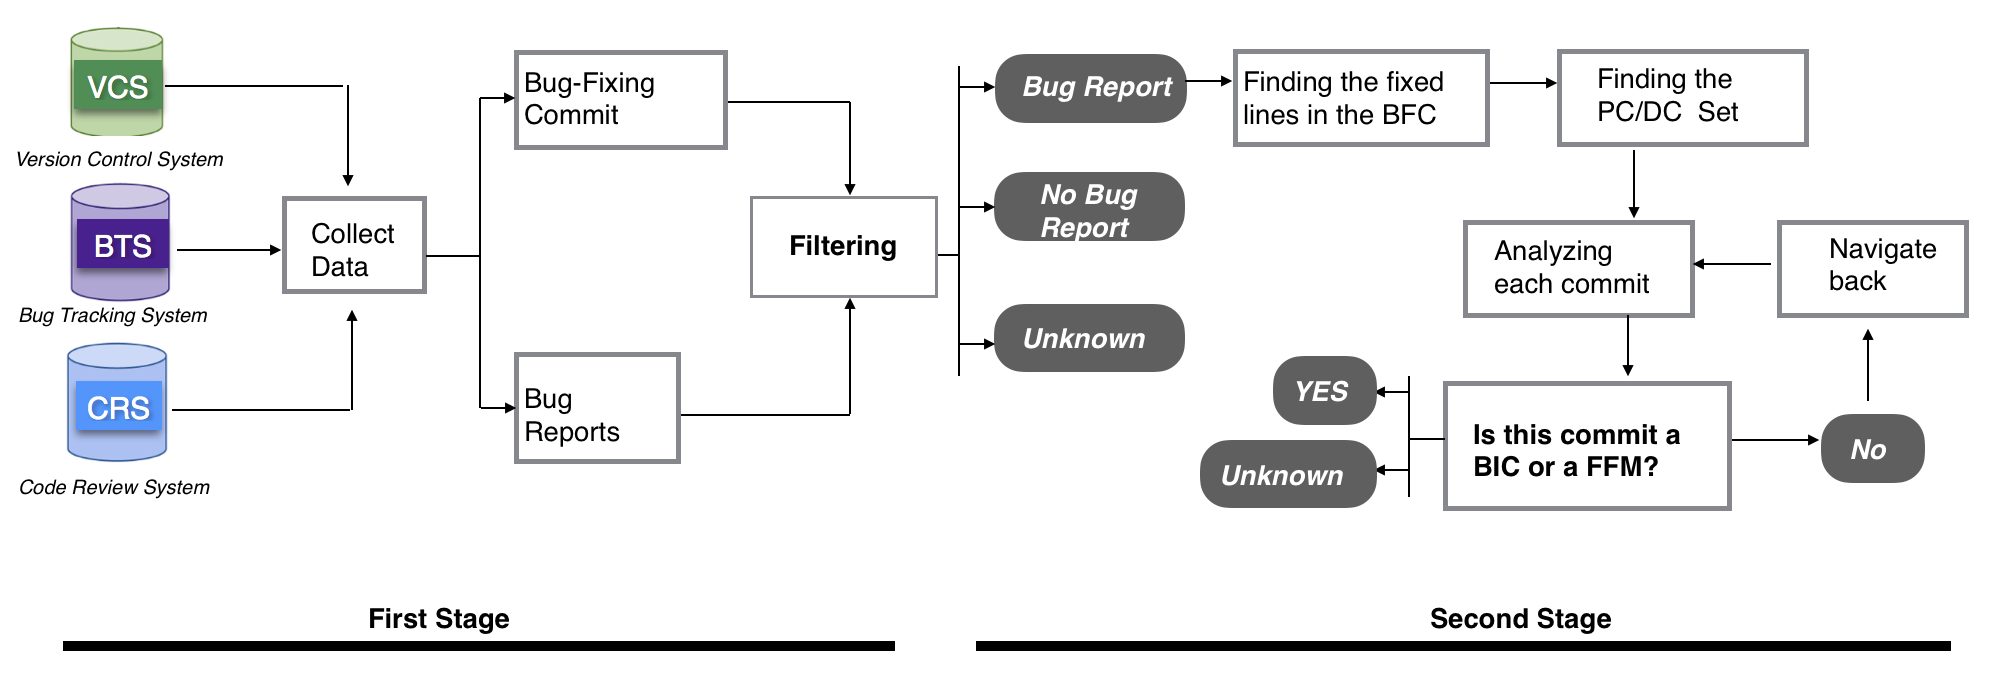
\includegraphics[width=\columnwidth]{img/diagram.png}
\caption{Overview of the steps involved in our analysis }
\label{fig:diagram}       % Give a unique label
\end{figure}


\subsection{First Stage: Filtering}
\label{subsec:methodologyFS}

This stage ensures that the bug reports stored in the datasets can be applicable to our model. Despite the strict policy of bug labeling in ElasticSearch and the agreement on classifying bug reports from other issues in Nova, this stage analyzed carefully each piece of information in the bug reports to ensure the ``gold standard''. Thus, the dataset should only store bugs that are considered bugs at the moment of bug fixing. For example, there is a (hypothetical) test that fails right before the Bug-Fixing Commit and does not fail right after it.  This also ensures that if there are issues that are reported as bugs but are discovered to be new feature requests or improvement suggestions as discussed, they are excluded. 

\subsection{Second Stage: Identifying the First Failing Commit and the Bug Introducing Commit of a bug report}
\label{subsec:methodologySS}

The input of this stage is a set of bug report from Nova and ElasticSearch that describe bugs in the moment of bug fixing. The steps in this stage consists of manually identifying the corresponding Bug-Introducing commit and the First-Failing commit for a Bug-fixing commit, or to decide whether or not there is a \BIC. The identification of \BIC given a \BFC means that the bug was present at the time of committing the lines. Since the \BIC can be in the previous commit or in any of the descendant or ancestor commits, it is necessary to manually analyze them in order to ensure the credibility of the ``gold standard''. In cases where the bug was not present at the time the lines were written, then there is not a \BIC and it becomes necessary to find the \FFC. To better understand this process, the steps are detailed in the following paragraphs. Remember the terminology described in section 5.1.1 that explains concepts such as a the sets of \setBFC{b}, of \PC{b}, of \ACSet{b}, etc. 


\subsubsection{Finding the lines that fixed the bug}

At this stage, the source code that fixed the bug must be identified; a generic bug is referred to as $b$. Therefore, it is important to:
	\begin{itemize}
		\item Identify the change(s) that fixed the bug, \setBFC{b}. In most of the analyzed cases this set was always singleton, meaning that in each bug there is a unique \BFC. However, in the bug report \#1442795\footnote{\url{https://bugs.launchpad.net/nova/+bug/1442795}} there are two different \BFC that fixed the bug. To simplify this process, the methodology assumes that the \setBFC{b} is singleton, and in the case where more than one \BFC fixed the bug, the methodology will analyzed both Bug-Fixing Commit.
		\item Find the lines that the \setBFC{b} touched to fix the bug, \LC{c} where $c$ is the \BFC:
	In the Bug-Fixing Commit linked to a bug report, there is all the information related with the code review process. By applying \textit{``git diff''} it is possible to identify what lines have been added, modified or deleted between the version after the \setBFC{b} and the previous one. There is also the possibility to visualize these changes between the version after the \setBFC{b} and the previous one
 commit using GitHub. GitHub provides a friendly visualization.
 		\item Filter out lines that are not code:
		Lines that have been modified, but do not contain source code (e.g., comments or blank lines) are not considered, and as a consequence they are not analyzed. In addition, there was a \BFC\footnote{\url{https://github.com/elastic/elasticsearch/commit/beaa9153a629c0950182e4e8c4f8eedd1c63f49f}} that closed two different bug reports. In this case, the lines related to the other bug was filtered out.	
	\end{itemize}

\subsubsection{Determining, for each of those lines, \LC{c}, what commit last changed the lines}

Each individual line touched by the \BFC has only one previous commit. However, there could potentially be as many previous commits as modified lines in the \BFC, (see the genealogy tree in subsection 5.1.2). Thus, taking this genealogy tree as reference, the result is a set of all previous commits of the bug $b$, \PC{b}.  

\subsubsection{Analyzing each of these previous commit, and their descendant commits, to determine the \BIC and the \FFC}

This analysis uses information available in the description of the ticket as well as from the logs of the \BFC and commits in the set of \PC{b}. After understanding the bug and the changes that fixed the bug, it is necessary to identify the \BIC and whether it exists, as well as the \FFC.Thus, the identification of the \BIC starts with the analysis of the \PC{b}, for each of the \PC{b} the lines changed are analyzed in order to find which one introduced the bug. At this point, there are three different scenarios and the behavior is different depending on the following conditions:

\begin{enumerate}
	\item \textit{The commit inserted the bug}: This commit is the \BIC because it inserted the buggy lines at the moment of their writing. It was possible to identify the \BIC which is also the \FFC because it is the first commit that manifested the wrong behavior. According to the theoretical model, the \TSB passes in the \BFC and the \BIS is one of the snapshot of a previous commit of the \BFC.
	\item \textit{The commit does not insert the bug}: In this case there will be two possible outcomes:
		\begin{itemize}
			\item The lines in the commit are correct, they do not insert the bug at the time of their writing and other factors caused the lines to became to be buggy. There is no \BIC in this scenario and the analysis should focuses on understanding whether this pc is the \FFC. According to the theoretical model, the \TSB is run in all of the \ACSet{b} and it passes in the \BFC but it always fails in the ancestor snapshots. However, if the environment is changed, the \TSB fails in the \BFC but it passes in the snapshot, and the first \BIS that passes in the sequence of \BIS is the \FFC.
			\item The lines in the commit are syntactic sugar and semantically equivalent modifications (refactoring): This means that the commit retains the same behavior as before, thereby it is required to navigate back into, the \DCSet{b} and start again in the first point of this list.
		\end{itemize}
	\item \textit{It is not sure whether the commit inserted the bug}: In this case it is important to continue navigating back into the \DCSet{b}, if this commit inserted for the first time in the descendant lines of the \LC{c} and it is not certain that they are buggy, the commit is classified as ``undecided''. This means that after the analysis the \BIC was unable to be found manually despite its existence, or their is the case that the \FFC or \BIC was unable to be found due to the lack of context.
\end{enumerate}


\subsection{Outcomes}
\label{subsec:OutcomeES}

At the end of the process there are three possible outcomes for each bug report analyzed. The outcomes are related with the unequivocally identification of the \BIC and \FFC given a \BFC.
These outcomes are explained in the following list:  %\subsubsection{Tickets}

%There are three possible outcomes for each bug report analyzed:
\begin{itemize}
	\item A bug report has a Bug-Introducing Change: In this case it is not sure whether there is at least one bug introducing change among the previous commit set, descendant commit set or ancestor commits set. However, during the manual analysis it may occur that:
		\begin{enumerate}
			\item The moment was able to be identified manually or,
			\item The moment was unable to be identified manually. 
		\end{enumerate}
		Furthermore, in this scenario, the \BIC is also the \FFC.
	\item A bug report does not have a Bug-Introducing Change: In this case, it can be sure that any given line contained the bug when it was committed into the source code, and other factors such as modification in internal resources, changes in external resources, buggy code in third-parties or changes in the requirements that invalidate previous assumptions are the cause of the Bug-Fixing Commit. It can also be confirmed that none of the ancestor commits inserted the wrong lines, thereby none of them can be blamed and only the first time that the bug manifested in the code can be identified. Also, in this case it may occur that:
	\begin{enumerate}
			\item The moment was able to be identified manually or,
			\item The moment was unable to be identified manually. 		\end{enumerate}
	\item It is not clear whether or not a bug report has a Bug-Introducing Change: Some bug reports do not detail enough information about the failure and the Bug-Fixing Commit is not sufficient in deciding whether or not there is a \BIC. Also, some commits are very complex to understand their changes and it cannot be decided whether it inserted the bug or not.

\end{itemize}

\section{Results}
\label{sec:results}
This section presents the results of the empirical analysis in order to locate the \BIC and the \FFC in two cases study, Nova and ElasticSearch. Furthermore, there is a comparison between the results obtained after applying the proposed model with the results obtained with the traditional SZZ algorithm found in the current literature.

\subsection{First Stage}
\label{subsec:resultsFS}

From the 120 bug reports that were classified as bug reports in both projects, 58 from Nova and 58 from ES were considered in the next stage. The main reason was the discordance between the developers to classify them as bug. For example, there are some comments in the bug \#1185290\footnote{\url{https://bugs.launchpad.net/nova/+bug/1185290}} where this discordance is obvious:
	\begin{itemize}
		\item ``I am not sure that I consider this a bug. Without --all-tenants=1, the code operates under your own tenant. That means that --all-tenants=1 foo should really be a no-op without --all-tenants=1.'' 
		\item ``I disagree, mainly because the structure of the requests and code path should largely be transparent to the user. I would suggest that specifying --tenants should imply you are doing a query across --all-tenants=1unless the --tenants specified is the same as what is contained in OS\_TENANT\_NAME (the unless part is debatable)''
	\end{itemize}

Nevertheless, other reasons were also discovered, for instance the bug \#1431571\footnote{\url{https://bugs.launchpad.net/nova/+bug/1431571}} reported a bug in a test file. It was removed from removed  because a bug in a test file does not mean that the source code of the project may contain a bug. It was also discovered that some bug reports such as \#1814\footnote{\url{https://github.com/elastic/elasticsearch/issues/1814}}, \#7740\footnote{\url{https://github.com/elastic/elasticsearch/issues/7740}} and \#1448075\footnote{\url{https://bugs.launchpad.net/nova/+bug/1448075}} are describing hypothetical scenarios. In these cases, the bug description details a possible bug in the future, and they needed to be  removed from the analysis because despite that developers described them to be as bug report, it is understood that at the moment of submitting the Bug-Fixing Commit, the bug was not present in the project. 

\subsection{Second Stage}
\label{subsec:resultsSS}

The main goal of this chapter is to apply the proposed model described in Chapter~\ref{chap:Theory} to identify what are Bug-Introducing Commits, and how they are related to Bug-Fixing Commits. This model enables the ``gold standard'' to be defined where the \BIC in Nova and ElasticSearch correspond with the \BFC. This chapter answers two different questions:

The first part presents the results after applying the model to the data set. Thus, to demonstrate how the model works, we gathered a set of \BFC from two projects, and used to manually identify their \BIC when it exists. As mentioned before, the definitions of \BIC and \BFC were applied based on the existence of a \TSB. In case the \BIC cannot be found, the corresponding \BFC were considered to be removed from the study, since the empirical study is focused in the cases when \BIC can be found or when it is not for certain that it exists.  

The second part presents the effectiveness of a SZZ-like algorithm. Once we have the ``gold standard'', how SZZ-like algorithms ``really'' perform  can be evaluated which is an important contribution to the current literature because as far as can be known, any researcher have carried out this empirical analysis. 

\subsection{Explanation of the Data Sets}
\label{subsec:Explanation}
This section explains the datasets of Nova and ElasticSearch that were manually analyzed to identify the \BIC and the \FFC.

The datasets of Nova and ElasticSearch contains 58 bug reports linked to 58 Bug-Fixing Commit. In Nova there are 9 Bug-Fixing Commits with only new lines added to fix the bug, almost the same number that ElasticSearch which has 8 Bug-Fixing Commit with only new additions. The total number of previous commits identified in Nova was 137 and, 120 in ElasticSearch.   

Figure~\ref{fig:statistic} presents the mean of previous commits, files and test files in each bug report of Nova and ElasticSearch. The mean of previous commits in both projects are around 2, although it is slightly higher in Nova with 2.36 previous commit per \BFC. However, the mean of files touched by the \BFC is higher in ElasticSearch, with a mean of 3.18 files\footnote{the test files are not included here} per bug Report. The mean of test files modified in a \BFC is almost the same in both projects with 1.53 in Nova and 1.60 in ElasticSearch.

\begin{figure}[ht]
\centering
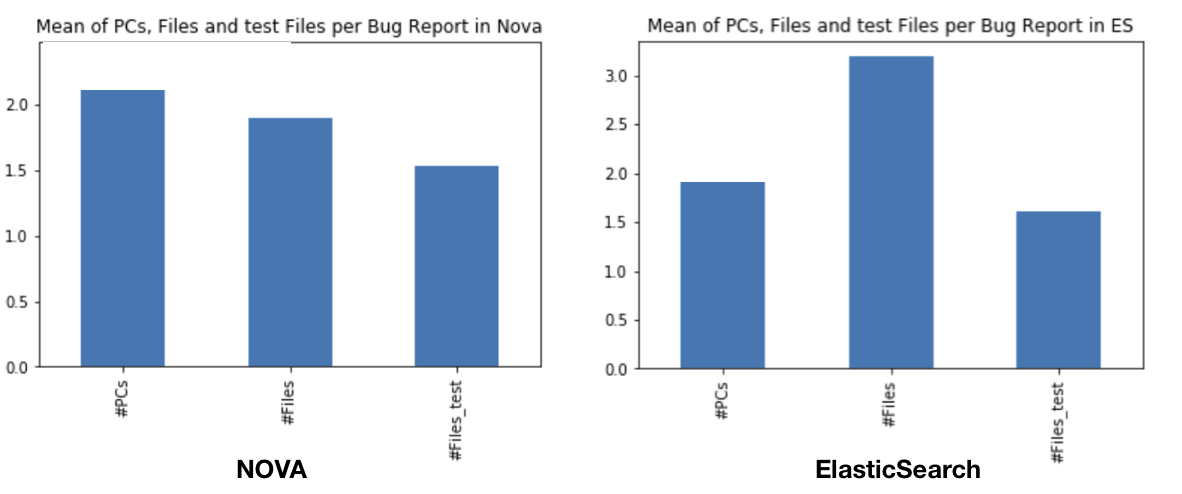
\includegraphics[width=\columnwidth]{img/statistics.png}
\caption{Mean of previous commits, files and test files per Bug Report in Nova and ElasticSearch }
\label{fig:statistic}       % Give a unique label
\end{figure}

\subsection{RQ1: What is the frequency for a Bug-Fixing Commit being induced by a Bug-Introducing Commit?}
\label{subsec:RQ1}

Table~\ref{tableBugNoBug} shows the number of Bug-Fixing Commit that have been induced by a Bug-Introducing Commit and the number of Bug-Fixing Commit that have not been induced by a Bug-Introducing Commit in the datasets.
The trend in the results of both projects was similar as both present higher percentage of Bug-Fixing Commits induced by a  Bug-Introducing Commit. However, the percentage of \BFC that were not induced by a \BIC is more representative in Nova with 24\% of the \BFC being fixing a bug that was not introduced in the system. On the contrary, this percentage is lower in ElasticSearch, where only the 10\% of the \BFC were not induced by a \BIC. Then from the 38 \BFC induced by a \BIC in Nova, 66\% of them were able to be manually located. Whereas from the 45 \BFC induced by a \BIC in ElasticSearch,  80\% of them were able to be manually located. In both projects, the percentage of doubt between where the bug was located is high, with 17\% in ElasticSearch and  31\% in Nova, illustrating the difficulty of the task. 

\begin{table}[!t]
	\renewcommand{\arraystretch}{1.3}
	\caption{Percentage of Bug-Fixing Commit with a Bug-Introducing commit \emph{BIC}, without a Bug-Introducing Commit \emph{NO\_BIC} and Undecided..}
	\label{tableBugNoBug}
	\centering
	\begin{tabular}{|c|c|c|c| }
		\hline
  		&  BIC & NO\_BIC & Undecided \\
		\hline
		\hline
		Nova & 38 (65\%) & 14 (24\%) & 6 (10\%)\\
		\hline
		ES & 45 (77\%) &  6 (10\%) & 7 (12\%)\\
		\hline
	\end{tabular}
\end{table}

\subsubsection{RQ1.1: Which reasons may cause that a Bug-Fixing Commit is not induced by a  Bug-Introducing Commit?}
Additionally, in those cases where the bug report does not present a \BIC, we have looked for its root cause. Table~\ref{tablereasosNoBIC} shows the main reasons for a bug not having a \BIC. 
\begin{table}[!t]
	\renewcommand{\arraystretch}{1.3}
	\caption{ Reasons why a Bug-Fixing Commit is not induced by a bug-introduced commit }
	\label{tablereasosNoBIC}
	\centering
	\begin{tabular}{|c|c|c|}
		\hline
  		& Nova & ElasticSearch  \\
		\hline
		\hline
		Co-evolution Internal & 9 (50\%) & 2 (33\%) \\
		\hline
		Co-evolution External  & 3 (17\%) & 2 (33\%)\\
		\hline
		Compatibility & 2 (11\%) & 0 (0\%)\\
		\hline
		Bug in External API & 4 (22\%) & 2 (33\%)\\
		\hline
	\end{tabular}
\end{table}
Furthermore, they are explained below:
\begin{itemize}
 	\item \textit{Co-evolution Internal}: Changes in the source code related to satisfy the new requirements of the project. Since internal resources have been modified (directory structure and permissions) or requirements have changed invalidating previous assumptions. The bugs caused by the co-evolution internal can be explained from the point of view that the code is not reflecting a new change or requirement of the project and the source code is manifesting the failure.
	\item \textit{Co-evolution External}: Bugs are caused by some external change. External resources have been modified without a previous notification and the source code of the project starts to fail. The bugs caused by the co-evolution external are easiest to understand than the previous ones, because they can be explained from the point of view that a change/update in the source code of an external artifact that the project is using has caused the bug.
  	\item \textit{Compatibility}: Bugs are caused by an incompatibility between software and hardware or an incompatibility with some operating systems.
  	\item \textit{Bug in External API}: A change in the API of a third-party code caused a bug in the source code of the project.
\end{itemize}

These reasons explain why the \BFC was not induced by a \BIC. In Nova the principal reason with a 50\% occurrence rate was the \emph{Co-evolution} of the lines changed to fix the bug with the internal requirements of the projects. The second reason with a 22\% of the cases where the presence of bugs in external APIs that are consumed in Nova. Then,  third most frequent reason is the \emph{Co-evolution} of the lines changed to fix the bug that is related to third-parties code or external artefacts. Finally, the \emph{Compatibility} reasons explain why in 11\% of the cases the \BFC was not induced by a \BIC. On the other hand, in ElasticSearch the percentages are equally distributed with a 33\% occurrence rate in the categories, with the exception that bug caused by the incompatibility of hardware and software were not found. 


\subsubsection{RQ1.2: Could the location of a bug be modeled on the Bug-Introducing moment and First-Failing moment?}

Table~\ref{tableBICFFC} shows the percentage of \BIC and \FFC that have been manually identified by using the model. By definition, and in theory, our model is able to identify the \FFC and the \BIC and whether it exists, but in practice, since the identification needs to be done manually, sometimes the \BIC or the \FFC cannot be identified. To be noticed, these \BFC that were classified into ``Undecided'' in Table~\ref{tableBugNoBug} are not considered in Table~\ref{tableBICFFC} since researcher were not sure whether they have a \BIC or not. Thus, for the 52 \FFC and 38 \BIC belonging to the Nova dataset, 40 \FFC and 25 \BIC were successfully identified.
In the dataset of ElasticSearch, from the 60 \FFC and 45 \BIC, 49 \FFC and 34 \BIC were successfully identified.

\begin{table}[!t]
	\renewcommand{\arraystretch}{1.3}
	\caption{Percentage of Bug-Introduced Commit and First Failing Commits identified after applying the theoretical model.}
	\label{tableBICFFC}
	\centering
	\begin{tabular}{|c|c|c|c|}
		\hline
  		&  BIC & \FFC & Undecided \\
		\hline
		\hline
		Nova & 25 (66\%) & 40 (77\%) & 12 (23\%)\\
		\hline
		ES & 36 (80\%) &  48 (94\%) & 3 (6\%)\\
		\hline
	\end{tabular}
\end{table}

\vspace{0.2cm}
\fbox{\begin{minipage}{30em}
\textbf{RQ1: A Bug-Fixing Commit is not always induced by a Bug-Introducing Commit. The main reasons why a Bug-Introducing Commit is not present in a Bug-Fixing Commit is the co-evolution internal.}
\end{minipage}}
\vspace{0.1cm}

\subsection{ RQ2: What are the specifications that define the effectiveness of an algorithm used to locate the origin of a bug? }
\label{subsec:RQ2}

After applying the model and identifying the number of \BIC and \FFC in our dataset, we obtained the ``gold standard'' where the number of Bug-Fixing Commit with a  Bug-Introducing Commit and without a  Bug-Introducing Commit can be known for certain. For that reason, we are able to compute the true/false positives/negatives for an algorithm, and for that purpose the SZZ-1 algorithm~\cite{kim2008classifying} was selected, an enhancement proposed by Kim~\textit{et al.} of the SZZ. 

The SZZ-1 algorithm does not compute bug-fixing changes with only new lines added, and in the ``gold standard'' of Nova there are three \BFC with only new lines whereas in ElasticSearch there are seven. These cases are the false negatives of SZZ-1. Furthermore, in some \BFC's, the SZZ-1 algorithm identifies more than one possible bug-introduction change. In this case if the \BFC was induced by a \BIC and the SZZ-1 is able to identify it, one true positive and the rest of possible  Bug-Introducing Commit are computed as false negatives. On the contrary, if the SZZ-1 is not able to identify the \BIC between the set of possible  Bug-Introducing Commit, all of them are computed as false positives.  

The ``gold standard'' of Nova consists of 25 Bug-Fixing commits with a  Bug-Introducing Commit and six Bug-Fixing Commits without a  Bug-Introducing Commit. While the ``gold standard'' of ElasticSearch is made up of 36 Bug-Fixing Commit with a  Bug-Introducing Commit and six Bug-Fixing Commits without a  Bug-Introducing Commit. When applying the SZZ-1 algorithm to the set 31 \BFC of Nova, it returns a set of 63 possible  Bug-Introducing Commit. When the algorithm is applied to the 42 \BFC of ElasticSearch, it returns a set of 73 possible  Bug-Introducing Commits. Table~\ref{realSZZ} presents the percentage of true/false positives/negatives for the SZZ-1 as well as the precision and recall.

\begin{table}[!t]
	\renewcommand{\arraystretch}{1.3}
	\caption{Results of True Positives, True Negatives, False Negatives, Recall and Precision for the SZZ-1 algorithm assuming that the algorithm flags all of the commits belong to a set of \PC{b} as \BIC.}
	\label{realSZZ}
	\centering
	\begin{tabular}{|c|c|c|c|c|c|}
		\hline
 	 	&  True Positives & False Positives & False Negatives & Recall & Precision \\
		\hline
		\hline
		Nova & 22 (33\%) & 41 (62\%) & 3 (5\%) & 0.88 & 0.35\\
		\hline
		ES &  26 (33\%) & 47 (60\%) & 7 (9\%)& 0.79 & 0.36 \\
		\hline
	\end{tabular}
\end{table}

In the literature there is no clear heuristic that is followed by researchers when the SZZ identifies a set of possible  Bug-Introducing Commit for a Bug-fixing commit. In Table~\ref{realSZZ} it is assumed that regardless of whether the case occurs, the researchers flag all of the commits belonging to that set as a possible  Bug-Introducing Commit. However, some researchers in the literature state that regardless of whether the case exists, the bug-introduction change is the earlier one in time. With this assumption, the number of true/false positives/negatives of the SZZ-1 is once again computed using the ``gold standard'' of Nova and ElasticSearch. Now, when applying the SZZ-1 to the 31 \BFC of Nova, it returns a set of 28 possible  Bug-Introducing Commit. Furthermore, when SZZ-1 is applied to the 42 \BFC of ElasticSearch, it returns a set of 35 possible  Bug-Introducing Commit. Table~\ref{realSZZ2} presents the percentage of true/false positives/negatives for SZZ-1 as well as the precision and recall in this scenario.

\begin{table}[!t]
	\renewcommand{\arraystretch}{1.3}
	\caption{Results of True Positives, True Negatives, False Negatives, Recall and Precision for the SZZ-1 algorithm assuming that the algorithm only flags the earlier commits that belongs to a set of \PC{b} as \BIC.}
	\label{realSZZ2}
	\centering
	\begin{tabular}{|c|c|c|c|c|c|}
		\hline
 	 	&  True Positives & False Positives & False Negatives & Recall & Precision \\
		\hline
		\hline
		Nova & 21 (68\%) & 8 (26\%) & 2 (6\%) & 0.91 & 0.72\\
		\hline
		ES &  19 (45\%) & 16 (38\%) & 7 (17\%)& 0.73 & 0.54 \\
		\hline
	\end{tabular}
\end{table}

\vspace{0.2cm}
\fbox{\begin{minipage}{30em}
\textbf{RQ2: In the best scenario when applying the heuristics of SZZ-1, Nova computes 26\% of false positives with a precision of 0.72 and a recall of 0.91. ElasticSearch presents higher percentage of false positives (38\%) than Nova, and lower precision (0.73) and recall (0.54).}
\end{minipage}}
\vspace{0.1cm}

\subsubsection{RQ2.1: Which reasons caused that a previous commit identified by the algorithms was not the \BIC?}
Additionally, in those cases where the previous commit identified by the algorithm was not the \BIC, we have looked for its cause. And without being exhaustive, we have identified some of the most common reasons why the previous commits analyzed were not the \BIC, this reasons are following explained:
%Table~\ref{tablereasosNoBIC} shows the main reasons for a commit identified by the algorithm was not the the \BIC. 
%
%\begin{table}[!t]
%	\renewcommand{\arraystretch}{1.3}
%	\caption{ Reasons why a commit identified as previous commit by the algorithms is not the Bug-Introducing Commit }
%	\label{tablereasosNoBIC}
%	\centering
%	\begin{tabular}{|c|c|c|}
%		\hline
%  		& Nova & ES  \\
%		\hline
%		\hline
%		Variable Renaming & 4 (7\%) & 17 (27\%) \\
%		\hline
%		Optimization &  4(7\%) &  2 (3\%)\\
%		\hline
%		API changes &  8 (14\%) &  13 (20\%)\\
%		\hline
%		Obsoleted Code & 13  (22\%) &  7 (11\%)\\
%		\hline
%		Changes done by the \BFC &  9 (16\%) & 25 (39\%)\\
%		\hline
%		Others & 20 (34\%) &  0 (0\%) \\
%		\hline
%		\hline
%		Total & 58  & 64 \\
%		\hline
%	\end{tabular}
%\end{table}
%
%Furthermore, they are explained below:
\begin{itemize}
 	\item \textit{Variable Renaming}: It is a modification in the source code that changed the names of variables. When the algorithms identify a previous commit like this, it means that the line was already buggy or that this change is not related to the bug.
  	\item \textit{Optimization}: It is a modification of the source code to improve code quality and efficiency. When algorithms identify a previous commit commit like this, it means that the bug was already in the logic of the program because the code optimization did not changed the behavior.
  	\item \textit{API changes}: It is a modification in the APIs of the program, normally an the addition of a new argument. When algorithms identify a previous commit like this, and it is not the \BIC, it means that the lines did not contain the bug, but the evolution and necessities of the project make that the line manifested the bug.
	\item \textit{Obsoleted Code}: It is source code that have been useful in the past, but is no longer used. When algorithms identify a previous commit like this, it means that it is not the \BIC because it was removing obsolete code.
	\item \textit{Changes done by the \BFC}: The \BFC may decide to change some parts of the code that are not related to the bug although these lines were clean. 
\end{itemize}



%\gema{el estudio de tokens para los falsos positivos que encontramos en nova y en ES??}

%{RQ sobre como afecta TTN y el BFT y developer en la grand verdad ? }

%%%%%%%%%%%%%%%%%%%%%%%%%%%%%%%%%%%%%%%%%%%%%%%%%%%%%%%%%%%%%%%%%%%%%%%%%%%%%%%%
%%%%%%%%%%%%%%%%%%%%%%%%%%%%%%%%%%%%%%%%%%%%%%%%%%%%%%%%%%%%%%%%%%%%%%%%%%%%%%%%
% DiSSCUSSION %
%%%%%%%%%%%%%%%%%%%%%%%%%%%%%%%%%%%%%%%%%%%%%%%%%%%%%%%%%%%%%%%%%%%%%%%%%%%%%%%%

\cleardoublepage
\chapter{Results and Discussion}
\label{chap:discussion}

This chapter aims to summarize the main results obtained in Chapter~\ref{chap:credibility} and Chapter~\ref{chap:application}. The threats to validity and the potential automation of the theoretical model presented in Chapter~\ref{chap:Theory} is also discussed in this Chapter. 

We first discuss the threats to validity which raise potential questions to answer in the following sections. Then, there are three subsections which present the results and the objectives of this dissertation.

The first subsection presents the results and discussion of the SLR on the credibility and reproducibility of the SZZ algorithm. The importance of this discussion lies on the impact of this algorithm in the empirical software engineering as it has been cited more than 600 times since its publication in 2005.

The second subsection uses the results from the SLR to discuss a theoretical model to identify the change that introduced a bug. This model is mainly motivated by the shortcomings of the SZZ previously identified.

Finally, the subsection discusses the applicability of the theoretical model proposed as well as the implications of the results from the study where this model was applied. The model identifies the Bug-Introducing commit and whether it exists for a given Bug-Fixing Commits based on the assumption of a hypothetical test that can be run indefinitely through the entire history of the software project.  

\section{Threats to validity}
\label{sec:threats}

Wohlin \emph{et al.} claims that there are four main types of validity threats in Empirical Software Engineering research: construct, internal, external and conclusion \cite{wohlin2012experimentation}.

\paragraph{Construct validity}:  This type of threat is in regards to the validity of the metrics used in the empirical research method and whether they claim to be measurable. In the context of this thesis, this validity aspect will focus on the measures and concepts used and the potential problems that may cause bias in the results of the metrics during retrieval.

\paragraph{Internal validity}: Internal validity is the degree to which a causal conclusion based on a study is warranted, which is determined by the extent a study minimizes systematic errors. An attempt was made to minimize this threat by following the procedures for performing SLRs described in ~\cite{madeyski2017would} and by reducing as much as possible the interaction with tools that can introduce bias in the results. Furthermore, replications packages are offered thereby that third parties can inspect our sources.

\paragraph{External validity}:External validity is the degree to which results in this dissertation can be generalized to other contexts. In the empirical study, we selected two case studies: Nova, and ElasticSearch; with its particularities. Thus, this thesis cannot claim that our results can be generalized to other projects. However, researchers should not undermine the value of these case studies.
 
 \paragraph{Conclusion validity}: Conclusion validity is related to how sure the conclusions reached in regards to the relationships in our data are reasonable; this does not affect our approach. 
 
\subsection{Construct validity}
\label{subsec:validity}
Construct validity is the degree to which a research work represents what it is expected to measure. In the context of this thesis: 

\begin{enumerate}
	\item In the Systematic Literature Review: 
		\begin{itemize}
			\item The impact of the SZZ is measured by the number of publications per year that use it. As well as the types and diversity of venues that published these publications.
			\item The reproducibility of the publications that use the SZZ is measured by the availability of a detailed description and data set or of a replication package.  
			\item Since the studies have not been replicated or reproduced in this thesis, the effect on reproducibility is to be considered. However, to mitigate this, an upper limit of publications that may be reproducible are listed.  
		\end{itemize}
	 \item In the Empirical Study: 
	 	\begin{itemize}
			\item TheBug-Fixing Commit is a change that fixed a bug described in a bug report. As mentioned before, there may be cases where commits detected as the fix of a bug turn out to be false because the bug report did not describe a real bug. To mitigate this threat, in Nova the bug reports were analyzed by two researchers to ensure their description was a real bug. Then, in a second round, the obtained dataset was again reviewed to filter out some borderline cases. 
			\item The Bug-introducing commits are the commits that involuntary introduced a bug in the source code. To mitigate the erroneous identification of Bug-introducing commit, they were manually selected by tracking back the fixed lines in a Bug-Fixing Commit. In case of doubt whether a commit is a \BIC or not, it was directly rejected from the final ``gold standard''. 
			\item First-Failing Commits are changes that manifest the failure by the first time. They are identified manually and based on the hypothetical test. However, there may be a possibility where the proposed theory will not work in practice to identify the \FFC. Thus, to mitigate this, in case of doubt, a commit is rejected from the ``gold standard''. 
		\end{itemize}
\end{enumerate}

Hundreds of papers were manually analyzed during the SLR and in the empirical study, thereby human errors might have occurred. The replication packages provided in this thesis do not remove the human errors, but researchers have the possibility to improve and check the work of this thesis.

\subsection{Internal validity}
\label{subsec:internalvalidity}
The internal threats to validity are:

\begin{enumerate}
	\item In the Systematic Literature Review: 
		\begin{itemize}
   		 	\item  There might be a selection bias due to having chosen Google Scholar and Semantic Scholar as the source of all publications on SZZ; other publications may exist that are not indexed by Google Scholar or Semantic Scholar. 
    			\item  There might exists publications that use the SZZ algorithm and not cite the original publication or its improvements. 
    		 	\item The maturity of the field might also affect whether the study has been done in a too early a stage to draw conclusions. However, that more than 10 years is enough time to allow to extract valid lessons from its study.
		\end{itemize}
	\item {In the Empirical Study}: 
		\begin{itemize}
   			\item The limited sample size of bug reports used in this research is the main threat to its validity. There is the possibility that with only 120 seemingly random bug reports, there may be a prior unknown tendency. The probability is relatively high, but there is a long way to obtain a representative sample from a variety of free/open source systems or software projects at large. Our analysis requires a lot of manual human effort, so meaningfully increasing the number of tickets is difficult. However, it should be noted that our numbers are in the order of magnitude of similar studies: for instance, Hindle's \emph{et al.} ~\cite{hindle2008large} article on large commits considered 100 commits, Da Costa~\textit{et al.} ~\cite{da2016framework} article considered to manually analyze 160 bugs as a whole and 80  Bug-Introducing Commits. Finally, Williams y Spacco~\cite{williams2008szz} manually analyzed 25 Bug-Fixing Commits that contained a total of 50 changed lines which were mapped back to a fix-inducing commit.
			\item We are not experts in OpenStack and ElasticSearch projects, and our inexperience may have influenced the results of the analysis when identifying whether a bug was been in the system from the very beginning or whether the code has always been clean. 
			\item A random script was used to extract the tickets from Launchpad and GitHub that have been reported during 2015. There could be unintended bias in the data throughout the course of this year, for instance the phase of the project.
			\item There could be some lax criteria involving the subjective opinion of researchers. To mitigate this, the Bug-Fixing Commit that was not sure was discussed. Furthermore, the ``Undecided'' category was added to mitigate possible false positives from our dataset.
			\item Commits classified into ``Undecided'' group were rejected. There may be the possibility that those commits could have relevant information, and as a consequence, some data that would vary the results.
		\end{itemize}
\end{enumerate}

\subsection{External validity}
\label{subsec:externalvalidity}

The most important external threats, most of them related to peculiarities of the Nova project, are:
\begin{enumerate}
	\item In the Systematic Literature Review: 
		\begin{itemize}
			\item The results about reproducibility using SZZ cannot be generalized to Empirical Software Engineering research because it was a case of study.
		\end{itemize}
	\item {In the Empirical Study}: 
		\begin{itemize}
    			\item The use of diff is the most extended way of providing diff information when looking for the difference between two files. However, other ways of providing diff information are possible.%The use of diff: this is the most extended way of providing diff information when looking for the difference between two files and. Since it works in Git and is implemented in GitHub we use it in this thesis. However, other ways of providing diff information are possible.
   			 \item This thesis only has selected two different programming languages, Java and Python. It is possible that the study of different programming languages turns out in different results.
			 \item The use of the Nova and ElasticSearch as the case of studies implies a better understanding of how bugs appear in these projects. However, Nova and ElasticSearch are projects with a very rapid evolution and a very active community of developers. It could be possible that other projects with fewer commits per year have different results. A higher number of projects would enrich the study.
		\end{itemize}
\end{enumerate}

\section{Discussion}
\label{sec:discussion}

There are three different discussions, based on what has been presented in Chapter~\ref{chap:credibility}, Chapter~\ref{chap:Theory} and Chapter~\ref{chap:application}.

\subsection{Discussion: Reproducibility and Credibility of the SZZ }
\label{subsec:implicationsSZZ}
%This algorithm has been cited more than 600 times since its publication 10 years before, however, there are few studies that provide a replication package even though the researchers of the paper are aware of the limitations and shortcomings of the algorithm.
Chapter~\ref{chap:credibility} details the Systematic Literature Review on the use of reproducibility and credibility of SZZ algorithm. It was demonstrated to be a widely used algorithm in Empirical Software Engineering research. The SZZ is proven to be significantly relevant, and that it is not limited to a niche audience. However, it has become an important component of publications in top journals and prominent conferences in many different topics of Software Engineering. 

During the SLR, it was observed that the limitations of SZZ are well known and documented. Improvements have been proposed, with unequal success up to this moment. The first part of the limitations --related to linking fix commits and bug tracking issues -- has been improved significantly, the enhancements for the second part that has to do with finding the bug introducing change are still limited and accuracy has room for improvement.

Even if limitations have been widely documented, from our study, it can be observed that this has not made ESE practices stronger. From the detailed study of the threats to validity of publications using SZZ, SZZ-1, and SZZ-2, it is clear that most publications are not reporting the limitations, and interestingly enough, limitations to the first part --which have shown to be less relevant-- are discussed more often than the second part. The fact that 38\% of the publications use the \emph{original} SZZ is indicative of this regard. It is therefore recommended for researchers who develop modifications of the SZZ algorithm, to publish the software implementation in development sites such as \texttt{GitHub}, so other researchers can \emph{fork} the project. These \emph{forks} can be easily traced, and the authors will be able to ask for a specific citation to their solution if other researchers make use of it.

The reproducibility of the publications is discovered to be limited, and replication packages are seldom offered. The results presented in our research are in line with previous research~\cite{amann2015software}, although not as \emph{bad} as the ones found for MSR in 2010~\cite{robles2010replicating}. In any case, we think they are not satisfactory enough, and some reflections should be raised on scientific methods used in our discipline.

Even if using one of the improved versions of the algorithm helps with the accuracy of the SZZ approach as pointed out in~\cite{rahman2012clones}: ``Accuracy in identifying  Bug-Introducing Commit may be increased by using advanced algorithms (Kim et al. 2006, 2008)'', they are seldom used and  only 22\% of the publications use one of the two (improved) revisions of SZZ. It seems that researchers prefer to \emph{reinvent the wheel}; 49\% use an ad-hoc \emph{modified} version of SZZ in their publications instead of using other researcher's improvements. One possible reason for this is that papers that describe the SZZ algorithm or any of its improvements do not provide a software implementation. Thus, researchers have to implement it from scratch for their investigation. Our results show that in such a situation, what is often practiced is the adaption of base SZZ algorithm with the addition of modifications, resulting in an 'ad-hoc' solution. For all 'ad-hoc' solutions identified, there is an absence of rationale on why other enhancements to SZZ have not been implemented. Another major problem when using improvements to SZZ is that they have not been given a version/label. Even if a revision of SZZ is used, publications often refer to it as SZZ, making it difficult to follow, to reproduce, to replicate and to raise awareness on this issue.

This thesis provides a simple way to measure the ease of reproducibility and credibility of research papers. Although this measure was formulated only to studies that make use of the SZZ, we think that it can be adapted to other ESE studies easily. Thus, authors can easily assess whether their papers offer a reproducible and trustable work (i.e., with scores above or equal to 5). A Although authors were often addressed directly, the reviewers in the scientific process must not forget their responsibility. It can be observed that authors are often detail-focused when presenting their research; reviewers often have the required vision to evaluate the studies objectively and retains the ability to take these details into consideration. This helps authors to raise the level of their research to another standard. Thus, it is recommended for reviewers to always question the listed points in Chapter~\ref{chap:credibility}  and adapt them to the context of the research when performing a review of a paper which uses heuristics and assumptions..

It was observed that full comprehensive reports on reproducibility are seldom found. Only 15\% of the total analyzed papers are classified as  \emph{good and excellent quality with respect to reproducibility}. The research community should direct more attention to these aspects; we believe that too much attention is put on the final result(s) (the \emph{product} of the research: new knowledge) as opposed to the research process. As researchers in the field of software engineering, we know that both, a high-quality product and process, are essential for a successful advancement for the long term~\cite{kan2002metrics}.

To summarize, it is considered important to highlight some of the lessons learned after performing the SLR. The SZZ algorithm is based on heuristics and assumptions, thus to provide more trustable results, it is recommended for researchers to specify (and argue) the use of the methods/algorithms that mitigate the limitations of their studies. They must also be aware of the risk of every assumption used and, if needed, provide a manual analysis of the results. For studies where the study size is large, researchers can select a random sample to validate it manually. In addition to carrying out empirical studies, the authors must be conscious that the best method to produce reproducible studies is to include a replication package that can be publicly available together with its publication (ideally for an indefinite time). They also have to be aware that some characteristics in their studies, such as software environments, might change, causing both programs and data to become obsolete. As a result, a detailed description of the elements, methods, and software used during the study is also valuable. 

\subsection{Discussion of the Theoretical Model}
\label{subsec:implicationsModel}

Chapter~\ref{chap: Theory} addresses the critical issue of identifying changes that introduced bugs. Currently, the lion's share of the work is based on methods and techniques which rely on the inherently flawed assumption that the lines of code that have been modified to fix a bug are also the lines that previously introduced the bug. While the questionable nature of this assumption is known, this thesis makes an important contribution by detailing a new model to explain how bugs appear in software products. This proposed model does not blame all identified changes as Bug-Introducing Commits, but instead, it searches for when bugs manifest for the first time, and how that can be determined by running a test.

After analyzing many bug reports in this study, we noticed that determining where, when and how a bug is introduced is not a trivial task. There are times where many researchers were involved to clarify the essence of the malfunction. In fact, it is in some cases difficult to even determine whether a bug was present in the code at the time of a given commit's submission. For example, there are cases where the current automatic approaches are unable to determine the point of introduction of a bug, as no previous commit can be identified. One of those cases is when the Bug-Fixing Commit only added new lines in the source code: in such case, there is no way of identifying the previous commit as defined, since there is no previous commit before the addition of lines. In this case, only the description of the ticket or the \BFC could clarify whether the reason for the new lines to be not included lies in some ancestor commit causing the bug, or whether it could be the case that the lines were included in the \BFC to satisfy new requirements or characteristics.

Thanks to the SLR and the in-depth-analysis on the origin of bugs, the limitations, and problems that affect the SZZ-like algorithms when identifying the Bug-Introducing Commits were quantified. Thus, the proposed model integrates these scenarios and is able to deal with them. An explanation of how the model can address each of the limitations is given..
 	\begin{enumerate}   
		\item Identification of more than one previous commit: The model does not focus on identifying the previous commits of the modified lines in a \BFC. It instead tests the behavior of the functionality that was reported as a bug in all the ancestor snapshots of the project to find the first time that the test does not pass.
		\item Scenarios when only new lines are used to fix the bug: The model does not look for lines that have been modified or deleted to fix a bug. It instead considers all the \BFC as it tests the functionality that is failing.
		\item Changes in the environment or configuration: The model can detect bugs caused by changes in the environments using a test that checks whether the functionality that has been fixed in the \BFC and detailed in the bug report behaves correctly with environments of previous snapshots of the project. This means that the hypothetical test will fail when it is running into previous snapshots with the new environment fixed in the \BFC. However, the hypothetical will pass when it is running into previous snapshots with their set environments at this moment. In this scenario, the \BIC cannot be identified since there was any previous change that inserted the bug instead the malfunction was caused by a change in the environment. Consequently, only the \FFC can be found.
		\item Multiple modifications over a line: In our model, it does not matter how many times a line has been modified since it does not blame the last change as the \BIC. The test looks for the first time that the bug was inserted in the line being tested.
		\item Weak semantic level: As in the example above, the proposed model deals with the weak semantic level because it is not focused on identifying the last change; it instead tests the behavior of the code.
		\item Scenarios when a Bug-Fixing Commit fixed more than one bug: In these cases, our model can design a specific test for each defect, looking for the first time that the test fails when testing a bug.
		\item Compatibility reasons: The model identifies the first time that the bug was manifested in the source code using the \TSB to identifies the \BIS.
		\item Dormant bugs: The model identifies the first time that the bug was inserted into the source code using the \TSB. Thus, it does not matter how long the defect had been in the project.
	\end{enumerate}
	
Many researchers have based their methods in locating  Bug-Introducing Commit in the SZZ algorithm or similar algorithms that lack the means to deal with these limitations. They formulate heuristics that for example, remove the \BFC with only new lines to fix the bug because they cannot track back the lines, or they remove longer Bug-Fixing Commits or older commits because they are unlikely to be the \BIC. The consequence is misleading results that have a higher percentage of accuracy when identifying \BIC. 

The SZZ is currently the best-known and easiest algorithm used to identify the \BIC. As a result, some studies may have used datasets to feed their bug prediction or classification models with results obtained from the SZZ such as Ray \emph{et al.} that used a dataset from \cite{rahman2014comparing} which was gathered using the SZZ algorithm to study the naturalness of buggy code. Massacci \emph{et al.} evaluated most existing vulnerabilities of discovery models on web browsers and took many datasets where at least the built-in \cite{massacci2014empirical} used the SZZ approach. And, Abreu \emph{et al.} uses the data set obtained in \cite{abreu2009practical} to study how the frequency of communication between developers affects the fact to introduce a bug in the source code.

	
In general, this new method can distinguish between two relevant moments given a Bug-Fixing Commit, the Bug-Introduction moment and the First-Failing moment. The first moment does not always exist, because there could be external changes or the instance whereby the internal requirements could have evolved which may have caused the failure. However, there is always a First-Failing moment which indicates the first moment when the project manifested the bug. To obtain credible results in areas such as bug prediction, bug categorization, and bug detection, the approaches used to identify when a bug is inserted should distinguish between these two moments, the \FFC and the BIC. The empirical case of study states that the current state-of-the-art approaches only identify from 26\% and up to 38\% of ``real'' false positives. Thus, these results are promising to start thinking about implementing new methods based on the theoretical model proposed in this dissertation, or at least, to consider re-formulating correctly the definition of a bug insertion into the source code. This process cannot be considered as a static problem; the methods proposed might be able to distinguish between buggy lines and clean lines at the moment of its insertion. This dissertation has demonstrated that other external and internal reasons rather than buggy lines are causing the failure of the systems and that it is not fair to blame a change as the cause when in fact, it was correct at that time it was submitted because it fulfilled with the functionalities, environments, necessities, and requirements of the project. Although more  lights have been given to the problem of emulating software faults realistically, to achieve greater bug location automation, a more concerted effort is needed in testing to find ways or techniques to address the re-built problem and to build a test that can be automated or partially automated to find the \BIC or \FFC.

\subsection{Discussion of the Empirical Study Results}
\label{subsec:implicationsES}

The empirical study of Chapter~\ref{chap:application} supports the necessity of a new model to identify the changes that inserted bug as it is not always obvious how errors are introduced into the source code with the current state-of-the-art approaches. This dissertation introduces a new model that could solve this necessity in Chapter~\ref{chap:Theory}. Its implementation has been empirically studied in Chapter~\ref{chap:application}, where the proposed model has been used to carry out a qualitative study on a set of bug reports to identify whether a Bug-Introducing Change exists and, in this case, to pinpoint where it was inserted given a Bug-Fixing Commit.  

The identification of the lines that are responsible for inserting a bug is a quite complicated process. Out of 120 bug reports from the datasets of Nova and ElasticSearch, 116 bug reports with their respective  Bug-Fixing Commit were able to pass to the second stage. In this second stage, researchers manually analyzed whether or not the changes identifies from the \BFC inserted the bug. In both projects, the percentage of changes that introduced a defect into the source code was higher than the others categories, with 65\% of occurrence rate in Nova and 77\% in ElasticSearch. However, the percentage of \BFC that were not caused by introducing a \BIC is more representative in Nova with 24\% of occurrence rate, while in ElasticSearch only the 10\% of the cases.  A possible reason can likely to be attributed to the programming language. While Python is a dynamic language that can run without compilation, Java is strictly typed and performs run-time checks, which may decrease the category of \BFC that were not induced by a \BIC.

During the manual analysis, we discover some reasons which may explain why a \BFC was caused by the insertion of buggy lines. In Nova, the principal reason was the \emph{Co-evolution Internal} with a 50\% occurrence rate, followed by 22\% of the cases where bugs are in external APIs. The third most frequent reason was the \emph{Co-evolution External}, with a 17\% occurrence rate and finally, the less frequent reason was \emph{Compatibilty} with a 11\% of the cases. On the other hand, in ElasticSearch the percentages are equally distributed with a 33\% occurrence rate in the categories, with the exception that bugs caused by the incompatibility of hardware and software were not found. This anecdotal classification should be further investigated since it can help researchers to identify different patterns, probably hidden, which can explain better how bugs are inserted and manifested in the source code.  It also does not claim that these categories can be extended to other projects. We draw attention to the fact that there are other different reasons that cause bugs, and it should be better studied to improve current classifications. To be noted that, although this manual analysis was mostly conducted by the author of this dissertation, in case of doubts, other researchers were involved to discuss and analyze the root cause of the bug.  It may be possible that some differences in judgment about the classification of the root cause exist whether this study is replicated in the future.  In fact, even just determining whether the bug was present at the time when a certain commit introduced the code that latter triggered the error is in some cases not easy.  

After examining several bugs in this study, we notified that attempting to agree on the classification of the root causes of defects is a tedious and sometimes subjective process. Thus, this dissertation suggests an initial classification, without trying to make any strong statement. From the results, it was observed that from 10\% to 24\% of the analyzed \BFC were not induced by a \BIC. Thus, this classification may help to understand better the reasons. 

This dissertation discusses a myriad of options in terms of what a \BIC can and cannot be, and also how an SZZ algorithm will fail, depending on the specific implementation/version of the SZZ algorithm. An essential element of the empirical study is the ``gold standard'', which has the characterizations of \BIC. Thus, the study was able to quantify the ``real'' number of false positives, false negatives and true positives in the performance of the SZZ algorithm, where currently nobody has attempted to calculate before. According to the results presented in Chapter~\ref{chap:application} Section 3.4, in the best scenario, the SZZ computes 26\% of false positives in Nova  with a recall and precision of 0.91 and 
0.72. While in ElasticSearch, the number of false positive increased up to 38\% and as a consequence, the precision and recall decreased with results of 0.73 and 0.54. 
These results may appear to be contradictory with the previous results where ElasticSearch has a fewer percentage of \BFC that were not induced by a \BIC, and it may cause a lower number of false positives than Nova. However, the reason why ElasticSearch computes more false positives is that the presence of \BFC with a \PC set greater than 1 is higher than in Nova. Thus, it explains why the heuristics of the SZZ fail more frequently, and almost in half of these cases. The assumption made about that the earlier commit belongs to the \PC set is the \BIC is frequently wrong in these cases. When there is a \PC set with more than one pc, the SZZ algorithm makes heuristics to identify which commit from the \PC set is the \BIC; in this case, the SZZ algorithm looks for the earlier commit in the \PC set and blames it as the \BIC. Another reason that explains why Nova computes higher recall than ElasticSearch is the number of \BFC with only new lines. This causes the number of false negatives to increase since SZZ does not include these \emph{BFCs} in their analysis.

Other studies such as Kim ~\emph{et al.}~\cite{kim2006automatic}, Williams and Spacco~\cite{williams2008szz}, and Da Costa \emph{et al.} also manually analyzed samples of SZZ data, although they reported much higher percentages of correct SZZ results than this thesis. This is because these studies were not searching for the ``gold standard''; they do not distinguish between \BIC and \FFC, and they do not define what a bug is. As results, they do not contemplate other scenarios which exist and other factors such as changes in external APIs or co-evolution changes. While this dissertation analyzes the whole context of a Bug-Fixing Commit, these articles only focus in verify the bug-fixing hunks, thus they could omit changes in the API or changes due to the evolution of the code. On the other hand, there is also the possibility that the specific projects selected in these studies had a fewer percentage of false negatives due to different cases of bug introduction by previous commits. This is one of the reasons why we propose a further work to extend the analysis to a varied set of projects. 

Our research provides evidence the assumption that the previous commit is where the cause of a bug is located is not true for a significant fraction of bugs. 

In addition, the results also also show that our proposed model theoretically, fulfills with the fundamental concern of identifying unequivocally the \BIC when it exists and that the SZZ, in the best scenario, presents a 26\% of false positives. However, further investigation on the automation of the model needs to be conducted, as well as further study on how external factors and the evolution of requirements affect the manifestation of bugs in the projects.  



%After analyzing several fixing commits in this study, we have seen that real (manually validated) TTN values differ substantially from the ones computed using the well-known and widely-used SZZ algorithm, identifying different BICs for 36\% of the cases in Nova and for 24\% in ElasticSearch. This is the reason why the mean TTN computed using SZZ is almost half the real one.
%The median time to notify a bug is almost 200 days in ElasticSearch and about 350 days in Nova. If we want to calculate the median time of bug fixing for each project, we have to add the median TTF to the TTN, obtaining the BFT. The BFT in ElasticSearch does not differ much from the TTN, whereas in Nova it reaches 400 days. Kim and Whitehead in [11] reported values of BFT that range from 100 to 200 days. In our case studies, only ElasticSearch is in this range, although by very little margin. An explanation for the deviation is because Kim and Whitehead used SZZ to locate the BIC, which we have found is not only always true, but provides an optimistic value.
%
%We have studied the relationship between the variables under study. We have seen for Nova that TTN shows a tendency to increase for lower values of EuBIC, meaning that one of the reasons for high values of TTN could be that the developer who introduced the bug did not have much experience on the project at that moment.
%Given that we have the meta-data from the source code management systems, we could trace how many developers do several tasks in the bug introduction ? > notification ? > fixing process. The results show that notifiers often also fix the bugs. Developers who introduced the bug also appear to fix it (after a third party notifies it) and sometimes they even notify the bug without providing a solution. Interestingly enough, we have found that the number of times where a developer is involved in the three tasks for the same bug report is not negligible. These results raise a lot of questions that are very interesting from the community perspective. One possible reason that explains the low percentage of authors who fix their bugs may be because they are no longer in the project when the bug is reported. We have looked for this and have found that the number of authors who have abandoned the project when the bug was reported was only one in ElasticSearch and two in Nova. This means that other reasons have to be more important than code ownership when it comes to a bug. On the contrary, the high percentages of developers notifying and fixing bugs may be because when they reporting the bug, they already know how to fix it, and this might have and impact reducing the time to fix a bug.
%All in all, we think that the Time To Notify a bug can demonstrate to be a good metric of a project, as it provides good perspective on how the project is maintained. Other metrics can be easily circumvented, as for instance the number of commits or of mailing list messages, and may result in per- verse effects if they are linked with incentives or productivity measures. For TTN (and BFT) this is more difficult to achieve, but not impossible: one could think of a developer introducing a bug and the notifying and fixing it shortly thereafter to obtain lower values.
%Given that one of the problems with TTN (and the rest of associated metrics) is that finding the BIC is difficult and has to be done in a manual way if high precision is the goal, we would like to propose that bug tracking systems include an additional field when closing a bug. In this field, the fixing developer could specify which one was the BIC. It should be noted that there is no one more qualified at this moment that knows where and when the bug was caused. That way the project could have an accurate measure of its maintenance activities and processes, and researchers will access better data and build a better models that estimate effort and the total cost of the software [2], [16], [23].

    
    
%%%%%%%%%%%%%%%%%%%%%%%%%%%%%%%%%%%%%%%%%%%%%%%%%%%%%%%%%%%%%%%%%%%%%%%%%%%%%%%%
%%%%%%%%%%%%%%%%%%%%%%%%%%%%%%%%%%%%%%%%%%%%%%%%%%%%%%%%%%%%%%%%%%%%%%%%%%%%%%%%
% CONCLUSIONS AND FUTURE RESEARCH %
%%%%%%%%%%%%%%%%%%%%%%%%%%%%%%%%%%%%%%%%%%%%%%%%%%%%%%%%%%%%%%%%%%%%%%%%%%%%%%%%

\cleardoublepage
\chapter{Conclusions and Future Research}
\label{chap:conclusions}

This chapter recapitulates the initial research goals and contributions claimed in Chapter 1 and describes the main conclusions of this thesis. Furthermore, the future research is also detailed at the end, in section 8.2.

\section{Conclusions}
\label{sec:conlcusions}

The initial set of research goals and contributions of this thesis introduced in Chapter 1, Section 1.2 and 1.3 were divided into three main sets: 1) The study of the current problem when locating the Bug-Introducing Commit with a SLR based on analyzing articles that employ the SZZ algorithm, as well as the quantification on the limitations of this algorithm. 2) A proposed theoretical model to address more accurately the identification of  Bug-Introducing Commits by distinguishing them from First-Failing Changes. 3) The empirical study on the application of the proposed model in two case studies: Nova and ElasticSearch.  

To understand the problem when identifying the Bug-Introducing Commit, we have performed a case study of ESE practice by means of conducting a SLR on the use of the well-known SZZ algorithm. Our sample of publications consists of 187 publications that make use of the complete SZZ algorithm, out of 458 publications that cite the seminal paper. This SLR sheds some light on some of the problems that ESE research faces when assumptions, as it is the case in SZZ, are made in research methods: publications are primarily non-reproducible, limitations are only occasionally reported, improved versions are seldom used and difficult to identify, and researchers prefer to use their own enhancements. In addition, the SLR also helps to quantify the limitations and problems that affect this particular algorithm when identifying Bug-Introducing Commits: (1) Identification of more than one previous commit, (2) Consideration of scenarios when only new lines are used to fix the bug, (3) Consideration of changes in the environment or configuration, (4) Consideration of multiple modifications over a line, (5) Weakness in semantic level, (6) Consideration of scenarios when a Bug-Fixing Commit fixed more than one bug, (7) Compatibility reasons and, (8) Dormant bugs.

Another key element of this dissertation is the proposed theoretical model that resolves the limitations of the SZZ-like approaches. This thesis defines a bug and how practitioners identify the moment of its insertion by assuming that there exists a hypothetical test that can check the correct behavior of the project in different snapshots. It also provides a criterion that has to be used to apply this model. In addition to the model, we formulate a terminology of different elements and concepts that need to be understood when identifying the change that inserted the bug. To our knowledge, this is the first study aiming to describe a terminology to identify when a bug was inserted given a \BFC.


The empirical experiment demonstrates that a considerable fraction of the analyzed bug reports was not caused by the introduction of buggy lines. The results indicate that factors such as the internal evolution of requirements in the system and external changes and dependencies cause that up to 24\% of the bug reports in Nova and 10\% of the bug reports in ElasticSearch had not a bug introduction moment. The manual analysis facilitates the creation of the ``gold standard'' dataset that was used to compute the real performance of the SZZ algorithm.


To summarize, this thesis focuses on describing and contextualizing the current problem on locating the origin of a bug. To deal with this problem we have quantified the limitations of the most used algorithm, and a solution to these limitations was proposed. The solution introduces a new model to determine how bugs appear in software products. The model was applied to two cases studies: Nova and ElasticSearch to explore how a set of bugs appeared in the projects and how many of them contained ``real'' Bug-Introducing Changes.
 % We have built the ``gold standard'' dataset which was used to compute the real performance of the SZZ approaches.  

% All in all, we have observed that the result is a situation with a lot of room for improvement as excellence in reproducibility is seldom found, and where factors that undermine the credibility of the results are common. We finish by offering some advice in how this situation could be improved in the future, sharing our reflections and stressing the importance of reviewers.


This thesis may present minor modifications of this version. This was done in order to improve the language used. For that reason, please be noted that the last version of this thesis is available at: \url{http://gemarodri.github.io/Thesis-Gema}. 

\section{Future Work}
\label{sec:future}

After manually identifying the Bug-introducing commits and the First-Failing Commits using the criteria detailed in the proposed model, the next logical step is to automatize the  theory as much as possible  in order to find unequivocally the \BIC and \FFC given a Bug-Fixing Commit. As mentioned earlier, there will be some scenarios where the Test-Signaling Bug may be unable to be implemented due to reasons related with the dependencies and the environments used at some previous point in the history of the project. But at least, we should provide different layers of abstraction which describe where and how the \TSB can run. Thus, as future work, I would like to study the extent to which this occurs in an optimal project where all the dependencies would be under control, where each one of the previous environments of the projects can be most likely reproduced. We hope that the automation of the proposed model is also interesting from a practical point of view, because it  would provide software projects with a valuable tool for better understanding what is a bug and how they are introduced, and therefore design measures for mitigation.

Another future line is to select a bigger sample size to carry out a classification to study the frequency with which a Bug-Fixing Commit presents a \BIC depending on the bug report description and the code changed in the line of the Bug-Fixing Commit. This study will provide us with more in-depth knowledge on whether there are patterns that exists which have been hidden in the current literature. This study could help to better design integration tests, to better identify real \BIC or to better check for those cases.

Finally, another interesting future line concerns with the reproducibility and replicability of previous studies based on the use of SZZ-like techniques in order to predict, detect and classify bugs. There is a need for boosting reproducibility and replicability to investigate how it should be addressed by the ESE community, this will help to ascertain the impact of this thesis in other domains as well as the necessity of improving and better defining what is a bug and how it can be located.

%%%%%%%%%%%%%%%%%%%%%%%%%%%%%%%%%%%%%%%%%%%%%%%%%%%%%%%%%%%%%%%%%%%%%%%%%%%%%%%%
%%%%%%%%%%%%%%%%%%%%%%%%%%%%%%%%%%%%%%%%%%%%%%%%%%%%%%%%%%%%%%%%%%%%%%%%%%%%%%%%
% APPENDIX %
%%%%%%%%%%%%%%%%%%%%%%%%%%%%%%%%%%%%%%%%%%%%%%%%%%%%%%%%%%%%%%%%%%%%%%%%%%%%%%%%

\cleardoublepage
\appendix
\chapter{Replicability of the Results}
\label{app:replicability}

Some authors such as Shull \emph{et al.}~\cite{shull2008role} and Basilli \emph{et al.} \cite{basili1999building} have dealt with the task of Mining Software Repositories \emph{MSR}.  This is a complex task because of the high amount of time spent, the necessity of developing some specific tools and the management of datasets. Furthermore Robles ~\cite{robles2010replicating} has raised some questions related with this problem in the ESE.

In first place, there are several elements that may be of interest for reproducibility:

\section{SLR}
\label{sec:replicabilitySLR}
\paragraph{Original data source:} The original data sources used along this thesis can be found in \url{http://gemarodri.github.io/Thesis-Gema} or along Chapter 2, Section 3.
\paragraph{Extraction methodology:} The methodology is briefly detailed in Chapter~\ref{chap:credibility}, section 3. While the scripts created and needed can be also found at \url{http://gemarodri.github.io/Thesis-Gema}
\paragraph{Study parameters:} The initial filter applied over the raw data set is detailed in Chapter~\ref{chap:credibility}, Section 3. 
\paragraph{Results dataset:} The results can be found in Chapter~\ref{chap:credibility}. In addition, they are also available at \url{http://gemarodri.github.io/Thesis-Gema}
\paragraph{Persistence:} it is expected to have access to the website as long as GitHub exists. 

\section{Empirical Study}
\label{sec:replicabilityEmpirical}
\paragraph{Original data source:} The original data sources used along this thesis can be found in \url{http://gemarodri.github.io/Thesis-Gema} or along Chapter~\ref{chap:application}, Section 1.
\paragraph{Extraction methodology:} The methodology is briefly detailed in Chapter~\ref{chap:application}, Section 2. While the scripts created and needed can be found at \url{http://gemarodri.github.io/Thesis-Gema}
\paragraph{Study parameters:} The initial filter applied over the raw data set is detailed in Chapter~\ref{chap:Theory}, Section1 and Section 2. 
\paragraph{Results dataset:} The results can be found in Chapter~\ref{chap:application}, Section 3. Furthermore, they are also available at \url{http://gemarodri.github.io/Thesis-Gema}
\paragraph{Persistence:} it is expected to have access to the website as long as GitHub exists. 


%%%%%%%%%%%%%%%%%%%%%%%%%%%%%%%%%%%%%%%%%%%%%%%%%%%%%%%%%%%%%%%%%%%%%%%%%%%%%%%%
%%%%%%%%%%%%%%%%%%%%%%%%%%%%%%%%%%%%%%%%%%%%%%%%%%%%%%%%%%%%%%%%%%%%%%%%%%%%%%%%
% APPENDIX %
%%%%%%%%%%%%%%%%%%%%%%%%%%%%%%%%%%%%%%%%%%%%%%%%%%%%%%%%%%%%%%%%%%%%%%%%%%%%%%%%

\cleardoublepage
%\appendix
\chapter{Resumen en Castellano}
\label{app:resumen}
\section{Introducci\'on}
 
Los sistemas de software siempre han contenido errores, la b\'usqueda de estos errores ha ocupado y ocupar\'a gran parte de las tareas diarias de desarrollo y mantenimiento de los desarrolladores de software. Los sistemas de software se encuentran en continua evoluci\'on con cambios continuos en el c\'odigo fuente, y adem\'as se hayan vuelto m\'as complejos a lo largo del tiempo, ya que necesitan manejar una cantidad significativa de datos, integrar m\'odulos de terceros y ejecutar multiplataformas. Como consecuencia, desarrollar y probar sistemas de software es actualmente un gran desaf\'io para los ingenieros de software.
% la industria necesita comprender c�mo se introducen para minimizar la posibilidad de que se introduzcan.

Por lo tanto, los defectos son inevitables en alg\'un momento, aunque es com\'un usar algunas t\'ecnicas para detectarlos y prevenirlos con anterioridad, la tasa promedio de defectos arreglados en la industria cuando se trata de crear software es de aproximadamente de 1 a 25 errores por cada 1,000 l\'ineas de c\'odigo \cite{mcconnell2004code}. Esto revela la necesidad de comprender c\'omo se introducen los errores en el c\'odigo fuente para minimizar la posibilidad de que se introduzcan en los sistemas de software. Esto hace que sea especialmente importante comprender los procesos que llevan a la introducci\'on de errores, la manifiestaci\'on de errores y su posterior arreglo. La mejor pr\'actica para entender c\'omo se insertan los errores  en el c\'odigo fuente se basa en el estudio de sus informes, causas y soluciones. Espec\'ificamente, el estudio de los cambios que arreglan un error es un interesante ejercicio  que permite a los investigadores comprender la importancia de entender como se introducen errores en diferentes \'areas de Ingenier\'ia de Software. Por ejemplo, determinar por qu\'e y c\'omo se introduce un error puede ayudar a identificar otros posibles cambios que introducen errores \cite{sliwerski2005changes, kim2006automatic, zimmermann2006mining, thung2013automatic, sinha2010buginnings}; puede ayudar a descubrir patrones de introducci\'on de errores que podr\'ian conducir al descubrimiento de m\'etodos para evitarlos \cite{nagappan2006mining, zimmermann2007predicting, hassan2009predicting, hassan2005top, kim2007predicting}; puede ayudar a identificar qui\'en es el responsable de insertar el error, que tiene el potencial de ayudar en el autoaprendizaje y los procesos de evaluaci\'on por pares \cite{izquierdo2011developers, da2014unveiling, ell2013identifying}; puede ayudar a comprender cu\'anto tiempo est\'a presente un error en el c\'odigo, lo que permite la evaluaci\'on de calidad \cite{rodriguez2017much, chen2014empirical, weiss2007long}, y as\'i sucesivamente. Debido a estas razones, este campo de estudio ha estado activo durante las \'ultimas d\'ecadas.

Hay mucha informaci\'on sobre c\'omo se informan y se gestionan errores en los sistemas de seguimiento de errores, como Bugzilla, Launchpad o Jira. Esta informaci\'on proporciona una descripci\'on textual sobre los \emph{s\'intomas} del error, as\'i como los medios para reproducirlos o enumerar los m\'odulos afectados por el error. Esta informaci\'on se puede vincular al sistema de c\'odigo fuente que proporciona el \emph{tratamiento} mediante cambios en el c\'odigo fuente para corregir el error.

Aunque hay mucha informaci\'on disponible, realmente encontrar cu\'ando se introducen los errores es dif\'icil, hasta el punto de que no est\'a claro c\'omo definir \emph{`` Cu\'ando ''} que se introduzca un error. El t\'ermino, \emph {`` error ''} no se encuentra claramente definido, por lo que los investigadores simplemente est\'an adoptando suposiciones actuales que se encuentran presentes en la literatura. Estas suposiciones establecen que las l\'ineas modificadas para corregir el error probablemente sean la causa de dicho error. Debido al uso general de esta suposici\'on, muchos investigadores no han invertido tiempo en realizar un estudio que profundice m\'as sobre las causas de los errores ya que es una tarea compleja y en ocasiones prefieren mejorar las heur\'isticas usadas bajo estas suposiciones. 

Sin comprender que significa tener un error en el sistema y c\'omo se introduce, es dif\'icil desarrollar un enfoque exitoso para identificar cu\'ando se inserta un error en el software. Es particularmente importante aclarar que nuestra definici\'on de error considera que un error solo se introduce en un sistema cuando se introducen l\'ineas defectuosas en el c\'odigo fuente. Y el momento en que se inserta el error se debe distinguir del momento en que un sistema manifiesta el error por primera vez. Aunque ambos momentos pueden ser iguales, el momento de la introducci\'on del error se puede identificar mediante el uso de una prueba de test hipot\'etica que verifica si el c\'odigo en el momento de su escritura presenta los \emph{s\'intomas} descritos en el informe de error, por tanto:
\begin{itemize}
	\item Cuando falla la prueba, significa que las l\'ineas conten\'ian errores en este momento, y podemos estar seguros de que el error se insert\'o en el momento en que se insertaron las l\'ineas.
	\item Cuando pasa la prueba, significa que las l\'ineas estaban limpias en este momento y que en ese momento no hubo un momento de introducci\'on de errores. Esto se debe a que un sistema tiene diferentes necesidades en diferentes puntos a lo largo del tiempo y los requisitos del sistema cambian y es posible que no se administren adecuadamente; por ejemplo, una l\'inea limpia insertada en el momento \emph{A} puede no causar la falla del sistema, pero cuando el sistema alcanza el momento \emph{B}, la l\'inea puede desencadenar el error que causa la falla del sistema. Esto es posible porque el sistema usa dependencias externas que habr\'an cambiado entre el momento \emph{A} y \emph{B}. Otra posible explicaci\'on ser\'ia que alguna biblioteca externa contiene un error que se insert\'o en el momento \emph{B}. Una tercera explicaci\'on ser\'ia debido a la evoluci\'on del sistema que provoc\'o cambios en otras partes del c\'odigo, afectando as\'i al c\'odigo fuente en el momento al alcanzar el momento \emph{B}.
\end{itemize}

Adem\'as, otros factores tambi\'en complican el desarrollo de un enfoque exitoso para identificar el primer momento de falla del sistema. Por ejemplo, cuando varias modificaciones sobre la misma l\'inea podr\'ian encubrir la verdadera evoluci\'on de una l\'inea de c\'odigo, ocultando as\'i la causa del error \cite{servant2017fuzzy} o cuando solo hay nuevas adiciones de l\'ineas para arreglar el error \cite{da2016framework}. Por otra parte, los enfoques pueden disminuir la precisi\'on cuando los cambios que se arreglan no son modificaciones no esenciales \cite{herzig2013impact} o cuando un cambio no est\'a relacionado con las l\'ineas del c\'odigo que solucion\'o el error \cite{german2009change}.

En la actualidad, muchos investigadores solo han realizado estudios para identificar el cambio que insert\'o el error a trav\'es de tracear las l\'ineas modificadas que corrigierion el error. Sin embargo, este enfoque es ineficaz respondiendo a preguntas relevantes como son \emph {``�qu\'e caus\'o el error? ''} y \emph {``�esta l\'inea era err\'onea en el momento de su inserci\'on? ''}. Porque hasta el momento, no se ha encontrdado ning\'un modelo significativo que pueda validar si la l\'inea identificada, por uno de los m\'etodos actuales, conten\'ia el error cuando se insert\'o en el c\'odigo fuente.


Para investigar y comprender mejor c\'omo aparecen los errores en los productos de software, esta tesis presenta un modelo que define el cambio de c\'odigo que introdujo un error. Este modelo tambi\'en establece la distinci\'on necesaria entre el momento de introducci\'on del error y la primera vez que el error se manifesta en el sistema. Estos momentos no solo se enfocan en estudiar el \emph{tratamiento}, sino que tambi\'en analizan los \emph{s\'intomas}. Siguiendo la evoluci\'on de las  l\'ineas que se han cambiado para corregir el error, el contexto y la historia del error puede ser m\'as f\'acil de entender, y por lo tanto es te\'oricamente posible descubrir si las l\'ineas modificadas para corregir el error introdujeron el error o por el contrario, para confirmar que existen otras razones diferentes a la introducci\'on de l\'ineas err\'oneas que provocaron la aparici\'on del error en el sistema. El conocimiento de esta informaci\'on puede ser muy \'util en muchos campos de la ingenier\'ia de software. Por ejemplo, al calcular varias m\'etricas, como el tiempo que se tarda en notificar un error ~\cite{rodriguez2017much} o la experiencia del autor y su actividad en el proyecto \cite{izquierdo2011developers, izquierdo2012more}. Adem\'as, permite mejorar t\'ecnicas avanzadas que aprovechan dicha informaci\'on para aprender patrones de estos cambios, para motivar el dise\~no y desarrollo de mejores mecanismos \cite{harris2010transactional}, o para ayudar a automatizar predictores de errores que estiman la probabilidad de que dado un cambio, \'este inserte errores \cite{rao2011retrieval, thung2012extent, zimmermann2007predicting}.

%Cuando se ha notificado y posteriormente arreglado un error en el c\'odigo fuente de un sistema, no es f\'acil identificar que cambio previo indujo el posterior arreglo. Actualmente, los desarrolladores tienen a su disposici\'on multitud de informaci\'on almacenada en sistemas webs y sistemas de control de versiones sobre un determinado error y las acciones que se han realizado para su arreglo.
%
%Por un lado, existen aplicaciones web basadas en el seguimiento de errores como por ejemplo, Bugzilla, Launchpad o Jira. Estas herramientas almacenan informaci\'on individualizada de cada uno de los errores encontrados en un proyecto, para ayudar a los desarrolladores a entender mejor los s\'intomas y causas de los errores. La infomaci\'on se presenta en forma de \emph{tickets}\footnote{Un ticket se refiere a una etiqueta/entrada describiendo cu\'al es el error}, donde cada uno de ellos presenta una descripci\'on detallada del error, una lista que enumera las partes del proyecto que se encuentran afectadas, las acciones necesarias para reproducir el error y, en ocasiones, tambi\'en se puede encontrar comentarios de diferentes desarrolladores que aportan informaci\'on relativa al error. Por otro lado, existen sistemas de control de versiones como Git, SVN o Mercurial, que tienen como prop\'osito llevar un registro de los cambios realizados en los archivos de un programa, y que brindan al usuario informaci\'on espec\'ifica sobre que lineas han sido eliminadas, a\~nadidas o modificadas en cada uno de los cambios realizados en el c\'odigo fuente del programa. Finalmente, las informaci\'ones de ambos sistemas puede ser vinculadas, lo que permite a un investigador entender cual ha sido el error y que acciones se han llevado a cabo en el c\'odigo fuente para arreglar el error.
%
%Hasta el momento, las t\'ecnicas m\'as habituales usadas por los investigadores para identificar las l\'ineas, que causaron el error se basan en la asunci\'on que ``dado una modificaci\'on en el c\'odigo que arregla un error, las l\'ineas que han sido modificadas o eliminadas son potencialmente causantes de dicho error''. Por lo tanto, si usamos el sistema de control de versiones para retroceder en la vida de dichas l\'ineas, el \'ultimo momento donde fueron modificadas o a\~nadidas, previo al arreglo, se considera como el momento en el que se introdujo el error. Sin embargo, los investigadores no pueden estar seguros sobre la veracidad de los resultados obtenidos tras aplicar estas t\'ecnicas, puesto que no existe un marco comparativo que indique lo que es correcto y lo que no, que pueda ser usado por los investigadores. Adem\'as, tampoco existe una definici\'on clara y concisa de lo que significa introducir un \emph{error}, o de c\'omo definir el \emph{momento} en el que el error se introdujo. Esta falta de definiciones en la literatura actual, ha provocado que los investigadores tengan que asumir que el \'ultimo cambio realizado en las l\'ineas posteriormente arregladas, fue el cambio que introdujo el error.
%
%Teniendo todo esto en cuenta, esta tesis se enfoca en el estudio de la introducci\'on involuntaria de errores en el c\'odigo fuente. Concretamente, tiene el objetivo de modelar como se introducen los errores no intencionados en el c\'odigo fuente, creando un marco comparativo \'util para comparar el rendimiento de otros algoritmos. Esto es posible ya uqe  ya que \'este marco presenta el ``est\'andar de oro'' donde se han identificado el error y el cambio que lo introdujo. Una de las cualidades m\'as significativas del modelo es la capacidad de distinguir y localizar los dos momentos m\'as importantes para entender como se introdujeron los errores, estos momentos son:
%\begin{itemize}
%  \item El momento de insercci\'on del error: Es el momento en el que un cambio inserta l\'ineas err\'oneas en el c\'odigo fuente de un sistema. En ese mismo momento el error se ha insertado, ya que viola la l\'ogica del sistema.
%  \item El momento de manifiestaci\'on del error: Es el momento en el que un cambio manifiesta el error en el sistema sin la necesidad de que las l\'ineas que est\'en manifestando el error contengan el error. En ocasiones ocurre que las l\'ineas que han cambiado para arreglar el error no fueron err\'oneas en el momento de su introducci\'on por tanto no podemos hablar de ese cambio como el momento de insercci\'on y debemos referirnos a \'el como el momento en el que el sistema manifiesta el fallo por primera vez.
%\end{itemize}
%
%Adem\'as, por definici\'on, el modelo propuesto en esta tesis contempla escenarios que son obviados en el an\'alisis de las t\'ecnicas actuales, como por ejemplo: escenarios d\'onde   \'unicamente se introducen nuevas l\'ineas en el c\'odigo fuente para arreglar el error. Estas l\'ineas no puedes ser rastreadas en la historia previa del proyecto puesto que no exist\'ian anteriormente, y por tanto, las t\'ecnicas actuales descartan estos casos de sus an\'alisis.
%
%La falta de una definici\'on precisa sobre como identificar el momento en el que el sistema manifiesta el error por primera vez y el momento de insercci\'on del error ha dificultado el desarrollo de una t\'ecnica satisfactoria que identifique inequ\'ivocamente cuando un error se introdujo en el c\'odigo fuente y cuando se manifest\'o. Debemos tener en cuenta que cuando nos referimos al ``momento en el que es sistema manifiesta el fallo por primera vez'', no nos estamos refiriendo al momento en el que se report\'o el error o al momento en el que se introdujo el error. Imaginemos por un momento que para arreglar un error se ha modificado la \'linea n\'umero 3 introducida en el momento \emph{A}, si usamos las t\'ecnicas actuales, la causa del error es el cambio que introdujo la l\'inea 3, ese cambio se realiz\'o en el momento A. Sin embargo, si analizamos el contexto de esa l\'inea y sus dependencias, podemos entender que a pesar de ser modificada para arreglar el error, esa l\'inea no introdujo el error en el momento A, si no que hubo un momento posterior, que denominaremos momento \emph{B}, en el que alg\'un cambios externo a nuestro programa, como modificaciones en la API, cambios en nuestro entorno o cambios en terceras partes del c\'odigo han afectado de alguna manera el comportamiento de  esa l\'inea provocando que en el momento B se manifestase el error en la l\'inea 3.
%
%Por otro lado, tambi\'en existen factores que contribuyen a ocultar la verdadera causa del error, como por ejemplo: (i) \'unicamente se a\~naden nuevas lineas para arreglar el error~\cite{da2016framework}; (ii) repetidas modificaciones en las lineas que han sido modificadas para arreglar el error a lo largo de la historia del proyecto dificultan el estudio de la evoluci\'on de esas l\'ineas~\cite{servant2017fuzzy}; (iii) los cambios que arreglan errores, a menudo modifican l\'ineas no relacionados con el fallo~\cite{herzig2013impact}; o (iv) cambios realizados en el  c\'odigo fuente externo a nuestro proyecto causan que algunas l\'ineas de nuestro c\'odigo fuente fallen~\cite{german2009change}.
%
%Para investigar y entender las causas del fallo y su entorno, proponemos un nuevo modelo te\'orico que define un nuevo concepto, el \emph{First Failing Change} \FFC que define el primer momento en el que el software experimenta el fallo. Gracias a este nuevo concepto podemos explicar que, ocasionalmente, el software no falla por un error que haya sido introducido por un desarrollador en un momento concreto, si no que otros factores pueden influir en el fallo, de tal manera que una l\'inea que era correcta se convierta en err\'onea causando el error que fue arreglado posteriormente. Para encontrar el \FFC de un error en el software y entender la historia completa del error, te\'oricamente, navegando hacia atr\'as en las lineas que han sido modificadas por el arreglo, habr\'a un momento en el que el software manifieste el fallo por primera vez, y ese momento ser\'a el \FFC, que puede coincidir o no con el \BIC dependiendo de la naturaleza del error.
%
%En esta tesis, se muestra que hay casos cuando el \FFC no es el \BIC, debido a que el error no fue causado por la insercci\'on err\'onea de la(s) linea(s) por parte de un desarrollador. EL \FFC proporciona contexto al error, algunas veces es f\'acil identificar el momento del fallo tan solo observando la evoluci\'on de las l\'ineas que han sido modificadas para arreglar el error. Sin embargo, otras veces la falta de informaci\'on sobre el error complica el proceso de identificar el momento del fallo.

\section{Antecedentes}

En la literatura existen dos corrientes diferenciadas sobre el estudio de las \emph{causas potenciales} que hacen que los desarrolladores introduzcan los errores. Por un lado, existen t\'ecnicas que se basan en el estudio de los cambios que arreglan un error, espec\'ificamente, identificando las l\'ineas que han sido modificadas para encontrar que cambio previo las introdujo. Sin embargo, las otras t\'ecnicas usadas por los investigadores se basan en el an\'alisis de trazas en el c\'odigo fuente, es decir, estos m\'etodos analizan la asociaci\'on entre los fallos de un programa y la ejecuci\'on de alguno de los elementos de un programa.

A continuaci\'on se describe una breve introducci\'on al estado del arte actual. En el Cap\'itulo~\ref{chap:stateoftheart} se realiza una descripci\'on m\'as detallada.

\subsection{Siembra del error}
\label{subsec:siembra}

\subsection{Identificar el cambio que arregl\'o e error}
Ness y Ngo fueron los primeros en estudiar los cambios que pod\'ian introducir errores, para ello usaron una b\'usqueda simple lineal y binaria, que ten\'ia como prop\'osito aislar el cambio que provoc\'o el arreglo aplicando cambios cronol\'ogicos al programa hasta que la version arreglada presentase el mismo comportamiento err\'oneo que que la siguiente versi\'on del programa~\cite{ness1997regression}. Una de las limitaciones de esta t\'ecnica se produc\'ia cuando un conjunto de cambios provocaba el error, para solventar esta limitacio\'on, Zeller propuso la automatizaci\'on de la t\'ecnica delta debugging, esta t\'ecnica determina el m\'inimo conjunto de cambios que inducen a arreglos~\cite{zeller1999yesterday}.

Purushothaman y Perry midieron la probabilidad, menos del 4\%, de que un cambio peque\~no introdujese errores, nombraron a estos tipos de cambios como \emph{dependencias}, que son cambios en las l\'ineas de c\'odigo que fueron cambiadas por un cambio previo, asumiendo que si el cambio posterior en esas l\'ineas era para arreglar un error, entonces quien lo introdujo fue el cambio previo, ya que era err\'oneo~\cite{purushothaman2004towards}

\paragraph{Cuando existe un cambio que arregl\'o el error (\BFC):}
\'Sliwersky~\emph{et al.} describi\'o como identificar este tipo de cambios en proyectos que usaban sistemas de versi\'on de archivos. Adem\'as propusieron el algoritmo \emph{SZZ}, este algoritmo es uno de los m\'as usados en la literatura actual~\cite{rodriguez2018reproducibility} y se basa en identificar los cambios que arreglan errores para analizar las l\'ineas que han sido modificadas o eliminadas, asumiendo que el \'ultimo cambio realizado en esas l\'ineas antes del arreglo fue el cambio que introdujo el error~\cite{sliwerski2005changes}.

La popularidad en el uso de este algoritmo, provoc\'o que algunos art\'iculos estudiasen como mitigar las limitaciones que presentaba el SZZ. Kim~\textit{et al.} sugiri\'o una nueva implementaci\'on del SZZ que se basaba en la t\'ecnica de \textit{annotation graph} para identificar las l\'ineas que hab\'ian sido afectadas por el cambio que arregl\'o el error. Adem\'as, en este art\'iculo los autores mejoraron la t\'ecnica eliminando del an\'alisis algunos casos como modificaciones realizadas por el \BFC en  l\'ineas en blanco, en los comentarios o cambios del formato~\cite{kim2006automatic}. Por otro lado, Williams y Spacco propusieron una nueva versi\'on del algoritmo SZZ. Esta versi\'on usa diferentes pesos (weights) para mapear la evoluci\'on de una l\'inea. Adem\'as, esta t\'ecnica tambi\'en ignora los comentarios en blanco y los cambios de formato en el c\'odigo fuente~\cite{williams2008szz}. Sin embargo, a pesar de estas mejoras, el algoritmo segu\'ia teniendo limitaciones y segu\'ia identificando err\'oneamente cambios que no causaban errores como los cambios que provocaron el posterior arreglo. Por ese motivo, Da Costa~\textit{et al.} crearon un marco para eliminar del an\'alisis los cambios poco probables de introducir el errores. Este marco se basa en una serie de heur\'isticos como las fechas en las que los supuestos cambios que provocaron el error fueron realizados, las fechas en las que los errores fueron reportados en el sistema, etc~\cite{da2016framework}.

\paragraph{Cuando no existe un cambio que arregl\'o el error:}
La localizaci\'on de errores basada en espectro es una t\'ecnica usada para identificar el origen del fallo. Reps~\textit{et al.} usa \'esta t\'ecnica, cuya entrada es un dos conjuntos de rangos, para ejecuciones exitosas y fallidas, y produce candidatos (l\'ineas, m\'etodos, bloques\ldots) que explica las posibles razones del fallo~\cite{reps}. Abreu~\textit{et al.} investig\'o la precisi\'on de diagn\'ostico en la localizaci\'on de errores como una funci\'on de varios par\'ametros. Sus resultados indicaron que el rendimiento superior de un coeficiente particular es en gran parte independiente del dise\~no del caso de prueba~\cite{abreu2007accuracy}.

Otra de las t\'ecnicas que se usa para localizar el cambio que introdujo el error se denomina el vecino m\'as cercano, en ingl\'es conocido como \emph{Nearest Neighbor}. Renieres y Reiss usaron esta t\'ecnica para localizar el fallo~\cite{renieres2003fault}. La t\'ecnica tiene dos partes principales: En primer lugar, selecciona una \'unica ejecuci\'on fallida y despu\'es, calcula la ejecuci\'on pasada con la mayor cobertura de c\'odigo similar. En segundo lugar, crea el conjunto de todas las sentencias que se ejecutan en la ejecuci\'on fallida pero no en la pasada ejecuci\'on.

Zeller y Hildebrandt desarrollaron por primera vez el algoritmo de Depuraci\'on Delta, m\'as conocido en Ingl\'es como el \emph{Delta Debugging algorithm}, que compara los estados de fallo y \'exito de una ejecuci\'on del  programa, y usa la b\'usqueda binaria para localizar causa del fallo~\cite{zeller2002simplifying}. Desp\u'es, Gupta~\textit{et al.} combin\'o el Delta Debugging
con la t\'ecnica de rebanamiento est\'atico para identificar el conjunto de declaraciones que probablemente contengan c\'odigo defectuoso~\cite{gupta2005locating}. Finalmete, Cleve y Zeller~\cite{cleve2005locating} describieron y usaron la t\'ecnica de transiciones de causa \emph{Cause Transitions} para comparala con el Nearest-Neighbor. Sus resultados sugieren que, bajo el mismo conjunto de sujetos, se comporta mejor la t\'ecnica de Cause Transitions.

\subsection{El uso del Algorithmo SZZ:}
\label{subsec:SZZuso}

%Without trying to be exhaustive, we offer several examples where the authors have used the SZZ algorithm depending on the general purpose. So, Yang~\textit{et al.} apply SZZ to find what kind of  Bug-Introducing Commits are likely to become a great threat after being marked as bug-fixing changes~\cite{yang2014bug}. Zimmermann~\textit{et al.} use it for predicting bugs in large software systems~\cite{zimmermann2007predicting}. Kim~\textit{et al.} show how to classify file changes as buggy or clean using change information features and source code terms~\cite{kim2008classifying}. Kamei~\textit{et al.} apply it to validate effort-aware bug-prediction models [12]. Eyolfson use it to study if time of the day and developer experience affect the probability of a commit to introduce a bug~\cite{kamei2010revisiting}. Yin~\textit{et al.} use SZZ to find how many fixes to bugs introduce new bugs~\cite{yin2011fixes}. \gema{Hablar de bugcache algorithm? -- Predicting Faults from Cached History}

Sin tratar de ser exhaustivos, en esta secci\'on ofrecemos una serie de art\'iculos donde los autores han usado el algoritmo SZZ para diferentes fines. A continuaci\'on se muestran cinco diferentes categor\'ias dependiendo del prop\'osito del art\'iculo en el que se us\'o el SZZ.

\paragraph{Prediccio\'on de Errores}
Feng~\textit{et al.} usaron el SZZ para recolectar datos defectuosos y construir un modelo de predicci\'on de errores universal~\cite{zhang2014towards}. Jiang~\textit{et al.} propuso una nueva t\'ecnica para predecir errores en futuros datos, esta t\'ecnica produce un modelo personalizado para cada desarrollador~\cite{jiang2013personalized}.
Hata~\textit{et al.} desarrollo un sistema de control de versiones detallado para Java, con el finde llevar a cabo predicciones mas exhaustivas. Los autores coleccionaban los m\'odulos err\'oneos usando el algoritmo SZZ~\cite{hata2012bug}. Kim~\textit{et al.} analiz\'o la historia de versiones de siete proyectos para predecir los ficheros y entidades m\'as propensos a errores~\cite{kim2007predicting}. Zimmermann~\emph{et al.}, tambi\'en us\'o el algoritmo para predecir errores en grandes sistemas como Eclipse~\cite{zimmermann2007predicting}. Nagapan \emph{et al.} us\'o el SZZ para predecir la probabilidad nuevas entidades defectuosas tras la distribuci\'on de la nueva versi\'on del software~\cite{nagappan2006mining}. Yang~\textit{et al.} utilizaron el algoritmo SZZ para estudiar la probabilidad de que un cambio que arregl\'o un error, a su vez introdujese otro error en el futuro~\cite{yang2014bug}. Rosen~\textit{et al.} desarroll\'o una herramienta basada en el estudio del algoritmo SZZ que identifica y predice los cambios m\'as peligrosos en el software, ya que pueden provocar errores en el futuro~\cite{rosen2015commit}. Kamei \emph{et al.} introdujeron el concepto just-in-time (JIT) para asegurar una mayor calidad del software, los autores usaron este concepto para construir un modelo que predice si un cambio es probable que introduzca errores~\cite{kamei2013large}.

\paragraph{Clasificaci\'on de errores}
Pan~\textit{et al.} usa varias m\'etricas obtenidas aplicando la t\'ecnica del ``slicing''\footnote{slicing hace referencia a cada una de las ``rebanadas'' del software, esta t\'ecnica es usada para identificar todo el c\'odigo fuente de un programa que puede afectar de alg\'un modo el valor de una variable dada.} para clasificar cambios como err\'oneos o libres de error, los cambios err\'oneos son identificados usando el SZZ~\cite{pan2006bug}. Kim~\textit{et al.} estudi\'o c\'omo clasificar los cambios en archivos como defectuosos o libre de errores usando las caracter\'isticas de los cambios realizados en el c\'odigo fuente para arreglar el error~\cite{kim2008classifying}. Thomas~\textit{et al.} introdujeron un marco dise\~nado para combinar m\'ultiple configuraciones de clasificadores, mejorando de esta manera el rendimiento del mejor clasificador~\cite{thomas2013impact}. Ferzund~\textit{et al.} presentaron una t\'ecnica para clasificar los cambios realizados en el software como libre de errores o err\'oneos, usaban el SZZ para identificar de los trozos de c\'odigo que fueron modificados anteriormente y que introdujeron errores~\cite{ferzund2009software}. Kim y Ernst propusieron un algoritmo de priorizaci\'on de alertas basado en la historia de control de versiones de un proyecto para ayudar a mejorar la priorizaci\'on de herramientas de b\'usqueda de errores. Este algoritmo se basa en SZZ para identificar l\'ineas de archivos relacionadas con errores~\cite{kim2007warnings}.

\paragraph{Localizacion de errores}
Asaduzzaman~\emph{et al.} usaron el algoritmo SZZ en Android para identificar los cambios que introdujeron errores para despu\'es, usar esa informaci\'on y buscar problemas de mantenibilidad del proyecto~\cite{asaduzzaman2012bug}. Schr{\"o}ter~\emph{et al.} construyeron un conjunto de datos para el proyecto Eclipse que contiene informaci\'on sobre los cambios que introdujeron errores y los cambios que arreglaron esos errores~\cite{schroter2006if}. Kim~\emph{et al.} desarrollaron una herramienta para encontrar fallas usando la memoria de los arreglos de errores, este m\'etodo se centra en el conocimiento sobre los cambios que arreglaron los errores. La herramienta usa an\'alisis estad\'istico para aprender patrones de error espec\'ificos de un proyecto mediante el an\'alisis de la historia de un proyecto para luego sugerir correcciones~\cite{kim2006memories}. Wen~\emph{et al.} propusieron otra herramienta para localizar errores basada en la recuperaci\'on de informaci\'on y utiliza el algoritmo SZZ para extraer los cambios que introdujeron errores y evaluar de este modo la herramienta~\cite{wen2016locus}.

\paragraph{Entender la Evoluci\'on del Software}
Kim y Whitehead analizaron los proyectos ArgoUML y PostgresSQL para calcular el tiempo que tarda un error en ser arreglado despu\'es de haber sido introducido en el c\'odigo fuente~\cite{kim2006long}. Tambi\'en, Kim~\textit{et al.} estudi\'o las propiedaddes y la evoluci\'on de los patrones de cambios realizados en siete diferentes sistemas de software escritos en C, usaban el SZZ para identificar los cambios que introdujeron errores~\cite{kim2006properties}. Eyolfson usa el SZZ para estudiar si el momento del d\'ia en el que se introduce un cambio y la experiencia del desarrollado que lo introduce, afecta a la probabilidad de introducir m\'as errores en el c\'odigo~\cite{kamei2010revisiting}. Izquierdo~\textit{et al.} usa el algoritmo SZZ algorithm para estudiar si los desarrolladores arreglan los errores que han introducido~\cite{izquierdo2011developers}, adem\'as, los autores tambi\'en usan este algoritmo para estudiar la relaci\'on entre la experiencia de los desarrolladores y la introducci\'on de errores en la comunidad de Mozilla~\cite{izquierdo2012more}. Rahman y Devanbu estudian los factores que tienen m\'as impactyo en la calidad del software, como la propiedad del c\'odigo, la experiencia, la estructura organizacional y la distribuci\'on geogr\'afica. En este estudio, el algoritmo SZZ se us\'o para identificar las l\'ineas de c\'odigo asociadas con los cambios que introdujeron los errores~\cite{rahman2011ownership}.

\paragraph{Estudios Emp\'iricos}
Nguyen y Fabio Massacci realizaron un estudio para validad la confiabilidad de los datos de la versi\'on vulnerable de NVD. Los autores usaron el algoritmo SZZ para identificar el c\'odigo vulnerable responsable de la vulnerabilidad~\cite{nguyen2013reliability}. Bavota~\textit{et al.} estudiaron emp\'iricamente en qu\'e medida las actividades de refactorizaci\'on introdujeron errores en tres sistemas que usaban Java como lenguaje de programaci\'on~\cite{bavota2012does}. Kamei \emph{et al.} utilizaron el algoritmo SZZ para revisar los modelos de predicci\'on de errores en la literatura~\cite{kamei2010revisiting}. Fukushima \emph{et al.} evalu\'o emp\'iricamente el rendimiento de los modelos de predicci\'on de errores basados en el concepto Just-In-Time~\cite{fukushima2014empirical}.

\section{Modelo te\'orico Propuesto para localizar errores}
Esta secc\'on presenta la definici\'on de un modelo para identificar inequ\'ivocamente los cambios que introducen errores (\BIC). \'Este modelo identifica un conjunto de cambios que introducen errores y que se corresponden con un conjunto de cambios que arreglan errores (\BFC). Adem\'as, este modelo incluye definiciones precisas de lo que significa un \BFC y un \BIC, definiciones basadas en la suposici\'on de que existe una prueba hipot\'etica con una cobertura de test perfecta y que podr\'ia ejecutarse indefinidamente a lo largo de la historia del c\'odigo fuente del proyecto. El modelo propuesto devuelve verdadero o falso dependiendo de si el error estuvo presente o no en un momento espec\'ifico del proyecto, de tal manera que podemos usar la prueba o test para comprobar si una determinada funcionalidad esta presente y se comporta de acuerdo a las expectativas en cada momento de la historia del proyecto. Por primera vez, un modelo contempla diferentes escenarios que han sido excluidos en la literatura actual, por ejemplo, los \BFC que presentan solamente nuevas lineas a\~nadidas, o la distinci\'on entre el momento de inserci\'on y el momento de manifestaci\'on de un error.

El objetivo principal para describir este nuevo modelo es ampliar las t\'ecnicas actuales usadas en la l\'iteratura y garantizar de esta forma que las cambios identificados como responsables de introducir el error en el c\'odigo fuente en realidad introdujeron el error en alg\'un momento de la historia del proyecto. Finalmente, \'este modelo se usar\'a como un marco te\'orico para la evaluci\'on del rendimiento de otras t\'ecnicas en la identificaci\'on de \BIC, as\'i como para comparar la efectividad entre los diferentes algoritmos, ya que junto con el modelo propuesto se define un \emph {``est\'andar de oro''} en que se identifican inequ\'ivocamente que cambios son \BIC en un proyecto. Antes de explicar en detalle la teor\'ia del modelo propuesto, se requiere definir algunos conceptos que sob utilizados para explicar el modelo.

\subsection{Definiciones:}

Buscar el origen del error es una tarea compleja que implica una gran variedad de elementos y conjuntos individuales en su b\'usqueda. De tal manera que, encontramos la necesidad de formular una terminolog\'ia que es una de las partes de valor en esta tesis. Esta terminolog\'ia se puede aplicar a los sistemas modernos de administraci\'on de c\'odigo fuente. La terminolog\'ia define cada elemento y cada conjunto de elementos que tienen lugar durante el an\'alisis para la identificaci\'on del \BIC a partir de un \BFC. Para evitar confusiones, a continuaci\'on se definen los conceptos con los que vamos a trabajar:

\paragraph{\textbf{Cambio at\'omico \emph{(at)}:}} Es una operaci\'on que aplica un conjunto de cambios distintos como una operaci\'on \'unica. En esta tesis, el cambio at\'omico se refiere a un cambio m\'inimo de una l\'inea.
\paragraph {\textbf{Cambio at\'omico anterior:}} Dado un cambio at\'omico $at$, nos referimos a $at'$ como la \'ultima modificaci\'on que cambi\'o la l\'inea $l$ de un fichero $f$. Por lo tanto, la relaci\'on de precedencia entre un cambio at\'omico y su cambio at\'omico previo es la siguiente:
\[ at' \rightarrow at\] 
\paragraph {\textbf{Commit \emph{(c)}:}} Un cambio observable que registra uno o m\'as cambios at\'omicos en el c\'odigo fuente de un sistema de software. Estos cambios generalmente se resumen en un parche que es un conjunto de l\'ineas que un desarrollador agrega, modifica o elimina en el c\'odigo fuente. Los commits actualizacian la versi\'on actual del directorio \'arbol.
\paragraph {\textbf{L\'ineas modificadas:}} Por definici\'on, una confirmaci\'on puede cambiar cero\footnote{se cambian cero l\'ineas cuando solo se agregan nuevas l\'ineas en un commit.} o m\'as l\'ineas de c\'odigo; y nos referimos a ellas como \emph{l\'ineas cambiadas} de un commit y las denotamos como \LC{c}.
\paragraph {\textbf{Precedencia entre commits:}} Relaci\'on entre \emph{cambios at\'omicos} de un commit con sus \emph{cambios at\'omicos previos} en un fichero $f$, d\'onde el commit previo de un commit es el cambio at\'omicos anterior de un conjunto de cambios at\'omicos. Nos referimos a esta precedencia entre commits como \emph{commit previo(\pc)} de una commit en $f$ y la designaremos como:
\[ pc'(c) \rightarrow pc(c)\] 
\ paragraph {\ textbf {Conjunto de commits previos:}} Conjunto que incluye los diferentes commits previos a un commit. Formalmente:% Adem�s, se puede describir como la primera generaci�n de confirmaciones en el conjunto de cambios ancestrales (\ ACS) del �rbol geneal�gico para un \ BFC determinado. Lo denotamos como
\[ \PC{c} =  \bigcup pc'(c)\]

\paragraph {\textbf{Commit Descendiente:}} Dado un commit $c$ y un fichero $f$, una confirmaci\'on descendiente de $c$ es una de las confirmaciones que pertenece a la cadena de commits de precedencia de $c$ en $f$, nos referiremos a \'el como $dc$.
\paragraph {\textbf{Set de Commits Descendientes:}} Conjunto de commits descendientes para un commit determinado; nos referimos a \'el como \DCSet{c}. Debemos tener en cuenta que \emph{set de commits previos} contiene solo los commit previos a un commit, mientras que el \emph{set commits descendientes} contiene todos los commits que han modificado, de alguna manera, las l\'ineas cambiadas en $c$ durante toda la historia del fichero $f$.
\paragraph {\textbf{Ancestor Commit:}} Es cualquiera de los commits anteriores a un commit determinado, nos referiremos a \'el como $ac$.
\paragraph {\textbf{Conjunto de Ancestor Commits:}} Conjunto de los ancestor commits de un commit determinado; lo llamamos \ACSet{c}. Debemos tener en cuenta que a partir de un commit espec\'ifico del repositorio, el \emph{conjunto de ancestor commits} contiene todos los commits de ese repositorio.
\paragraph {\textbf{Inmediatamente Ancestor Commit:}} Es el commit inmediatamente anterior a un commit determinado en el conjunto de ancestor commits, nos referiremos a \'el como $iac$.
\paragraph {\textbf{Instant\'anea o Snapshot:}} Representa el estado completo del proyecto en alg\'un momento de la historia. Usando git como ejemplo, dado un commit $c$, la instant\'anea correspondiente ser\'ia el estado del repositorio despu\'es de escribir en la terminal de comandos ``git checkout c''. La evoluci\'on del software se puede entender como una secuencia de instant\'aneas, cada una correspondiente a un commit, en el orden mostrado por `` git log'' (orden de confirmaciones en la rama considerada).
\paragraph {\textbf{Commit que arregla un error (\BFC):}} Commit d\'onde se solucion\'o un error. Dado un error $b$ se puede requerir uno o m\'as commits para reparar el error, definimos el conjunto de commits que arreglan un error como el siguiente conjunto: \setBFC{b}. En general, esperamos que este conjunto sea \'unico, es decir, que un error se corrija en un \'unico commit, a pesar de que se pueden necesitar varios commits para corregir un error. Adem\'as, un commit que corrige un error solo existe si realmente es un error en el momento de la correcci\'on, porque para descubrir qu\'e cambio introdujo el error, es necesario que el error analizado sea realmente un error.
\paragraph {\textbf{Snapshot de la soluci\'on del error (\BFS):}} instant\'anea del c\'odigo correspondiente a un \BFC.
\paragraph {\textbf{Test Signaling a Bug (\TSB):}} Una prueba utilizada para indicar que hay un error presente. Se define como una prueba hipot\'etica, que se puede ejecutar en cualquier instant\'anea del c\'odigo, devolviendo \emph{True} si la prueba pasa, lo que significa que la instant\'anea no contiene el error, y \emph{False} si la prueba no pasa, lo que significa que la instant\'anea contiene el error. 
\paragraph {\textbf{Prueba que falla en la snapshot \emph{(T-S)}:}} instant\'anea para la cu\'al el \TSB falla.
\paragraph {\textbf{Prueba que pasa en la snapshot \emph{(T + S)}:}} instant\'anea por la cu\'al el \TSB pasa.
\paragraph {\textbf{Snapshot introductor de errores (\BIS):}} Primera instant\'anea en la secuencia continua m\'as larga de T-S, que termina justo antes de \BFS. Es decir, hay una secuencia continua de instant\'aneas para las que falla la prueba, comenzando en el \BIS y terminando justo antes del \BFS. Como la prueba falla desde la instant\'anea hasta la correcci\'on, podemos saber que la prueba fall\'o en esa secuencia y, dado que esta es la primera instant\'anea con el fallo de la prueba, podemos decir que \'esta es la primera instant\'anea ``con el error presente''.
\paragraph {\textbf{Cambio que introdujo el error (\BIC):}} Un commit espec\'ifico perteneciente al \BIS que introdujo la(s) l\'inea(s) err\'onea(s) en el momento de su inserci\'on, y el error se propag\'o en el sistema a trav\'es de los commits posteriores hasta que el \BFC arregl\'o el error.
\paragraph {\textbf{First Failing commit (\FFC):}} El primer commit correspondiente al \BIS que manifiest\'o el error pero que no introdujo l\'ineas err\'oneas en el momento de su inserci\'on.

\subsection{Explicaci\'on del modelo propuesto:}
Con demasiada frecuencia, cuando se analizan proyectos, los investigadores usan \texttt{git} como sistema de gesti\'in de c\'odigo fuente \textit{(SCM)}. El SCM registra \emph{cambios observables} en un archivo o conjunto de archivos. Los cambios observables son alteraciones de archivo(s) causados por adiciones, eliminaciones o modificaciones de una o m\'as l\'ineas en el c\'odigo fuente. Gracias al SCM, los investigadores pueden rastrear de forma manual o autom\'atica la eliminaci\'on y modificaci\'on de l\'ineas desde un momento espec\'ifico hasta su origen, y tambi\'en pueden identificar qu\'e l\'ineas son nuevas adiciones en cada commit. Navegando hacia atr\'as en la relaci\'on entre las l\'ineas alteradas de cada cambio observable y su cambio anterior, se puede construir un \emph{\'arbol de precedencia de cambios observables} o \emph{\'arbol geneal\'ogico}. La figura~\ref{fig:genealogyarbol} muestra un ejemplo del cambio observable $i$ realizado en un ficherp $f$ que corrigi\'o el error $b$. Rastreando cada l\'inea modificada o eliminada de $f$, podemos dibujar el \'arbol geneal\'ogico de las l\'ineas involucradas en $i$. Es importante saber que las nuevas l\'ineas a\~nadidas no se pueden rastrear, pero se tiene en cuenta en el modelo. Los recuadros negros representan los diferentes commits, los puntos representan un conjunto de solo nuevas l\'ineas, las flechas muestran la precedencia entre commits, y el color de las l\'ineas se relaciona con la acci\'on realizada, eliminar (rojo), a\~nadir (verde) o modificar (negro).

Usando la terminolog\'ia definida anteriormente, nos vamos a referir al cambio observable $i$ como el \BFC. A partir de las l\'ineas cambiadas en el \BFC, \LC{\BFC}, podr\'iamos dibujar su \'arbol geneal\'ogico en el que, gracias a la precedencia entre los commits, hay una relaci\'on geneal\'ogica. Visualmente a partir de esta relaci\'on, distinguimos entre commits de la primera generaci\'on \emph{(i-1a, i-1b, i-1c)}, segunda generaci\'on \emph{(i-2a, i-2b, i-2c, i -2d)}, y tercera generaci\'on \emph{(i-3a)} del \BFC. Por extensi\'on, el conjunto de commits previos del \BFC es la primera generaci\'on de commits y el conjunto de commits descendientes es la primera, segunda y tercera generaci\'on de los commits.

\[ \PC{\BFC} =  {(i-1a,i-1b,i-1c)}\]
\[ \DCSet{\BFC} =  {(i-1a,i-1b,i-1c),(i-2a, i-2b, i-2c, i-2d),(i-3a)}\]

\begin{figure}[ht]
\centering
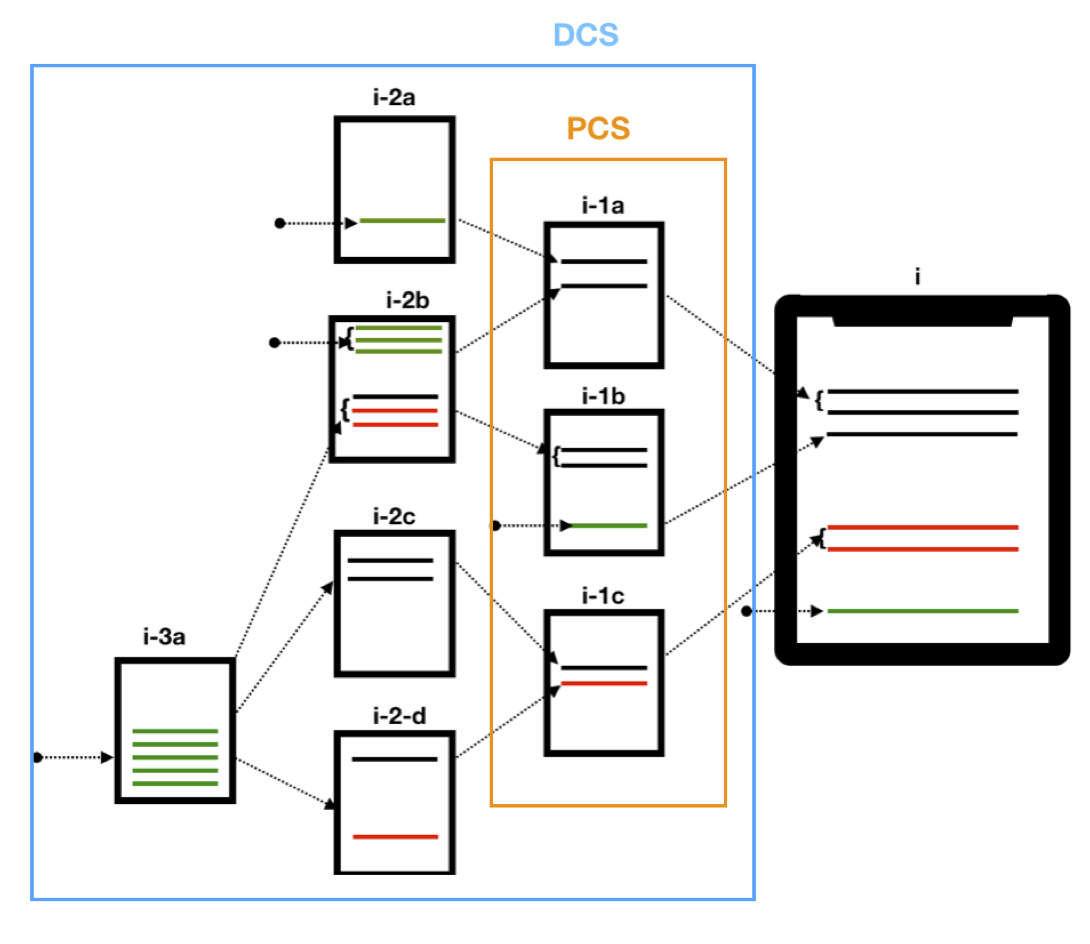
\includegraphics[width=300pt,height=300pt]{img/visiontree.png}
\caption{\'Arbol geneal\'ogico del cambio observable $i$, cada confirmaci\'on muestra una relaci\'on de precedencia con sus compromisos descendentes.}
\label{fig:genealogyarbol}       % Give a unique label
\end{figure}

Cuando se observan los commits en la rama \emph{master} de un repositorio de proyectos, es posible que no se tenga un claro acceso visual al \'arbol geneal\'ogico de una commit determinada, pero se tiene una visi\'on aplanada de todas los ancestor commits  de un commit determinado. En esta visi\'on plana, los commits van precedidos por otros cambios que conforman una visi\'on lineal de precedencia, donde se pueden encontrar los commits geneal\'ogicos. Un concepto importante a tener en cuenta, es que esta precedencia no est\'a establecida por fechas, sino por versiones anteriores en el SCM. Esto ocurre debido a la forma en que funciona un sistema descentralizado de gesti\'on de c\'odigo fuente (DSCM). Bird \emph{et al.} Explic\'o c\'omo podr\'ian divergir los repositorios locales de dos desarrolladores que colaboran a la vez en un proyecto que usa git, lo que hace que cada repositorio contenga commits que pueden no est\'an presentes en el otro repositorio. Por lo tanto, en el momento de combinar ambos repositorios locales, el usuario puede seleccionar entre muchas opciones relacionadas con la secuencia de commits, tales como rebase, merge, remove, squash, etc. Estas acciones pueden alterar el orden natural de los commits, lo que las inhibe de ser ordenados cronol\'ogicamente en el tiempo~\cite{bird2009promises}. Continuando con el ejemplo anterior, La Figura~\ref{fig:precedencia} muestra la visi\'on lineal de precedencia del commit $i$ en la rama \emph{master} del repositorio de un proyecto. Los commits est\'an representados por c\'irculos, y los cambios que pertenecen al \'arbol geneal\'ogico de $i$ se pueden encontrar en naranja si son $pc$ o en azul o si son $dc$; los commit restantes son los $ac$ d\'onde el commit anterior al $i$ es el inmediatamente ancestor commit $iac$. El conjunto de \ACS{i} fueron a\~nadidos al proyecto; sin embargo, no tienen una relaci\'on de precedencia con las l\'ineas modificadas en $i$ y no aparecen representados en la figura.

Para aquellos que est\'an familiarizados con \texttt{git}, podemos comparar la Figura~\ref{fig:genealogyarbol} con el resultado obtenido tras usar \texttt{git blame} en las l\'ineas modificadas en \BFC y la Figura~\ref{fig:precedencia} se correspoder\'ia con el resultado de usar \texttt{git log} en una confirmaci\'on espec\'ifica de la rama principal de un repositorio en un proyecto.

\begin{figure}[ht]
\centering
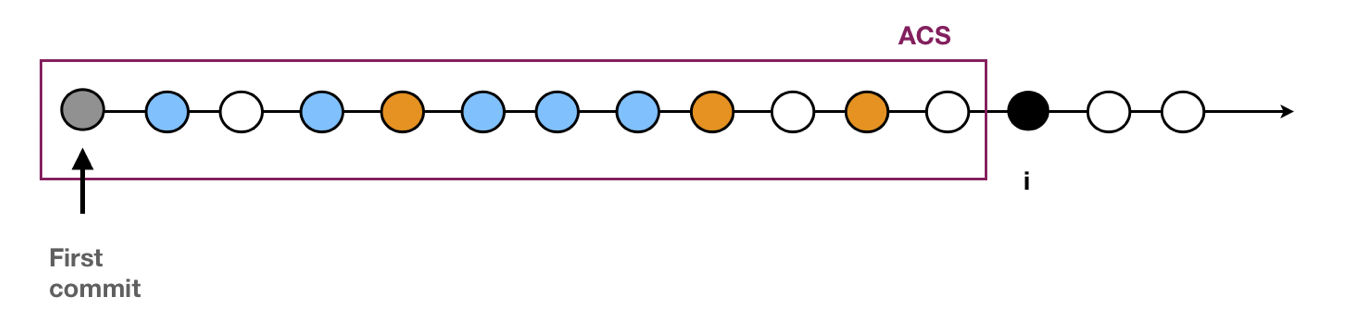
\includegraphics[width=\columnwidth]{img/visionlog.png}
\caption{Visi\'on de precedencia lineal en la rama master del commit que arregla el error. Los commits coloreados pertenecen a \PC{i} (naranja) y \DCS{i} (azul), el commit negro es \BFC y el commit gris es el commit inicial del proyecto. Se debe tener en cuenta que los commits no se ordenan en orden cronol\'ogico porque no asumimos una prioridad establecida por fechas.}
\label{fig:precedencia}       % Give a unique label
\end{figure}

Desde un punto de vista objetivo, no es importante saber \emph{CU\'ANDO} se insert\'o el error en el tiempo, sino \emph{QU\'E} lo insert\'o. Esto se debe a que despu\'es de insertar las l\'ineas err\'oneas en commit previo o una ancestral commit de un \BFC, el error permanece en el sistema y, adem\'as, se propaga a trav\'es de cada cambio nuevo en el fichero. Por lo tanto, determinar el primer cambio que manifiesta el error implica navegar en las l\'ineas del \'arbol geneal\'ogico y desde un punto de vista te\'orico, habr\'a un cambio en la. visi\'on lineal de precedencia que manifiesta el error en el sistema por primera vez. Este cambio ser\'a el primer cambio que falla y se denominar\'a \FFC. Adem\'as, el \FFC puede ser el cambio que introdujo el error en funci\'on de si  la(s) l\'inea(s) insertadas conten\'ian el error. Cuando ning\'un cambio insert\'o la(s) l\'inea(s) err\'oneamente, no se puede encontrar el \BIC y como resultado, solo se puede identificar el \FFC para explicar en que commit fall\'o por primera vez el sistema. Algunos ejemplos son cuando cambios (externo/interno) afectaron de alguna manera las l\'inea(s) del c\'odigo fuente caus\'ando el error del sistema y su manifestaci\'on.

\section{Como encontrar el \BIC y el \FFC}

Para descubrir el cambio que introdujo el error con la mayor precisi\'on posible, se recomienda hacerlo manualmente rastreando cada l\'inea modificada del c\'odigo fuente  de un \BFC hasta encontrar el \emph{momento} donde se insert\'o el error. Es necesario utilizar la informaci\'on del sistema de revisi\'on de c\'odigo y del sistema de control de versiones para asegurarse que en ese momento se insert\'o el error. Si en base a esta informaci\'on se observa que en ese momento el commit insert\'o la(s) l\'inea(s) que conten\'ian el error, el cambio se considera un \BIC. Por el contrario, si la informaci\'on recopilada explica que hubo otro cambio que caus\'o el error en el sistema como por ejemplo un cambio en \emph{el entorno o en el contexto}, el cambio no se considera un \BIC, si no que se considera un \FFC.

Te\'oricamente y bajo las condiciones \'optimas, este proceso se podr\'ia automatizar. Para encontrar el momento en el que se introdujo un error, se usar\'ia una prueba de se\~nalizaci\'on de un error (\TSB) que tendr\'ia como resultado \emph{True} cuando la instan\'anea en la que se prueba el test pasa, y \emph{False} cuando la prueba falla en las instant\'anea analizada del proyecto. A pesar de la alta complejidad para automatizar este proceso, existe una manera f\'acil de encontrar el \BIC o \FFC usando el modelo propuesto y se basa en buscar manualmente la primera instant\'anea que no pasa el \TSB. Esta instant\'anea contiene el commit que ser\'a el candidato perfecto para ser el \BIC o el \FFC.

El modelo propuesto se centra en identificar el \BIC para un \BFC dado. Para mostrar c\'omo funciona, se aplican las definiciones de \BIC y \BFC basadas en la existencia de un \TSB. El \TSB se aplica en todas las instant\'aneas del proyecto anteriores al \BFC para identificar si hay un commit que introdujo el error arreglado en en \BFC. Teniendo en cuenta que \TSB tiene una cobertura del 100\% y que puede ejecutarse indefinidamente a lo largo de la historia del c\'odigo fuente de un proyecto, el modelo propuesto puede averiguar el \BIC o el \FFC de un \BFC analizando los cambios realizados para arreglar el error. Este \TSB se ejecuta en todo el conjunto de commits antecesores de las l\'ineas modificadas en el \BFC. Por lo tanto, cuando la prueba \TSB busca la instant\'anea que falla por primera vez; si se encuentra, el modelo la considerar\'a como candidato para ser el \BIC. 

\subsection{Resultados del \TSB}
El resultado del \TSB var\'ia dependiendo de cada instant\'anea, y existen tres posibles resultados al ejecutar el \TSB:
\begin{enumerate}
	\item {\textbf{Pasa}}: La funci\'on o caracter\'istica probada est\'a presente en la instant\'anea y funciona como la prueba esperaba, no hay \BIC. 
	\item {\textbf{Falla}}: La funci\'on o caracter\'istica probada est\'a presente en la instant\'anea  pero la prueba no funciona como se esperaba. Esta instant\'anea se considerada una candiata a \BIC.
	\item {\textbf{No-ejecutable}}: La funci\'on o caracter\'istica probada no est\'a presente en la instant\'anea y por tanto la prueba no puede ejecutarse en la instant\'anea.
\end{enumerate}

Hay tres escenarios diferentes que ilustran c\'omo aplicar el test hipot\'etica en el conjunto de \ACSet{i} para identificar si existe el \BIC. En estos escenarios, se considera que la \TSB tiene un 100\% de cobertura y puede ejecutarse indefinidamente a lo largo de la historia del c\'odigo fuente. Por lo tanto, el \TSB se pasa a todas las instant\'aneas previas al \BFC para buscar la instant\'anea que falla; si se encuentra, se considerar\'a como candidato a ser el \BIC.

La Figura~\ref{fig:snapshot1} muestra c\'omo aplicar la prueba hipot\'etica cuando hay existe un \BIC y el \TSB se puede ejecutar en todas las instant\'aneas previas al \BFC. Para identificar el \BIC, el \TSB se ejecuta en todas las instant\'aneas del conjunto de commits ancestrales, y el \BIS ser\'a la primera que falle (i-1b). Se puede saber que el \BIS es un \BIC porque pasa la instant\'anea anterior (i-2c).

\begin{figure}[ht]
\centering
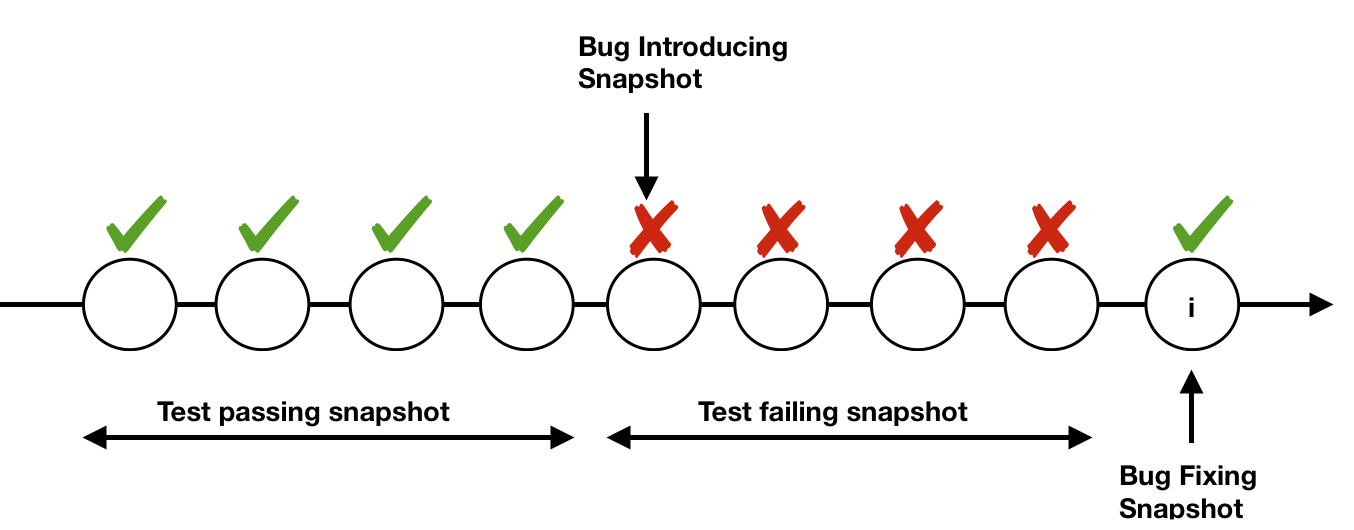
\includegraphics[width=\columnwidth]{img/snapshot1.png}
\caption{El Bug Introducing Snapshot es el \BIC}
\label{fig:snapshot1}       % Give a unique label
\end{figure}

La Figura~\ref{fig:snapshot2} muestra c\'omo se aplica la prueba hipot\'etica cuando existe un \BIC pero la prueba \TSB no se puede ejecutar despu\'es de una instant\'anea. Esto se debe a que la funci\'on o caracter\'istica probada no se encuentra presente en ese momento. En este caso, el primer \BIS identificado es el \BIC porque cuando introdujo la funci\'on o caracter\'istica probada, \'esta conten\'ia errores.

\begin{figure}[ht]
\centering
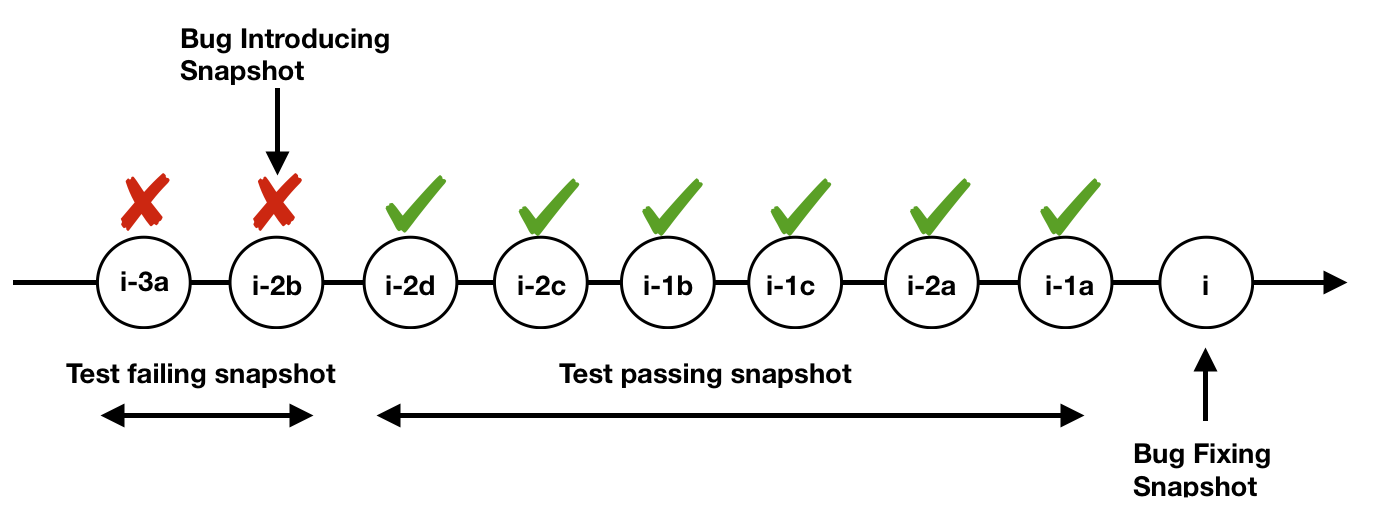
\includegraphics[width=\columnwidth]{img/snapshot2.png}
\caption{El Bug Introducing Snapshot es el \BIC }
\label{fig:snapshot2}       % Give a unique label
\end{figure}

La figura~\ref{fig:snapshot3} muestra c\'omo se aplica la prueba hipot\'etica cuando no hay \BIC y el \TSB se puede ejecutar indefinidamente a lo largo del historial del c\'odigo fuente. La \TSB siempre falla con el entorno \BFS en las instant\'aneas, pero si se establece el entorno anterior, pasar\'a en la instant\'anea descendente. Por lo tanto, el primer \BIS antes de \BFC ser\'a el \FFC, no existe \BIC en el conjunto de commits antecesores.

\begin{figure}[ht]
\centering
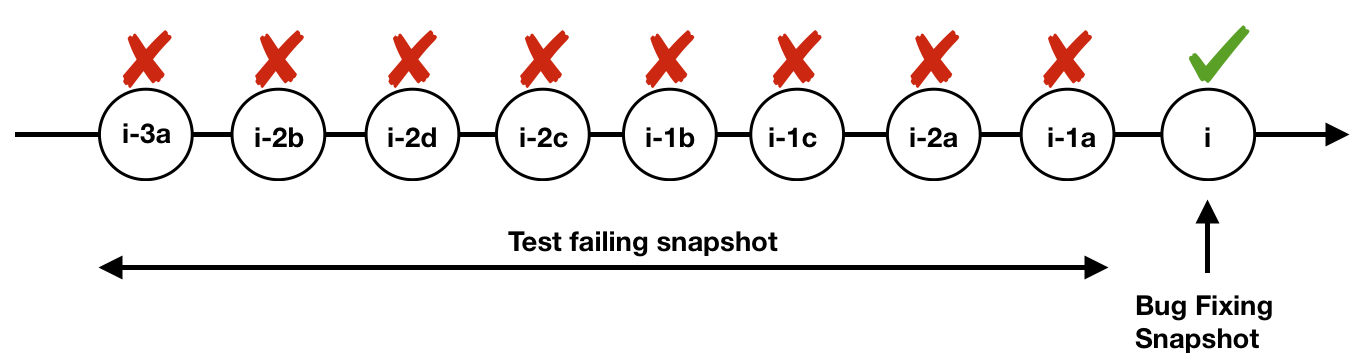
\includegraphics[width=\columnwidth]{img/snapshot3.png}
\caption{El Bug Introducing Snapshot es el \FFC }
\label{fig:snapshot3}       % Give a unique label
\end{figure}


\subsection{Criterio para aplicar el \TSB}

Cuando la historia de un proyecto es lineal, los investigadores pueden usar uno por uno todo el conjunto de commits pertenecientes al \ACSet{i} para ejecutar el \TSB en la rama master. Pero cuando la historia del proyecto no es lineal si no que puede tener m\'ultiples ramas, encontrar el \BIC o \FFC puede llegar complicarse. Esto se debe a que el error podr\'ia estar presente en algunas de las ramas existentes y ausente en otras, y el concepto de \FFC puede llegar a ser incierto. Sin embargo, a primera vista, y suponiendo que te\'oricamente la prueba se puede ejecutar para todas las instant\'aneas en el \ACSet{i}, los resultados del \TSB a\'un podr\'ian ser v\'alidos para identificar el \FFC o \BIC ya que todav\'ia encuentran secciones en una o m\'as ramas donde la prueba fallar\'ia. 

Es posible que, en algunos escenarios, el modelo propuesto defina el \BIC como el topol\'ogicamente primero en la secci\'on de m\'ultiples instant\'aneas con errores. Puede suceder que dos o m\'as commits en paralelo comienzan a fallar hasta llegar al \BFC, sin embargo, se puede considerar que esto es una indicaci\'on de que el error fue introducido en el c\'odigo fuente, independientemente, en varias ramas o fue copiado (o escrito id\'enticamente por casualidad) en varias ramas. Nuestra hip\'otesis es que estos escenarios no son comunes y por el momento podr\'iamos no centrarnos en ellos, pero al menos debemos mencionarlos en el modelo te\'orico.

Por lo tanto, para definir estos casos, podr\'iamos extender la noci\'on de \BIC a ``el conjunto de \BIC, que ser\'ia ``los cambios correspondientes a la primera instant\'anea que falla, continuamente hasta llegar al \BFC, en varias ramas que conducen hasta el \BFC''.

Adem\'as, los investigadores pueden decir el tipo de \BIS en base a si es un \BIC, un \FFC, ambos, o indecisos.

 \begin{enumerate}
	\item \textbf{Indeciso}:  Cuando no podemos encontrar el \FFC o el \BIC. En esta situaci\'on, no podemos estar seguros de encontrar el \FFC entre todos los commits pertenecientes al conjunto \ACSet{b} usando el \TSB 
	\item \textbf{El \FFC es el \BIC}: Cuando podemos encontrar el \FFC entre todos los commits del conjunto \ACSet{b} usando la prueba \TSB y adem\'as podemos estar segurod de que ese commit es la causa del error porque introdujo las l\'ineas err\'oneas en el c\'odigo fuente.
	\item \textbf{solo es un \FFC}: Cuando el error no fue causado por un cambio perteneciente al conjunto \ACSet{b} si no que, un cambio en el entorno o un cambio en las dependencias del proyecto caus\'o el error y usando el \TSB podemos encontrar la primera instant\'anea que manifiesta el error.
 \end{enumerate}
 
Automatizar este proceso es tedioso y complejo, debido a la necesidad de recrear todas las dependencias externas utilizadas en el proyecto en cada una de las instant\'aneas previas a un \BFC. Sin embargo, seguimos confiando en que la automatizaci\'on puede ser posible en base a declaraciones de estudios anteriores como el realizado por Bowes~\emph{et al.}. Este estudio proporciona una lista b\'asica de principios de prueba que se centra en diferentes aspectos de calidad, adem\'as de la efectividad o la cobertura. Para nuestra investigaci\'on, el principio m\'as interesante es la (in)dependencia de prueba que describe que una prueba debe poder ejecutarse en cualquier orden y de forma aislada. La prueba no debe depender de otras pruebas de todos modos, para permitir a los profesionales agregar nuevas pruebas sin tener en cuenta las dependencias o los efectos que puedan tener en las pruebas existentes~\cite{bowes2017good}.

\section{Objetivos y Problema}
El objetivo principal de esta tesis es desarrollar un modelo te\'orico que ayude a identificar inequ\'ivocamente el cambio que introdujo la l\'inea o l\'ineas err\'oneas en el c\'odigo fuente de un programa, a partir del arreglo del error. Para ello, esta tesis realiza un an\'alisis minucioso sobre las t\'ecnicas actuales usadas para identificar la causa del error, detallando el problema actual que impide que estas t\'ecnicas identifiquen correctamente el cambio en el que el error fue introducido en el c\'odigo fuente. En concreto, esta tesis cuantifica las limitaciones encontradas en el algoritmo SZZ. Desde hace mas de diez a\~nos, este algoritmo es el m\'as utilizado para encontrar el origen del error a pesar de que tanto investigadores como desarrolladores y profesionales son conscientes de sus limitaciones. La falta de otro modelo que explique como encontrar el verdadero origen de un error, as\'i como la falta de definici\'on de lo que significa un fallo, causan que todos los estudios que analizan el momento en el que un error es introducido empiecen con la misma premisa ``Las l\'ineas modificadas que arreglaron el error son potencialmente culpables de introducir el fallo en el sistema''. Esta premisa trata a los errores como una variables est\'aticas que permanece en el sistema desde que se introducen, cuando en realidad los errores no deben ser estudiados como variables est\'aticas, ya que factores externos como cambios el las APIs o la evoluci\'on interna del sistema causan que una l\'inea correcta en un un momento determinado empiece a manifestar el error en un momento posterior.   

Para resolver la falta de definiciones y las limitaciones yacentes en los algoritmos actuales. Esta tesis propone un modelo te\'orico para definir qu\'e cambios introducen errores en el c\'odigo fuente. Este modelo se basa en la suposici\'on que existe una prueba de test perfecta que puede ejecutarse indefinidamente en toda la historia del proyecto con el fin de descubrir cu\'ando se insert\'o el error en el c\'odigo fuente del proyecto. Adem\'as, este modelo puede usarse como marco para validar los resultados obtenidos en otrros enfoques. Establecer este marco es uno de los principales valores de la tesis porque la literatura previa ha podido calcular con exactitud la precisi\'on y el recall ``real'' de los algoritmos actuales usados para identificar el \BIC.

A continuaci\'on se puede encontrar un listado de las contribuciones principales de la tesis:
\begin{enumerate}
  \item{Revisi\'on de la literatura asistem�tica en el uso del algoritmo SZZ:}
  	\begin{enumerate}
		\item{Una visi\'on general del impacto que el algoritmo SZZ ha tenido hasta ahora en el \'area de ESE.}
		\item{Una visi\'on general de c\'omo los estudios que usan el algoritmo SZZ abordan la reproducibilidad en su trabajo de investigaci\'on.}
		\item{Un an\'alisis de c\'omo estos estudios manejan las limitaciones del algoritmo SZZ}
	\end{enumerate}
  \item{Un modelo te\'orico para identificar inequ\'ivocamente los cambios de introducci\'on de errores}
  	\begin{enumerate}
		\item{Una definici\'on detallada del Bug-Introducing Change y First-Failing Change}
		\item{El criterio usado para aplicar el modelo.}
	\end{enumerate}
  \item{Estudio emp\'irico sobre la aplicaci\'on del modelo propuesto}
  	\begin{enumerate}
		\item{La frecuencia de \BFC inducida por \BIC en Nova y ElasticSearch}
		\item{El conjunto de datos ``est\'andar de oro''}
	\end{enumerate}
  \item{Cuantificaci\'on del algoritmo SZZ.}
\end{enumerate}

\section{Metodolog\'ia}
La metodolog\'ia utilizada en este estudio emp\'irico se divide en dos partes, la primera parte es la etapa de filtrado donde los investigadores se aseguran que los conjuntos de datos extra\'idos de Nova y ElasticSearch cumplen con los requisitos para ser analizados usando la teor\'ia de la introducci\'on de errores descrita anteriormente. La segunda etapa describe cada uno de los pasos que hay que seguir desde que se selecciona un \BFC hasta que se identifica el \BIC y el \FFC.

La figura~\ref{fig:diagrama} proporciona una visi\'on general de cada paso involucrado en nuestro estudio, as\'i como los resultados que se obtendr\'ian.


\begin{figure}[ht]
\centering
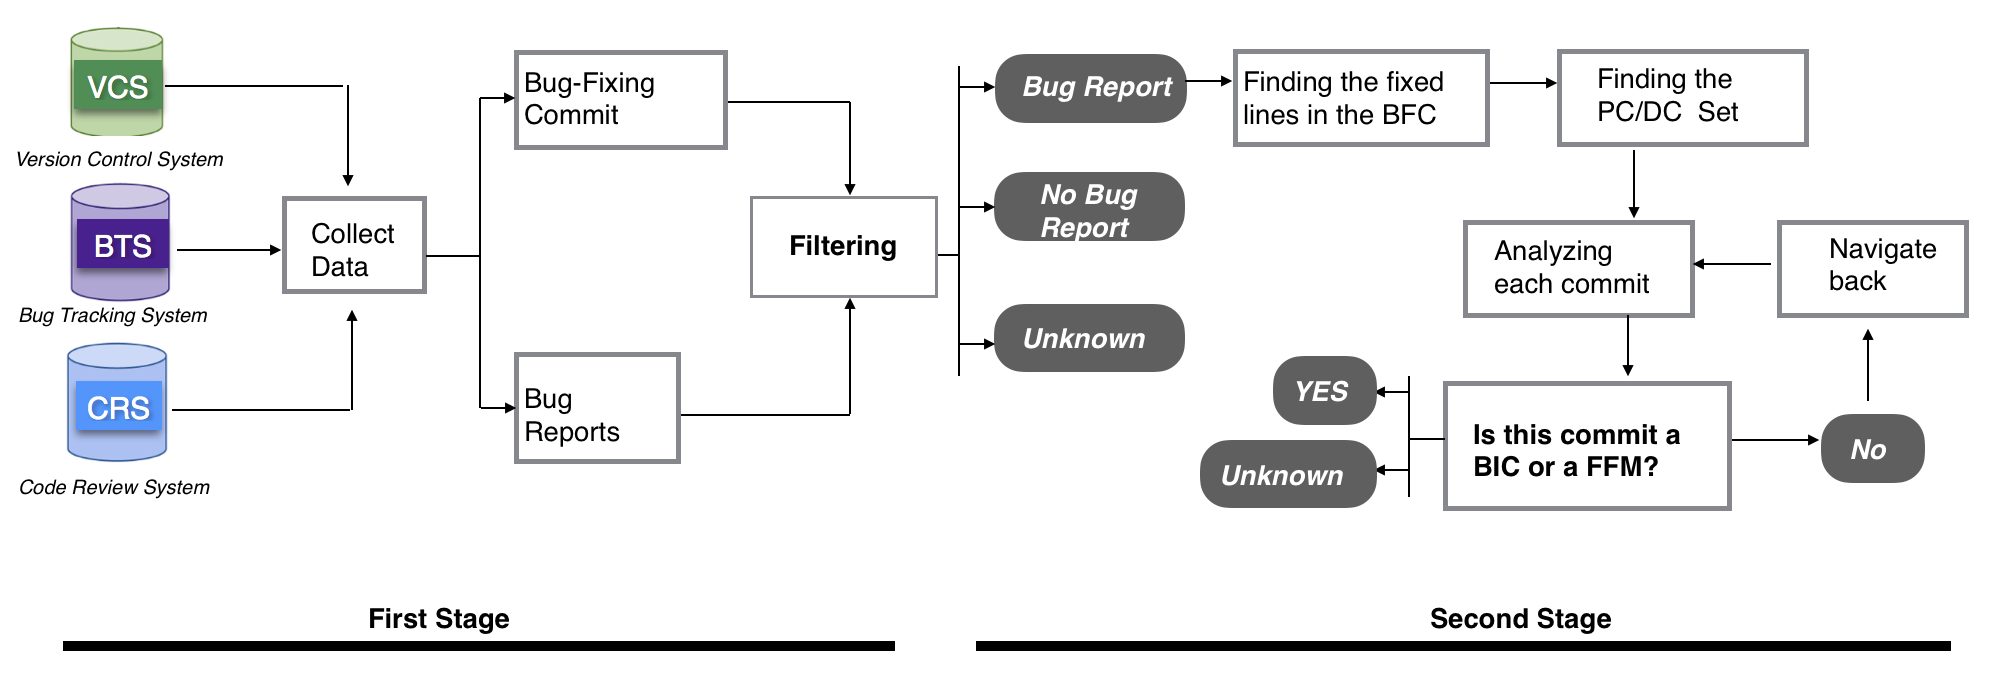
\includegraphics[width=\columnwidth]{img/diagram.png}
\caption{Descripci\'on de los pasos involucrados en nuestro an\'alisis }
\label{fig:diagrama}       % Give a unique label
\end{figure}


\subsection{Primera Etapa: Filtrado}
\label{sec:methodologyFS}

Esta etapa garantiza que el modelo propuesto se pueda aplicar a los informes de errores extra\'idos anteriormente. Uno de los requerimientos necesarios en esta etapa es que los informes de error que pasen a la siguiente etapa describan realmente errores, y a pesar de la estricta pol\'itica de etiquetado de errores presente en ElasticSearch y la clasificaci\'on manual para distinguir informes de errores de otro tipo de errores llevada acabo en Nova, esta etapa se encarga de analizar cuidadosamente cada informaci\'on en los informes de errores para garantizar que el ``est�ndar de oro'' obtenido al final del estudio es lo m\'as preciso posible. Consecuentemente, el conjunto de datos tanto en Nova como en ElasticSearch, solo debe almacenar errores que se consideran errores en el momento de su correci\'on. Por ejemplo, hay una prueba (hipot\'etica) que falla justo antes del \BFC pero no falla inmediatamente despu\'es. Esto asegura que si existen problemas que se describen como errores pero se descubre que son nuevas peticiones para a\~nadir nuevas caracter\'isticas o sugerencias de mejoras, ser\'an excluidas.

\subsection{Segunda etapa: identificar el \BIC y el \FFC}
\label{sec:methodologySS}

Esta etapa tiene como entrada un conjunto de informes de errores de Nova y ElasticSearch que describen errores reales en el momento de su correcci\'on. En esta etapa se require identificar manualmente el \BIC y el \FFC correspondiente a un \BFC dado, aunque en algunas ocasiones, no se puede identificar ning\'un \BIC como el inductor del \BFC.  La identificaci\'on de un \BIC dado un \BFC significa que el error estaba presente en el momento de escribir las l\'ineas en el c\'odigo fuente. El \BIC puede estar en el commit previo o en cualquiera de los commits descendientes o antecesores, por tanto se requiere analizar manualmente cada uno de ellos para garantizar la credibilidad en el ``est\'andar de oro''. En los casos en que el error no est\'a presente en el momento de insertar las l\'ineas en el c\'odigo fuente, significa que no podemos identificar ning\'un \BIC y es necesario encontrar el \FFC. Para entender mejor este proceso, los pasos seguidos se detallan a continuaci\'on donde se hace uso de la terminolog\'ia que se encuentra descrita en la secci\'on 5.1.1.

%Requirements have changed invalidating previous assumptions (GDPR). In this case there is no Bug-Introducing Commit.
%External resources have been modified (GitHub API). In this case there is no Bug-Introducing Commit.
%Internal resources have been modified (directory structure and permissions; the Chromium bug). In this case there is a Bug-Introducing Commit but this commit did not directly affect the lines of code modified in the Bug-Fixing Commit, so SZZ cannot find it; this Bug-Introducing Commit would have taken place after the previous commit and before bug reporting. 

\subsubsection{Encontrar las l\'ineas que corrigieron el error}

En esta etapa, se debe identificar las l\'ineas de c\'odigo fuente que corrigi\'o el error; nos referimos a un error gen\'erico como $b$. Es importante:
\begin{itemize}
	\item Identificar los commits que corrigieron el error entre el conjunto \setBFC{b}. En la mayor\'ia de los casos analizados, este conjunto siempre fue unitario, lo que significa que para cada error hab\'ia un \BFC \'unico que lo arreglaba. Sin embargo, encontramos algunas excepciones, por ejemplo, el informe de error \#1442795\footnote{\url{https://bugs.launchpad.net/nova/+bug/1442795}} ten\'ia dos \BFC diferentes que corrigieron el error. 
	Para simplificar este proceso, la metodolog\'ia asume que el conjunto \setBFC{b} es unitario, y en el caso donde m\'as de un \BFC corrigi\'o el error, la metodolog\'ia analizar\'a ambos commits indistintamente para identificar el \BIC.
	\item Encuentra las l\'ineas que fueron modificadas por el \setBFC{b} para corregir el error, nos referiremos al conjunto de l\'ineas a\~nandias, modificadas y eliminadas por un commit como \LC{c} donde $c$ es el \BFC:
El \BFC se encuentra vinculado a un informe de error, en este informe se encuentra disponible toda la informaci\'on relacionada con el proceso de revisi\'on del c\'odigo. Aplicando la herramienta \textit{``git diff ''} es posible identificar qu\'e l\'ineas se han agregado, modificado o eliminado entre la versi\'on despu\'es del \BFC y la anterior. Tambi\'en existe la posibilidad de visualizar los cambios realizados por el \BFC usando la herramienta web de GitHub donde visualmente se observan de una forma muy intuitiva los cambios realizados en el \BFC.
	\item Filtrar las l\'ineas modificadas o eliminadas que no son c\'odigo fuente:
Algunas l\'ineas que se han modificado o eliminado pueden no contienen c\'odigo fuente (por ejemplo, comentarios o l\'ineas en blanco). \'Estas l\'ineas no se consideran en el posterior an\'alis. Adem\'as, como caso excepcional, en el conjunto de \BFC analizados se encontraba un \BFC\footnote{\url{https://github.com/elastic/elasticsearch/commit/beaa9153a629c0950182e4e8c4f8eedd1c63f49f}} que arregl\'o dos informes de errores diferentes al mismo tiempo. En este caso, se eliminaron el conjunto de \LC{c} relacionadas con el informe de error que no se estaba analizando.
\end{itemize}.

\subsubsection{Determinar qu\'e commit cambi\'o por \'ultima vez cada una de las l\'ineas \LC{c}.}

Cada una de las l\'ineas modificadas por un \BFC tiene un \'unico commit previo. Sin embargo, podr\'ia haber tantos commits previos como l\'ineas modificadas en por un \BFC, (la figura del \'arbol geneal\'ogico representado en la subsecci\'on 5.1.2 muestra visualmente este concepto). Consecuentemente,  el resultado obtenido en este paso es un conjunto de todos los commits previos del error $b$, \PC{b}.

\subsubsection{Analizando cada una de los commits previos, y sus commits descendientes, para identificar el \BIC y el \FFC}

En este paso se utiliza la informaci\'on disponible en la descripci\'on del ticket, en los registros del \BFC y en commits pertenecientes al conjunto de \PC{b} para analizar si existe o no un \BIC y si manualmente podemos identificarlo. Despu\'es de entender el error y los cambios que arreglaron ese error, es necesario identificar el \BIC en caso de que exista, as\'i como el \FFC. Consecuentemente, la identificaci\'on del \BIC comienza con el an\'alisis del conjunto de \PC{b}, para cada uno de los commits pertenecientes al conjunto de \PC{b} se analizan las l\'ineas modificadas para encontrar si alguno de los commits previos introdujo el error. En este punto, hay tres escenarios diferentes y el comportamiento es difiere seg\'un las siguientes condiciones:

\begin {enumerate}
	\item \textit {El commit insert\'o las l\'ineas que contienen el error}: Este commit es el \BIC porque insert\'o las l\'ineas defectuosas en el c\'odigo fuente en el momento de su escritura. El \BIC que a su vez es el \FFC se pudo identificar porque es el primer commit que manifest\'o el comportamiento incorrecto. De acuerdo con el modelo te\'orico, el TSB ejecutado en el \BFC pasa y el \BIS es una de las instant\'aneas previas, es decir, es uno de los commits previos del \BFC.
	\item \textit {El commit no inserta las l\'ineas que contienen el error}: en este caso, hay dos resultados posibles:
	\begin {itemize}
		\item Las l\'ineas del commit son correctas ya que no insertaron el error en las l\'ineas del c\'odigo fuente en el momento de su escritura y otros factores externos causaron que esas l\'ineas se volvieran defectuosas. En este escenario, no hay un \BIC en  y el an\'alisis debe centrarse en comprender si este commit es el \FFC. De acuerdo con el modelo te\'orico, la TSB se ejecuta en todo el \ACSet{b} y pasa en el \BFC pero siempre falla en las instant\'aneas de los ancestros. Sin embargo, si se cambia el entorno, el TSB falla en el \BFC pero pasa en la instant\'aneas anteriores, y el primer \BIS que falla en la secuencia continua de \BIS es el \FFC.
		\item Las l\'ineas del commit son cambios sint\'actico y modificaciones sem\'anticas equivalentes (refactorizaciones): Esto significa que el commit conserva el mismo comportamiento que antes, por lo tanto, es necesario volver a navegar, en el conjunto de \DCSet{b} y volver al primer punto de esta lista para identificar el \BIC.
	\end{itemize}
	\item \textit {No es seguro que el commit insertase el error}: en este escenario, es importante continuar navegando por el conjunto de \DCSet{b}, si el commit insert\'o por primera vez en las l\'ineas descendentes al conjunto de lineas del \LC{c} y no podemos estrar seguros de que esas l\''ineas contengan el error, el commit se clasifica como ``indecisa''. Esto significa que despu\'es del an\'alisis, el \BIC no se pudo encontrar manualmente a pesar de que podemos asegurar su existencia, o que no podemos asegurar el \FFC o \BIC debido a la falta de informaci\'on.
\end{enumerate}

\subsection{Resultados de las etapas}

Al final del proceso, hay tres resultados posibles para cada informe de error analizado. Los resultados se basan en la identificaci\'on inequ\'ivoca del \BIC y del \FFC dado un \BFC.
Estos resultados se encuentran explicados a continuaci\'on:
 
 \begin{itemize}
	\item Un \BFC fue inducido por un \BIC: en este caso es seguro que al menos hay un commit que introdujo las l\'inea(s) err\'onea(s) entre el conjunto de commits previos, o conjunto de commits descendientes o el conjunto de commits de ancestros. Sin embargo, durante el an\'alisis manual puede ocurrir que:
	\begin{enumerate}
		\item El momento se pudo identificar manualmente o,
		\item El momento no se pudo identificar manualmente.
	\end{enumerate}
	Adem\'as, en este escenario, el \BIC es tambi\'en el \FFC.
	\item Un \BFC no fue inducido un \BIC: en este caso es seguro que ninguna l\'inea insertada en el c\'odigo fuente conten\'ia el error cuando se introdujo el commit, y otros factores como por ejemplo, los cambios en las necesidades internas del proyecto, o cambios en los recursos externos consumidos por el proyecto, provocan que el c\'odigo se vuelva defectuoso. Tambi\'en se puede confirmar que ninguno de los commits antecesores insert\'o las l\'ineas incorrectas, por lo que no se puede culpar a ninguno de ellos como el \BIC y solo se podr\'a identificar la primera vez que manifiesta el error en el c\'odigo. Adem\'as, en este escenario puede ocurrir que:
	\begin {enumerate}
		\item El momento se pudo identificar manualmente o,
		\item El momento no se pudo identificar manualmente. 
	\end {enumerate}
	\item No est\'a si un \BFC due inducido por un \BIC: algunos informes de errores no detallan suficiente informaci\'on sobre el error y el \BFC no es suficiente para decidir si hay o no un \BIC. Adem\'as, algunos commits son muy complejos para comprender sus cambios y no se puede decidir si insertaron o no el error.
\end{itemize}

 
\section{Resultados}

Hay tres secciones diferentes para discutir los resultados obtenidos en el Cap\'itulo 4, Cap\'itulo 5 y Cap\'itulo 6.

\subsection{Reproducibilidad y credibilidad del algoritmo SZZ  }
\label{subsec:resultadosSLR}

En el Cap\'itulo 4 de esta tesis se detalla el estudio de la revisi\'on sistem\'atica de la literatura (\emph{SLR}) sobre el uso del algoritmo SZZ en estudios emp\'iricos de ingenier\'ia del software (\emph{ESE}).La SLR demost\'o que el algoritmo es ampliamente usado en la ESE y que posee una alta relevancia, no se limita solamente a una audiencia espec\'ifica, si no que se ha difundido por numerosas publicaciones en revistas y conferencias importantes en varias areas de la Ingenier\'ia del Software. 
Tabla~\ref{tablaMedia} muestra los diferentes medios de publicaci\'ion que han usado el algoritmo SZZ. Hay cuatro diferentes medios: Tesis universitarias, art\'iculos en workshops, art\'iculos en conferencias y symposiums, y art\'iculos en revistas.


%\alex{Refer to core rankings to justify why you believe MSR, ICSE, ICSME etc to be good conferences. At the same time you can argue.... the impact of SZZ is limited to people conducting empirical studies....... }\gema{Almost done}
\begin{table}
% increase table row spacing, adjust to taste
\renewcommand{\arraystretch}{0.8}
% if using array.sty, it might be a good idea to tweak the value of
%\extrarowheight as needed to properly center the text within the cells
\caption{ Los tipos o publicaciones m\'as frecuentes que utilizan completamente el algoritmo SZZ (N = 187). \emph{\#diferentes} cuenta los diferentes lugares en cada grupo, \emph{\#publications} cuenta el n\'umero total de publicaciones en ese tipo de lugares.}
\label{tablaMedia}
\centering
% Some packages, such as MDW tools, offer better commands for making tables
%% than the plain LaTeX2e tabular which is used here.
\begin{adjustbox}{max width=\textwidth}
\begin{tabular}{|l|r|r|}
\hline
Tipo & \# Diferentes & \# publicaciones  \\
\hline
\hline
 Revistas & 21 & 42\\
\hline
 Conferencias \& Simposiums & 40 & 102\\
\hline
Workshops & 13 & 13\\
\hline
Tesis universitarias & 20 & 30 \\
\hline
\end{tabular}
\end{adjustbox}
\end{table}

Durante la SLR se ha observado que las limitaciones del algoritmo SZZ son bien conocidas y documentadas. Se han propuesto mejoras para mitigar las limitaciones que presenta, pero hasta el moment no han llegado a tener demasiado \'exito. Adem\'as, mientras que las limitaciones de la primera parte del algoritmo, relacionadas con enlazar los Bug-Fixing Commits (\BFC) con lo bug reports, han obtenido significantes mejoras. Las propuestas para mitigar las limitaciones de la segunda parte, relacionadas con encontrar el Bug-Introducing Commit (\BIC), todav\'ia tiene espacio para mejorar.   

La SLR ha demostrado que la mayor\'ia de las publicaciones que usan el algoritmo SZZ, o sus versiones mejoradas: SZZ-1~\cite{kim2006automatic} y SZZ-2~\cite{williams2008szz}, no mencionan las limitaciones, y lo que resulta mas interesante es que las limitaciones de la primera parte del algoritmo resultan ser m\'as discutidas que las de la segunda parte a pesar de ser menos relevantes para la veracidad de los resultados obtenidos. La Tabla~\ref{tableSZZmejorado} muestra cu\'antas publicaciones han utilizado mejoras en el algoritmo SZZ para mitigar las limitaciones del original. Tenga en cuenta que la columna ``Mixed '' de la Tabla~\ref{tableSZZmejorado} se refiere a los documentos que han utilizado la versi\'on original, y alguna de las versiones mejoradas en el mismo estudio. En la Tabla~\ref{tableSZZmejorado} se puede observar que solamente el 38\% de las publicaciones analizadas usan la versi\'on \emph{original} SZZ.  Por tanto, para aumentar la reproducibilidad y credibilidad de los resultados, recomendamos que los investigadores que desarrollen modificaciones del algoritmo SZZ, publiquen el software implementado en sitios como \texttt{GitHub}, de este modo otros investigadores pueden \emph{fork} el proyecto. Esos \emph{forks} pueden ser f\'acilmente trazados, y los autores pueden preguntar por una espec\'ifica citaci\'on a su soluci\'on si otros autores hacen uso de ella. Adem\'as otra de las ventajas que posee el publicar el software implementado es que la reproducibilidad es m\'as espec\'ifica, debido a que en ocasiones los autores por falta de espacio no mencionan como funciona o como se implant\'o el algoritmo que han usado y es posible que este hecho esconda errores al reproducir el estudio.

\begin{table}[!t]
% increase table row spacing, adjust to taste
\renewcommand{\arraystretch}{0.8}
\begin{minipage}{\textwidth} 

% if using array.sty, it might be a good idea to tweak the value of
%\extrarowheight as needed to properly center the text within the cells
\caption{N\'umero de art\'iculos que han utilizado el algoritmo SZZ original, las versiones mejoradas del SZZ o algunas adaptaciones para mitigar las amenazas de validaci\'on.}
\label{tableSZZmejorado}
\centering
% Some packages, such as MDW tools, offer better commands for making tables
%% than the plain LaTeX2e tabular which is used here.
\begin{tabular}{|c|c|c|c|c|}
\hline
  & Original SZZ only & SZZ-mejorado only & SZZ-modificado & Mezcla  \\
\hline
\hline
\# art\'iculos &  71 (38\%) & 26 (14\%)~\footnote{22 (12\%) de los art\'iculos usan el SZZ-1 y solo 4 (2\%) de los art\'iculos usan el SZZ-2.} &  75 (40\%)  & 15 (8\%) \\
\hline
\end{tabular}
\end{minipage}
\end{table}

Hemos encontrado que la reproducibilidad de las publicaciones es limitada, y los paquetes de r\'eplica se ofrecen muy raramente.  La Tabla~\ref{tableReplica} ofrece el n\'umero de estudios que a)contiene un paquete de reproducci\'on, b) han detallado cuidadosamente la metodolog\'ia para permitir las reproducciones de sus estudios. Hemos clasificado las publicaciones en cuatro grupos: i) publicaciones que ofrecen un paquete de reproducci\'on (\emph{paquete}), ii) publicaciones que detallan la metodolog\'ia y los datos utilizados (\emph{Environment}), iii) publicaciones que tienen ambos \emph{Ambos}) y iv) Ninguno (\emph{Ninguno}).

De las 187 publicaciones, 43 ofrecen un paquete de reproducci\'on y 96 cuidadosamente detallan los pasos seguidos y los datos utilizados. Adem\'as, solo 24 de los art\'iculos proporcionan tanto el paquete de replicaci�n como la metodolog�a y los datos detallados. 72 de los documentos no ofrecen un paquete de reproducci\'on o una descripci\'on detallada de la metodolog\'ia y los datos usados. 

\begin{table}[!t]
% increase table row spacing, adjust to taste
\renewcommand{\arraystretch}{0.8}
% if using array.sty, it might be a good idea to tweak the value of
%\extrarowheight as needed to properly center the text within the cells
\caption{Publicaciones por su reproducibilidad: Filas: \emph{Si} significa el n\'umero de trabajos que cumplen cada columna, mientras que su complemento es \emph{No}. Columnas: \emph{Paquete} es cuando ofrecen un paquete de reproducci\'on, \emph{Environment} cuando proporcionan la metodolog\'ia detallada y un conjunto de datos usados. Tenga en cuenta que \emph{Both} es la intersecci\'on de \emph{Paquete} y \emph{Environment}. (N = 187)}
\label{tableReplica}
\centering
% Some packages, such as MDW tools, offer better commands for making tables
%% than the plain LaTeX2e tabular which is used here.
\begin{tabular}{|c|c|c|c|c|}
\hline
    & Solo paquete  & Solo Environment  & Ambos & Ninguno \\
\hline
\hline
Si & 19 & 72 & 24 & 72 \\
\hline
No & 168 & 96 & 163 & 115 \\
\hline
\end{tabular}
\end{table}

A pesar de que usar las versiones mejoradas del algoritmo SZZ ayuda a aumentar la precisi\'on del algoritmo como se\~nala~\cite{rahman2012clones}: ``Accuracy in identifying  Bug-Introducing Commit may be increased by using advanced algorithms (Kim et al. 2006, 2008)'', raramente se usan -- s\'ole el 22\% de las publicaciones usan una de las dos mejoras propuestas para el algoritmo SZZ. Parece que los investigadores prefieren reinventar la rueda, el 49\% de los art\'iculos analizados usan una versi\'on modificada o ``ad-hoc'' por ellos mismos del SZZ, en vez de utilizar las mejoras propuestas en otros art\'iculos. Una posible raz\'on para explicar este comportamiento poor\'ia ser que los art\'iculos que describen el SZZ o cualquiera de sus mejoras propuestas, SZZ-1 y SZZ-2, no aportan el c\'odigo software de la implementaci\'on. Por ello, los investigadores tienen que implementar el software desde cero para poder usarlo en sus investigaciones. Nuestros resultados muestran que en dicha situaci\'on, lo que se hacer es usar el concepto general que describe el algoritmo SZZ y a\~nadir algunas modificaciones con el prop\'osito de mitigar algunas de las limitaciones presentes en el SZZ original. Para todos las soluciones identificadas como ``ad-hoc'', no se ha encontrado ninguna raz\'on que explique el por qu\'e no se implementaron las otras mejoras del  SZZ. Otro problema importante es el etiquetado del las mejores de SZZ, ya que no han sido ni etiquetadas ni enumeradas. Cuando una versi\'on mejorada del SZZ es usada en los art\'iculos, a menudo lo autores se refieren a ella como SZZ, dificultando el seguimiento, la reprodureproci\'on y la r\'aplica de sus resultados.

Por otro lado, en esta tesis se ofrece una simple manera de medir la facilidad de reproducci\'on y credibilidad en los art\'iculos de investigaci\'on. Esta medida se basa en puntuar cinco caracter\'isticas que se analizaron en los art\'iculos. Si las preguntas fueron respondidas positivamente, el art\'iculo fue marcado con un puntaje positivo, de lo contrario con un 0:
 
\begin{enumerate}
\item �El estudio informa de las limitaciones del SZZ? (puntaje = 1 punto)
� \item �Los autores llevan a cabo una inspecci\'on manual de sus resultados? (puntaje = 1 punto)
� \item �El estudio aporta un paquete de reproducibilidad? (puntaje = 2 puntos)
� \item �El estudio proporciona una descripci\'on detallada de los m\'etodos y datos utilizados? (puntaje = 1 punto)
� \item �Utiliza el estudio una versi\'on mejorada de SZZ? (puntaje = 2 puntos)
\end{enumerate}

Los art\'iculos que sumen puntos del  0 al 1 se consideran \emph{Pobres} de ser reproducibles y poseer resultados cre\'ibles. Los art\'iculos que sumen puntos del 2 al 4 se consideran \emph{Justos} de ser reproducibles y poseer resultados cre\'ibles. Aquellos art\'iculos que sumen puntos del  5 al 6 se consideran \emph{Buenos} de ser reproducibles y poseer resultados cre\'ibles. Finalmente los art\'iculos que sumen 7 puntos  se consideran \emph{Excelentes} de ser reproducibles y poseer resultados cre\'ibles

%A pesar de que esta medida ha sido creada para los estudios que utilizan el algoritmo SZZ, pensamos que puede ser f\'acilmente adaptada a otros art\'iculos de investigaci\'on en ESE. As\'i, los autores pueden f\'acilmente evaluar si sus art\'iculos son reproducibles y ofrecen resultados confiables (por ejemplo, cuando la puntuaci\'on obtenida es igual a 5 o superior). Aunque a menudo nos dirigimos a los autores directamente, no debemos olvidar que los revisores ejercen una responsabilidad importante en el proceso cient\'ifico. Hemos visto que los autores a menudo son detallistas al presentar sus investigaciones, pero los revisores deben tener la visi\'on requerida para evaluar los estudios teniendo en cuenta esos detalles, y ayudando a los autores a aumentar el nivel de sus investigaciones. Por tanto, recomendamos a los revisores preguntarse estas preguntas, adaptadas al contexto de la investigaci\'on, cuando lleven a cabo revisiones de art\'iculos que usen heur\'sticos y asunciones. 

Durante el an\'alisis tambi\'en hemos observado que raramente se encuentran informes exhaustivos completos de la reproducibilidad, solamente se han clasificado un 15\% de los art\'iculos como \emph{buena y excelente calidad con respecto a la reproducibilidad}. La comunidad de  investigaci\'on debe poner mayor atenci\'on a estos aspectos; nosotros creemos que se est\'a otorgando demasiada atenci\'on a los resultados finales (el \emph{producto} de la investigaci\'on: nuevo conocimiento) en comparaci\'on con el proceso de investigaci\'on. Como investigadores en el campo de la ingenier\'ia del software sabemos que ambas partes -- una alta calidad del producto y una alta calidad del proceso -- son esenciales para obtener progresos exitosos a lo largo del tiempo~\cite{kan2002metrics}.

Para resumir, consideramos importante resaltar algunas de las lecciones aprendidas despu\'es de llevar a cabo la SLR. El algoritmo SZZ est\'a basado en heur\'isticos y asunciones, por tanto para aportar unos resultados m\'as cre\'ibles, recomendamos que los investigadores especifiquen y argumenten el uso de esos m\'etodos y algoritmos cuyo fin es mitigar las limitaciones presentes en el SZZ en sus estudios. Ser consciente del riesgo de cada asunci\'on usada y si es necesario, validar manualmente una porci\'on de los resultados obtenidos. Adem\'as, para llevar a cabo estudios emp\'iricos, los autores deben ser conscientes que para permitir la reproducci\'on de sus publicaciones, el mejor m\'etodo es incluir un paquete de reproducci\'on que puede estar p\'ublicamente disponible junto con su publicaci\'on (idealmente para siempre). Por otro lado, ellos tambi\'en tiene que ser conscientes de que algunas caracter\'isticas en sus estudios pueden cambiar, por ejemplo los entornos del software, causando que programa y los datos se encuentren obsoletos, por lo que es necesario detallar y describir con precisi\'on cada uno de los elementos, m\'todos y software usados durante el estudio.

\subsection{Teor\'ia de Inserci\'on del error}
\label{subsec:teoriaresultado}

Esta tesis propone una soluci\'on al problema actual de identificar el  Bug-Introducing Commit (\BIC) dado un commit que arregla un error (\BFC). Actualmente, la mayor parte del trabajo se basa en m\'etodos y t\'ecnicas formuladas bajo la suposici\'on intr\'insecamente err\'onea de que las l\'ineas de c\'odigo que se han modificado para corregir el error, son las l\'ineas que han introducido el error en primer lugar. La naturaleza problem\'atica de esta suposici\'on es conocida, como se ha demostrado anteriormente en la revisi\'on sistem\'atica de la literatura. Sin embargo, esta tesis hace una contribuci\'on importante al tratar de cuantificar el alcance del problema y al detallar un nuevo modelo de introducci\'on de errores para encontrar la primera vez que el software manifiesta un comportamiento incorrecto, sin la necesidad de culpar a un cambio como el  Bug-Introducing Commit, si no que identifica el primer cambio que establece el error y comprende ese momento en su contexto y dependencias.

Despu\'es de analizar varios informes de errores durante esta tesis, nos hemos dado cuenta que determinar d\'onde, cu\'ando y c\'omo se introdujo un error no es una tarea trivial, en la que a veces se involucran muchos investigadores con el fin de aclarar la naturaleza del error investigado. De hecho, no es f\'acil determinar si el error estaba presente en el c\'odigo en el momento de realizar un cambio. Por ejemplo, hay casos en los que las t\'ecnicas autom\'aticas actuales no pueden determinar el punto de introducci\'on del error, ya que no se puede identificar ning\'un commit previo. Uno de esos casos es cuando el commit/cambio que arregla el error (\BFC) solo introduce nuevas l\'ineas en el c\'odigo: en este caso, no hay forma de identificar el commit(s) previo(s) tal como lo definimos, ya que no hay ning\'u commit previo tocando las l\'ineas que han sido a\~nadidas. En este caso, solo la descripci\'on del informe del error o la descripci\'on y el c\'digo fuente del \BFC podr\'ia aclarar si las nuevas l\'ineas no se incluyeron debido a un olvido en un cambio ancestor o debido a que se incluyeron para satisfacer alg\'un nuevo requisito o nueva caracter\'istica del proyecto.

La SLR ayud\'o a cuantificar las limitaciones y los problemas que afectan a los algoritmos que se basan en el SZZ y son utilizados para identificar el Bug-Introducing Commit. Por tanto, teniendo esto en consideraci\'on, hemos propuesto un modelo en el que, por definici\'on, se integran todos los escenarios que imposibilitan el correcto funcionamiento del SZZ. El modelo propuesto es capaz de lidiar con estos escenarios y dar soluti\'on al problema. A continuaci\'on, explicamos brevemente como el modelo propuesto es capaz de abordar cada una de las limitaciones encontradas en la SLR. 	
\begin{enumerate}
	\item Identificaci\'on de m\'as de un commit previo: Nuestro modelo no trata de identificar los commits previos de las l\'ineas modificadas o eliminadas en un \BFC, si no que a trav\'es de un test comprueba el comportamiento de la funcionalidad que se arregl\'o en el \BFC en todas las instant\'aneas anteriores, descendientes y ancestrales del proyecto que esta siendo analizado hasta que encuentre la primera vez que el test falla.
	\item La utilizaci\'on de nuevas l\'ineas para corregir el error en el \BFC: Nuestro modelo no busca las l\'ineas que se han modificado o eliminado para corregir un error, sino que considera todos los cambios realizados en el \BFC, puesto que comprueba la funcionalidad que estaba fallando. Por tanto no distingue entre los \BFC que solo presentan l\'ineas a\~nadidas para descartarlos del an\'alsis.
	\item Presencia de cambios en el entorno o la configuraci\'on: Con nuestro modelo podemos detectar errores causados ??por un cambio en los entornos, ya sea que podr\'iamos ser capaces de reproducir el entorno anterior y posterior a un \BFC y observar que con un entorno espec\'ifico anterior al \BFC las pruebas de comprobaci\'on pasan en las instant\'aneas previas al \BFC, pero que con este entorno fallan en la instant\'anea del \BFC y al rev\'es. En este caso, habr\'a un \FFC pero no un \BIC.
	\item Varias modificaciones sobre una l\'inea: en nuestro modelo, no importa cu\'antas veces se haya modificado una l\'inea, ya que no se\~nala al \'ultimo cambio como el \BIC. La prueba de comprobaci\'on busca la primera vez que se inserta el error en la l\'inea que se est\'a probando.
	\item Nivel sem\'antico d\'ebil: como en el ejemplo anterior, el modelo propuesto trata con el inconveniente de tener un nivel sem\'antico d\'ebil porque no se centra en identificar el \'ultimo cambio, sino que prueba el comportamiento del c\'odigo.
	\item Un \BFC corrige a la vez m\'as de un error: en estos casos, nuestro modelo puede dise\~nar una prueba de comprobaci\'on espec\'ifica para cada error, buscando la primera vez que la prueba falla al comprobar la presencia de un error concreto en instant\'aneas anteriores al \BFC.
	\item Razones de compatibilidad:
	\item Errores latentes: el modelo identifica la primera vez que el error se insert\'o en el c\'odigo fuente utilizando el la prueba de comprobaci\'on, por tanto, no importa cu\'anto tiempo haya permanecido el c\'odigo defectuoso en el proyecto, porque te\'oricamente encontraremos la primera vez que se introdujo.   
\end{enumerate}

Muchos investigadores han basado sus m\'etodos para localizar el cambio que introdujo el error en el algoritmo SZZ o algoritmos similar, estos m\'etodos  carecen de medios para hacer frente a las limitaciones anteriormente comentadas, y por tanto tienen que formular algunas heur\'isticas que, por ejemplo, eliminan el \BFC con solo nuevas l\'ineas a\~nadidas porque no pueden rastrear esas l\'ineas, o eliminan commit numerosas modificaciones o eliminan los commits m\'as antiguos porque es poco probable que sean el \BIC ~\cite{da2016framework}. Como consecuencia, estos heur\'isticos pueden inducir a errores en los resultados, y mostrar un mayor porcentaje de precisi\'on del algoritmo al identificar el \BIC.

El SZZ es el algoritmo, hasta ahora, m\'as conocido y m\'as f\'acil de usar para identificar el cambio que introdujo el error o \BIC. Debido a esto, algunos estudios utilizan el algoritmo SZZ o variantes de \'el para extraer conjuntos de datos relacionados con el \BIC y los usan para alimentar sus modelos de predicci\'n o clasificaci\'n de errores. Por ejemplo, Ray \emph{et al.} usaron un conjunto de datos que se recopil\'o usando el algoritmo SZZ para estudiar la naturalidad del c\'odigo con errores \cite{rahman2014comparing}. Massacci \emph{et al. } evalu\'o la mayor\'ia de los modelos de detecci\'on de vulnerabilidades existentes en los navegadores web y us\'o muchos conjuntos de datos construidos usando el algoritmo SZZ \cite{massacci2014empirical}. Finalmente, Abreu \emph{et al.} us\'o el conjunto de datos obtenido en \cite{abreu2009practical} para estudiar c\'omo la frecuencia de comunicaci\'on entre desarrolladores afecta el hecho de introducir un error en el c\'odigo fuente.
%All in all, we believe in the benefit that this new concept to locate the \BIC and \FFC has in the Software engineering. In addition, with the classification of the origin of the bugs, we seed some more lights in the problem of emulating software faults realistically. However, to achieve greater bug location automation, we therefore need a concerted effort in testing to find ways or techniques to address the re-built problem and to build a test that can be automated or partially automated to find the FFC.

En general, este nuevo modelo propuesto, es capaz de distinguir entre dos momentos relevantes dado un commit que corrige un error \BFC, estos momentos son el momento de introducci\'on del error \BIC y el momento de manifestaci\'on de ese error en el c\'odigo \FFC. Mientras que el primer momento no siempre existe, debido a que algunos cambios externos o la evoluci\'on de los requisitos internos han cambiado provocando la falla, siempre hay un primer momento de fallo que indica cu\'ando el proyecto manifiesta el error corregido por el \BFC. Para obtener resultados cre\'ibles en las \'areas de predicci\'on de errores, categorizaci\'on de errores y los modelos de detecci\'on de errores, es necesario estudiar y distinguir estos dos momentos, ya que como demuestr\'o nuestro estudio emp\'irico los algoritmos o basados en el SZZ o variantes de \'el identifican desde el 26\% hasta el 38\% de falsos positivos ``reales''. Por lo tanto, estos resultados son alentadores para comenzar a pensar e implementar nuevos m\'etodos basados ??en el modelo te\'orico propuesto en esta tesis, o al menos, considerar reformular correctamente la definici\'on de insertar un error en el c\'odigo fuente. Ya que hasta ahora, el proceso de insertar un error en el c\'odigo ha sido considerado como un problema est\'atico, en el sentido que para los investigadores siempre ha estado presente el error que se ha corregido. Nuestra intuici\'on nos lleva a reclamar nuevos m\'etodos que sean capaces de distinguir entre l\'ineas defectuosas que contienen el error en el momento de insertarlas y l\'ineas limpias que no contienen el error en el momento de insertarlas. Esta disertaci\'on ha demostrado que existen otras razones externas e internas que provocan un fallo en el sistema, y no es justo culpar a un cambio anterior como el responsable de provocar el error cuando \'este cambio era correcto en el momento en el que introdujo, es decir, \'este cambio cumpl\'ia las funcionalidades, entornos, necesidades y requisitos del proyecto. Aunque hemos conseguido profundizar en el problema de identificar correctamente el cambio que provoc\'o el error, necesitamos dedicar m\'as esfuerzo para lograr una mayor automatizaci\'on del modelo propuesto, encontrar formas o t\'ecnicas que sean capaces de abordar tanto el problema de reconstrucci\'on de un entorno antiguo, como capaces de construir un test que pueda ser automatizado o parcialmente automatizado para encontrar los dos momentos m\'as importantes, el \BIC y el \FFC.	

\subsection{Estudio Emp\'irico: Aplicaci\'on de la teor\'ia propuesta para localizar el momento de introducci\'on de un error}

El estudio emp\'irico detallado en el Cap\'itulo 6 respalda la necesidad de b\'usqueda de un nuevo modelo para identificar inequ\'ivocamente los cambios que introducen errores, ya que no siempre es obvio identificar y entender c\'omo se introducen los errores en el c\'odigo fuente con los m\'etodos actuales. Esta tesis presenta en el Cap\'itulo 5 un nuevo modelo que resuelve esta necesidad y su implementaci\'on se ha estudiado emp\'iricamente en el Cap\'itulo 6. D\'onde el modelo propuesto se ha utilizado para llevar a cabo un estudio cualitativo de un conjunto de informes de errores para identificar, si existe, el cambio que introdujo el error (\BIC) dado un cambio que arregl\'o el error (\BFC). 

Identificar las l\'ineas que contienen un error en el c\'odigo fuente de un proyecto no es un proceso tan sencillo como se podr\'ia pensar en un primer momento. De los 120 informes de errores extra\'idos de Nova y ElasticSearch en la primera fase, 116 informes pasaron a la segunda fase, cada uno de los informes de error se encuentra enlazado con el cambio que arregl\'o el error. En la segunda fase, los investigadores analizaron manualmente si el \BFC fue inducido por un \BIC los resultados se presentan en la Tabla \ref{tablaBugNoBug}. La tendencia en los resultados de ambos proyectos fue similar, ya que ambos resultados presentan un mayor porcentaje de \BFC que fueron inducidos por un \BIC en lugar de ser inducidos por otras razones. Sin embargo, el porcentaje de \BFC que no fue inducido por un \BIC es m\'as representativo en Nova con un 24\% de los \BFC que arregl\'o un error que no se introdujo en las l\'ineas del sistema. Por el contrario, este porcentaje es menor en ElasticSearch, donde solo el 10\% de los \BFC no fueron inducidos por un \BIC. Adem\'as, de los 38 \BFC inducidos por un \BIC en Nova, fuimos capaces de localizar manualmente el 66\% de ellos. Mientras que en ElasticSearch ese porcentaje fue mayor, de los 45 \BFC inducidos por un \BIC  fuimos capaces de localizar manualmente el 80\% de ellos. En ambos proyectos se puede observar la dificultad en la tarea de identificar manualmente el origen del error, ya que el porcentaje de duda entre los \BFC analizados alcanza un 17\% en ElasticSearch y el 31\% en Nova.

\begin{table}[!t]
	\renewcommand{\arraystretch}{1.3}
	\caption{Porcentaje de  Bug-Fixing Commit que han sido inducidos por un Bug-Introducing Commit \emph{BIC}, que no han sido inducidos a Bug-Introducing Commit \emph{NO\_BIC} e Indecisos.}
	\label{tablaBugNoBug}
	\centering
	\begin{tabular}{|c|c|c|c| }
		\hline
  		&  BIC & NO\_BIC & Indecisos \\
		\hline
		\hline
		Nova & 38 (65\%) & 14 (24\%) & 6 (10\%)\\
		\hline
		ES & 45 (77\%) &  6 (10\%) & 7 (12\%)\\
		\hline
	\end{tabular}
\end{table}

Durante el an\'alisis manual, se descubrieron algunas razones que explican por qu\'e un \BFC no es inducido por un \BIC que se han presentado en forma de una clasificaci\'on anecd\'otica. La Tabla \ref{tablareasosNoBIC} muestra las razones m\'as comunes en ambos proyectos. En Nova, con un porcentaje de ocurrencia del 50\% la raz\'on principal fue la \emph{Co-evoluci\'on} de las l\'ineas que se cambiaron para corregir el error con los requisitos internos del proyecto. Es decir, debido a la evoluci\'on del proyecto, las l\'ineas que fueron insertadas en un momento puede que no tengan sentido o no cumplan las necesidades actuales del proyecto y se ha manifestado un error en esas l\'ineas, sin embargo, este error no significa que las l\'ineas fuesen err\'oneas en el momento que fueron insertadas, si no que debido a las nuevas necesidades del proyecto han pasado a manifestar el error. El segundo motivo, con un porcentaje de ocurrencia del 22\% es la presencia de errores en APIs externas que son consumidas por nuestro c\'odigo. La tercera raz\'on m\'as frecuente es la \emph{Co-evoluci\'on} de las l\'ineas que se modificando para corregir el error con el terceras partes, por ejemplo, cuando cambios inesperados o sin previo aviso en APIs externas provocan que nuestro c\'odigo falle, Por otro lado, en ElasticSearch los porcentajes se distribuyen por igual con un 33\% de ocurrencia en todas las categor\'ias, con la \'unica excepci\'on de que en este proyecto no encontramos ning\'un error causado por la incompatibilidad de hardware y software. Esta clasificaci\'on anecd\'otica que explica las razones por las cuales un \BFC no es inducido por un \BIC deber\'ia investigarse con mayor profundidad, ya que puede ayudar a los investigadores a identificar patrones diferentes y quiz\'as ocultos, que ayuden a explicar y entender mejor c\'omo se insertan y se manifiestan los errores en el c\'odigo fuente. El prop\'osito de esta tesis no es establecer una \'unica clasificaci\'on que explique los motivos por los cuales un \BFC no es inducido por un \BIC o que esta clasificaci\'on se pued a extender a otros proyectos, si no que el motivo inicial de la clasificaci\'on es alertar e informar sobre el hecho de que hay otras razones donde una l\'inea que cuando no se insert\'o no era defectuosa  est\'a causando/manifestando un error. Por tanto, creemos que estos casos deber\'ian analizarse en profundidad para mejorar las clasificaciones actuales basadas en el origen del error.  

\begin{table}[!t]
	\renewcommand{\arraystretch}{1.3}
	\caption{ Razones por las cuales un Bug-Fixing Commit no es inducido por un Bug-Introducing Commit}
	\label{tablareasosNoBIC}
	\centering
	\begin{tabular}{|c|c|c|}
		\hline
  		& Nova & ElasticSearch  \\
		\hline
		\hline
		Co-evoluci\'on Interna & 9 (50\%) & 2 (33\%) \\
		\hline
		Co-evoluci\'on Externa  & 3 (17\%) & 2 (33\%)\\
		\hline
		Compatibilldad & 2 (11\%) & 0 (0\%)\\
		\hline
		Error en API Externa & 4 (22\%) & 2 (33\%)\\
		\hline
	\end{tabular}
\end{table}

Despu\'es de analizar varios errores durante el estudio emp\'irico, se ha observado que alcanzar un acuerdo en la clasificaci\'on de la causa ra\'iz de un error es tedioso y muchas veces se basa en la subjetividad de los investigadores. Cabe se\~nalar que, aunque el an\'alisis manual fue realizado principalmente por el autor de esta tesis, otros investigadores se involucraron para discutir y analizar la causa del error, en caso de dudas. Por lo tanto, esta disertaci\'on sugiere una clasificaci\'on inicial, sin tratar de hacer ninguna afirmaci\'on al respecto, pero se observa a partir de los resultados que del 10\% al 24\% de los \BFC analizados no fueron inducidos por \BIC y esta clasificaci\'on puede ayudar a entender mejor los principales motivos. Es posible que si otros investigadores repliquen nuestro trabajo, puedan obtener leves diferencias en la clasificaci\'on, puesto que en algunos casos sin una gu\'ia detallada, el an\'alisis puede ser subjetivo.  Y por ello, actualmente estamos trabajando en minimizar lo m\'aximo posible la subjetividad en la clasificaci\'on.

Esta tesis discute un amplio abanico de opciones en t\'erminos de lo que puede ser y no puede ser un \BIC y tambi\'en, c\'omo el algoritmo SZZ fallar\'a dependiendo de la implementaci\'on/versi\'on espec\'ifica que se use del algoritmo SZZ. Un elemento esencial del estudio emp\'irico es la obtenci\'on del ``est\'andar de oro'', ya que tiene las caracterizaciones de los \BIC. Por lo tanto, el estudio puede cuantificar el n\'umero ``real'' de falsos positivos, falsos negativos y verdaderos positivos en el rendimiento de el algoritmo SZZ, que hasta donde sabemos, nadie ha intentado cuantificar anteriormente. En base a los resultados presentados en la Tabla \ref{realSZZes} (mas detalles en el Cap\'itulo 6, Secci\'on 3.4,), en el mejor escenario, el SZZ calcula el 26\% de falsos positivos en Nova con una recall y precisi\'on de 0.91 y 0.72. Mientras que en ElasticSearch, el n\'umero de falsos positivos aument\'o hasta un 38\% y como consecuencia la precisi\'on y el recall disminuyeron con un resultado de 0.73 y 0.54. Estos resultados pueden parecer contradictorios con los resultados anteriores donde ElasticSearch tiene un menor porcentaje de \BFC que no son inducidos por un \BIC y esto puede hacer que el n\'umero de falsos positivos sea menor que en Nova. Sin embargo, la raz\'on por la cu\'al ElasticSearch computa m\'as falsos positivos se debe a que el n\'umero de \BFC con conjunto commits previos mayor que uno es superior en ElasticSearch que en Nova. Este hecho provoc\'o que la heur\'istica del algoritmo SZZ fallase con m\'as frecuencia en ElasticSearch, y casi en la mitad de estos casos se asumi\'o que el commit mas antiguo en el tiempo perteneciente al conjunto \PC era el \BIC y en realidad, esta heur\'istica no se cumpli\'o en la mayor\'ia de los casos. Otra raz\'on que explica por qu\'e Nova calcula una recall m�s alta que ElasticSearch es el n\'umero de \BFC con solamente nuevas l\'ineas a\~nadidas, esto caus\'o que la cantidad de falsos negativos aumentase ya que SZZ no incluye estos \BFC en su an\'alisis.

\begin{table}[!t]
	\renewcommand{\arraystretch}{1.3}
	\caption{Resultados de verdaderos positivos, verdaderos negativos, falsos negativos, recall y precisi\'on para el algoritmo SZZ-1 suponiendo que el algoritmo solo marca uno los compromisos anteriores del conjunto de \PC{b} como \BIC.}
	\label{realSZZes}
	\centering
	\begin{tabular}{|c|c|c|c|c|c|}
		\hline
 	 	&  Verdaderos Positivos & Falsos Positivos & Falsos Negatives & Recall & Precisi\'on \\
		\hline
		\hline
		Nova & 21 (68\%) & 8 (26\%) & 2 (6\%) & 0.91 & 0.72\\
		\hline
		ES &  19 (45\%) & 16 (38\%) & 7 (17\%)& 0.73 & 0.54 \\
		\hline
	\end{tabular}
\end{table}

Otros estudios como Kim~\emph{et al.}~\cite{kim2006automatic}, Williams y Spacco~\cite{williams2008szz} y Da Costa \emph{et al.}~\cite{da2016framework} tambi\'en analizaron manualmente muestras de datos usando el algoritmo SZZ. Sin embargo, esto autores obtuvieron porcentajes mucho m\'as altos de precisi\'on y recall en los resultados obtenidos en el SZZ que los que se han obtenido en esta tesis. Esto se debe a que \'estos estudios no estaban comparando sus resultados con ning\'un ``est\'andar de oro'', y por tanto no diferenciaban entre \BIC y \FFC, y no defin\'ian exactamente qu\'e era un error. Como consecuencia, estos estudios no contemplaron otros posibles escenarios donde la causa del error era debida a otras razones distintas a la actual premisa, por ejemplo, cambios en APIs externas o cambios de co-evoluci\'on. Mientras que en esta tesis analizamos todo el contexto de un \BFC, \'estos estudios solo se enfocan en verificar si dado un \BFC el algoritmo es capaz de encontrar un posible \BIC, sin la necesidad de que este \BIC sea la verdadera raz\'on. Por otro lado, puede ocurrir que debido a los proyectos seleccionados en estos estudios, el porcentaje de falsos negativos disminuya debido a casos muy diferentes de introducci\'on de errores por commit previos. Esta es uno de las razones por las cuales proponemos una l\'inea de trabajo futuro con el fin de extender nuestro an\'alisis a un mayor conjunto de proyectos.

En cualquier caso, nuestra investigaci\'on muestra evidencia de que asumir que el commit previo a las l\'ineas modificadas en un \BFC es el origen del error no se cumple para una fracci\'on significativa de errores. Adem\'as, tambi\'en muestra que el modelo propuesto en el Cap\'itulo 5, al menos te\'oricamente, cumple con la preocupaci\'on fundamental de identificar inequ\'ivocamente el \BIC, cuando \'este existe. Y muestra el porcentaje de falsos positivos presentes en el algoritmo SZZ, que en el mejor de los casos es un 26\% en Nova. Sin embargo, es necesario realizar m\'as investigaciones sobre la automatizaci\'on del modelo, as\'i como investigar m\'as a fondo c\'omo los factores externos y la evoluci\'on de los requisitos afectan a la manifestaci\'on e inserci\'on de errores en los proyectos.

\section{Conclusiones y Trabajo Futuro}
Este cap\'itulo recapitula los objetivos iniciales de investigaci\'on y las contribuciones establecidas en el Cap\'itulo 1. Adem\'as describe las conclusiones principales de esta tesis as\'i como las posibles l\'ineas de investigaci\'on futura.
\section{Conclusiones}

Las conclusiones de esta tesis se presentan en relaci\'on con el conjunto de objetivos y contribuciones introducidos en las secci\'ones 1.2 y 1.3 del Cap\'itulo 1. En primer lugar, se presentan las conclusiones obtenidas tras estudiar a trav\'es de una revisi\'on sistem\'atica de la literatura el uso del algoritmo SZZ y el problema actual relacionado con la identificaci\'on del momento en que se introdujo un error en el c\'odigo fuente de un proyecto, as\'i como una cuantificaci\'on de las limitaciones del algoritmo SZZ. Despu\'es, se presentan las conclusiones relacionadas con el modelo te\'orico propuesto para identificar con mayor precisi\'on  el momento de introducci\'on de un error, en caso de que este momento exista. Esta soluci\'on se trata de un modelo te\'orico que distingue entre el momento de introducci\'on y el momento de manifestaci\'on del error, para ello se utiliza un hipot\'etico test que comprueba la funcionalidad que ha sido arreglada en otros momentos previos. Por \'ultimo, se presentan las conclusiones relacionadas con el estudio emp\'irico sobre la aplicaci\'on del modelo te\'orico propuesto para identificar los \BIC en dos casos de estudio: Nova y ElasticSearch.

Para comprender el problema actual sobre d\'onde se introdujo el error, se ha realizado una revisi\'on sistem\'atica de la literatura (SLR) en el uso del algoritmo SZZ, que es uno de los algoritmos m\'as conocidos para identificar el cambio que introdujo el error (\BIC). De las 458 publicaciones que citan el algoritmo, la muestra analizada en la SLR constaba de 187 publicaciones que usaban las dos partes del algoritmo. Esta SLR aporta m\'as conocimiento  para entender los problemas de investigaci\'on presentes en la ingenier\'ia del software cuando se asumen premisas err\'oneas, como ocurre con el uso del algoritmo SZZ. Los resultados de la SLR demostraron que las publicaciones que usan el SZZ son en su mayor\'ia no reproducibles, adem\'as no es com\'un que los art\'iculos mencionen las limitaciones del uso de \'este algoritmo y finalmente, que los autores prefieren usar sus propias mejoras del algoritmo antes que las mejoras propuestas por otros autores. Adem\'as, la SLR sirvi\'o para cuantificar las limitaciones y los problemas que afectan a este particular algoritmo cuando se trata de identificar el \BIC.
%:
%\begin{enumerate}
%	\item Identificaci\'on de m\'as de un commit previo en las l\'ineas que han arreglado el error.
%	\item Exclusi\'on de escenarios donde se introducen solamente l\'ineas nuevas para arreglar el error.
%	\item Cambios en el entorno o la configuraci\'on del proyecto pueden causar falsas alarmas cuando identificamos el \BIC.
%	\item M\'ultiples cambios sobre una l\'inea, que ha sido modificada para arreglar el error, puede ocultar el verdadero momento de la introducci\'on.
%	\item N\'ivel sem\'antico de comparaci\'on que posee el algoritmo es d\'ebil.
%	\item Identificaci\'on de un Bug-Fixing Commit que arregla m\'as de un error.
%	\item Problemas de compatibilidad entre software y hardware pueden disparar errores inesperados.
%	\item La existencia de errores durmientes puede alterar los resultados del SZZ.
%\end{enumerate}

Despu\'es de entender y cuantificar el problema actual sobre la identificaci\'on del \BIC. Se propuso un modelo te\'orico que da soluci\'on a estas limitaciones al usar el algoritmo SZZ o algoritmos basados en el SZZ. Importantes aportaciones en esta tesis son: la definici\'on de qu\'e es un error, c\'omo identificar el momento de inserci\'on de un error usando el propuesto modelo y finalmente el criterio que debe aplicarse para usar el modelo. Como ya se ha comentado anteriormente, el modelo propuesto se basa en la idea de un test hipot\'etico que conoce en cada momento c\'omo debe comportarse el proyecto en un momento espec\'ifico. El modelo propuesto contempla todos los escenarios que limitan el correcto funcionamiento del SZZ ya que ejecuta un test que comprueba en cada uno de los momentos previos al \BFC, la funcionalidad que se ha arreglado en el \BFC y no solo se tiene en cuenta el an\'alisis de las l\'ineas que han sido modificadas par identificar el origen del error. Por tanto, el momento en el que el test falle por primera vez, es el momento en el que se introdujo el error.

Por \'ultimo, se presentas las conclusiones sobre el experimento emp\'irico que estudia la aplicaci\'on pr\'actica del modelo propuesto en dos casos de estudio: Nova y ElasticSearch. \'Este estudio ha demostrado que para una larga fracci\'on de los errores analizados se puede identificar si un \BFC ha sido causado por un \BIC o no usando la teor\'ia del modelo propuesto. Cuando un \BFC es causado por un \BIC, hemos identificado manualmente el 66\% de los commits que insertaron el error en Nova y el 80\% de en ElasticSearch. Adem\'as, hemos sido capaces de identificar hasta una 77\% de los \FFC en Nova y hasta un 94\% en ElasticSearch. Adem\'as, esta tesis tambi\'en propone una terminolog\'ia para entender e identificar cada uno de los elementos que forman parte del an\'alisis para localizar el origen del error. Hasta donde sabemos, esta es la primera vez que se detalla una terminog\'ia con el f\'in de explicar e identificar el \BIC dado un \BFC.


Para resumir, esta tesis se centra en describir y contextualizar el problema actual de identificar el origen de un error. Para tratar este problema, hemos estudiado y cuantificado las limitaciones que afectan al algoritmo m\'as usado, y hemos propuesto una soluci\'on basada en un nuevo modelo te\'orico que localiza inequ\'ivocamente el \BIC. Hemos aplicado este modelo a dos casos de estudio para localizar el origen del error creando un conjunto que contempla ``la gran verdad'' y que ha sido usado para comparar el rendimiento real de algoritmos basados en el SZZ.


Esta tesis puede presentar modificaciones menores. Por esa raz\'on, la \'ultima versi\'on disponible de esta tesis se encuentra en \url{http://gemarodri.github.io/Thesis-Gema}.

\section{Trabajo Futuro}
\label{sec:trabajoFuturo}

Despu\'es de aplicar el modelo propuesto y su criterio para identificar el commit que introdujo el error y el commit que manifiest\'o el error por primera vez, es comprensible pensar que uno de los trabajos futuros sea tratar de automatizar la teor\'ia propuesta lo m\'aximo posible. De este modo, se obtendr\'ia autom\'aticamente el \BIC, en el caso de que exista, y el \FFC para cada  \BFC introducido en el modelo. Como se ha mencionado anteriormente, el modelo contempla algunos escenarios que son dif\'icilmente automatizables, en su mayor\'ia debido a la dificultad de reconstruir un estado del sistema que use dependencias que est\'an obsoletas en la actualidad. Por esta raz\'on, el \TSB no podr\'ia ser implementado en ciertas versiones anteriores al \BFC en el proyecto. Como trabajo futuro me gustar\'ia encontrar un proyecto \'optimo donde se detallasen cada una de las dependencias y entornos de un sistema y que adem\'as, estuviesen todav\'ia disponibles. En este proyecto estudiar\'ia la automatizaci\'on del modelo propuesto. Desde un punto de vista pr\'actico, la automatizaci\'on del modelo propuesto es interesante porque aporta al los proyectos de software una valiosa herramienta para entender mejor que es un error y como fue introducido, y por tanto dise\~nar medidas para mitigarlo.

Otra futura l\'inea de investigaci\'on es seleccionar un tama\~no de muestra mayor con el fin de llevar a cabo una clasificac\'on que estudiar\'ia la frecuencia con la que dado un \BFC, \'este presenta un \BIC. La clasificaci\'on aportar\'a m\'as conocimientos sobre la posible existencia de patrones que han permanecido ocultos en a literatura actual y que por\'ian ser descubiertos analizando la relaci\'on entre los \BFC y su origen a trav\'es de las descripciones del informe de error, los cambios realizados en el c\'odigo y la aplicaci\'on del modelo propuesto. Adem\'as, este estudio prodr\'ia ayudar a dise\~nar mejor la integraci\'on de test, para identificar con mayor precisi\'on los \BIC, o al menos, para comprobar que existen en ciertos casos.


Finalmente, otro trabajo futuro interesante ser\'ia replicar estudios anteriores basados en analizar el origen del error, y que posean alto impacto en la comunidad pero usando nuestro modelo propuesto. Estos estudios estar\'ian relacionados con la prevenci\'on, la detecci\'on y clasificaci\'on de errores y se quntificar\'ia  como afecta en gran escala la asunci\'on en la que se basa el algoritmo SZZ y sus derivados.


%%%%%%%%%%%%%%%%%%%%%%%%%%%%%%%%%%%%%%%%%%%%%%%%%%%%%%%%%%%%%%%%%%%%%%%%%%%%%%%%
%%%%%%%%%%%%%%%%%%%%%%%%%%%%%%%%%%%%%%%%%%%%%%%%%%%%%%%%%%%%%%%%%%%%%%%%%%%%%%%%
% BIBLIOGRAFIA %
%%%%%%%%%%%%%%%%%%%%%%%%%%%%%%%%%%%%%%%%%%%%%%%%%%%%%%%%%%%%%%%%%%%%%%%%%%%%%%%%

\cleardoublepage

% Las siguientes dos instrucciones es todo lo que necesitas
% para incluir las citas en la memoria
\bibliographystyle{apalike}
\bibliography{memoria}  % memoria.bib es el nombre del fichero que contiene
% las referencias bibliogr?ficas. Abre ese fichero y mira el formato que tiene,
% que se conoce como BibTeX. Hay muchos sitios que exportan referencias en
% formato BibTeX. Prueba a buscar en http://scholar.google.com por referencias
% y ver?s que lo puedes hacer de manera sencilla.
% M?s informaci?n:
% http://texblog.org/2014/04/22/using-google-scholar-to-download-bibtex-citations/

\end{document}


%that 33% of the bugs intro- duced in a version are not reported till much later (i.e., they are reported in future versions as dormant bugs)
%we find that they are fixed faster (median fix time of 5 days) than non- dormant bugs (median fix time of 8 days), and are fixed by more experienced developers (median commit counts of de- velopers who fix dormant bug is 169% higher).

% What are the root causes of dormant bugs?
%Our prior RQs were primarily quantitative. They helped shed light into the dormant bug phenomena. However, we still do not have a good understanding as to why dormant bugs occur. In this RQ, we use qualitative analysis to un- ravel the root causes of dormant bugs and whether such causes differ from non-dormant bugs. Such in-depth under- standing will assist future researchers in developing tech- niques to help practitioners cope and avoid dormant bugs.

%Approach. We randomly sampled 357 dormant bug issues to reach a confidence level of 95% and a confidence interval of 5% [33](S. Boslaugh and P.A. Watters. Statistics in a Nutshell: A Desktop Quick Reference. In a Nutshell (O’Reilly). O’Reilly Media, 2008.). We also randomly sampled the same number of non-dormant bug issues for comparison. The first author of the paper then manually examined each issue and classified them into one of the root cause categories.
